%------------------------------------------
%	@(#)GMT.tex	1.25  09/05/00
%
%	The GMT Documentation Project
%	Copyright 2000.
%	Paul Wessel and Walter H. F. Smith
%------------------------------------------
%
% This almost empty document includes all the actual
% files with GMT documentation.  It is the master
% file that sets up the general layout of the book

\documentclass{report}
\usepackage{epsfig}
\usepackage{makeidx}
\usepackage{a4wide}
\usepackage{float}
\usepackage{html}
\usepackage{GMT}
\usepackage{times}
\usepackage[dvips]{color}
\usepackage{mathptm}

% Special commands & environments for GMT documentation
%
%	GMTfig will insert an eps file, add a label, and set a caption
%
\newcommand{\GMTfig}[3][tbp]{\begin{figure}[#1] \centering \epsfig{figure=eps/#2.eps} \caption{#3} \label{fig:#2} \end{figure}}

\newcommand{\PS}{\textit{PostScript}}
\newcommand{\UNIX}{\textit{UNIX}}
\newcommand{\GMTprog}[1]{\htmladdnormallink{{\textsf{\textbf{#1}}}}{../#1.html}\index{#1@{\textsf{\textbf{#1}}}}}
\newcommand{\GMTprogi}[1]{\htmladdnormallink{{\textsf{\textbf{#1}}}}{../#1.html}}
\newcommand{\filename}[1]{\underline{#1}}
\newcommand{\gmt}{\htmladdnormallink{\textbf{GMT}}{http://www.soest.hawaii.edu/gmt}}

%%------------ THESE COMMANDS WILL BE EXCLUDED WHEN HTML VERSION IS MADE--------
%%------------------------------------------------------------------------------

%%------------ THESE COMMANDS WILL BE EXCLUDED WHEN DVI VERSION IS MADE---------
\newcommand{\GMT}{\htmladdnormallink{\textbf{GMT}}{http://www.soest.hawaii.edu/gmt}}%HTMLGMT
\newcommand{\progname}[1]{{\textit{#1}}\index{#1@{\textit{#1}}}}%HTMLGMT
\newcommand{\Opt}[1]{{\bf -#1}}%HTMLGMT
\newcommand{\DS}{$^{o}$}%HTMLGMT
\newcommand{\startscript}{}%HTMLGMT
\newcommand{\stopscript}{}%HTMLGMT

%--------------------------------------------------------------------------

\title{The Generic Mapping Tools Version 3.3.6---Technical Reference and Cookbook}
\author{Paul Wessel \and Walter H. F. Smith}
\date{1 October 2000}
\pagecolor{white}

\makeindex

\begin{document}

\pagenumbering{roman}

%------------------------------------------
%       $Id: GMT_Cover.tex,v 1.28 2011-04-18 19:30:27 remko Exp $
%
%       The GMT Documentation Project
%	Copyright (c) 2000-2011.
%	P. Wessel, W. H. F. Smith, R. Scharroo, and J. Luis
%------------------------------------------
%

\thispagestyle{empty}

\begin{center}
\Huge
\textbf{The Generic Mapping Tools}\par 
\vspace{0.5\baselineskip}
\textbf{\GMTTITLE}\par 

\large
\vspace{0.5\baselineskip}
\textbf{Version \GMTDOCVERSION, \GMTDOCDATE}\par 
\vspace{0.25\baselineskip}

\vspace{2.0\baselineskip}

\huge
\textbf{P\aa l (Paul) Wessel}\par 
\vspace{0.5\baselineskip}

\Large
\textbf{SOEST, University of Hawai'i at M\={a}noa}\par 
\vspace{0.5\baselineskip}

\huge
\textbf{Walter H. F. Smith}\par 
\vspace{0.5\baselineskip}

\Large
\textbf{Laboratory for Satellite Altimetry, NOAA/NESDIS}\par 
\vspace{0.5\baselineskip}

\huge
\textbf{Remko Scharroo}\par 
\vspace{0.5\baselineskip}

\Large
\textbf{Altimetrics LLC, Cornish, New Hampshire}\par 
\vspace{0.5\baselineskip}

\huge
\textbf{Joaquim Luis}\par 
\vspace{0.5\baselineskip}

\Large
\textbf{Universidade do Algarve, Faro, Portugal}\par 
\vspace{0.5\baselineskip}


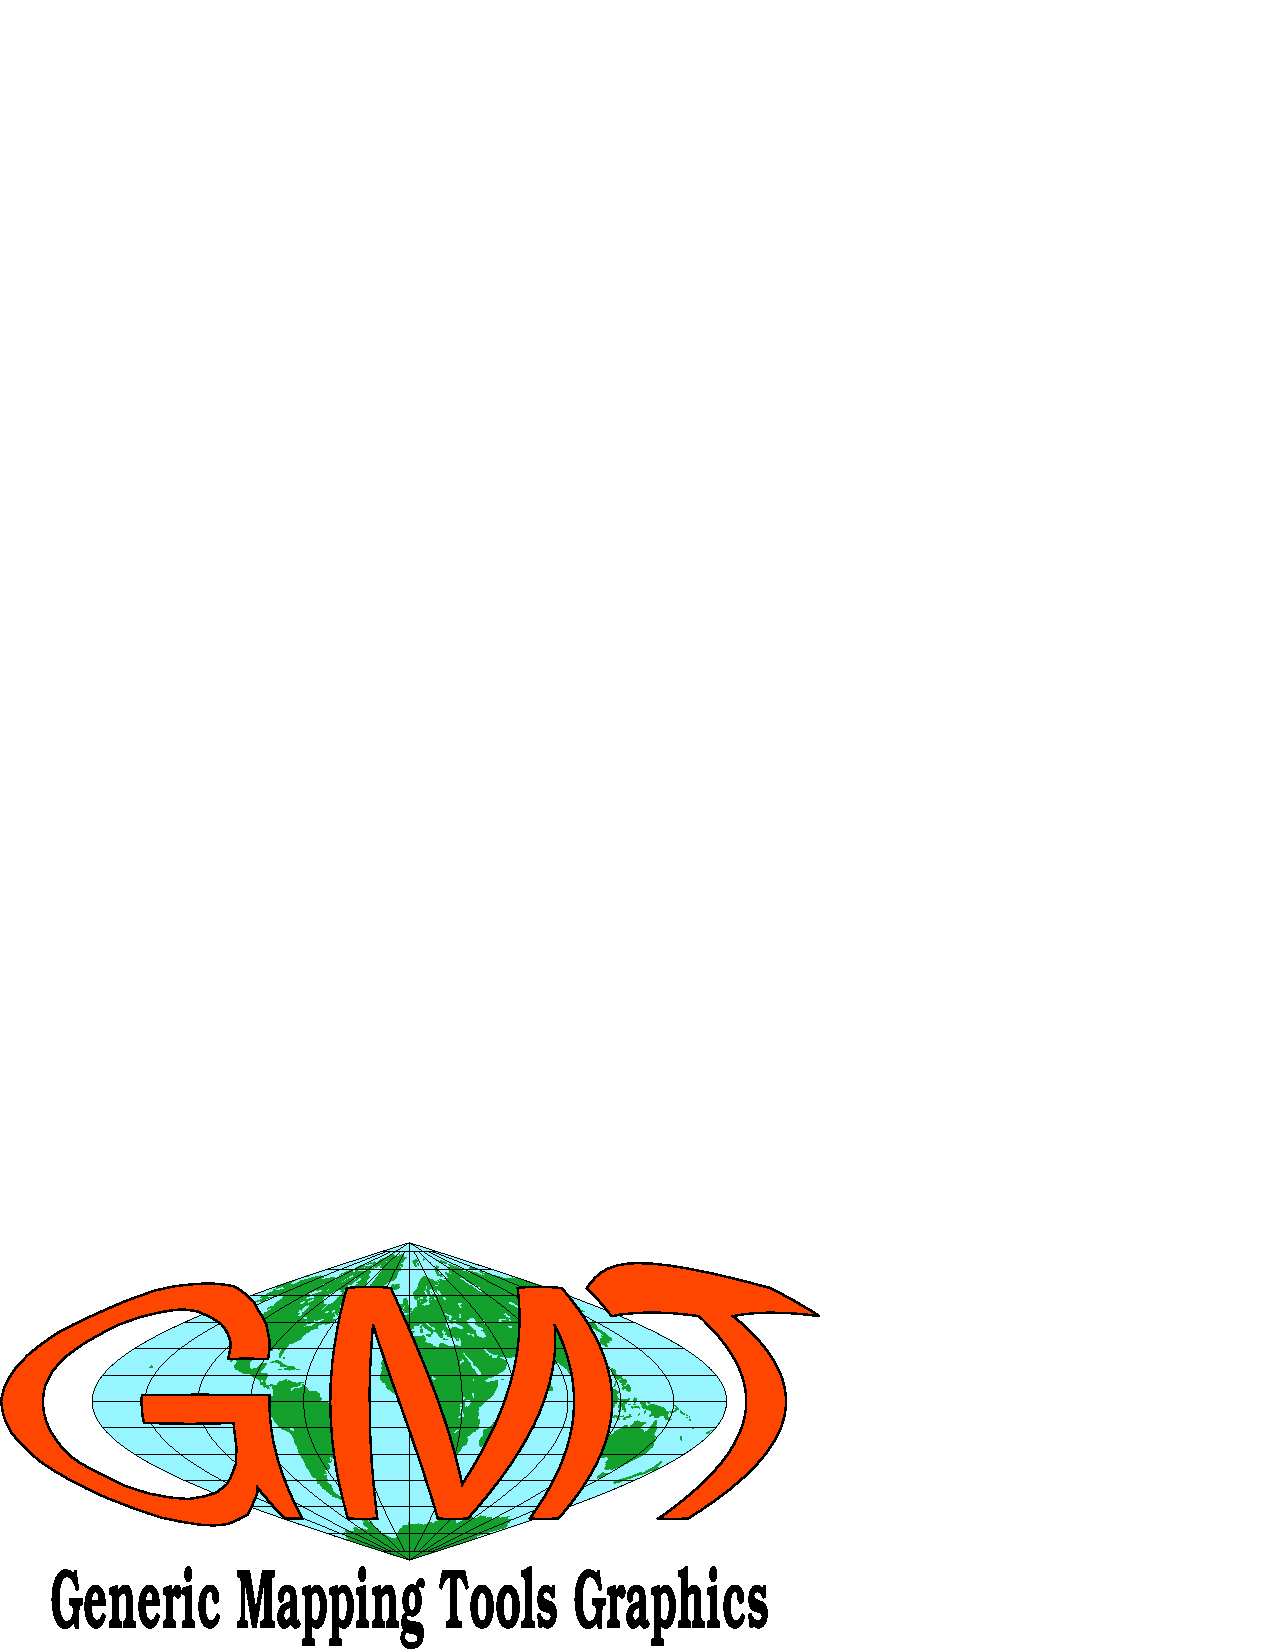
\includegraphics{GMT_coverlogo}
\end{center}

\clearpage

\pagestyle{plain}
\addcontentsline{toc}{chapter}{Contents}
\tableofcontents

\clearpage
\addcontentsline{toc}{chapter}{List of tables}
\listoftables

\clearpage
\addcontentsline{toc}{chapter}{List of figures}
\listoffigures

%------------------------------------------
%       $Id$
%
%       The GMT Documentation Project
%	Copyright (c) 2000-2013.
%	P. Wessel, W. H. F. Smith, R. Scharroo, J. Luis and F. Wobbe
%------------------------------------------
%

%----------------------ACKNOWLEDGMENTS--------------------------

\chapter*{Acknowledgments}\index{Acknowledgments}
\addcontentsline{toc}{chapter}{Acknowledgments}

The Generic Mapping Tools (\GMT) could not have been designed without
the generous support of several people.  We gratefully acknowledge
A. B. Watts and the late W. F. Haxby for supporting our efforts on the original
version 1.0 while we were their graduate students at Lamont-Doherty
Earth Observatory.  Doug Shearer and Roger Davis patiently answered
many questions over e-mail.  The subroutine \texttt{gauss}
was written and supplied by Bill Menke.
Further development of versions 2.0--2.1 at SOEST would not have
been possible without the support from the HIGP/SOEST
Post-Doctoral Fellowship program to Paul Wessel.  Walter H. F. Smith
gratefully acknowledges the generous support of the C. H. and I. M.
Green Foundation for Earth Sciences at the Institute of Geophysics
and Planetary Physics, Scripps Institution of Oceanography, University
of California at San Diego.
\GMT\ series 3.x, 4.x, and 5.x owe their existence to grants
EAR-93-02272, OCE-95-29431, OCE-00-82552, OCE-04-52126, and OCE-1029874
from the National Science Foundation, which we gratefully acknowledge.

We would also like to acknowledge feedback, suggestions and bug reports
from
Michael Barck,
Manfred Brands,
Allen Cogbill,
Stephan Eickschen,
Ben Horner-Johnson,
John Kuhn,
Angel Li,
Andrew Macrae,
Alex Madon,
Ken McLean,
Greg Neumann,
Ameet Raval,
Georg Schwarz,
Richard Signell,
Peter Schmidt,
Dirk Stoecker,
Eduardo Su\'{a}rez,
Mikhail Tchernychev,
Malte Thoma,
David Townsend,
Garry Vaughan,
William Weibel,
and many others, including their advice
on how to make \GMT\ portable to a wide range of platforms.
John Lillibridge and Stephan Eickschen provided the original examples 11 and 32, respectively;
Hanno von Lom helped resolve early problems with DLL libraries for Win32;
Lloyd Parkes enabled indexed color images in \PS;
Kurt Schwehr maintains the \textsf{Fink} packages;
Wayne Wilson implemented the full general perspective projection;
Florian Wobbe added support for regular expressions;
and William Yip helped translate \GMT\ to POSIX ANSI C and incorporate netCDF 3.
The SOEST RCF staff (Ross Ishida, Pat Townsend, and Sharon Stahl) provided valuable help
on Linux, web, and CGI script issues.

\begin{flushright}
Honolulu, HI, Silver Spring, MD, Cornish, NH, and Faro, Portugal, \GMTDOCDATE
\end{flushright}

\noindent
\begin{figure}[H]
	\centering
	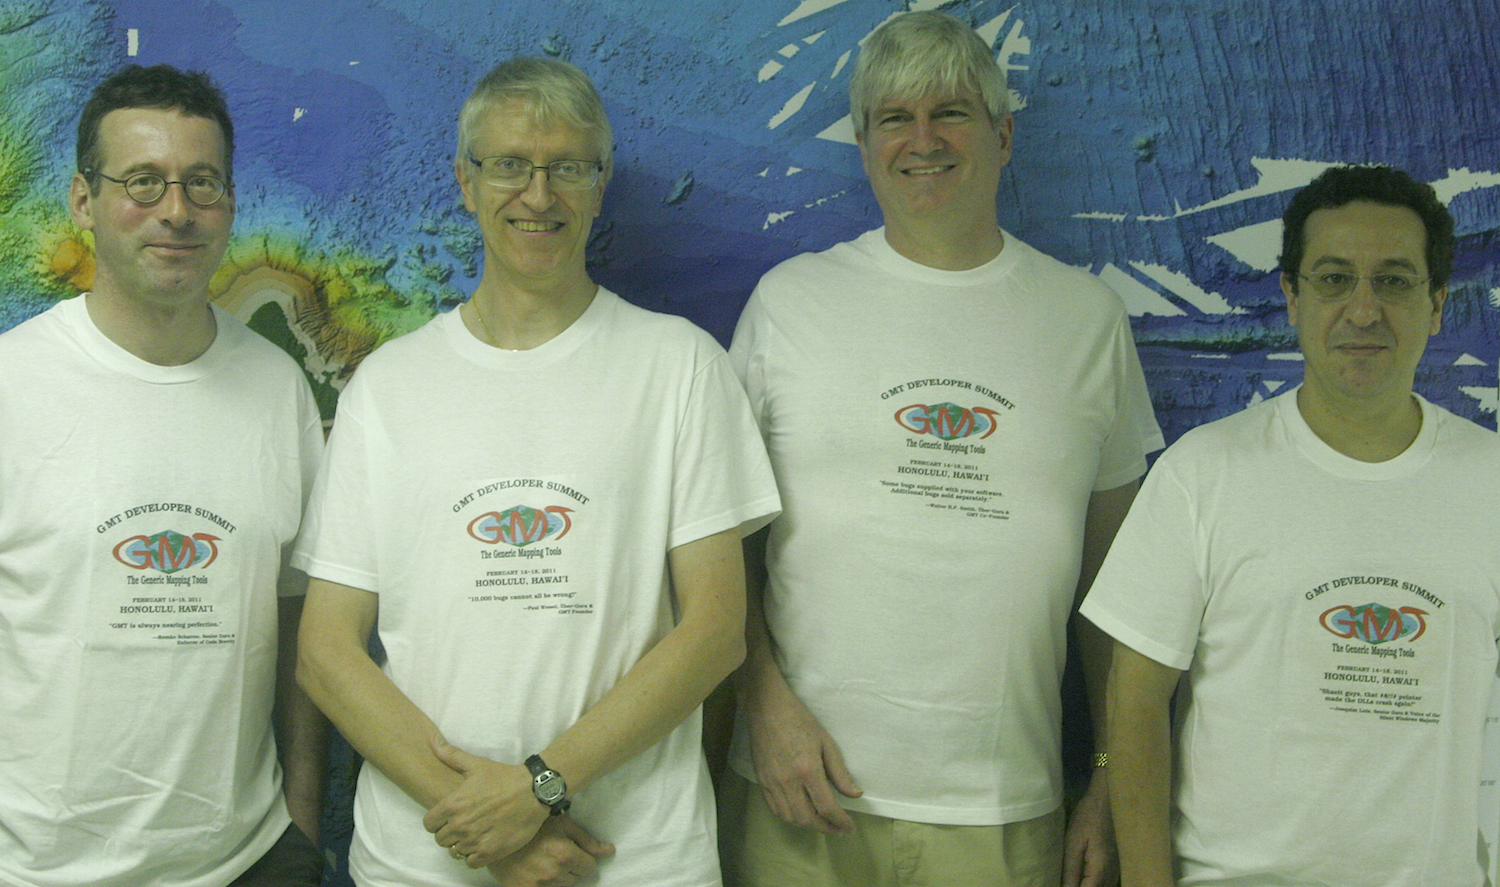
\includegraphics[width=\textwidth]{GMT5_Summit_2011.png}
	\caption{The four horsemen of the \GMT\ apocalypse: Remko Scharroo, Paul Wessel,
	Walter H.F. Smith, and Joaquim Luis at the \GMT\ Developer Summit in Honolulu,
	Hawaii during February 14--18, 2011.}
\end{figure}

%------------------------GMT DOCUMENTATION PROJECT---------------------------

\chapter*{The GMT Documentation Project}
\addcontentsline{toc}{chapter}{The GMT Documentation Project}

Starting with \GMT\ version 3.2, all \GMT\ documentation was
converted from Microsoft \progname{Word} to \LaTeX\ files.
This step was taken for a number of reasons:

\begin{enumerate}

\item Having all the documentation source available in
ASCII format makes it easier to access by several
\GMT\ developers working on different platforms in 
different countries.

\item \GMT\ scripts can now be included directly into the text
so that the documentation is automatically up-to-date
when scripts are modified.

\item All figures are generated on the fly and included as
\GMT\ EPS files which thus are always up-to-date.

\item It is easy to convert the \LaTeX\ files to other
formats, such as HTML, SGML, \PS, and PDF.

\item The whole task of assembling the pieces, be it generating
figures or extracting text portions from the master archive under
Subversion control, is automated by a makefile.

\item Only free software are used to maintain the \GMT\ Documentation.

\end{enumerate}

Please send email to
\htmladdnormallink{the GMT help list}{mailto:gmt-help@lists.hawaii.edu}
(subscription required; see Appendix D) if you find errors or inconsistencies in the documentation.
%--------------------------------REMINDER------------------------------------

\chapter*{A Reminder}
\addcontentsline{toc}{chapter}{A Reminder}

If you feel it is appropriate, you may consider paying us back by
citing our \emph{EOS} articles on \GMT\ (and perhaps also our Geophysics
article on the \GMT\ program \GMTprog{surface}) when you publish papers
containing results or illustrations obtained using \GMT.  The EOS
articles on \GMT\ are
\index{EOS article}%
\index{Article!in EOS}%

\begin{itemize}

\item{Wessel, P., and W. H. F. Smith, New, improved version of Generic
Mapping Tools released, \emph{EOS Trans. Amer. Geophys. U.}, vol. 79
(47), pp. 579, 1998.}

\item{Wessel, P., and W. H. F. Smith, New version of the Generic
Mapping Tools released, \emph{EOS Trans. Amer. Geophys. U.}, vol. 76
(33), pp. 329, 1995.}

\item{Wessel, P., and W. H. F. Smith, New version of the Generic
Mapping Tools released, \emph{EOS Trans. Amer. Geophys. U. electronic
supplement}, \htmladdnormallink{http://www.agu.org/eos\_elec/95154e.html}
{http://www.agu.org/eos\_elec/95154e.html}, 1995.}

\item{Wessel, P., and W. H. F. Smith, Free software helps map and
display data, \emph{EOS Trans. Amer. Geophys. U.}, vol. 72 (41),
pp. 441, 445-446, 1991.}

\end{itemize}
\noindent
Some \GMT\ programs are based on algorithms we have developed and
published, such as

\begin{itemize}

\item Kim, S.-S., and P. Wessel, Directional Median Filtering for Regional-Residual
Separation of Bathymetry, \emph{Geochem. Geophys. Geosyst., 9(Q03005)}, doi:10.1029/2007GC001850.
[\GMTprog{dimfilter.c} in \GMTprog{misc} supplement].

\item Smith, W. H. F., and P. Wessel, Gridding with Continuous
Curvature Splines in Tension, \emph{Geophysics}, vol. 55 (3), pp.
293--305, 1990 [\GMTprog{surface.c}].

\item Wessel, P., A General-purpose Green's Function-based Interpolator,
\emph{Computers \& Geosciences}, vol. 35, pp. 1247--1254, 2009  [\GMTprog{greenspline.c}].

\item  Wessel, P., Tools for Analyzing Intersecting Tracks: the x2sys package,
\emph{Computers \& Geosciences}, vol. 36, 348--354, 2010  [\GMTprog{x2sys} supplement].

\item Wessel, P. and J. M. Becker, Interpolation using a Generalized
Green's Function for a Spherical Surface Spline in Tension,
\emph{Geophys. J. Int.}, vol. 174, pp. 21--28, 2008  [\GMTprog{greenspline.c}].

\end{itemize}

\noindent
Finally, \GMT\ includes some code supplied by others, in particular the Triangle code
used for Delaunay triangulation.  Its author, Jonathan Shewchuk, says
\begin{quote}
``If you use Triangle, and especially if you use it to accomplish real
work, I would like very much to hear from you.  A short letter or email
(to jrs@cs.cmu.edu) describing how you use Triangle will mean a lot to
me.  The more people I know are using this program, the more easily I can
justify spending time on improvements and on the three-dimensional
successor to Triangle, which in turn will benefit you.''
\end{quote}

A few \GMT\ users take the time to write us letters, telling us of the
difference \GMT\ is making in their work.  We appreciate receiving these
letters.  On days when we wonder why we ever released \GMT\ we pull
these letters out and read them.  Seriously, as financial support for
\GMT\ depends on how well we can ``sell'' the idea to funding agencies and
our superiors, letter-writing is one area where \GMT\ users can affect
such decisions by supporting the \GMT\ project. 

%-------------------------COPYRIGHT----------------------------------

\chapter*{Copyright and Caveat Emptor!}
\index{Copyright}
\addcontentsline{toc}{chapter}{Copyright and Caveat Emptor!}

\begin{center}
Copyright \copyright 1991 -- \GMTDOCYEAR\ by P. Wessel, W. H. F. Smith, R. Scharroo, J. Luis and F. Wobbe
\end{center}

\vspace{\baselineskip}

The Generic Mapping Tools (\GMT) is free software; you can redistribute
it and/or modify it under the terms of the GNU Lesser General Public License
as published by the Free Software Foundation. \\

The \GMT\ package is distributed in the hope that it will be useful, but
WITHOUT ANY WARRANTY; without even the implied warranty of
MERCHANTABILITY or FITNESS FOR A PARTICULAR PURPOSE.  See the
file \filename{LICENSE.TXT} in the \GMT\ directory or the
\htmladdnormallinkfoot{GNU Lesser General Public License}{http://www.gnu.org/licenses/lgpl.html}
for more details. \\

Permission is granted to make and distribute verbatim copies of this
manual provided that the copyright notice and these paragraphs are
preserved on all copies.  The \GMT\ package may be included in a bundled
distribution of software for which a reasonable fee may be charged. \\

The Generic Mapping Tools (\GMT) does not come with any warranties,
nor is it guaranteed to work on your computer.  The user assumes full
responsibility for the use of this system. In particular, the School of
Ocean and Earth Science and Technology, the National Oceanic and
Atmospheric Administration, the National Science Foundation,
Paul Wessel, Walter H. F. Smith, or any other individuals involved in
the design and maintenance of \GMT\ are NOT responsible for any damage
that may follow from correct \emph{or} incorrect use of these programs.

%----------------------TYPOGRAPHIC CONVENTIONS------------------------

\chapter*{Typographic conventions}
\index{Typographic conventions}
\addcontentsline{toc}{chapter}{Typographic conventions}

In reading this documentation, the following provides a summary of
the typographic conventions used in this document.

\begin{enumerate}

\item User input and \GMT\ or \UNIX\ commands are indicated by
using the \texttt{typewriter} type style, e.g., \texttt{chmod +x job03.sh}.

\item The names of \GMT\ programs are indicated by the
\textsfbf{bold, sans serif} type style, e.g., we plot text with \textsfbf{pstext}.

\item The names of other programs are indicated by the
\textslbf{bold, slanted} type style, e.g., \textslbf{grep}.

\item File names are indicated by the \underline{underline}
type style, e.g., \underline{gmt.h}.

\end{enumerate}


\pagenumbering{arabic}
\pagestyle{headings}

%------------------------------------------
%	$Id: GMT_Chapter_1.tex,v 1.53 2006-10-29 01:38:25 pwessel Exp $
%
%	The GMT Documentation Project
%	Copyright 2000-2006.
%	Paul Wessel and Walter H. F. Smith
%------------------------------------------
%
\chapter{Preface} 
\label{ch:1}
\thispagestyle{headings}

While \GMT\ has served the map-making and data processing needs of scientists since 1988\footnote{Version
1.0 was then informally released at the Lamont-Doherty Earth Observatory.}, the current global use was
heralded by the first official release in {\it EOS Trans. AGU} in the fall of 1991.  Since then,
\GMT\ has grown to become a standard tool for many users, particularly in the Earth and Ocean Sciences.
Development has at times been rapid, and numerous releases have seen the light of day since the early
versions.  For a history of the changes from release to release, see the online
\htmladdnormallink{Release Announcements}{http://gmt.soest.hawaii.edu/gmt/gmt_releases.html}
and the file \filename{CHANGES} in the main \GMT\ directory.

The success of \GMT\ is to a large degree due to the input of the user community. In fact, most of the
capabilities and options in \GMT\ programs originated as user requests.
We would like to hear from you should you have any suggestions for future enhancements and modification.
Please send your comments to
\htmladdnormallink{the GMT help list}{mailto:gmt-help@hawaii.edu}.

\section{What is new in \gmt\ 4.x?}

\GMT\ 4.x continues to see both development of new features as well as corrections of
legacy bugs and problems.  It is likely we will continue to do so for a while until we
reach a stable point from which we can initiate the \GMT\ 5 development branch.  \GMT\ 5
will be distinguished by being completely restructured so as to allow developers to call
high-level \GMT\ processes from a variety of programming environments.  Below is a brief
history of the development milestones in the 4.x series.

\subsection{Overview of \gmt\ 4.1.4 [Nov-1, 2006]}

Changes in \GMT\ 4.1.4 are again relatively minor and predominantly bug fixes.  One imporant
new feature is that \GMT\ can now automatically recognize the format of the grd file given
to a program.  The use of the ``=id'' mechanism is now only needed when writing an output file in
a grid format other than the netCDF default.  We have also added
a new user directory pointed to by {\bf GMT\_USERDIR} (default directory is \filename{\~/.gmt})
where items such as \filename{.gmtdefaults4} will be looked for.  Additionally, a few enhancements
have been made to overcome limitations in the previous versions:

\begin{enumerate}
\item \GMTprog{grd2cpt} has a new option \Opt{T} for the creation of tables symmetric about zero.
\item \GMTprog{grdblend} will accept negative weights which are taken to mean that the sense of tapering should be reversed.
\item \GMTprog{grdedit} has a new option \Opt{E} to transpose the entire grid.
\item \GMTprog{grdreformat} now supports the \Opt{f} option.
\item \GMTprog{nearneighbor} will now optionally accept a {\it min\_sectors} argument appended to the \Opt{N} option.
\item \GMTprog{pshistogram}'s option \Opt{I} can now accept a modifier {\bf O} to output all bin data even if $y = 0$.
\item \GMTprog{psscale} will now invert the color scale if a negative length is provided, and if
\Opt{I} is given when \Opt{L}{\it gap} is in effect we will modify the constant colors accordingly.
\item \GMTprog{psxy} and \item \GMTprog{psxyz} have a new option \Opt{Sj}$|${\bf J} that plots a rotatable
rectangle but otherwise behaves similarly to \Opt{Se}$|${\bf E}.
\item \GMTprog{misc/ps2raster} has many improvements; added EPS output; high-quality PDF output.
Also removed -dDOINTERPOLATE option which caused inversion of colour map and had no benefits.
\end{enumerate}

Below is a list of previous problems (a few accidently introduced in \gmt\ 4.1.3)
that we have identified and corrected in the current release:

\begin{description}
\item [\GMTprog{gmt\_agc.c}]: AGC grids use 0 to represent NaNs -- this was not implemented yet.
\item [\GMTprog{gmt\_calclock.c}]: Proper rounding of time when converting to dates.
\item [\GMTprog{gmt\_support.c}]: Fixed bug in \Opt{I} when modifier {\bf =} was used.
\item [\GMTprog{gmt\_init.c}]: Fixed bug not recognizing {\bf PAGE\_ORIENTATION} as well as a bug that
prevented proper writing of {\bf PAGE\_ORIENTATION} in defaults.  Added a check so \GMTprog{gmtset}
will not crash if VALUE is not given.  Finally, let {\bf GMT\_HOMEDIR} default to C: under Windows
if {\bf HOME} is not set.
\item [\GMTprog{gmt\_grdio.c}]: Set [xy]\_units also in \GMTfunc{GMT\_update\_grd\_info}.
\item [\GMTprog{gmt\_nc.c}]: Made sure no garbage remains under Cygwin when using \GMTfunc{strncpy}.
\item [\GMTprog{gmt\_plot.c}]: Bugs related to annotations with \Opt{JPa} and its {\bf z} modifier fixed.
Log gridlines did not work for 3-D view.  3-D axis label would sometimes get misplaced due to round-off.
3-D map scale did not project correctly.  Duplicate title could appear if \Opt{JX} was used and one axis was geographic (d).
Needed to add secondary font to list to be encoded.
\item [\GMTprog{pslib.c}]: Fixed memory management in LZW compression (memory leak).  Improved EPS conformance.
\item [\GMTprog{filter1d}]: Robust option used extreme rather than median to determine the outliers.
\item [\GMTprog{gmtconvert}]: Did not have \Opt{L} listed in synopsis.
\item [\GMTprog{grdblend}]: Now skip grids that are entirely outside the region of interest.
\item [\GMTprog{grdcontour}]: Crashed if \Opt{M} and \Opt{D} were used with no file name specified.
\item [\GMTprog{grdcut}]: Require geographical instead of global in order to shift by 360 degrees.
\item [\GMTprog{grdfilter}]: Should not wrap over pole unless grid extends all the way to the pole.
\item [\GMTprog{grdinfo}]: When \Opt{C} was used there was no linefeed at the end.
\item [\GMTprog{grdsample}]: \Opt{T} did not ignore \Opt{R} (as per manual), resulting is changed cell size.
\Opt{F} did not use grid registration as default, rather that of input grid.
When using pixel registration, number of cells would be one too large.
\Opt{L} worked only in very limited case: going from x=[-180;180] to x=[0;360].
Now supports any periodicity in X and Y (as per manual). \Opt{F} again forces pixel registration.
Default is same as input.  More consistency with manual.
\item [\GMTprog{grdtrack}]: The \Opt{Z} option failed to be set for some input configurations.
\item [\GMTprog{grdvector}]: Added \Opt{f} option.
\item [\GMTprog{grdvolume}]: Three bugs squashed: gridcell oriented grids now get proper area and volume,
including edges; only one cell per NaN is excluded; when \Opt{C} and \Opt{L} are combined,
the volume is properly corrected for the baseline height.
\item [\GMTprog{pscoast}]: \Opt{N} and \Opt{I} reset pens to default settings after initially changing them.
Did not change output mode to binary (Windows only) if \Opt{M} and \Opt{b} were set.
\item [\GMTprog{pscontour}]: The \Opt{D} dump option wrote projected instead of original coordinates.
\item [\GMTprog{pslegend}]: Did not replace octagons with polygon form when pattern was requested.
Did not consider if absolute coordinates were given in \Opt{X} and \Opt{Y}. Passed the wrong character code
when {\bf M} was chosen with a plain scale modifier.
\item [\GMTprog{psscale}]: A vertical bar with a label placed along it was mis-justified.
\item [\GMTprog{pstext}]: Default for \Opt{G} is now {\bf BASEMAP\_FRAME\_RGB} as for other map annotations.
\item [\GMTprog{psxyz}]: \Opt{C} for symbols did not pick up color fill.
\item [\GMTprog{trend2d}]: Processing of \Opt{F} happened after checking.
\item [\GMTprog{xyz2grd}]: Had \Opt{Az} as default rather than no \Opt{A}.  Fixed bad header parsing when \Opt{E} was selected.
\item [\GMTprog{dbase/grdraster}]: Only do 360-degree wrapping if working on a geographic grid.
\item [\GMTprog{mgd77/mgd77list}]: Did not process time when \Opt{Am}2$|$4 was set and time was not requested as output.
Also, did not process time when \Opt{Am}2$|$4 was set and time was not requested as output.
\item [\GMTprog{x2sys/x2sys}]: Did not look in current dir for *.def files.
\end{description}

%-----------------------------------------
\subsection{Overview of \gmt\ 4.1.3 [June-1, 2006]}

Changes in \GMT\ 4.1.3 are relatively minor and predominantly bug fixes.  However, a few enhancements
have been made to overcome limitations in the previous versions:

\begin{enumerate}
\item Added the Hughes 1980 ellipsoid for projection support for DMSP SSM/I grid products.
\item \GMTprog{grdfft} has an extended \Opt{F} option to allow for either Gaussian- or
cosine-tapered filtering.
\item \GMTprog{psscale} now has a \Opt{Q} option so that logarithmic color scales and annotations
can be handled properly.
\item \GMTprog{makecpt} and \GMTprog{grd2cpt} have a new \Opt{M} option to allow the background, foreground, and
NaN-colors to be assigned using the \GMT\ defaults instead of the settings in the master CPT file. 
\item \GMTprog{mgd77list} in the {\bf mgd77} supplement has new option \Opt{Q} to specify limits on
speed and azimuths for output records.
\end{enumerate}

Below is a list of previous problems (some accidentily introduced in \gmt\ 4.1.2)
that we have identified and corrected in the current release:

\begin{description}
\item [\GMTprog{gmt\_grdio.c}]: Bug in \GMTfunc{GMT\_grd\_shift} for gridline-registered grids; this function is used in
\GMTprog{grdedit} to rotate grids of 360-degree longitudinal extent. Also added better testing for subsets of global (0-360) grids.
\item [\GMTprog{gmt\_init.c}]: \GMTfunc{GMT\_PS\_init} was called after --PAR=val had been decoded, resetting
the \PS-related parameters to their default settings.
\item [\GMTprog{gmt\_support.c}]: \GMTfunc{GMT\_set\_xy\_domain} padded region for pixel instead of grid registration,
which could cause SEGV in \GMTprog{xyz2grd} if ({\it x,y}) was less than half the grid-spacing outside region.
\item [\GMTprog{blockmean.c}]: The \Opt{C} option got reversed in 4.1.2 - now fixed.
\item [\GMTprog{blockmedian.c}]: The \Opt{C} option got reversed in 4.1.2 - now fixed.
\item [\GMTprog{grdcontour.c}]: The \Opt{C} option with a non-cpt file failed to read due to lack of proper if-test.
\item [\GMTprog{grdedit.c}]: The \Opt{S} option was backwards and tested {\it w-e}=360; should be {\it e-w}=360.
\item [\GMTprog{grdimage.c}]: Fixed bug introduced by \GMTfunc{GMT\_get\_inc} in 4.1.2. Internal projected
grid never took node\_offset from input grid.
\item [\GMTprog{grdmask.c}]: Polygons with zig-zag shape would sometimes cause a node exactly
on a polygon vertex to be considered inside. Radius was reset to 0 after \Opt{S}{\it radius} was assigned.
\item [\GMTprog{grdvector.c}]: The \Opt{A} option was not properly initiated.
\item [\GMTprog{psbasemap.c}]: The \Opt{L} option did not properly parse the optional :label:<just> part.
\item [\GMTprog{pslegend.c}]: If the {\bf M} (for map scale) was used, the \Opt{R} and \Opt{J} options would be reset.
Also prevented the undoing of \Opt{X} and \Opt{Y} at the end of the program.
\end{description}

%-----------------------------------------

\subsection{Overview of \gmt\ 4.1.2 [May-15, 2006]}

On the surface, changes in \GMT\ 4.1.2 are relatively minor.  Most of the work has involved
realignment of code and parsing of arguments to simplify the upcoming port to \GMT\ 5;
a brief listing of more visible changes include

\begin{enumerate}
\item Coastline files have been updated to use GSHHS version 1.4 which fixes minor inconsistencies
in the coastline database.
\item All coastline files are now stored in a new subdirectory \filename{coast} under the
\filename{share} directory, and the tar archives for coastlines now have their own version numbers
as they do not change as frequently as the source code.  Current coastline version number is 4.1.
\item The archives have been reorganized so that \filename{GMT\_share.*} contains all files needed
at runtime whereas the standard coastline files are in the new \filename{GMT\_coast.*} archive.
The \filename{GMT\_progs.*} archive has been renamed \filename{GMT\_src.*}.
\item CPT files can now have {\it z}-values that are date-time strings.
\item Optionally append {\bf z} to the \Opt{Jp} projection to annotate depths (i.e., ``north-y'') rather than radius.
\item Two new tools added to the {\bf misc} supplement for digitizing lines (\GMTprog{gmtdigitize.c}) and
to stitch digitized lines into continuous lines or polygons (\GMTprog{gmtstitch.c}).
\item Extended \Opt{M} option to take optional modifiers {\bf i} or {\bf o} for input or output.
\item Added support for custom grd format AGC from Atlantic Geoscience Center, assigned the code {\bf af} [21].
\end{enumerate}

A few programs or options have received minor updates and new features, such as

\begin{description}
\item [\GMTprog{blockmean.c}]: Added \Opt{E} for reporting standard deviation, min, and max values per block.
\item [\GMTprog{blockmedian.c}]: Added \Opt{E} for reporting L1 scale, min, and max values per block.
Also added \Opt{T} to specify a particular quartile [Default {\it q} = 0.5 = median].
\item [\GMTprog{blockmode.c}]: Added \Opt{E} for reporting LMS scale, min, and max values per block.
\item [\GMTprog{configure}]: Added explicit options to bypass the installation of supplements
that require Matlab (--disable-mex) and X11 (--disable-xgrid).
\item [\GMTprog{gmtconvert.c}]: Added \Opt{D} option to write segments to individual output files.
\item [\GMTprog{gmtdefaults.c}]: Support for new default {\bf PS\_VERBOSE} which controls the
writing of comments to \PS\ files.  {\bf COLOR\_MODEL} can now accept a prefix ``+'' which
forces color interpolation in the selected system (RGB or HSV only).  Default remains RGB.
{\bf PS\_COLOR} has been extended to accept HSV as well (only applies to
polygon, symbol, pen, and text colors, not images.).  New parameter {\bf POLAR\_CAP} which
controls the number of gridlines that converge on the poles for azimuthal and some other projections.
Added new default {\bf HISTORY} [TRUE] which controls whether or not we maintain a common command option
history via .gmtcommands4 files.
\item [\GMTprog{gmtmath.c}]: Added option \Opt{M} to indicate the program can now handle multisegment files.
Added {\bf CPOISS} for cumulative Poisson distribution.
\item [\GMTprog{grdmath.c}]: Added {\bf CPOISS} for cumulative Poisson distribution.
\item [\GMTprog{minmax.c}]: \Opt{D} made obsolete by improved range checking for longitudes (but available for
backwards compatibility).
\item [\GMTprog{psscale.c}]: Enhanced \Opt{I} option for asymmetrical intensity ranges from {\it low} to {\it high}.
\item [\GMTprog{psxy.c}]: Added \Opt{SW} for wedges defined by azimuths rather than directions.  Polygons of large
longitudinal extent now clip correctly.
\item [\GMTprog{splitxyz.c}]: New option \Opt{Q} to specify the output columns and their order.
\end{description}

Below is a list of previous problems
that we have identified and corrected in the current release:

\begin{description}
\item [\GMTprog{gmt\_plot.c}]: The 3-D perspective plotting of text was not scaled correctly.
\item [\GMTprog{gmt\_support.c}]: Parsing of \Opt{L} option used in \GMTprogi{psbasemap} and \GMTprogi{pscoast}
failed to get correct unit when ddd:mm:ss syntax was used for the position. Corner boundary conditions for grids (needed
by \GMTprog{grdtrack}, \GMTprog{grdsample}, \GMTprog{grdview}, and \GMTprog{grdgradient}) had the wrong sign.
\item [\GMTprog{gmt2rgb.c}]: Did not check name template properly, and did not initialize region.
\item [\GMTprog{gmtselect.c}]: Option \Opt{F} insisted on using spherical testing for Cartesian {\it x,y} data.
\item [\GMTprog{grd2xyz.c}]: The \Opt{E} option had the {\it y}-direction reversed.
\item [\GMTprog{grdfilter.c}]: Needed the \Opt{f} option to process \Opt{R}ddd:mm syntax.
\item [\GMTprog{grdimage.c}]: Would hang in {\it stdin} if \Opt{C} not given when one grid is plotted.
\item [\GMTprog{grdmask.c}]: Did not explicitly close polygons before using them.  Test for polar caps applied to the opposite pole.
\item [\GMTprog{grdmath.c}]: Command {\bf INSIDE} for Cartesian data had bug (passed {\it y} where {\it x} was expected).
\item [\GMTprog{grdsample.c}]: Failed when \Opt{I} was specified.
\item [\GMTprog{grdview.c}]: Bug in plotting north facade (\Opt{N}).  Also tried to free unallocated memory if \Opt{G} was used.
\item [\GMTprog{project.c}]: Cartesian projections gave incorrect results for {\it p,w,r,s}.
Removed 0--360 restriction on azimuth.  Option \Opt{G} was susceptible to round-off and thus
sometimes reissued the final point.
\item [\GMTprog{psxy.c}]: \Opt{SV} and \Opt{SE} for \Opt{JX} did not convert azimuths to directions.
The \Opt{Sq} option would get confused when distances between successive labels were smaller than the line's point spacing.
\item [\GMTprog{mgd77/mgd77manage.c}]: Did not properly close the file after ingesting E77 information.
\item [\GMTprog{pslib.c}]: \GMTfunc{ps\_load\_raster} did not use open mode {\bf rb} and hence failed under Windows.
\item [\GMTprog{xyz2grd.c}]: The \Opt{E} option had the {\it y}-direction reversed.
\item [\GMTprog{x2sys/x2sys\_get.c}]: \Opt{N} did not work properly (now fixed and tested).
\end{description}

%-----------------------------------------

\subsection{Overview of \gmt\ 4.1.1 [Mar-1, 2006]}

Changes in \GMT\ 4.1.1 are mostly minor; a brief listing include

\begin{enumerate}
\item \GMTprog{gmt\_nc.c}: Introduced handling of 4-D COARDS compliant grids (See Chapter 4 for details).
\item \GMTprog{mgd77/mngd77sniffer}: New tool for along-track quality control checking of MGD77 files.
\item \GMTprog{spotter/grdrotater}: New tool that rotates grids given a specified finite rotation.
\item Jonathan Shewchuk's triangulation routines are now stored with the rest of the source in the GMT\_progs.tar$|$zip archives.
(However, because his copyright is not GPL, installing it is still an option).
\end{enumerate}

A few programs or options have received minor updates and new features, such as

\begin{description}
\item [\GMTprog{grdedit}]: Added option \Opt{T} to toggle between gridline and pixel registrations (header only).
\item [\GMTprog{grdgradient}]: Implemented variation on Lambertian illumination.
\item [\GMTprog{grdmask}]: Now takes \Opt{S}{\it radius}[{\bf c$|$m$|$k$|$K}] as is done in \GMTprog{nearneighbor}.
\item [\GMTprog{gmtmath}]: If file is STDIN we read data from {\it stdin} and put the contents on the stack.
Also added \Opt{F} to select which columns to use for output [all].
\item [\GMTprog{grdtrack}]: Can now sample Sandwell/Smith IMG grids directly.
\item [\GMTprog{mgd77/mgd77.c}]: Added mechanism to search directories for files.
\item [\GMTprog{mgd77/mgd77list}]: Activated \Opt{X} option and associated machinery for applying data corrections.
\item [\GMTprog{psmask}]: -Now takes \Opt{S}{\it radius}[{\bf c$|$m$|$k$|$K}] as is done in \GMTprog{nearneighbor}.
Can now plot tiles regardless of projection and use patterns.
\item [\GMTprog{pstext}]: \Opt{D}[...]{\bf v}{\it pen} can now be used with or without \Opt{M}.
\item [\GMTprog{psxyz.c}]: \Opt{S}{\bf O}$|${\bf U} imitate \Opt{S}{\bf o}$|${\bf u} but without the 3-D color shading.
\end{description}

Inevitably, when new features are added, new bugs come along with them.  Below is a list of problems
that we have identified and corrected in the current release:.

\begin{description}
\item [\GMTprog{configure.in}]: Extracting VERSION from \GMTprog{gmt\_version.h}, not \GMTprog{gmt.h}.
\item [\GMTprog{gmt\_init.c}]: BASEMAP\_FRAME\_RGB overrode any changes to grid pens etc.  Now only
does so if prefixed by '+'.
\item [\GMTprog{gmt\_calclock.c}]: Did not allow \Opt{B}0 for time-axis.
\item [\GMTprog{gmt\_map.c}]: \Opt{JX}...{\bf d} now plots with WESN or degrees:minutes as per PLOT\_DEGREE\_FORMAT.
Map clip paths for \Opt{JE}{\it lon}/\PM 90 were no good.  Under certain circumstances, \GMTfunc{GMT\_non\_zero\_winding} might be passed
a polygon that was not closed, resulting in an error.  \Opt{JQ} would give garbage if central lon was way outside \Opt{R}.
\item [\GMTprog{gmt\_plot.c}]: \Opt{JX}...{\bf d} now plots with WESN or degrees:minutes as per PLOT\_DEGREE\_FORMAT.
\item [\GMTprog{gmt\_grdio.c}]: Changed logic to avoid false ``scale==0'' warning on Windows.
\GMTfunc{GMT\_open\_grd} (used in \GMTprog{grdblend}) reset scale to NaN.
Initialize header information at start of \GMTfunc{GMT\_read\_grd\_info}.
\item [\GMTprog{gmt\_support.c}]: Initialize [xyz]\_unit with more appropriate values.
Got wrong conversion for dx in meters to degrees.
\item [\GMTprog{gmt\_grd.h}]: Improved definition of \GMTfunc{GMT\_x\_to\_i} macro should reduce bugs
\item [\GMTprog{pslib.c}]: \GMTfunc{ps\_polygon}: if outline == -9 just fill and no clip.
Fixed two bugs concerning the /MaskColor operator.
\item [\GMTprog{ISO-8859-9.ps}]: Added /dotlessi per Onur Tan.
\item [\GMTprog{blockm*.c}]: Now correctly deals with periodic longitude data.
\item [\GMTprog{grdcontour.c}]: Fixed several issues at grid limits and inappropriate scaling of grid dimensions..
\item [\GMTprog{grdfilter.c}]: Used -1 as index flag instead of INT\_MIN.
\item [\GMTprog{grdimage.c}]: Fixed several issues at grid limits and inappropriate scaling of grid dimensions.
\item [\GMTprog{grdmask.c}]: Only let you change the value for outside nodes.
\item [\GMTprog{grdmath.man}]: Did not list \Opt{f} option.  Operators {\bf LT, LE, EQ, GE, GT} returned TRUE if NaNs were involved
Now NaN is returned if any of the two operands is a NaN.
\item [\GMTprog{grdreformat.c}]: Update grd.command before writing grid
\item [\GMTprog{grdvector.c}]: Did not place vectors correctly for pixel-pregistered grids.
\item [\GMTprog{grdview.c}]: Skipped nodes outside boundary but they might be needed to draw a tile.
\item [\GMTprog{pscoast.c}]: With \Opt{JE} and \Opt{G}{\it r/g/b}, the painting of the antipodal bin would incorrectly
turn off clipping, messing up the rest of the plot.  Now pass -9 to \GMTfunc{GMT\_fill} which means just fill and no end of clipping.
\item [\GMTprog{xyz2grd.c}]: For geographic grids with 360\DS\ range and gridline registration,
the west and east bin did not get replicated properly.
Now considers data inside the first and last tiles which might stick outside w/e/s/n.
\item [\GMTprog{x2sys/x2sys\_cross.c}]: Several problems fixed.
\end{description}

\subsection{Overview of \gmt\ 4.1 [Jan-7, 2006]}

Most changes in \GMT\ 4.1 are improvements ``under the hood''.  The most significant of these are

\begin{enumerate}
\item Addition of ability to both read and write netCDF files that are COARDS compliant.  This means
that \GMT, for the first time, is able to read netCDF files created by applications other than itself,
and that other applications capable of reading COARDS-compliant netCDF grids can directly import data
from \GMT.  We have added the new parameter {\bf GRID\_FORMAT} to the  \GMT\ defaults with ``nf'' as default.
Users who, against our recommendation, prefer to maintain the old non-COARDS compliant format as their
default grid format can instead select ``cf''. Support for extracting 2-D slices from 3-D netCDF grids has
also been added.
\item An overhaul of how the {\bf pslib} library encodes \PS\ images, resulting in vastly smaller files when
certain conditions are met, and general shrinking overall by enabling RLE or LZW compression.  We
have also added hooks for setting three new \PS\ parameters via \GMTprog{gmtdefaults} settings:
{\bf PS\_LINE\_CAP}, {\bf PS\_LINE\_JOIN}, and {\bf PS\_MITER\_LIMIT}. See \GMTprog{gmtdefaults} for details.
\item Improved alignment of strings ending in ``1'' in the \PS\ output.
\item Adjustments to how native \GMT\ grid headers are read and written in order to be fully 64-bit safe.
\GMT\ now runs in full 64-bit mode on platforms that supports it (e.g., Mac OS X G5).
\item Making \GMT\ tread-safe by replacing {\it strtok} with our own {\it GMT\_strtok} function.
\item Implemented full inverse Winkel map projection based on a new algorithm by Ipbuker, 2002,
{\it Cartography \& Geographical Information Science, 29}, 37-42.
\item Extended the options that is used to specify grid spacing (usually \Opt{I}{\it xinc/yinc}) to allow for
specifying {\it nx/ny} instead (by appending +).  Also, append ! to adjust the range so it fits exactly the
given increment [by default the range is kept fixed and sloppy increments are adjusted accordingly].
Append {\bf e}$|${\bf k}$|${\bf i}$|${\bf n} for increments in meter, km, miles
or nautical miles, respectively.  These increments are converted to degrees
longitude (at the middle latitude) and degrees latitude.
\item The polar $r, \theta$ projection \Opt{Jp} now takes an optional suffix {\bf r} that reverses the
radial coordinates (useful when $r$ is elevation as used by sky plots.)
\item The \GMTprog{misc} supplement has two new items: \GMTprog{ps2raster} uses \progname{ghostscript} to
fascilitate the rasterization of \PS\ files, while \GMTprog{nc2xy} allows extraction of data columns from
COARDS-compliant netCDF files.
\item The \GMTprog{mgd77} supplement has two new items: \GMTprog{mgd77convert} translates between different
MGD77 formats (including a new netCDF-based format), while \GMTprog{mgd77manage} assists in the management
of trackline data sets.
\item We now have improved PDF layout and navigation (thanks to Misha Tchernychev).
\item The HTML versions of all manual pages are now generated with \progname{groff}, and has active links
for \GMT\ Default parameters as they are references in the documentation.
\end{enumerate}

Many programs or options have received minor updates and new features, such as

\begin{description}
\item [\Opt{b}]: Ability to specify byte-swapping for native binary input and output tables by using upper
case {\bf S}$|${\bf D}.  This is useful if you have binary tables created on a little-endian machine (e.g.,
Linux PC) and need to read them on a big-endian machine (e.g., most RISC-chip machines from Sun, HP, Apple).
\item [\GMTprog{filter1d.c}]: Allow NaNs in all but the ``independent data'' column.
\item [\GMTprog{grdcontour.c}]: Label option {\bf +ap}[{\bf u}$|${\bf d}] for always having labels be readable up or down hills.
\item [\GMTprog{gmtconvert.c}]: New \Opt{N} option suppresses output records when all fields are NaNs.
\item [\GMTprog{gmtmath.c}]: Added {\bf TN} function
for evaluating Chebyshev polynomials; new constant {\bf Tn} was added to easily select normalized {\bf T}
(gives coordinates from -1 to + 1 suitable for evaluating Legendre and Chebyshev polynomials).
Finally, we added {\bf CORRCOEFF} for calculation of correlation coefficients, and \Opt{I} to reverse
the output by printing the last row first.
\item [\GMTprog{grd2cpt.c}]: New option \Opt{D} sets the back- and foreground colors to the colors at the limits of the cpt file.
\item [\GMTprog{grd2xyz.c}]: Added \Opt{E} for ESRI interchange ASCII grid dump.
\item [\GMTprog{grdfilter.c}]: Geographic boundary conditions are now in effect if \Opt{D4} is selected.
\item [\GMTprog{grdgradient.c}]: Added option \Opt{E} for Lambertian or Peuckeer illumination.
\item [\GMTprog{grdmath.c}]: Allow \Opt{bi} to be used with input files for commands {\bf PDIST}, {\bf LDIST},
and {\bf INSIDE}.  When spherical calculations are selected we now use the {\bf ELLIPSOID} setting to
determine if distance calculations should be along geodesics or great circles.  Also added {\bf TN} function
for evaluating Chebyshev polynomials; new constants {\bf Xn} and {\bf Yn} was added to easily select
normalized {\bf X} and {\bf Y}.  Finally, we added {\bf CORRCOEFF} for calculation of correlation coefficients.
\item [\GMTprog{grdraster.c}]: Optionally select a data set by giving a text pattern instead of data ID number.
This makes it easier to specify a certain data set (i.e., ``ETOPO2'') than having to remember its arbitrary numerical
ID.  Also, native grids with \GMT\ headers can also be placed in the database by appending {\bf H}{\it nbytes} to the
corresponding \filename{grdraster.info} entry, where {\it nbytes} is the size of the header that should be skipped
(use 892 for GMT headers).
\item [\GMTprog{makecpt.c}]: New option \Opt{D} sets the back- and foreground colors to the colors at the limits of the cpt file.
\item [\GMTprog{mapproject.c}]: \Opt{L} now outputs both the minimum distance and the coordinates
of the nearest point on the line.
\item [\GMTprog{pscoast.c}]: Added \Opt{Z} for 3-D map z-level (as in \GMTprog{psbasemap} and others).
\item [\GMTprog{pshistogram.c}]: New option \Opt{T}{\it col} lets user select any column to be used, starting
with 0 (first).  The old \Opt{2} option is retired (but remains accessible for backwards compatibility).  
\item [\GMTprog{psimage.c}]: Now support inclusion of EPS images.
\item [\GMTprog{pslegend.c}]: Added layout option {\bf B} for inserting color bars via \GMTprog{psscale}.
\item [\GMTprog{psscale.c}]: Now supports an optional {\bf ;}{\it label} at end of each line in cpt files.
If present this label will replace the default annotations when option \Opt{L} is used.
\item [\GMTprog{psxyz.c}]: Added \Opt{Q} to disable sorting of points based on distance.
\item [\GMTprog{sample1d.c}]: Allow NaNs in all but the ``independent data'' column.
\item [\GMTprog{xyz2grd.c}]: Added \Opt{E} for ESRI interchange ASCII grid digest.
\end{description}

Inevitably, when new features are added, new bugs come along with them.  Below is a list of problems
that we have identified and corrected in the current release:

\begin{description}
\item [\GMTprog{install\_gmt}]: No longer test netcdf installation since that can fail even when install was
successful [e.g., under Mac OS X Tiger].
\item [\GMTprog{gmt.h}]: \GMTfunc{GMT\_swab4} used {\tt unsigned long} instead of {\tt unsigned int} which could cause
64-bit problems.
\item [\GMTprog{gmt\_time\_system.h}]: Fixed MJD offsets by subtracting 10 days.
\item [\GMTprog{gmt\_calclock.c}]: time to hr,min,sec was vulnerable to round-off when optimized.  Also, {\it hh:mm} data
(without trailing {\it :ss}) would loose the minutes ({\it hh:mm:ss} was OK).
\item [\GMTprog{gmt\_grdio.c}]: Bug in scale/offset for \GMTprog{grdblend}'s row-by-row i/o.
\item [\GMTprog{gmt\_init.c}]: Would eat number with leading plus sign without checking if it actually was
a +\filename{gmtdefaults} file instruction; thus \GMTprog{gmtmath} could not see numbers such as +13.5.
Command line argument --{\bf BASEMAP\_FRAME\_RGB}={\it color} was not passed through to tick-, grid- and
annotation-properties.  \GMTfunc{GMT\_end} now frees memory used for hashing.  Did not use custom ellipsoid to set
DEG2M parameter so we got large errors for planets with significantly different radii.
\item [\GMTprog{gmt\_io.c}]: Bug in reading {\it yyyy}[/]{\it jjj} data fixed.  \GMTfunc{GMT\_lines\_init}
had trouble if 2000 segments had no data at all.  It also allocated 2000 points for each segment but never
deallocated the unused portions, thus running up memory fast.  \GMTfunc{GMT\_write\_segmentheader} wrote nothing
if input was binary and output is ASCII.  Fixed a few memory leaks.
\item [\GMTprog{gmt\_map.c}]: Azimuth to angle calculation for linear projections now properly handle different
scales in x and y. The calculation was also vulnerable to bad wrap-around, giving strange directions for
vectors in \GMTprog{psxy}. Geodesic distance calculation could get wrong quadrant.  
\item [\GMTprog{gmt\_plot.c}]: 360\DS\ polar basemaps could lack outline.  Direction for map roses were inaccurate.
Circle and $\theta$-$r$ boundaries did not allocate enough memory for arrays.  Would plot both -180 and +180 annotations
for periodic maps.
\item [\GMTprog{gmt\_shore.c}]: Must explicitly close polygons since inside/outside test in other programs expects it.
\item [\GMTprog{gmt\_support.c}]: Trouble extracting subregions of grid with {\it east} = 0.  Cartesian {\bf LDIST} failed
when mininum distance was requested (only done via \GMTprog{grdmath}).  Color names got truncated to 16 characters.
Improved workings of \GMTfunc{GMT\_sample\_cpt} in support of \GMTprog{makecpt}.  Fixed more memory leaks.
Bad LF/CR removal for \filename{coastline.conf} dir.
\item [\GMTprog{filter1d.c}]: \Opt{Ff} with even number of coefficients sometimes skip a coefficient.
\item [\GMTprog{gmtconvert.c}]: Missed first multisegment output header if input file was ASCII.
\item [\GMTprog{gmtmath.c}]: No longer have to say \Opt{Ca} if there is only one input column.  Did not understand
{\it date}{\bf T}{\it clock} as command line data.
\item [\GMTprog{gmtselect.c}]: If \Opt{M} is on and a portion of a segment is skipped, we must
reissue the multisegment header when segment resumes.  Now handles both Cartesian
and spherical polygons correctly.
\item [\GMTprog{grd2xyz.c}]: Sloppy \Opt{R} resulted in bad x,y values and sometimes allocation error.
\item [\GMTprog{grdfilter.c}]: Convolution filters now use correct area normalization.
\item [\GMTprog{grdgradient.c}]: If \Opt{M} is used with grids that include poles, ignore the poles
when normalizing the slopes.
\item [\GMTprog{grdimage.c}]: Cannot use \Opt{R} to extract subset when \Opt{J} is oblique.  Reverse log-axes did not work.
\item [\GMTprog{grdmask.c}]: Now handles both Cartesian and spherical correctly.
\item [\GMTprog{grdmath.c}]: Wrong sign in {\bf D2DY2}, and bogus value at {\it y = ymin}.  Now handles both Cartesian
and spherical polygons correctly.  Constants given on command line can now be absolute time, geographic coordinates, or
regular floating-point numbers.
\item [\GMTprog{grdtrack.c}]: Would fail to skip first two columns for ASCII input if dd:mm:ss format was used.
\item [\GMTprog{grdview.c}]: Cannot use \Opt{R} to extract subset when \Opt{J} is oblique.
\item [\GMTprog{grdvolume.c}]: \Opt{C}{\it low/high/delta} did not check for {\it low} < {\it high}, etc.
\item [\GMTprog{pscoast.c}]: Recursive painting could get tricked when boundaries were curved.
\item [\GMTprog{pslegend.c}]: Did not pass +\filename{gmtdefaults} and --{\bf PAR}={\it val} onto system calls.
\item [\GMTprog{psscale.c}]: Vertical annotations w/custom {\bf D\_FORMAT} were not aligned. Now uses more optimal means
to display the color bar, leading to smaller \PS\ files.  \Opt{E} did not flip sides when a negative width was used.
\item [\GMTprog{psxy.c}]: \Opt{Sp} is now a true point, but can also take an optional size.  Pentagon symbol had wrong
normalization scale.  If a fixed symbol size was given in \Opt{S}, with the symbol type supplied from file,
we would not scale symbols correctly if upper case symbols were given.
\item [\GMTprog{psxyz.c}]: Wrong index used in assigning color from cpt and in updating vector lengths.  If a fixed symbol
size was given in \Opt{S}, with the symbol type supplied from file,
we would not scale symbols correctly if upper case symbols were given
\item [\GMTprog{spectrum1d.c}]: Bugs in error expressions for admittance, gain, and phase have been corrected.
\item [\GMTprog{x2sys \& mgd77}]: Made DOS-format (CR/LF) tolerant.  Both supplements are now undergoing rapid
development.
\end{description}

\subsection{Overview of \gmt\ 4.0 [Oct-10, 2004]}

\GMT\ 4 represents a major overhaul of the package, hence the major version number increment.  There are four
categories of changes that have been implemented:
\begin{description}
\item [Time-series support.]  \GMT\ can now read and write time-series data where
the time coordinates are of the form {\it date}{\bf T}{\it clock}\footnote{Use standard
\UNIX\ tools such as \progname{awk} or \progname{perl} to reformat files should
your {\it date} and {\it clock} components reside in separate columns.}.  The formats
used for {\it date} and {\it clock} are under the user's control.  Both Gregorian
and ISO calendars are supported.  Frame annotation for time-series are now supported
via the \Opt{B} option; there are many new modifiers reflecting the vast number of
ways one may want to annotate time axes, including support for primary and secondary
annotation levels and the day- and month-names in numerous languages (send us the information
we need if your language is not supported).  The capability to handle time (in \Opt{R},
\Opt{J}, \Opt{B}, i/o, and plotting) required considerable changes ``under the hood'',
including the introduction of numerous new \GMTprog{gmtdefaults} parameters to make
the time series support as ``generic'' as we need it to be.
\item [New Tools.]  Three new tools have been added:
\begin{enumerate}
\item \GMTprog{gmt2rgb}: Makes red, green, and blue component gridfiles from an image (to be
used with new options for false color imaging or image draping by \GMTprog{grdimage} or \GMTprog{grdview}).
\item \GMTprog{grdblend}: Blends several partially over-lapping grdfiles into one combined grid.  Output
grid is written one row at the time so truly enormous grids can be created.
\item \GMTprog{pslegend}: Designs and plots elaborate legends on maps.
\end{enumerate}
\item [New Program Options.]  Many programs have received additional options or
features that enhances their usefulness:
\begin{itemize}
\item \GMTprog{blockmean}:	New option \Opt{Sw} will return weight sum while \Opt{Sz} returns
the data sums (i.e., it duplicates the previous \Opt{S} option).
\item \GMTprog{filter1d}:	New filters \Opt{Fl$|$L$|$u$|$U} that return extreme (min, max) values.
\item \GMTprog{gmtconvert}:	Added new options \Opt{F}, \Opt{A},  and \Opt{I} that simulate
\UNIX\ \progname{cut}, \progname{paste}, and \progname{tail} \Opt{r} (or \progname{tac}) capabilities.
Option \Opt{E} reports first and last point per segment only, \Opt{L} lists the segment headers only,
while \Opt{S} lists records from segments whose header matches a given text pattern.
\item \GMTprog{gmtmath}:	Added new operators for solving least squares problems ({\bf COL, LSQFIT}),
finding function roots ({\bf ROOTS}), and evaluating critical values ({\bf CHICRIT, FCRIT, TCRIT, ZCRIT}).
We also added some general functions ({\bf SINC, LOG2, LRAND}) and miscellaneous operations ({\bf FLIPUD, NEQ}).
The \Opt{S} option may now take a modifier to select first or last record only.
\item \GMTprog{gmtselect}:	New option  \Opt{Z} to pass or skip based on input $z$-range.
\item \GMTprog{grd2cpt}:	New options  \Opt{Q} for logarithmic scales, \Opt{E} for equidistant color
intervals, \Opt{R} for selecting a grid sub-region, and \Opt{N} to suppress output of B, F, N colors\footnote{Used
to color the background, foreground, and Not-a-Number areas.}.
\item \GMTprog{grd2xyz}:	New option \Opt{W} to write a constant weight factor as a 4th output column,
and ability to process several grid files at the same time.
\item \GMTprog{grdcontour}:	Expanded the \Opt{G} option to handle 5 algorithms (4 new) for the placement
of contour labels. 
\item \GMTprog{grdedit}:	New option \Opt{N} to replace selected node values given {\it x, y, z} data
in table form (options \Opt{H}, \Opt{b}, \Opt{f}, and \Opt{:} added for file support).
\item \GMTprog{grdfilter}:	New geospatial filters \Opt{Fl$|$L$|$u$|$U} that return extreme (min, max) values. 
\item \GMTprog{grdimage}:	New option for colormasking (\Opt{Q}; \PS\ Level 3 only), \PS\ image 
interpolation (\Opt{E}{\it -dpi}), and false RGB color image (when given three grids), as well as a modifier to \Opt{T}
to draw tile outlines.
\item \GMTprog{grdinfo}:	New option to create argument for \GMTprog{makecpt} (\Opt{T}) and to round-off
region boundary coordinates (\Opt{I}). 
\item \GMTprog{grdmath}:	Added new operators for critical values ({\bf CHICRIT, FCRIT, TCRIT, ZCRIT}),
geospatial analysis ({\bf LDIST,  PDIST, INSIDE}) and for calculating azimuths ({\bf CAS, SAZ}).  We have
also added some general functions ({\bf SINC, LOG2, LRAND}) and a few grid operations ({\bf FLIPLR, FLIPUD, ROTX, ROTY, NEQ,
INRANGE}).  We may now create multiple output grids from a single command.
\item \GMTprog{grdproject}: Option to supply false easting/northing or other offsets from the origin(\Opt{C}).
\item \GMTprog{grdreformat}: Option to suppress header in raw output (\Opt{N}).
\item \GMTprog{grdsample}:	Option to push the bilinear interpolation closer to nodes that are NaN (\Opt{Q}).
\item \GMTprog{grdtrack}:	Options to retrieve nearest node value (\Opt{N}, no interpolation) and to push
the bilinear interpolation closer to nodes that are NaN (\Opt{Q}).
\item \GMTprog{grdview}:	Colormasking (\Opt{Qc}, PS Level 3 only), draping of images via red, green,
and blue component grids (\Opt{G}).  Also,  drapegrids can have higher resolution than the relief grid, and we
added a modifier to \Opt{T} to draw tile outlines.
\item \GMTprog{makecpt}:	New options \Opt{Q} for logarithmic scales and \Opt{N} to suppress output
of B, F, N colors.
\item \GMTprog{mapproject}:	New options for datum conversions (\Opt{T}, \Opt{E}, and \Opt{Q}), azimuth and
back-azimuth (\Opt{A}), distance to point (\Opt{G}) and line  (\Opt{L})calculations, and optional false easting/northing (\Opt{C}).
\item \GMTprog{minmax}:		Added \Opt{T}{\it dz} option to produce \Opt{T} string for \GMTprog{makecpt},
\Opt{E} for returning extreme records, and the \Opt{I} option was extended to handle any number of columns when \Opt{C} is used.
\item \GMTprog{psbasemap}:	Extended \Opt{L} to allow alternate label and justification, and added \Opt{T}
for directional rose ornament or magnetic compass directions.
\item \GMTprog{pscoast}:	Extended \Opt{L} to allow alternate label and justification, and added \Opt{T}
for directional rose ornament or magnetic compass directions.
\item \GMTprog{pscontour}:	Expanded the \Opt{G} option to handle 5 algorithms (4 new) for the placement
of contour labels. 
\item \GMTprog{psimage}:	\PS\ image interpolation (\Opt{W}{\it -xlength}), and justification option
in \Opt{C}.
\item \GMTprog{psscale}:	Options to annotate on opposite side (\Opt{A}) and to plot back or foreground
triangle only (\Opt{E}[{\bf b$|$f}] ).  Also, draw discrete color-key table with centered annotations by appending an optional
{\it gap} to the \Opt{L} option. 
\item \GMTprog{pstext}: 	New option \Opt{A} should azimuths rather than angles be given,
\item \GMTprog{psxy}: 	Line color control (via \Opt{C}), symbol position offset (with \Opt{D}), custom symbols access 
(with \Opt{Sk}; use any of the 35 (Appendix~\ref{app:N}) that come with \GMT\ or design your own), many new symbols (horizontal and vertical dashes,
pentagon, octagon, rectangle, double-headed and centered vectors), and annotated (``quoted'') lines with \Opt{Sq}.
\item \GMTprog{psxyz}: 	Same, plus a vertical dash symbol.
\item \GMTprog{xyz2grd}: 	Added \Opt{Au$|$l} for upper/lower value at each node.
\end{itemize}
\item [General enhancements.]  These affect most of the programs:
\begin{itemize}
\item The coastline data have been updated to GSHHS version 1.3.  About 50 or so polygons had lingering
crossovers and some had duplicate points or failed to close; these have now been fixed. Major
errors in the Puget Sound coastline have also been corrected.
\item New shorthand to repeat the most recently used projection (\Opt{J}).
\item Options for phase-shifting the stride and supplying a prefix for frame annotations (\Opt{B}).
\item Override \GMT\ defaults directly on the command line with any number of {--}{--}\emph{PAR=value} options.
\item Now choose from 63 ellipsoids and 223 datums, or use your own values.
\item Numerous new \GMT\ defaults parameters, mostly in support of time-series functionality.
\item Shorthand for global regions (\Opt{Rg} for \Opt{R}0/360/-90/90 and \Opt{Rd} for \Opt{R}-180/180/-90/90).
\item Full support for either RGB, HSV, or CMYK in pen/fill command-line options or in cpt files.
\item Support for English color names (e.g., red, lightbrown).
\item Choice of unit when specifying pen thickness (cm, inch, point).
\item Easier pen specification mechanism, with predefined names for certain pen thicknesses.
\item Centering of plots on current page with \Opt{Xc}, \Opt{Yc}.
\item More control over input/output table formats (\Opt{f}, \Opt{:}[{\bf i$|$o}]).
\item Ability to read and write NOAA/NGDC GRD98 grid format.
\item Ability to add additional fonts.
\item Custom paper media size (useful for posters and large maps).
\item All text are now justified by the \PS\ interpreter, as is the clipping of contours and ``quoted lines''
to make space for annotation labels.
\item Better support for various international character encodings.
\item New Appendices M (color tables), N (custom symbols), O (contours and ``quoted lines''), and P
(using both \GMT\ 3 and 4).
\item New hidden files \filename{.gmtdefaults4} and \filename{.gmtcommands4} to ensure peaceful coexistence with \GMT\ 3-series.
\item Data files in directories pointed to by the three environmental parameters {\bf \$GMT\_DATADIR}, {\bf \$GMT\_GRIDDIR},
and {\bf \$GMT\_IMGDIR} can be specified without their full path names when used as input files.
\item We have added five new examples for a total of 25.
\item Bourne shell utility \progname{gmtswitch} simplifies switching between installed \GMT\ versions.
\end{itemize}
\end{description}


%------------------------------------------
%	$Id: GMT_Chapter_2.tex,v 1.21 2007-09-18 01:32:32 remko Exp $
%
%	The GMT Documentation Project
%	Copyright 2000-2007.
%	Paul Wessel and Walter H. F. Smith
%------------------------------------------
%
\chapter{Introduction}
\label{ch:2}
\thispagestyle{headings}

Most scientists are familiar with the sequence:
{\it raw data $\rightarrow$ processing $\rightarrow$ final illustration}.
In order to finalize papers for submission to scientific journals,
prepare proposals, and create overheads and slides for various
presentations, many scientists spend large amounts of time and
money to create camera-ready figures.  This process can be tedious
and is often done manually, since available commercial or in-house
software usually can do only part of the job.  To expedite this
process we introduce the Generic Mapping Tools (\GMT\ for short),
which is a free\footnote{See GNU General Public Licence
(www.gnu.org/copyleft/gpl.html) for terms on
redistribution and modifications.}, software package that can be used
to manipulate columns of tabular data, time-series, and gridded
data sets, and display these data in a variety of forms ranging
from simple {\it x}-{\it y} plots to maps and color, perspective,
and shaded-relief illustrations.  \GMT\ uses the \PS\
page description language [{\it Adobe Systems Inc.}, 1990]\index{PostScript@\PS}.  With \PS, multiple plot
files can easily be superimposed to create arbitrarily complex
images in gray tones or 24-bit true color.  Line drawings, bitmapped
images, and text can be easily combined in one illustration.
\PS\ plot files are device-independent: The same file
can be printed at 300 dots per inch (dpi) on an ordinary laserwriter
or at 2470 dpi on a phototypesetter when ultimate quality is needed.
\GMT\ software is written as a set of \UNIX\ tools\footnote{The
tools can also be installed on other platforms (see Appendix~\ref{app:L}).}
and is totally self-contained and fully documented.  The system is offered free
of charge and is distributed over the computer
network (Internet) [{\it Wessel and Smith, 1991; 1995a,b; 1998}].

The original version 1.0 of \GMT\ was released in the summer of 1988
when the authors were graduate students at Lamont-Doherty Earth
Observatory\index{Lamont-Doherty Earth Observatory}\index{L-DEO} of Columbia University.
During our tenure as graduate
students, L-DEO changed its computing environment to a distributed
network of \UNIX\ workstations, and we wrote \GMT\ to run in this
environment.  It became a success at L-DEO, and soon spread to
numerous other institutions in the US, Canada, Europe, and Japan.
The current version benefits from the many suggestions
contributed by users of the earlier versions, and now includes more
than 50 tools, 25 map projections, and many other new, more
flexible features.  \GMT\ provides scientists with a variety of
tools for data mani\-pulation and display, including routines to sample,
filter, compute spectral estimates, and determine trends in time
series, grid or triangulate arbitrarily spaced data, perform
mathematical operations (including filtering) on 2-D data sets
both in the space and frequency domain, sample surfaces along
arbitrary tracks or onto a new grid, calculate volumes, and find
trend surfaces.  The plotting programs will let the user make linear,
log$_{10}$, and {\it x$^a$}--{\it y$^b$} diagrams, polar and
rectangular histograms, maps with filled continents and coastlines
choosing from 25 common map projections, contour plots, mesh plots,
monochrome or color images, and artificially illuminated
shaded-relief and 3-D perspective illustrations. 

\index{ANSI C compliant}
\index{POSIX compliant}
\index{Y2K compliant}
\index{Compliance!POSIX}
\index{Compliance!ANSI C}
\index{Compliance!Y2K}
\GMT\ is written in the highly portable ANSI C \index{ANSI C} programming language
[{\it Kernighan and Ritchie}, 1988], is fully POSIX compliant\index{POSIX}
[{\it Lewine}, 1991], has no Year 2000 problems\index{Year 2000 compliant}, and may be used
with any hardware running some flavor of \UNIX, possibly with minor
modifications.  In writing \GMT, we have followed the modular
design philosophy of \UNIX: The {\it raw data $\rightarrow$  processing $\rightarrow$
final illustration} flow is broken down to a series of elementary
steps; each step is accomplished by a separate \GMT\ or \UNIX\ tool.
This modular approach brings several benefits: (1) only a few
programs are needed, (2) each program is small and easy to update
and maintain, (3) each step is independent of the previous step
and the data type and can therefore be used in a variety of
applications, and (4) the programs can be chained together in
shell scripts or with pipes, thereby creating a process tailored
to do a user-specific task.  The  decoupling of the data retrieval
step from the subsequent massage and plotting is particularly
important, since each institution will typically have its own
data base formats.  To use \GMT\ with custom data bases, one has
only to write a data extraction tool which will put out data in a
form readable by \GMT\ (discussed below).  After writing the extractor,
all other \GMT\ modules will work as they are. 

\GMT\ makes full use of the \PS\ page description language, and can produce color illustrations
if a color \PS\ device is available.  One does not
necessarily have to have access to a top-of-the-line color printer
to take advantage of the color capabilities offered by \GMT: Several
companies offer imaging services where the customer provides a
\PS\ plot file and gets color slides or hardcopies in return.
Furthermore, general-purpose \PS\ raster image processors
(RIPs) are now becoming available, letting the user create raster images
from \PS\ and plot these bitmaps on raster devices like computer
screens, dot-matrix printers, large format raster plotters, and film
writers\footnote{One public-domain RIP is \progname{ghostscript},
available from www.gnu.org.}.
Because the publication costs of color illustrations are high,
\GMT\ offers 90 common bit and hachure patterns, including many geologic
map symbol types, as well as complete graytone shading operations.
Additional bit and hachure patterns may also be designed by the user.
With these tools, it is possible to generate publication-ready
monochrome originals on a common laserwriter. 

\GMT\ is thoroughly documented and comes with a technical reference and
cookbook which explains the purpose of the package and its many features,
and provides numerous examples to help new users quickly become familiar
with the operation and philosophy of the system.  The cookbook contains
the shell scripts that were used for each example; \PS\
files of each illustration are also provided.  All programs have
individual manual pages which can be installed as part of the on-line
documentation under the \UNIX\ \progname{man} utility or as web pages.  In addition, the
programs offer friendly help messages which make them essentially
self-teaching -- if a user enters invalid or ambiguous command arguments,
the program will print a warning to the screen with a synopsis of the
valid arguments.  All the documentation is avaliable for web browsing
and may be installed at the user's site.

The processing and display routines within \GMT\ are completely general
and will handle any ({\it x,y}) or ({\it x,y,z}) data as input.
For many purposes the ({\it x,y}) coordinates will be (longitude,
latitude) but in most cases they could equally well be any other
variables (e.g., wavelength, power spectral density).  Since the \GMT\
plot tools will map these ({\it x,y}) coordinates to positions on a
plot or map using a variety of transformations (linear, log-log, and
several map projections), they can be used with any data that are
given by two or three coordinates.  In order to simplify and standardize
input and output, \GMT\ uses two file formats only.  Arbitrary sequences
of ({\it x,y}) or ({\it x,y,z}) data are read from multi-column ASCII
tables, i.e., each file consists of several records, in which each
coordinate is confined to a separate column\footnote{Programs now also
allow for fast, binary multicolumn file i/o.}.  This format is
straightforward and allows the user to perform almost any simple
(or complicated) reformatting or processing task using standard
\UNIX\ utilities such as \progname{cut}, \progname{paste}, \progname{grep},
\progname{sed} and \progname{awk}.
Two-dimensional data that have been sampled on an equidistant grid are
read and written by \GMT\ in a binary grid file using the functions
provided with the netCDF\index{netCDF} library (a free, public-domain software
library available separately from UCAR, the University Corporation
of Atmospheric Research [{\it Treinish and Gough}, 1987]).  This XDR\index{XDR}
(External Data Representation) based format is architecture independent,
which allows the user to transfer the binary data files from one
computer system to another\footnote{While the netCDF format is the default,
other formats are also possible, including user-defined formats.}.
\GMT\ contains programs that will read ASCII
({\it x,y,z}) files and produce gridded files.  One such program,
\GMTprog{surface}, includes new modifications to the gridding algorithm
developed by {\it Smith and Wessel} [1990] using continuous splines
in tension. 

Most of the programs will produce some form of output, which falls
into four categories.  Several of the programs may produce more than
one of these types of output:\par 

\begin{enumerate}

\item{1-D ASCII Tables --- For example, a ($x,y$) series may be filtered and
the filtered values output.  ASCII output is written to the standard output stream.} 

\item{2-D binary (netCDF or user-defined) grid files -- Programs that grid
ASCII ($x,y,z$) data or operate on existing grid files produce this type of output.} 

\item{\PS\ -- The plotting programs all use the \PS\
page description language to define plots.  These commands are stored as ASCII
text and can be edited should you want to customize the plot beyond the options
available in the programs themselves.} 

\item{Reports -- Several \GMT\ programs read input files and report statistics
and other information.  Nearly all programs have an optional ``verbose''
operation, which reports on the progress of computation.  All programs feature
usage messages, which prompt the user if incorrect commands have been given.
Such text is written to the standard error stream and can therefore be
separated from ASCII table output.} 

\end{enumerate} 

\GMT\ is available over the Internet at no charge.  To obtain a copy, read
the relevant information on the \GMT\ home page \GMTSITE,
or email
\htmladdnormallink{listserv@hawaii.edu}{mailto:listserv@hawaii.edu}
a note containing the single message \\ 
\index{GMT@\GMT!Mailinglists}
\index{Mailinglists}
\index{GMT@\GMT!on CD-ROM}
\index{GMT@\GMT!obtaining}
\index{GMT@\GMT!home page}

\textbf{information gmt-group} \\

The listserver will mail you back a shell-script that you may run to obtain
all necessary programs, libraries, and support data.  After you obtain the
\GMT\ archive, you will find that it contains information on how to install
\GMT\ on your hardware platform and how to obtain additional files that you
may need or want.  The archive also contains a license agreement and
registration file.  We also maintain two electronic mailing lists you may
subscribe to in order to stay informed about bug fixes and upgrades (See
Chapter~\ref{ch:7}).

For those without net-access that need to obtain \GMT: Geoware
\htmladdnormallink{(http://www.geoware-online.com)}{(http://www.geoware-online.com)}
makes and distributes CD-R and DVD-R media with the \GMT\ package, compatible supplements, and
several Gb of useful Earth and ocean science data sets.  For more information send e-mail to
\htmladdnormallink{geoware@geoware-online.com}{mailto:geoware@geoware-online.com}. 

\GMT\ has served a multitude of scientists very well, and their responses
have prompted us to develop these programs even further.  It is our
hope that the new version will satisfy these users and attract new
users as well.  We present this system to the community in order to
promote sharing of research software among investigators in the US
and abroad. 

\section*{References}

\begin{enumerate}
\item Kernighan, B. W., and D. M. Ritchie, {\it The C programming language},
2nd edition, p. 272, Prentice-Hall, Englewood Cliffs, New Jersey, 1988.

\item Adobe Systems Inc., {\it PostScript Language Reference Manual},
2nd edition, p. 764, Addison-Wesley, Reading, Massachusetts, 1990.

\item Lewine, D., POSIX programmer's guide, 1st edition, p. 607, O'Reilly
\& Associates, Sebastopol, California, 1991. 

\item Treinish, L. A., and M. L. Gough, A software package for the
data-independent management of multidimensional data,
{\it EOS trans. AGU, 68, }633--635, 1987.

\item Smith, W. H. F., and P. Wessel, Gridding with continuous curvature
splines in tension, {\it Geophysics, 55, }293--305, 1990. 

\item Wessel, P., and W. H. F. Smith, New, improved version of Generic
Mapping Tools released, {\it EOS trans. AGU}, 79, 579, 1998. 

\item Wessel, P., and W. H. F. Smith, New version of the Generic
Mapping Tools released, {\it EOS trans. AGU}, 76, 329, 1995a. 

\item Wessel, P., and W. H. F. Smith, New version of the Generic
Mapping Tools released, {\it EOS electronic supplement, }
http://www.agu.org/eos\_elec/95154e.html, 1995b. 

\item Wessel, P., and W. H. F. Smith, Free software helps map and
display data, {\it EOS trans. AGU}, 72, 441 \& 445--446, 1991. 

\end{enumerate}

%------------------------------------------
%	$Id: GMT_Chapter_3.tex,v 1.21 2004-07-14 01:59:53 pwessel Exp $
%
%	The GMT Documentation Project
%	Copyright 2000-2004.
%	Paul Wessel and Walter H. F. Smith
%------------------------------------------
%

\chapter{\gmt\ overview and quick reference}
\index{GMT@\GMT!overview|(}
\thispagestyle{headings}

\section{\gmt\ summary}
The following is a summary of all the programs supplied with \GMT\
and a very short description of their purpose.  For more details,
see the individual \UNIX\ manual pages or the online web documentation. 
For a listing sorted by program purpose, see Section~\ref{sec:purpose}.
\begin{tabbing}
nearneighborxxxxx \=					\kill
\GMTprog{blockmean}	\>	L$_2$ ({\it x},{\it y},{\it z}) table data filter/decimator \\ 
\GMTprog{blockmedian}	\>	L$_1$ ({\it x},{\it y},{\it z}) table data filter/decimator \\ 
\GMTprog{blockmode}	\>	Mode estimate ({\it x},{\it y},{\it z}) table data filter/decimator \\ 
\GMTprog{filter1d}	\>	Filter 1-D table data sets (time series) \\ 
\GMTprog{fitcircle}	\>	Finds the best-fitting great or small circle for a set of points \\ 
\GMTprog{gmt2rgb}	\>	Convert Sun raster or grd file to red, green, blue component grids \\ 
\GMTprog{gmtconvert}	\>	Convert data tables from one format to another \\ 
\GMTprog{gmtdefaults}	\>	List the current default settings \\ 
\GMTprog{gmtmath}	\>	Mathematical operations on table data \\ 
\GMTprog{gmtselect}	\>	Select subsets of table data based on multiple spatial criteria \\ 
\GMTprog{gmtset}	\>	Change selected parameters in current \filename{.gmtdefaults4} file \\ 
\GMTprog{grd2cpt}	\>	Generate a color palette table from a gridded file \\ 
\GMTprog{grd2xyz}	\>	Conversion from 2-D gridded file to table data \\ 
\GMTprog{grdblend}	\>	Blend several partially over-lapping grdfiles onto one grid \\ 
\GMTprog{grdclip}	\>	Limit the {\it z}-range in gridded data sets \\ 
\GMTprog{grdcontour}	\>	Contouring of 2-D gridded data sets \\ 
\GMTprog{grdcut}	\>	Cut a sub-region from a gridded file \\ 
\GMTprog{grdedit}	\>	Modify header information in a 2-D gridded file \\ 
\GMTprog{grdfft}	\>	Perform operations on gridded files in the frequency domain \\ 
\GMTprog{grdfilter}	\>	Filter 2-D gridded data sets in the space domain \\ 
\GMTprog{grdgradient}	\>	Compute directional gradient from gridded files \\ 
\GMTprog{grdhisteq}	\>	Histogram equalization for gridded files \\ 
\GMTprog{grdimage}	\>	Produce images from 2-D gridded data sets \\ 
\GMTprog{grdinfo}	\>	Get information about gridded files \\ 
\GMTprog{grdlandmask}	\>	Create masking gridded files from shoreline data base \\ 
\GMTprog{grdmask}	\>	Reset grid nodes in/outside a clip path to constants \\ 
\GMTprog{grdmath}	\>	Mathematical operations on gridded files \\ 
\GMTprog{grdpaste}	\>	Paste together gridded files along a common edge \\ 
\GMTprog{grdproject}	\>	Project gridded data sets onto a new coordinate system \\ 
\GMTprog{grdreformat}	\>	Converts gridded files into other grid formats \\ 
\GMTprog{grdsample}	\>	Resample a 2-D gridded data set onto a new grid \\ 
\GMTprog{grdtrack}	\>	Sampling of 2-D gridded data set along 1-D track \\ 
\GMTprog{grdtrend}	\>	Fits polynomial trends to gridded files \\ 
\GMTprog{grdvector}	\>	Plotting of 2-D gridded vector fields \\ 
\GMTprog{grdview}	\>	3-D perspective imaging of 2-D gridded data sets \\ 
\GMTprog{grdvolume}	\>	Calculate volumes under a surface within specified contour \\ 
\GMTprog{makecpt}	\>	Make color palette tables \\ 
\GMTprog{mapproject}	\>	Transformation of coordinate systems for table data \\ 
\GMTprog{minmax}	\>	Report extreme values in table data files \\ 
\GMTprog{nearneighbor}	\>	Nearest-neighbor gridding scheme \\ 
\GMTprog{project}	\>	Project table data onto lines or great circles \\ 
\GMTprog{psbasemap}	\>	Create a basemap plot \\ 
\GMTprog{psclip}	\>	Use polygon files to define clipping paths \\ 
\GMTprog{pscoast}	\>	Plot [and fill] coastlines, borders, and rivers on maps \\ 
\GMTprog{pscontour}	\>	Contour or image raw table data by triangulation \\ 
\GMTprog{pshistogram}	\>	Plot a histogram \\ 
\GMTprog{psimage}	\>	Plot Sun rasterfiles on a map \\ 
\GMTprog{pslegend}	\>	Plot a legend on a map \\ 
\GMTprog{psmask}	\>	Create overlay to mask out regions on maps \\ 
\GMTprog{psrose}	\>	Plot sector or rose diagrams \\ 
\GMTprog{psscale}	\>	Plot grayscale or colorscale on maps \\ 
\GMTprog{pstext}	\>	Plot textstrings on maps \\ 
\GMTprog{pswiggle}	\>	Draw table data time-series along track on maps \\ 
\GMTprog{psxy}		\>	Plot symbols, polygons, and lines on maps \\ 
\GMTprog{psxyz}		\>	Plot symbols, polygons, and lines in 3-D \\ 
\GMTprog{sample1d}	\>	Resampling of 1-D table data sets \\ 
\GMTprog{spectrum1d}	\>	Compute various spectral estimates from time-series \\ 
\GMTprog{splitxyz}	\>	Split {\it xyz} files into several segments \\ 
\GMTprog{surface}	\>	A continuous curvature gridding algorithm \\ 
\GMTprog{trend1d}	\>	Fits polynomial or Fourier trends to $y = f(x)$ series \\ 
\GMTprog{trend2d}	\>	Fits polynomial trends to $z = f(x,y)$ series \\ 
\GMTprog{triangulate}	\>	Perform optimal Delauney triangulation and gridding \\ 
\GMTprog{xyz2grd}	\>	Convert an equidistant table {\it xyz} file to a 2-D gridded file
\end{tabbing}
\index{GMT@\GMT!overview|)}

\section{\gmt\ quick reference}
\index{GMT@\GMT!quick reference|(}
\label{sec:purpose}
Instead of an alphabetical listing, this section contains a summary
sorted by program purpose.  Also included is a quick summary of the
standard command line options and a breakdown of the \Opt{J} option
for each of the 25 map projections available in \GMT. \\

\begin{center}

\begin{tabular}{|ll|} \hline
\multicolumn{2}{|c|}{FILTERING OF 1-D AND 2-D DATA} \\ \hline\hline
\GMTprog{blockmean}	&	L$_2$ estimate ($x, y, z$) data filters/decimators \\ \hline
\GMTprog{blockmedian}	&	L$_1$ estimate ($x, y, z$) data filters/decimators \\ \hline
\GMTprog{blockmode}	&	Mode estimate ($x, y, z$) data filters/decimators \\ \hline
\GMTprog{filter1d}	&	Filter 1-D data (time series) \\ \hline
\GMTprog{grdfilter}	&	Filter 2-D data in space domain \\ \hline\hline
\multicolumn{2}{|c|}{PLOTTING OF 1-D and 2-D DATA} \\ \hline\hline
\GMTprog{grdcontour}	&	Contouring of 2-D gridded data\\ \hline
\GMTprog{grdimage}	&	Produce images from 2-D gridded data \\ \hline
\GMTprog{grdvector}	&	Plot vector fields from 2-D gridded data \\ \hline
\GMTprog{grdview}	&	3-D perspective imaging of 2-D gridded data \\ \hline
\GMTprog{psbasemap}	&	Create a basemap frame \\ \hline
\GMTprog{psclip}	&	Use polygon files as clipping paths \\ \hline
\GMTprog{pscoast}	&	Plot coastlines, filled continents, rivers, and political borders \\ \hline
\GMTprog{pscontour}	&	Direct contouring or imaging of {\it xyz} data by triangulation \\ \hline
\GMTprog{pshistogram}	&	Plot a histogram \\ \hline
\GMTprog{psimage}	&	Plot Sun rasterfiles on a map \\ \hline
\GMTprog{pslegend}	&	Plot a legend on a map \\ \hline
\GMTprog{psmask}	&	Create overlay to mask specified regions of a map \\ \hline
\GMTprog{psrose}	&	Plot sector or rose diagrams \\ \hline
\GMTprog{psscale}	&	Plot grayscale or colorscale \\ \hline
\GMTprog{pstext}	&	Plot textstrings \\ \hline
\GMTprog{pswiggle}	&	Draw anomalies along track \\ \hline
\GMTprog{psxy}		&	Plot symbols, polygons, and lines in 2-D \\ \hline
\GMTprog{psxyz}		&	Plot symbols, polygons, and lines in 3-D \\ \hline
\end{tabular}

\begin{tabular}{|ll|} \hline
\multicolumn{2}{|c|}{GRIDDING OF (X,Y,Z) TABLE DATA} \\ \hline\hline
\GMTprog{nearneighbor}	&	Nearest-neighbor gridding scheme \\ \hline
\GMTprog{surface}	&	Continuous curvature gridding algorithm \\ \hline
\GMTprog{triangulate}	&	Perform optimal Delauney triangulation on {\it xyz} data \\ \hline\hline
\multicolumn{2}{|c|}{SAMPLING OF 1-D AND 2-D DATA} \\ \hline\hline
\GMTprog{grdsample}	&	Resample a 2-D gridded data onto new grid \\ \hline
\GMTprog{grdtrack}	&	Sampling of 2-D data along 1-D track \\ \hline
\GMTprog{sample1d}	&	Resampling of 1-D data \\ \hline\hline
\multicolumn{2}{|c|}{PROJECTION AND MAP-TRANSFORMATION} \\ \hline\hline
\GMTprog{grdproject}	&	Transform gridded data to a new coordinate system \\ \hline
\GMTprog{mapproject}	&	Transform table data to a new coordinate system \\ \hline
\GMTprog{project}	&	Project data onto lines or great circles \\ \hline\hline
\multicolumn{2}{|c|}{INFORMATION} \\ \hline\hline
\GMTprog{gmtdefaults}	&	List the current default settings \\ \hline
\GMTprog{gmtset}	&	Command-line editing of parameters in the \filename{.gmtdefaults4} file \\ \hline
\GMTprog{grdinfo}	&	Get information about the content of gridded files \\ \hline
\GMTprog{minmax}	&	Report extreme values in table data files \\ \hline\hline
\multicolumn{2}{|c|}{MISCELLANEOUS} \\ \hline\hline
\GMTprog{gmtmath}	&	Reverse Polish Notation (RPN) calculator for table data \\ \hline
\GMTprog{makecpt}	&	Create GMT color palette tables \\ \hline
\GMTprog{spectrum1d}	&	Compute spectral estimates from time-series \\ \hline
\GMTprog{triangulate}	&	Perform optimal Delauney triangulation on xyz data \\ \hline
\multicolumn{2}{|c|}{CONVERT OR EXTRACT SUBSETS OF DATA} \\ \hline\hline
\GMTprog{gmt2rgb}	&	Convert Sun raster or grd file to red, green, blue component grids \\ \hline 
\GMTprog{gmtconvert}	&	Convert table data from one format to another \\ \hline
\GMTprog{gmtselect}	&	Select table data subsets based on multiple spatial criteria \\ \hline
\GMTprog{grd2xyz}	&	Convert 2-D gridded data to table data \\ \hline
\GMTprog{grdcut}	&	Cut a sub-region from a gridded file \\ \hline
\GMTprog{grdblend}	&	Blend several partially over-lapping grdfiles onto one grid \\ \hline
\GMTprog{grdpaste}	&	Paste together gridded files along common edge \\ \hline
\GMTprog{grdreformat}	&	Convert from one grid format to another \\ \hline
\GMTprog{splitxyz}	&	Split ($x, y, z$) table data into several segments \\ \hline
\GMTprog{xyz2grd}	&	Convert table data to 2-D gridded file \\ \hline\hline
\multicolumn{2}{|c|}{DETERMINE TRENDS IN 1-D AND 2-D DATA} \\ \hline\hline
\GMTprog{fitcircle}	&	Finds best-fitting great or small circles \\ \hline
\GMTprog{grdtrend}	&	Fits polynomial trends to gridded files ($z = f(x, y)$) \\ \hline
\GMTprog{trend1d}	&	Fits polynomial or Fourier trends to $y = f(x)$ series \\ \hline
\GMTprog{trend2d}	&	Fits polynomial trends to $z = f(x, y)$ series \\ \hline\hline
\multicolumn{2}{|c|}{OTHER OPERATIONS ON 2-D GRIDS} \\ \hline\hline
\GMTprog{grd2cpt}	&	Make color palette table from gridded file \\ \hline
\GMTprog{grdclip}	&	Limit the $z$--range in gridded data sets \\ \hline
\GMTprog{grdedit}	&	Modify grid header information \\ \hline
\GMTprog{grdfft}	&	Operate on gridded files in frequency domain \\ \hline
\GMTprog{grdgradient}	&	Compute directional gradients from gridded files \\ \hline
\GMTprog{grdhisteq}	&	Histogram equalization for gridded files \\ \hline
\GMTprog{grdlandmask}	&	Creates mask gridded file from coastline database \\ \hline
\GMTprog{grdmask}	&	Set grid nodes in/outside a clip path to constants \\ \hline
\GMTprog{grdmath}	&	Reverse Polish Notation (RPN) calculator for gridded files \\ \hline
\GMTprog{grdvolume}	&	Calculate volume under a surface within a contour \\ \hline
\end{tabular}

\clearpage

\index{Standardized command line options|(}
\index{\Opt{B} (set anotations and ticks)|(}
\index{\Opt{H} (header records)|(}
\index{\Opt{J} (set map projection)|(}
\index{Projection!azimuthal!Lambert|(}
\index{Lambert azimuthal projection \Opt{Ja} \Opt{JA}|(}
\index{\Opt{Ja} \Opt{JA} (Lambert azimuthal)|(}
\index{Projection!conic!Albers \Opt{Jb} \Opt{JB}|(}
\index{Albers conic projection \Opt{Jb} \Opt{JB}|(}
\index{\Opt{Jb} \Opt{JB} (Albers)|(}
\index{Projection!conic!Equidistant \Opt{Jd} \Opt{JD}|(}
\index{Equidistant conic projection \Opt{Jd} \Opt{JD}|(}
\index{Projection!cylindrical!Cassini \Opt{Jc} \Opt{JC}|(}
\index{Cassini projection \Opt{Jc} \Opt{JC}|(}
\index{\Opt{Jc} \Opt{JC} (Cassini)|(}
\index{Projection!azimuthal!equidistant|(}
\index{Azimuthal equidistant projection \Opt{Je} \Opt{JE}|(}
\index{\Opt{Je} \Opt{JE} (Azimuthal equidistant)|(}
\index{Projection!azimuthal!gnomonic|(}
\index{Gnomonic projection \Opt{Jf} \Opt{JF}|(}
\index{\Opt{Jf} \Opt{JF} (Gnomonic)|(}
\index{Projection!azimuthal!orthographic|(}
\index{Orthographic projection \Opt{Jg} \Opt{JG}|(}
\index{\Opt{Jg} \Opt{JG} (Orthographic)|(}
\index{Hammer projection \Opt{Jh} \Opt{JH}|(}
\index{Projection!miscellaneous!Hammer|(}
\index{\Opt{Jh} \Opt{JH} (Hammer)|(}
\index{Sinusoidal projection \Opt{Ji} \Opt{JI}|(}
\index{Projection!miscellaneous!Sinusoidal (\Opt{Ji} \Opt{JI})|(}
\index{\Opt{Ji} \Opt{JI} (Sinusoidal)|(}
\index{Projection!cylindrical!Miller \Opt{Jj} \Opt{JJ}|(}
\index{Miller cylindrical projection \Opt{Jj} \Opt{JJ}|(}
\index{\Opt{Jj} \Opt{JJ} (Miller)|(}
\index{Eckert IV and VI projection \Opt{Jk} \Opt{JK}|(}
\index{Projection!miscellaneous!Eckert IV and VI (\Opt{Jk} \Opt{JK})|(}
\index{\Opt{Jk} \Opt{JK} (Eckert IV and VI)|(}
\index{Projection!conic!Lambert \Opt{Jl} \Opt{JL}|(}
\index{Lambert conic projection \Opt{Jl} \Opt{JL}|(}
\index{\Opt{Jl} \Opt{JL} (Lambert conic)|(}
\index{Projection!cylindrical!Mercator \Opt{Jm} \Opt{JM}|(}
\index{Mercator projection \Opt{Jm} \Opt{JM}|(}
\index{\Opt{Jm} \Opt{JM} (Mercator)|(}
\index{Robinson projection \Opt{Jn} \Opt{JN}|(}
\index{Projection!miscellaneous!Robinson|(}
\index{\Opt{Jn} \Opt{JN} (Robinson)|(}
\index{Projection!cylindrical!oblique Mercator \Opt{Jo} \Opt{JO}|(}
\index{Oblique Mercator projection \Opt{Jo} \Opt{JO}|(}
\index{\Opt{Jo} \Opt{JO} (Oblique Mercator)|(}
\index{Projection!polar ($\theta, r$)|(}
\index{Polar ($\theta, r$) projection|(}
\index{\Opt{Jp} \Opt{JP} (Polar ($\theta, r$) projections)|(}
\index{Projection!cylindrical!equidistant \Opt{Jq} \Opt{JQ}|(}
\index{Equidistant cylindrical projection \Opt{Jq} \Opt{JQ}|(}
\index{\Opt{Jq} \Opt{JQ} (Cylindrical equidistant)|(}
\index{Winkel Tripel projection \Opt{Jr} \Opt{JR}|(}
\index{Projection!miscellaneous!Winkel Tripel|(}
\index{\Opt{Jr} \Opt{JR} (Winkel Tripel)|(}
\index{Projection!azimuthal!stereographic|(}
\index{Stereographic projection \Opt{Js} \Opt{JS}|(}
\index{\Opt{Js} \Opt{JS} (Stereographic)|(}
\index{Projection!cylindrical!transverse Mercator \Opt{Jt} \Opt{JT}|(}
\index{Projection!cylindrical!UTM \Opt{Ju} \Opt{JU}|(}
\index{Transverse Mercator projection \Opt{Jt} \Opt{JT}|(}
\index{UTM projection \Opt{Ju} \Opt{JU}|(}
\index{\Opt{Jt} \Opt{JT} (Transverse Mercator)|(}
\index{\Opt{Ju} \Opt{JU} (UTM)|(}
\index{Van der Grinten projection \Opt{Jv} \Opt{JV}|(}
\index{Projection!miscellaneous!Van der Grinten|(}
\index{\Opt{Jv} \Opt{JV} (Van der Grinten)|(}
\index{Mollweide projection \Opt{Jw} \Opt{JW}|(}
\index{Projection!miscellaneous!Mollweide|(}
\index{\Opt{Jw} \Opt{JW} (Mollweide)|(}
\index{Projection!linear|(}
\index{Projection!linear!Cartesian|(}
\index{Cartesian linear projection|(}
\index{Linear projection|(}
\index{\Opt{Jx} \Opt{JX} (Non-map projections)|(}
\index{Projection!logarithmic|(}
\index{Logarithmic projection|(}
\index{Projection!power (exponential)|(}
\index{Power (exponential) projection|(}
\index{Projection!linear!geographic|(}
\index{Geographic Linear projection|(}
\index{Projection!cylindrical!general \Opt{Jy} \Opt{JY}|(}
\index{General cylindrical projection \Opt{Jy} \Opt{JY}|(}
\index{\Opt{Jy} \Opt{JY} (General cylindrical)|(}
\index{\Opt{K} (continue plot)|(}
\index{\Opt{O} (overlay plot)|(}
\index{\Opt{P} (portrait orientation)|(}
\index{\Opt{R} (set region)|(}
\index{\Opt{U} (plot timestamp)|(}
\index{\Opt{V} (verbose mode)|(}
\index{\Opt{X} (shift plot in $x$)|(}
\index{\Opt{Y} (shift plot in $y$)|(}
\index{\Opt{b} (binary i/o)|(}
\index{\Opt{c} (set \# of copies)|(}
\index{\Opt{f} (formatting of i/o)|(}
\index{\Opt{:} (input is $y,x$, not $x,y$)|(}

\begin{tabular}{|ll|} \hline
\multicolumn{2}{|c|}{STANDARDIZED COMMAND LINE OPTIONS} \\ \hline\hline
\multicolumn{2}{|l|}{\Opt{B}[{\bf p}$|${\bf s}]{\it xinfo}[{\it /yinfo}[{\it /zinfo}]][{\it WESNZwesnz+}][{\it :.title:}] Tickmarks. Each {\it info} is} \\
\multicolumn{2}{|l|}{\hspace{0.2in}[{\bf t}]{\it stride}[$\pm${\it phase}][{\bf u}][{\bf l}$|${\bf p}][:"label":][:="prefix":][:,"unit":], where {\bf l} and {\bf p} apply to $\log_{10}$ axes only, and} \\
\multicolumn{2}{|l|}{\hspace{0.2in}type {\bf t} = \{{\bf a, A, f, g, i, I}\}; unit {\bf u} = \{{\bf c, C, d, D, h, H, K, k, m, M, o, O, r, R, u, U, y, Y}\}} \\
\multicolumn{2}{|l|}{\hspace{0.2in}The leading {\bf p}$|${\bf s} selects primary [Default] or secondary axis items} \\ \hline
\Opt{H}[{bf i}][{\it n\_headers}]		&	ASCII [input] tables have header record[s] \\ \hline
\Opt{J}	(upper case for width, lower case for scale) &	Map projection (see below) \\ \hline
\hspace{0.2in}\Opt{JA}$lon_0/lat_0/width$	&	Lambert azimuthal equal area \\ \hline
\hspace{0.2in}\Opt{JB}$lon_0/lat_0/lat_1/lat_2/width$	&	Albers conic equal area \\ \hline
\hspace{0.2in}\Opt{JC}$lon_0/lat_0/width$	&	Cassini cylindrical \\ \hline
\hspace{0.2in}\Opt{JD}$lon_0/lat_0/lat_1/lat_2/width$	&	Equidistant conic \\ \hline
\hspace{0.2in}\Opt{JE}$lon_0/lat_0/width$	&	Azimuthal equidistant \\ \hline
\hspace{0.2in}\Opt{JF}$lon_0/lat_0/horizon/width$	&	Azimuthal Gnomonic \\ \hline
\hspace{0.2in}\Opt{JG}$lon_0/lat_0/width$	&	Azimuthal orthographic \\ \hline
\hspace{0.2in}\Opt{JH}$lon_0/width$	&	Hammer equal area \\ \hline
\hspace{0.2in}\Opt{JI}$lon_0/width$	&	Sinusoidal equal area \\ \hline
\hspace{0.2in}\Opt{JJ}$lon_0/width$	&	Miller cylindrical \\ \hline
\hspace{0.2in}\Opt{JKf}$lon_0/width$	&	Eckert IV equal area \\ \hline
\hspace{0.2in}\Opt{JKs}$lon_0/width$	&	Eckert VI equal area \\ \hline
\hspace{0.2in}\Opt{JL}$lon_0/lat_0/lat_1/lat_2/width$	&	Lambert conic conformal \\ \hline
\hspace{0.2in}\Opt{JM}$width$ or \Opt{JM}$lon_0/lat_0/width$	&	Mercator cylindrical \\ \hline
\hspace{0.2in}\Opt{JN}$lon_0/width$	&	Robinson \\ \hline
\hspace{0.2in}\Opt{JOa}$lon_0/lat_0/az/width$	&	Oblique Mercator, 1:	origin and azimuth \\ \hline
\hspace{0.2in}\Opt{JOb}$lon_0/lat_0/lon_1/lat_1/width$	&	Oblique Mercator, 2:	two points \\ \hline
\hspace{0.2in}\Opt{JOc}$lon_0/lat_0/lon_p/lat_p/width$	&	Oblique Mercator, 3:	origin and pole \\ \hline
\hspace{0.2in}\Opt{JP}[{\bf a}$width$[$/origin$]	&	Polar [azimuthal] ($\theta, r$) (or cylindrical) \\ \hline
\hspace{0.2in}\Opt{JQ}$lon_0/width$	&	Equidistant cylindrical (Plate Carr\'{e}e) \\ \hline
\hspace{0.2in}\Opt{JR}$lon_0/width$	&	Winkel Tripel \\ \hline
\hspace{0.2in}\Opt{JS}$lon_0/lat_0/width$	&	General stereographic \\ \hline
\hspace{0.2in}\Opt{JT}$lon_0/width$	&	Transverse Mercator \\ \hline
\hspace{0.2in}\Opt{JU}$zone/width$	&	Universal Transverse Mercator (UTM) \\ \hline
\hspace{0.2in}\Opt{JV}$lon_0/width$	&	Van der Grinten \\ \hline
\hspace{0.2in}\Opt{JW}$lon_0/width$	&	Mollweide \\ \hline
\hspace{0.2in}\Opt{JX}$width$[{\bf l}$|${\bf p}$exp|${\bf T}$|${\bf t}][/$height$[{\bf l}$|${\bf p}$exp|${\bf T}$|${\bf t}]][{\bf d}]	&	Linear, log$_{10}$, $x^a$--$y^b$, and time \\ \hline
\hspace{0.2in}\Opt{JY}$lon_0/lat_s/width$	&	General cylindrical equal area \\ \hline
\Opt{K}	&	Append more PS later \\ \hline
\Opt{O}	&	This is an overlay plot \\ \hline
\Opt{P}	&	Select Portrait orientation \\ \hline
\Opt{R}{\it west/east/south/north}[{\it /zmin/zmax}][{\bf r}] & Specify Region of interest \\ \hline
\Opt{U}[{\it /dx/dy}/][{\it label}]	&	Plot time-stamp on plot \\ \hline
\Opt{V}	&	Run in verbose mode \\ \hline
\Opt{X}[{\bf a}]{\it off}	&	Shift plot origin in $x$-direction \\ \hline
\Opt{Y}[{\bf a}]{\it off}	&	Shift plot origin in $y$-direction \\ \hline
\Opt{b}[{\bf i}$|${\bf o}][{\bf s}][{\it ncol}]	&	Select binary input or output \\ \hline
\Opt{c}{\it copies}	&	Set number of plot copies [1] \\ \hline
\Opt{f}[{\bf i}$|${\bf o}]{\it colinfo}	&	Set formatting of ASCII input or output \\ \hline
\Opt{:}	&	Expect {\it y}/{\it x} input rather than {\it x}/{\it y} \\ \hline
\end{tabular}

\index{Standardized command line options|)}
\index{\Opt{B} (set anotations and ticks)|)}
\index{\Opt{H} (header records)|)}
\index{\Opt{J} (set map projection)|)}
\index{Projection!azimuthal!Lambert|)}
\index{Lambert azimuthal projection \Opt{Ja} \Opt{JA}|)}
\index{\Opt{Ja} \Opt{JA} (Lambert azimuthal)|)}
\index{Projection!conic!Albers \Opt{Jb} \Opt{JB}|)}
\index{Albers conic projection \Opt{Jb} \Opt{JB}|)}
\index{\Opt{Jb} \Opt{JB} (Albers)|)}
\index{Projection!cylindrical!Cassini \Opt{Jc} \Opt{JC}|)}
\index{Cassini projection \Opt{Jc} \Opt{JC}|)}
\index{\Opt{Jc} \Opt{JC} (Cassini)|)}
\index{Projection!conic!Equidistant \Opt{Jd} \Opt{JD}|)}
\index{Equidistant conic projection \Opt{Jd} \Opt{JD}|)}
\index{Projection!azimuthal!equidistant|)}
\index{Azimuthal equidistant projection \Opt{Je} \Opt{JE}|)}
\index{\Opt{Je} \Opt{JE} (Azimuthal equidistant)|)}
\index{Projection!azimuthal!gnomonic|)}
\index{Gnomonic projection \Opt{Jf} \Opt{JF}|)}
\index{\Opt{Jf} \Opt{JF} (Gnomonic)|)}
\index{Projection!azimuthal!orthographic|)}
\index{Orthographic projection \Opt{Jg} \Opt{JG}|)}
\index{\Opt{Jg} \Opt{JG} (Orthographic)|)}
\index{Hammer projection \Opt{Jh} \Opt{JH}|)}
\index{Projection!miscellaneous!Hammer|)}
\index{\Opt{Jh} \Opt{JH} (Hammer)|)}
\index{Sinusoidal projection \Opt{Ji} \Opt{JI}|)}
\index{Projection!miscellaneous!Sinusoidal (\Opt{Ji} \Opt{JI})|)}
\index{\Opt{Ji} \Opt{JI} (Sinusoidal)|)}
\index{Projection!cylindrical!Miller \Opt{Jj} \Opt{JJ}|)}
\index{Miller cylindrical projection \Opt{Jj} \Opt{JJ}|)}
\index{\Opt{Jj} \Opt{JJ} (Miller)|)}
\index{Eckert IV and VI projection \Opt{Jk} \Opt{JK}|)}
\index{Projection!miscellaneous!Eckert IV and VI (\Opt{Jk} \Opt{JK})|)}
\index{\Opt{Jk} \Opt{JK} (Eckert IV and VI)|)}
\index{Projection!conic!Lambert \Opt{Jl} \Opt{JL}|)}
\index{Lambert conic projection \Opt{Jl} \Opt{JL}|)}
\index{\Opt{Jl} \Opt{JL} (Lambert conic)|)}
\index{Projection!cylindrical!Mercator \Opt{Jm} \Opt{JM}|)}
\index{Mercator projection \Opt{Jm} \Opt{JM}|)}
\index{\Opt{Jm} \Opt{JM} (Mercator)|)}
\index{Robinson projection \Opt{Jn} \Opt{JN}|)}
\index{Projection!miscellaneous!Robinson|)}
\index{\Opt{Jn} \Opt{JN} (Robinson)|)}
\index{Projection!cylindrical!oblique Mercator \Opt{Jo} \Opt{JO}|)}
\index{Oblique Mercator projection \Opt{Jo} \Opt{JO}|)}
\index{\Opt{Jo} \Opt{JO} (Oblique Mercator)|)}
\index{Projection!polar ($\theta, r$)|)}
\index{Polar ($\theta, r$) projection|)}
\index{\Opt{Jp} \Opt{JP} (Polar ($\theta, r$) projections)|)}
\index{Projection!cylindrical!equidistant \Opt{Jq} \Opt{JQ}|)}
\index{Equidistant cylindrical projection \Opt{Jq} \Opt{JQ}|)}
\index{\Opt{Jq} \Opt{JQ} (Cylindrical equidistant)|)}
\index{Winkel Tripel projection \Opt{Jr} \Opt{JR}|)}
\index{Projection!miscellaneous!Winkel Tripel|)}
\index{\Opt{Jr} \Opt{JR} (Winkel Tripel)|)}
\index{Projection!azimuthal!stereographic|)}
\index{Stereographic projection \Opt{Js} \Opt{JS}|)}
\index{\Opt{Js} \Opt{JS} (Stereographic)|)}
\index{Projection!cylindrical!transverse Mercator \Opt{Jt} \Opt{JT}|)}
\index{Projection!cylindrical!UTM \Opt{Ju} \Opt{JU}|)}
\index{Transverse Mercator projection \Opt{Jt} \Opt{JT}|)}
\index{UTM projection \Opt{Ju} \Opt{JU}|)}
\index{\Opt{Jt} \Opt{JT} (Transverse Mercator)|)}
\index{\Opt{Ju} \Opt{JU} (UTM)|)}
\index{Van der Grinten projection \Opt{Jv} \Opt{JV}|)}
\index{Projection!miscellaneous!Van der Grinten|)}
\index{\Opt{Jv} \Opt{JV} (Van der Grinten)|)}
\index{Mollweide projection \Opt{Jw} \Opt{JW}|)}
\index{Projection!miscellaneous!Mollweide|)}
\index{\Opt{Jw} \Opt{JW} (Mollweide)|)}
\index{Projection!linear|)}
\index{Projection!linear!Cartesian|)}
\index{Cartesian linear projection|)}
\index{Linear projection|)}
\index{\Opt{Jx} \Opt{JX} (Non-map projections)|)}
\index{Projection!logarithmic|)}
\index{Logarithmic projection|)}
\index{Projection!power (exponential)|)}
\index{Power (exponential) projection|)}
\index{Projection!linear!geographic|)}
\index{Geographic Linear projection|)}
\index{Projection!cylindrical!general \Opt{Jy} \Opt{JY}|)}
\index{General cylindrical projection \Opt{Jy} \Opt{JY}|)}
\index{\Opt{Jy} \Opt{JY} (General cylindrical)|)}
\index{\Opt{K} (continue plot)|)}
\index{\Opt{O} (overlay plot)|)}
\index{\Opt{P} (portrait orientation)|)}
\index{\Opt{R} (set region)|)}
\index{\Opt{U} (plot timestamp)|)}
\index{\Opt{V} (verbose mode)|)}
\index{\Opt{X} (shift plot in $x$)|)}
\index{\Opt{Y} (shift plot in $y$)|)}
\index{\Opt{b} (binary i/o)|)}
\index{\Opt{c} (set \# of copies)|)}
\index{\Opt{f} (formatting of i/o)|)}
\index{\Opt{:} (input is $y,x$, not $x,y$)|)}

\index{GMT@\GMT!quick reference|)}

\end{center}

%------------------------------------------
%	$Id: GMT_Chapter_4.tex,v 1.134 2011-04-06 23:51:12 guru Exp $
%
%	The GMT Documentation Project
%	Copyright (c) 2000-2011.
%	P. Wessel, W. H. F. Smith, R. Scharroo, and J. Luis
%------------------------------------------
%
\chapter{General features}
\label{ch:4}
\thispagestyle{headings}

This section explains features common to all the programs
in \GMT\ and summarizes the philosophy behind the system.  Some
of the features described here may make more sense once you reach
the cook-book section where we present actual examples of their use. 

\section{\gmt\ units}
\index{GMT@\GMT!units|(}
\index{Dimensions|(}
\index{Units|(}

While \GMT\ has default units for both actual Earth distances and
plot lengths (dimensions) of maps, it is recommended that you specifically indicate
the units of your arguments by appending the unit character, as discussed below.

\subsection{Distance units}

\GMT\ programs that accept actual Earth length scales like search radii or distances can
handle a variety of units.  The choices are listed in Table~\ref{tbl:distunits};
simply append the desired unit to the distance value you supply.  A value without
a unit suffix will be consider to be in meters.  For example, a distance of
30 nautical miles should be given as 30{\bf n}.
\begin{table}[H]
\centering
\index{Distance units}%
\index{Units, distance}%
\begin{tabular}{|l|l||l|l|} \hline
\multicolumn{1}{|c|}{\emph{Suffix}} & \multicolumn{1}{c|}{\emph{Distance unit}} & \multicolumn{1}{|c|}{\emph{Suffix}} & \multicolumn{1}{c|}{\emph{Distance unit}} \\ \hline
{\bf d}	&	Degrees of arc		& {\bf m}	&	Minutes of arc  \\ \hline
{\bf e}	&	Meters [Default]	& {\bf M}	&	Statute miles   \\ \hline
{\bf f}	&	Feet 			& {\bf n}	&	Nautical miles  \\ \hline
{\bf k}	&	Kilometers		& {\bf s}	&	Seconds of arc  \\ \hline
\end{tabular}
\caption{Distance units recognized by \gmt\ command line switches.}
\label{tbl:distunits}
\end{table} 
The calculation of distances on Earth (or other planetary bodies) depends on the
ellipsoidal parameters of the body and the method of computation.  \GMT\ offers
three alternatives:

\subsubsection{Flat Earth distances}
Quick, but approximate ``Flat Earth'' calculations make a first-order correction
for the spherical nature of a planetary body by computing the distance between
two points A and B as
\begin{equation}
	d_f = R \sqrt{(\theta_A - \theta_B)^2 + \frac{\theta_A + \theta_B}{2}(\lambda_A - \lambda_B)^2},
	\label{eq:flatearth}
\end{equation}
where $R$ is the mean (or spherical) radius of the planet, $\theta$ is latitude, and the difference in longitudes, $\Delta \lambda$,
is adjusted for any jumps that might occur across Greenwich or the Dateline.  This approach is suitable
when the points you use to compute $d_f$ do not greatly differ in latitude and computation
speed is paramount. You can specify this mode of computation by using the {\bf -} prefix to
the specified distance (or to the unit itself in cases where no distance is required).
A search radius of 50 statute miles using this mode of computation might be \Opt{S-}50{\bf M}.

\subsubsection{Great circle distances}
This is the default distance calculation, which will also approximate the planetary body by a sphere of mean
radius $R$. However, we compute an exact distance between two points A and B on such a sphere via
the Haversine equation
\begin{equation}
	d_g = 2R \sin^{-1}  {\sqrt{\sin^2\frac{\theta_A - \theta_B}{2} + \cos \theta_A \cos \theta_B \sin^2 \frac{\lambda_A - \lambda_B}{2}} },
	\label{eq:greatcircle}
\end{equation}
This approach is suitable for most situations unless exact calculations for an ellipsoid
is required.  For instance, a search radius of 5000 feet using this mode of computation would be \Opt{S}5000{\bf f}.


\subsubsection{Geodesic distances}
For the most accurate calculations we use a full ellipsoidal formulation.  Currently,
we are using Rudoe's formula.  You select this mode of computation by using the {\bf +} prefix to
the specified distance (or to the unit itself in cases where no distance is required).
For instance, a search radius of 20 km using this mode of computation would be \Opt{S+}20{\bf k}.

\subsection{Length units}

\GMT\ programs can accept dimensional quantities and plot lengths
in \textbf{c}m, \textbf{i}nch,
or \textbf{p}oint (1/72 of an inch)\footnote{\PS\ definition.
In the typesetting industry a slightly different definition of point
(1/72.27 inch) is used.}.  There are two ways to ensure that \GMT\ understands
which unit you intend to use:

\begin{enumerate}
\item Append the desired unit to the dimension you supply.  This
way is explicit and clearly communicates what you intend, e.g.,
\Opt{X}4\textbf{c} means the length being passed to the \Opt{X} switch is 4 cm.

\item Set the parameter \textbf{PROJ\_LENGTH\_UNIT} to the desired unit.  Then, all
dimensions without explicit unit will be interpreted accordingly.

\end{enumerate}
The latter method is less secure as other users may have a different unit
set and your script may not work as intended.  We therefore recommend
you always supply the desired unit explicitly.
\index{GMT@\GMT!units|)}
\index{Dimensions|)}
\index{Units|)}

\section{\gmt\ defaults}
\label{sec:gmt.conf}
\subsection{Overview and the \protect\filename{gmt.conf}\ file}

\index{GMT@\GMT!defaults|(}
\index{Default settings|(}

\GMTfig[h]{GMT_Defaults_1a}{Some \gmt\ parameters that affect plot appearance.}

There are about 100 parameters which can be adjusted individually
to modify the appearance of plots or affect the manipulation of data.
When a program is run, it initializes all parameters to the \GMT\
defaults\footnote{Choose between SI and US default units by modifying
\filename{gmt.conf} in the \GMT\ share directory.},
then tries to open the file \filename{gmt.conf}
in the current directory\footnote{To remain backwards compatible with \GMT\ 3.4.x
we will also look for \filename{gmt.conf} but only if \filename{gmt.conf}
cannot be found.}.  If not found, it will look for that file in a sub-directory \filename{\~/.gmt} of your home directory, and finally in your home directory itself.  If successful, the program will read the
contents and set the default values to those provided in the file.
By editing this file you can affect features such as pen thicknesses
used for maps, fonts and font sizes used for annotations and labels,
color of the pens, dots-per-inch resolution of the hardcopy device,
what type of spline interpolant to use, and many other choices
(A complete list of all the parameters and their default values can
be found in the \GMTprog{gmt.conf} manual pages).  Figures
\ref{fig:GMT_Defaults_1a}, \ref{fig:GMT_Defaults_1b},
and \ref{fig:GMT_Defaults_1c} show the parameters that affect plots). You may create
your own \filename{gmt.conf} files by running \GMTprog{gmtdefaults}
and then modify those parameters you want to change.  If you want
to use the parameter settings in another file you can do so by
specifying \texttt{+<defaultfile>} on the command line.
This makes it easy to maintain several distinct parameter settings,
corresponding perhaps to the unique styles required by different
journals or simply reflecting font changes necessary to make
readable overheads and slides.  Note that any arguments given on
the command line (see below) will take precedent over the default
values.  E.g., if your \filename{gmt.conf} file has \emph{x}
offset = 1\textbf{i} as default, the \Opt{X}1.5\textbf{i} option will override the
default and set the offset to 1.5 inches. 

There are at least two good reasons why the \GMT\ default options
are placed in a separate parameter file:

\begin{enumerate}

\item It would not be practical to allow for command-line syntax
covering so many options, many of which are rarely or never
changed (such as the ellipsoid used for map projections).

\item It is convenient to keep separate \filename{gmt.conf}
files for specific projects, so that one may achieve a special
effect simply by running \GMT\ commands in the directory whose
\filename{gmt.conf} file has the desired settings.  For example,
when making final illustrations for a journal article one must often
standardize on font sizes and font types, etc.  Keeping all those
settings in a separate \filename{gmt.conf} file simplifies this
process and will allow you to generate those illustrations with the same settings later on.  Likewise, \GMT\ scripts that make figures for PowerPoint
presentations often use a different color scheme and font size than
output intended for laser printers.  Organizing these various scenarios
into separate \filename{gmt.conf} files will minimize headaches
associated with micro-editing of illustrations.

\GMTfig[h]{GMT_Defaults_1b}{More \gmt\ parameters that affect plot appearance.}

\end{enumerate}

\subsection{Changing \gmt\ defaults}

As mentioned, \GMT\ programs will attempt to open a file named
\filename{gmt.conf}.  At times it may be desirable to override
that default.  There are several ways in which this can be accomplished.
\begin{enumerate}
\item Supply another filename using the \emph{+filename} syntax, i.e.,
on the same command line as the \GMT\ command we append the name of
the alternate \filename{gmt.conf} file with the plus sign as a prefix.
Because any changes only apply to that one command you would have to
append the alternate file to every command in your script.  This is
tedious but may be an option for situations when you cannot write in
the current directory (e.g., some CGI scripts).
\item A perhaps less tedious method is to start each script by making a
copy of the current \filename{gmt.conf}, then copy the desired
\filename{gmt.conf} file to the current directory, and finally
undo the changes at the end of the script.  Possible side effects
include premature ending of the script due to user error or bugs which
means the final resetting does not take place (unless you write your
script very carefully.)
\item To permanently change some of the \GMT\ parameters on the fly
inside a script the \GMTprog{gmtset} utility can be used.  E.g., to
change the primary annotation font to 12 point Times-Bold we run \\

\texttt{gmtset FONT\_ANNOT\_PRIMARY 12p,Times-Bold} \\

These changes will remain in effect until they are overridden.
\item If all you want to achieve is to change a few parameters during
the execution of a single command but otherwise leave the environment intact, consider
passing the parameter changes on the command line via the {--}{--}\emph{PAR=value}
mechanism.  For instance, to temporarily set the output format for floating
points to have lots of decimals, say, for map projection coordinate output,
append {--}{--}\textbf{FORMAT\_FLOAT\_OUT}=\%.12lg to the command in question.
\item Finally, since version 4.2.2 \GMT\ provides to possibility to override the
settings only  during the running of a single script, reverting to the original settings
after the script is run, as if the script was run in ``isolation''. The isolation mode
is discussed in Section~\ref{sec:isolationmode}.
\end{enumerate}
In addition to those parameters
that directly affect the plot there are numerous parameters than
modify units, scales, etc.  For a complete listing, see the
\GMTprog{gmt.conf} man pages.  We suggest that you go through
all the available parameters at least once so that you know what is
available to change via one of the described mechanisms.

\GMTfig[h]{GMT_Defaults_1c}{Even more \gmt\ parameters that affect plot appearance.}

\index{GMT@\GMT!defaults|)}
\index{Default settings|)}

\section{Command line arguments} 
\index{Command line!arguments}%
\index{Arguments, command line}%

Each program requires certain arguments specific to its operation.
These are explained in the manual pages and in the usage messages.
Most programs are ``case-sensitive''; almost all options must start
with an upper-case letter.  We have tried to choose letters of the
alphabet which stand for the argument so that they will be easy to
remember.  Each argument specification begins with a hyphen
(except input file names; see below), followed by a letter, and
sometimes a number or character string immediately after the letter.
\emph{Do not} space between the hyphen, letter, and number or string.
\emph{Do} space between options.  Example:

\vspace{\baselineskip} 

\texttt{pscoast -R0/20/0/20 -Ggray -JM6i -Wthin -B5 -V -P $>$ map.ps}

\section{Standardized command line options} 
\index{Standardized command line options}%
\index{Command line!standardized options|(}%
\label{sec:stopt}

Most of the programs take many of the same arguments like those
related to setting the data region, the map projection, etc.
The 23 switches in Table~\ref{tbl:switches} have the same meaning
in all the programs (although some programs may not use all of them).
These options will be described here as well as in the manual pages,
as is vital that you understand how to use these options.  We will present
these options in order of importance (some are use a lot more than others).

\begin{table}
\centering
\index{Standardized command line options}%
\index{\Opt{B} (set annotations and ticks)}%
\index{\Opt{J} (set map projection)}%
\index{\Opt{K} (continue plot)}%
\index{\Opt{O} (overlay plot)}%
\index{\Opt{P} (portrait orientation)}%
\index{\Opt{R} (set region)}%
\index{\Opt{U} (plot timestamp)}%
\index{\Opt{V} (verbose mode)}%
\index{\Opt{X} (shift plot in $x$)}%
\index{\Opt{Y} (shift plot in $y$)}%
\index{\Opt{a} (aspatial data)}%
\index{\Opt{b} (binary i/o)}%
\index{\Opt{c} (set \# of copies)}%
\index{\Opt{f} (formatting of i/o)}%
\index{\Opt{g} (detect data gaps)}%
\index{\Opt{h} (header records)}%
\index{\Opt{i} (select input columns)}%
\index{\Opt{o} (select output columns)}%
\index{\Opt{p} (set perspective view)}%
\index{\Opt{r} (set pixel registration)}%
\index{\Opt{s} (NaN-record treatment)}%
\index{\Opt{t} (layer transparency)}%
\index{\Opt{:} (input and/or output is $y,x$, not $x,y$)}%

\begin{tabular}{|l|l|} \hline
\multicolumn{1}{|c|}{\emph{Option}}	&	\multicolumn{1}{c|}{\emph{Meaning}} \\ \hline
\Opt{B}	&	Defines tickmarks, annotations, and labels for basemaps and axes  \\ \hline
\Opt{J}	&	Selects a map projection or coordinate transformation  \\ \hline
\Opt{K}	&	Allows more plot code to be appended to this plot later \\ \hline
\Opt{O}	&	Allows this plot code to be appended to an existing plot \\ \hline
\Opt{P}	&	Selects Portrait plot orientation [Default is landscape] \\ \hline
\Opt{R}	&	Defines the extent of the map/plot region \\ \hline
\Opt{U}	&	Plots a time-stamp, by default in the lower left corner of page  \\ \hline
\Opt{V}	&	Selects verbose operation; reporting on progress  \\ \hline
\Opt{X}	&	Sets the \emph{x}-coordinate for the plot origin on the page  \\ \hline
\Opt{Y}	&	Sets the \emph{y}-coordinate for the plot origin on the page  \\ \hline
\Opt{a}	&	Associates aspatial data from OGR/GMT files with data columns  \\ \hline
\Opt{b}	&	Selects binary input and/or output  \\ \hline
\Opt{c}	&	Specifies the number of plot copies  \\ \hline
\Opt{f}	&	Specifies the data format on a per column basis  \\ \hline
\Opt{g}	&	Identify data gaps based on supplied criteria  \\ \hline
\Opt{h}	&	Specifies that input/output tables have header record(s)  \\ \hline
\Opt{i}	&	Specifies which input columns to read  \\ \hline
\Opt{o}	&	Specifies which output columns to write  \\ \hline
\Opt{p}	&	Controls perspective views for plots  \\ \hline
\Opt{r}	&	Sets the grid registration to pixel [Default is gridline]  \\ \hline
\Opt{s}	&	Controls output of records where {\it z} is NaN  \\ \hline
\Opt{t}	&	Change layer PDF transparency  \\ \hline
\Opt{:}	&	Assumes input geographic data are (\emph{lat,lon}) and not (\emph{lon,lat})  \\ \hline
\end{tabular}
\caption{The 23 standardized \gmt\ command line switches.}
\label{tbl:switches}
\end{table} 

\subsection{Data domain or map region: The \Opt{R} option}
\index{\Opt{R} (set region)}
\index{Region, specifying}
\label{sec:R}
\GMTfig[h]{GMT_-R}{The plot region can be specified in two different ways. (a) Extreme values
for each dimension, or (b) coordinates of lower left and upper right corners.}

The \Opt{R} option defines the map region or data domain of interest.  It may be specified
in one of three ways (Figure~\ref{fig:GMT_-R}):
\begin{enumerate}
\item \Opt{R}\emph{xmin}/\emph{xmax}/\emph{ymin}/\emph{ymax}.  This is the standard way to specify
Cartesian data domains and geographical regions when using map projections where meridians and
parallels are rectilinear.
\item \Opt{R}\emph{xlleft}/\emph{ylleft}/\emph{xuright}/\emph{yuright}\textbf{r}.
This form is used with map projections that are oblique, making meridians and parallels poor
choices for map boundaries.  Here, we instead specify the lower left corner and upper right
corner geographic coordinates, followed by the suffix \textbf{r}.
\item \Opt{R}\emph{gridfile}.  This will copy the domain settings found for the grid in specified
file.  Note that depending on the nature of the calling program, this mechanism will also set grid spacing
and possibly the grid registration (see Section~\ref{sec:grid_registration}).
\end{enumerate}
For rectilinear projections the first two forms give identical results.  Depending on the selected map
projection (or the kind of expected input data), the boundary coordinates may take on three different
formats:

\begin{description}
\item [Geographic coordinates:]  These are longitudes and latitudes and may be given in decimal degrees (e.g., -123.45417)
or in the
[\PM]\emph{ddd}[:\emph{mm}[:\emph{ss}[\emph{.xxx}]]][\textbf{W}$|$\textbf{E}$|$\textbf{S}$|$\textbf{N}]
format (e.g., 123:27:15W).  Note that \Opt{Rg} and \Opt{Rd} are shorthands for ``global domain''
\Opt{R}\emph{0}/\emph{360}/\emph{-90}/\emph{90}
and  \Opt{R}\emph{-180}/\emph{180}/\emph{-90}/\emph{90}, respectively.

When used in conjunction with the Cartesian Linear Transformation (\Opt{Jx} or \Opt{JX}) ---which can be used
to map floating point data, geographical coordinates, as well as time coordinates--- it is prudent to indicate
that you are using geographical coordinates in one of the following ways:
\begin{itemize}
\item Use \Opt{Rg} or \Opt{Rd} to indicate the global domain.
\item Use \Opt{Rg}\emph{xmin}/\emph{xmax}/\emph{ymin}/\emph{ymax} to indicate a limited geographic domain.
\item Add \textbf{W}, \textbf{E}, \textbf{S}, or \textbf{N} to the coordinate limits or add the generic \textbf{D} or
\textbf{G}. Example: \Opt{R}\emph{0}/\emph{360G}/\emph{-90}/\emph{90N}.
\end{itemize}

\item [Calendar time coordinates:]  These are absolute time coordinates referring to a Gregorian or ISO calendar.
The general format is [\emph{date}]\textbf{T}[\emph{clock}], where \emph{date} must be in the
\emph{yyyy}[\emph{-mm}[\emph{-dd}]] (year, month, day-of-month)
or \emph{yyyy}[\emph{-jjj}] (year and day-of-year) for Gregorian calendars and \emph{yyyy}[\emph{-}{\bf
W}\emph{ww}[\emph{-d}]] (year, week, and
day-of-week) for the ISO calendar.  If no \emph{date} is given we assume the present day.  Following the
[optional] \emph{date} string we require the \textbf{T} flag.

The optional \emph{clock} string is a 24-hour clock in \emph{hh}[\emph{:mm}[\emph{:ss}[\emph{.xxx}]]] format.
If no \emph{clock} is given
it implies 00:00:00, i.e., the start of the specified day.
Note that not all of the specified entities need be present in the data.  All calendar date-clock strings are internally represented as double precision seconds since
proleptic Gregorian date Mon Jan 1 00:00:00 0001.  Proleptic means we assume that the modern calendar
can be extrapolated forward and backward; a year zero is used, and Gregory's reforms\footnote{The Gregorian Calendar
is a revision of the Julian Calendar which was instituted in a papal bull by Pope Gregory XIII in 1582. The reason for the calendar
change was to correct for drift in the dates of significant religious observations (primarily Easter) and to prevent further drift
in the dates. The important effects of the change were (a) Drop 10 days from October 1582 to realign the Vernal Equinox with 21 March,
(b) change leap year selection so that not all years ending in ``00'' are leap years, and (c) change the beginning of the year to
1 January from 25 March.  Adoption of the new calendar was essentially immediate within Catholic countries. In the Protestant countries,
where papal authority was neither recognized not appreciated, adoption came more slowly. 
England finally adopted the new calendar in 1752, with eleven days removed from September. The additional day came because the old and
new calendars disagreed on whether 1700 was a leap year, so the Julian calendar had to be adjusted by one more day.} are extrapolated
backward.  Note that this is not historical.

\item [Relative time coordinates:]  These are coordinates which count seconds, hours, days or years relative to a
given epoch. A combination of the parameters \textbf{TIME\_EPOCH} and
\textbf{TIME\_UNIT} define the epoch and time unit. The parameter \textbf{TIME\_SYSTEM} provides a few shorthands for common combinations
of epoch and unit, like \textbf{j2000} for days since noon of 1 Jan 2000.
Denote relative time coordinates by appending the optional lower case
\textbf{t} after the value.  When it is otherwise apparent that the coordinate is relative time (for example by using
the \Opt{f} switch), the \textbf{t} can be omitted.

\item [Other coordinates:]  These are simply any coordinates that are not related to geographic or calendar time or relative
time and are
expected to be simple floating point values such as [\PM]\emph{xxx.xxx}[E$|$e$|$D$|$d[\PM]xx], i.e., regular or exponential
notations, with the enhancement to understand FORTRAN double precision output which may use D instead of E for exponents.
These values are simply converted as they are to internal representation.\footnote{While
UTM coordinates clearly refer to points on the Earth, in this context they are considered ``other''.  Thus, when we
refer to ``geographical'' coordinates herein we imply longitude, latitude.}
\end{description}

\subsection{Coordinate transformations and map projections: The \Opt{J} option}
\index{\Opt{J} (set map projection)}
\index{Map projections}

This option selects the coordinate transformation or map projection.  The general format is
\begin{itemize}
\item \Opt{J}$\delta$[\emph{parameters}/]\emph{scale}.  Here, $\delta$ is a \emph{lower-case}
letter of the alphabet that selects a particular map projection, the \emph{parameters}
is zero or more slash-delimited projection parameter, and \emph{scale} is map scale given in
distance units per degree or as 1:xxxxx.
\item \Opt{J}$\Delta$[\emph{parameters}/]\emph{width}.  Here, $\Delta$ is an \emph{upper-case}
letter of the alphabet that selects a particular map projection, the \emph{parameters}
is zero or more slash-delimited projection parameter, and \emph{width} is map width (map
height is automatically computed from the implied map scale and region).
\end{itemize}
Since \GMT\ version 4.3.0, there is an alternative way to specify the projections: use the same abbreviation as in the mapping package \progname{Proj4}. The options thus either look like:
\begin{itemize}
\item \Opt{Jabbrev/}[\emph{parameters}/]\emph{scale}.  Here, \textbf{abbrev} is a \emph{lower-case}
abbreviation that selects a particular map projection, the \emph{parameters}
is zero or more slash-delimited projection parameter, and \emph{scale} is map scale given in
distance units per degree or as 1:xxxxx.
\item \Opt{JAbbrev/}[\emph{parameters}/]\emph{width}.  Here, \textbf{Abbrev} is an \emph{capitalized} abbreviation that selects a particular map projection, the \emph{parameters}
is zero or more slash-delimited projection parameter, and \emph{width} is map width (map
height is automatically computed from the implied map scale and region).
\end{itemize}

\GMTfig[h]{GMT_-J}{The 30+ map projections and coordinate transformations available in \gmt.}

The projections available in \GMT\ are presented in Figure~\ref{fig:GMT_-J}.
For details on all \GMT\ projections and the required parameters, see the \GMTprog{psbasemap} man page.
We will also show examples of every projection in the next Chapters, and a quick
summary of projection syntax was given in Chapter~\ref{ch:3}.

\subsection{Map frame and axes annotations: The \Opt{B} option}
\index{\Opt{B} (set annotations and ticks)}
\index{Tickmarks}
\index{Annotations}
\index{Gridlines}
\index{Frame}
\index{Basemap}
\label{sec:timeaxis}
This is by far the most complicated option in \GMT, but most examples
of its usage are actually quite simple.
Given as \Opt{B}[\textbf{p}$|$\textbf{s}]\emph{xinfo}[/\emph{yinfo}[/\emph{zinfo}]][:."title
string":][\textbf{W}$|$\textbf{w}][\textbf{E}$|$\textbf{e}][\textbf{S}$|$\textbf{s}][\textbf{N}$|$\textbf{n}][\textbf{Z}$|$\textbf{z}[\textbf{+}]],
this switch specifies map boundaries (or plot axes) to be plotted by using the
selected information. The optional flag following \Opt{B} selects \textbf{p}(rimary) [Default] or \textbf{s}(econdary)
axes information (mostly used for time axes annotations; see examples below).
The components \emph{xinfo}, \emph{yinfo} and \emph{zinfo} are of the form \\

\par \emph{info}[:"axis label":][:="prefix":][:,"unit label":] \\

\noindent
where \emph{info} is one or more concatenated substrings of the form
[\textbf{t}]\emph{stride}[\emph{phase}][\textbf{u}].  The \textbf{t} flag sets the axis item of interest; the
available items are listed in Table~\ref{tbl:inttype}.  By
default, all 4 map boundaries (or plot axes) are plotted (denoted \textbf{W}, \textbf{E}, \textbf{S},
\textbf{N}).  To change this selection, append the codes for those you want
(e.g., \textbf{WSn}).  Upper case (e.g., \textbf{W}) will annotate in addition to
draw axis/tick-marks.  The title, if given, will appear centered above the plot\footnote{However,
it is suppressed when a 3-D view is selected.}.  Unit label or prefix may start with a
leading -- to suppress the space between it and the annotation.  Normally, equidistant annotations
occur at multiples of \emph{stride}; you can phase-shift this by appending \emph{phase}, which can be a
positive or negative number.
\begin{table}[H]
\centering
\begin{tabular}{|c|l|} \hline
\emph{Flag}	& \emph{Description} \\ \hline
\textbf{a}	&	Annotation tick spacing \\ \hline
\textbf{f}	&	Frame tick spacing \\ \hline
\textbf{g}	&	Grid tick spacing \\ \hline
\end{tabular}
\caption{Interval type codes.}
\label{tbl:inttype}
\end{table}
\noindent
Note that the appearance of certain time annotations (month-, week-, and day-names) may be affected
by the \textbf{TIME\_LANGUAGE}, \textbf{FORMAT\_TIME\_PRIMARY\_MAP}, and \textbf{FORMAT\_TIME\_SECONDARY\_MAP} settings.

The unit flag \textbf{u} can take on one of 18 codes; these are listed in  Table~\ref{tbl:units}.
Almost all of these units are time-axis specific.  However, the \textbf{m} and \textbf{s} units will be
interpreted as arc minutes and arc seconds, respectively, when a map projection is in effect.

\begin{table}[h]
\centering
\begin{tabular}{|c|l|l|} \hline
\emph{Flag}	& \emph{Unit} & \emph{Description} \\ \hline
\textbf{Y}	&	year		& Plot using all 4 digits \\ \hline
\textbf{y}	&	year		& Plot using last 2 digits \\ \hline
\textbf{O}	&	month		& Format annotation using \textbf{FORMAT\_DATE\_MAP} \\ \hline
\textbf{o}	&	month		& Plot as 2-digit integer (1--12) \\ \hline
\textbf{U}	&	ISO week	& Format annotation using \textbf{FORMAT\_DATE\_MAP} \\ \hline
\textbf{u}	&	ISO week	& Plot as 2-digit integer (1--53) \\ \hline
\textbf{r}	&	Gregorian week	& 7-day stride from start of week (see \textbf{TIME\_WEEK\_START}) \\ \hline
\textbf{K}	&	ISO weekday	& Plot name of weekday in selected language \\ \hline
\textbf{k}	&	weekday		& Plot number of day in the week (1-7)  (see \textbf{TIME\_WEEK\_START})\\ \hline
\textbf{D}	&	date		& Format annotation using \textbf{FORMAT\_DATE\_MAP} \\ \hline
\textbf{d}	&	day		& Plot day of month (1--31) or day of year (1--366) \\
		&			& (see \bf{FORMAT\_DATE\_MAP} \\ \hline
\textbf{R}	&	day		& Same as \textbf{d}; annotations aligned with week (see \textbf{TIME\_WEEK\_START})\\ \hline
\textbf{H}	&	hour		& Format annotation using \textbf{FORMAT\_CLOCK\_MAP} \\ \hline
\textbf{h}	&	hour		& Plot as 2-digit integer (0--24) \\ \hline
\textbf{M}	&	minute		& Format annotation using \textbf{FORMAT\_CLOCK\_MAP} \\ \hline
\textbf{m}	&	minute		& Plot as 2-digit integer (0--60) \\ \hline
\textbf{S}	&	seconds		& Format annotation using \textbf{FORMAT\_CLOCK\_MAP} \\ \hline
\textbf{s}	&	seconds		& Plot as 2-digit integer (0--60) \\ \hline
\end{tabular}
\caption{Interval unit codes.}
\label{tbl:units}
\end{table}

There may be two levels of annotations.  Here, ``primary'' refers to the annotation
that is closest to the axis (this is the primary annotation), while ``secondary'' refers to the secondary
annotation that is plotted further from the axis.  The examples below
will clarify what is meant.  Note that the terms ``primary'' and ``secondary'' do not reflect any hierarchical
order of units: The ``primary'' annotation interval is usually smaller (e.g., days) while the
``secondary'' annotation interval typically is larger (e.g., months).

\subsubsection{Geographic basemaps}

Geographic basemaps may differ from regular plot axis in that some projections support a
``fancy'' form of axis and is selected by the \textbf{MAP\_FRAME\_TYPE} setting.  The annotations
will be formatted according to the \textbf{FORMAT\_GEO\_MAP} template and \textbf{MAP\_DEGREE\_SYMBOL}
setting.  A simple example of part of a basemap is shown in Figure~\ref{fig:GMT_-B_geo_1}.

\GMTfig[h]{GMT_-B_geo_1}{Geographic map border using separate selections for annotation,
frame, and grid intervals.  Formatting of the annotation is controlled by
the parameter \textbf{FORMAT\_GEO\_MAP} in your \protect\filename{gmt.conf}\ file.}

The machinery for primary and secondary annotations introduced for time-series axes can
also be utilized for geographic basemaps.  This may be used to separate
degree annotations from minutes- and seconds-annotations.  For a more complicated basemap
example using several sets of intervals, including different intervals and pen attributes
for grid lines and grid crosses, see Figure~\ref{fig:GMT_-B_geo_2}.

\GMTfig[h]{GMT_-B_geo_2}{Geographic map border with both primary (P) and secondary (S) components.}


\subsubsection{Cartesian linear axes}
\index{linear axes}
\index{Axes!linear}

For non-geographic axes, the \textbf{MAP\_FRAME\_TYPE} setting is implicitly set to plain.  Other than that,
cartesian linear axes are very similar to geographic axes.  The annotation format may be controlled with
the \textbf{FORMAT\_FLOAT\_OUT} parameter.  By default, it is set to ``\%g'', which is a C language format statement
for floating point numbers\footnote{Please consult the man page for \emph{printf} or any book on C .},
and with this setting the various axis routines will automatically determine
how many decimal points should be used by inspecting the \emph{stride} settings.  If \textbf{FORMAT\_FLOAT\_OUT} is set
to another format it will be used directly (.e.g, ``\%.2f'' for a fixed, two decimals format).
Note that for these axes you may use the \emph{unit} setting to
add a unit string to each annotation (see Figure~\ref{fig:GMT_-B_linear}).

\GMTfig[h]{GMT_-B_linear}{Linear Cartesian projection axis.  Long tickmarks accompany
annotations, shorter ticks indicate frame interval.  The axis label is
optional.  We used \Opt{R}0/12/0/1 \Opt{JX}3/0.4 \Opt{Ba}4\textbf{f}2\textbf{g}1:Frequency::,\protect\%:.}

\subsubsection{Cartesian log$_{10}$ axes}
\index{log$_{10}$ axes}
\index{Logarithmic axes}
\index{Axes!log$_{10}$}
\index{Axes!Logarithmic}

Due to the logarithmic nature of annotation spacings, the \emph{stride} parameter takes on specific
meanings.  The following concerns are specific to log axes:

\begin{enumerate}
\item \emph{stride} must be 1, 2, 3, or a negative integer $-n$.  Annotations/ticks will
then occur at 1, 1--2--5, or 1,2,3,4,...,9, respectively, for each magnitude range.
For $-n$ the annotations will take place every {\it n}'th magnitude.

\item Append \textbf{l} to \emph{stride}. Then, log$_{10}$ of the annotation
is plotted at every integer log$_{10}$ value (e.g., $x = 100$ will be annotated as ``2'')
[Default annotates $x$ as is].

\item Append \textbf{p} to \emph{stride}.  Then, annotations appear as 10
raised to log$_{10}$ of the value (e.g., $10^{-5}$).

\end{enumerate}

\GMTfig[h]{GMT_-B_log}{Logarithmic projection axis using separate values for annotation,
frame, and grid intervals.  (top) Here, we have chosen to annotate the actual
values.  Interval = 1 means every whole power of 10, 2 means 1, 2, 5 times
powers of 10, and 3 means every 0.1 times powers of 10.  We used
\Opt{R}1/1000/0/1 \Opt{JX}3l/0.4 \Opt{Ba}1\textbf{f}2\textbf{g}3.
(middle) Here, we have chosen to
annotate log$_{10}$ of the actual values, with \Opt{Ba}1\textbf{f}2\textbf{g}3\textbf{l}. 
(bottom) We annotate every power of 10 using log$_{10}$ of the actual values
as exponents, with \Opt{Ba}1\textbf{f}2\textbf{g}3\textbf{p}.}

\index{Exponential axis}
\index{Axes!exponential}
\index{Axes!power}
\subsubsection{Cartesian exponential axes}
Normally, \emph{stride} will be used to create equidistant (in the user's unit) annotations
or ticks, but because of the exponential nature of the axis, such annotations may converge
on each other at one end of the axis.  To avoid this problem, you can
append \textbf{p }to \emph{stride}, and the annotation
interval is expected to be in transformed units, yet the annotation itself will be plotted
as un-transformed units.  E.g., if \emph{stride} = 1 and power = 0.5 (i.e., sqrt),
then equidistant annotations labeled 1, 4, 9, ... will appear.

\GMTfig[h]{GMT_-B_pow}{Exponential or power projection axis.  (top) Using an exponent of 0.5
yields a $\sqrt{x}$ axis.  Here, intervals refer to actual data values, in
\Opt{R}0/100/0/1 \Opt{JX}3\textbf{p}0.5/0.4\ \Opt{Ba}20\textbf{f}10\textbf{g}5.
(bottom) Here, intervals refer to projected values, although the annotation
uses the corresponding unprojected values, as in \Opt{Ba}3\textbf{f}2\textbf{g}1\textbf{p}.}

\index{Time axis}
\index{Axes!time}
\subsubsection{Cartesian time axes}

What sets time axis apart from the other kinds of plot axes is the numerous ways in which we
may want to tick and annotate the axis.  Not only do we have both primary and secondary annotation
items but we also have interval annotations versus tickmark annotations, numerous time units,
and several ways in which to modify the plot.  We will demonstrate this flexibility with a
series of examples.  While all our examples will only show a single $x$-axis, time-axis is supported for all axes.

Our first example shows a time period of almost two months in Spring 2000.  We want to annotate the month
intervals as well as the date at the start of each week:

\script{GMT_-B_time1}

These commands result in Figure~\ref{fig:GMT_-B_time1}.  Note the leading hyphen in the \textbf{FORMAT\_DATE\_MAP}
removes leading zeros from calendar items (e.g., 02 becomes 2).
\GMTfig[h]{GMT_-B_time1}{Cartesian time axis, example 1.}

The next example shows two different ways to annotate an axis portraying 2 days in July 1969:

\script{GMT_-B_time2}

The lower example (Figure~\ref{fig:GMT_-B_time2}) chooses to annotate the weekdays (by specifying
\textbf{a}1\textbf{K}) while the upper
example choses dates (by specifying \textbf{a}1\textbf{D}).  Note how the clock format only selects hours and minutes (no seconds) and
the date format selects a month name, followed by one space and a two-digit day-of-month number.

\GMTfig[h!]{GMT_-B_time2}{Cartesian time axis, example 2.}

The third example presents two years, annotating both the years and every 3rd month.

\script{GMT_-B_time3}

Note that while the year annotation is centered on the 1-year interval, the month annotations must be centered
on the corresponding month and \emph{not} the 3-month interval.  The \textbf{FORMAT\_DATE\_MAP} selects month
name only and \textbf{FORMAT\_TIME\_PRIMARY\_MAP} selects the 1-character, upper case abbreviation of month names using
the current language (selected by \textbf{TIME\_LANGUAGE}).
\GMTfig[h!]{GMT_-B_time3}{Cartesian time axis, example 3.}

The fourth example (Figure~\ref{fig:GMT_-B_time4}) only shows a few hours of a day, using relative time by
specifying \textbf{t} in the \Opt{R} option while the \textbf{TIME\_UNIT} is \textbf{d} (for days).
We select both primary and
secondary annotations, ask for a 12-hour clock, and let time go from right to left:

\script{GMT_-B_time4}
\GMTfig[h!]{GMT_-B_time4}{Cartesian time axis, example 4.}

The fifth example shows a few weeks of time (Figure~\ref{fig:GMT_-B_time5}).  The lower axis shows ISO weeks with
week numbers and abbreviated names of the weekdays.   The upper uses Gregorian weeks (which start at the day chosen
by \textbf{TIME\_WEEK\_START}); they do not have numbers.
\script{GMT_-B_time5}
\GMTfig[h!]{GMT_-B_time5}{Cartesian time axis, example 5.}

Our sixth example shows the first five months of 1996, and we have annotated each month with an abbreviated, upper case
name and 2-digit year.  Only the primary axes information is specified.

\script{GMT_-B_time6}

\GMTfig[h!]{GMT_-B_time6}{Cartesian time axis, example 6.}

Our seventh and final example illustrates annotation of year-days.  Unless we specify the formatting with a leading hyphen
in  \textbf{FORMAT\_DATE\_MAP} we get 3-digit integer days.  Note that in order to have the two years
annotated we need to allow for the annotation of small fractional intervals; normally such truncated interval must
be at least half of a full interval.

\script{GMT_-B_time7}

\GMTfig[h!]{GMT_-B_time7}{Cartesian time axis, example 7.}

\index{Custom axis}
\index{Axes!custom}
\subsubsection{Custom axes}

Irregularly spaced annotations or annotations based on look-up tables can be implemented using
the \emph{custom} annotation mechanism.  Here, we given the {\bf c} (custom) type to the \Opt{B}
option followed by a filename that contains the annotations (and or tick/grid-lines) for one axis.
The file can contain any number of comments (lines starting with \#) and any number of records of
the format
\\
\emph{coord}\quad	\emph{type}\quad	[\emph{label}]
\\
The \emph{coord} is the location of the desired annotation, tick, or grid-line, whereas
\emph{type} is a string composed of letters from {\bf a} (annotation), {\bf i} interval
annotation, {\bf f} frame tick, and {\bf g} gridline.  You must use either {\bf a} or {\bf i}
within one file; no mixing is allowed.  The coordinates should be arranged in increasing order.
If \emph{label} is given it replaces the normal
annotation based on the \emph{coord} value.  Our last example shows such a custom basemap
with an interval annotations on the \emph{x}-axis and irregular annotations on the \emph{y}-axis.

\script{GMT_-B_custom}

\GMTfig[h!]{GMT_-B_custom}{Custom and irregular annotations, tick-marks, and gridlines.}

\subsection{Portrait plot orientation: The \Opt{P} option} 
\index{Orientation!of plot}
\index{Plot!orientation}
\index{Landscape orientation}
\index{Orientation!landscape}
\index{Portrait orientation \Opt{P}}
\index{Orientation!portrait \Opt{P}}
\index{\Opt{P} (portrait orientation)}

\GMTfig[h]{GMT_-P}{Users can specify Landscape [Default] or Portrait (\Opt{P}) orientation.}

\Opt{P} selects Portrait plotting mode\footnote{For historical reasons, the \GMT\
Default is Landscape, see \GMTprog{gmt.conf} to change this.}.  In general,
a plot has an \emph{x}-axis increasing from left to
right and a \emph{y}-axis increasing from bottom to top.  If the
paper is turned so that the long dimension of the paper is
parallel to the \emph{x}-axis then the plot is said to have
\emph{Landscape} orientation.  If the long dimension of
the paper parallels the \emph{y}-axis the orientation is called
\emph{Portrait} (think of taking pictures with a camera
and these words make sense).  The
default Landscape orientation is obtained by translating the origin in the
\emph{x}-direction (by the width of the chosen paper \textbf{PAPER\_MEDIA)} and then rotating the
coordinate system counterclockwise by 90\DS.  By default the \textbf{PS\_MEDIA} is
set to Letter (or A4 if SI is chosen); this value must be changed
when using different media, such as 11" x 17" or large format plotters
(Figure~\ref{fig:GMT_-P}).


\subsection{Plot overlays: The \Opt{K} \Opt{O} options}
\index{Overlay plot \Opt{O} \Opt{K}}
\index{Plot!overlay \Opt{O} \Opt{K}}
\index{Plot!continue \Opt{O} \Opt{K}}
\index{\Opt{K} (continue plot)}
\index{\Opt{O} (overlay plot)}

\GMTfig[h]{GMT_-OK}{A final \PS\ file consists of any number of individual pieces.}

The \Opt{K} and \Opt{O} options control the generation of \PS\ code for multiple
overlay plots.  All \PS\ files must have a header (for initializations),
a body (drawing the figure), and a trailer (printing it out) (see
Figure~\ref{fig:GMT_-OK}).  Thus,
when overlaying several \GMT\ plots we must make sure that the first plot
call omits the trailer, that all intermediate calls omit both header and
trailer, and that the final overlay omits the header.
\Opt{K} omits the trailer which implies that more \PS\ code will be appended
later [Default terminates the plot system].  \Opt{O} selects Overlay plot
mode and omits the header information [Default initializes a new plot system].
Most unexpected results for multiple overlay plots can be traced to the
incorrect use of these options.  If you run only one plot
program, ignore both the \Opt{O} and \Opt{K} options; they are
only used when stacking plots. 

\subsection{Timestamps on plots: The \Opt{U} option} 
\index{\Opt{U} (plot timestamp)}
\index{Timestamp}
\index{UNIX@\UNIX!timestamp}

\Opt{U} draws \UNIX\ System time stamp.  Optionally, append an arbitrary
text string (surrounded by double quotes), or the code \textbf{c}, which will
plot the current command string (Figure~\ref{fig:GMT_-U}).

\GMTfig[h]{GMT_-U}{The \Opt{U} option makes it easy to ``date'' a plot.}

\subsection{Verbose feedback: The \Opt{V} option} 
\index{\Opt{V} (verbose mode)}
\index{Verbose (\Opt{V})}
\label{sec:verbose}
\Opt{V} selects verbose mode, which will send progress reports to
\emph{stderr} [Default runs ``silently''].  The interpretation of
this option can be toggled by changing the default \textbf{GMT\_VERBOSE}.

\subsection{Plot positioning and layout: The \Opt{X} \Opt{Y} options}
\index{\Opt{X} (shift plot in $x$)}
\index{\Opt{Y} (shift plot in $y$)}
\index{Plot!offset}
\index{Offset, plot}
\GMTfig[h]{GMT_-XY}{Plot origin can be translated freely with \Opt{X} \Opt{Y}.}

\Opt{X} and \Opt{Y} shift origin of plot by (\emph{xoff},\emph{yoff})
inches (Default is (\textbf{MAP\_ORIGIN\_X}, \textbf{MAP\_ORIGIN\_Y}) for new plots\footnote{Ensures that
boundary annotations do not fall off the page.} and (0,0) for overlays (\Opt{O})).
By default, all translations are relative to the previous origin
(see Figure~\ref{fig:GMT_-XY}).  Supply offset as \textbf{c} to center the
plot in that direction relative to the page margin.
Absolute translations (i.e., relative to a fixed point (0,0) at the
lower left corner of the paper) can be achieve by prepending ``a''
to the offsets.  Subsequent overlays will be co-registered with the
previous plot unless the origin is shifted using these options.
The offsets are measured in the current coordinates system (which can
be rotated using the initial \Opt{P} option; subsequent \Opt{P} options
for overlays are ignored).

\subsection{OGR/GMT GIS i/o: The \Opt{a} option}
\index{Table!GIS}
\index{Table!OGR}
\index{GIS tables}
\index{OGR/GIS tables}
\index{Input!aspatial \Opt{a}}
\index{\Opt{a} (process aspatial data)}

\GMT\ relies on external tools to translate geospatial files such as shapefiles
into a format we can read.  The tool \progname{ogr2ogr} in the GDAL package can do such
translations and preserve the aspatial metadata via a new OGR/GMT format
specification (See Appendix Q).  For this to be useful we need a mechanism
to associate certain metadata values with required input and output columns expected
by \GMT\ programs.  The \Opt{a} option allows you to supply one or more
comma-separated associations {\it col=name}, where
{\it name} is the name of an aspatial attribute field in a OGR/GMT file
and whose value we wish to as data input for column {\it col}.  The
given aspatial field thus replaces any other value already set.  Note
that {\it col = 0} is the first data columns.  Note that if no aspatial attributes
are needed then the \Opt{a} option is not needed -- \GMT\ will still process
and read such data files.

\subsubsection{OGR/GMT input with \Opt{a} option}
If you need to populate GMT data columns with (constant) values specified by aspatial
attributes, use \Opt{a} and append any number of comma-separated {\it col=name}
associations.  E.g., {\it 2=depth} will read the spatial {\it x,y} columns from the
file and add a third ({it z}) column based on the value of the aspatial field called
{\it depth}.  You can also associate aspatial fields with other settings such as
labels, fill colors, pens, and values used to look-up colors.  Do so by letting
the {\it col} value be one of {\bf D}, {\bf G}, {\bf L}, {\bf T}, {\bf W}, or {\bf Z}.  This
works analogously to how standard multi-segment files can pass such options via
its segment headers (See Appendix B).

\subsubsection{OGR/GMT output with \Opt{a} option}
You can also make \GMT\ table-writing tools output the OGR/GMT format directly.
Again, specify if certain \GMT\ data columns with constant values should be stored
as aspatial metadata using the {\it col=name}[:{\it type}], where you can optionally
specify what data type it should be (double, integer, string, logical, byte, or
datetime) [double is default].  As for input, you can also use the special {\it col}
entries of {\bf D}, {\bf G}, {\bf L}, {\bf T}, {\bf W}, or {\bf Z} to have values stored
as options in segment headers be used as the source for the name aspatial field.
Finally, for output you must append +{\bf g}{\it geometry}, where {\it geometry}
can be any of [{\bf M}]{\bf POINT}$|${\bf LINE}$|${\bf POLY}; the {\bf M} represent
the multi-versions of these three geometries.  Use upper-case +{\bf G} to signal that
you want to split any line or polygon features that straddle the Dateline.

\subsection{Binary table i/o: The \Opt{b} option}
\index{Table!binary}
\index{Table!netCDF}
\index{Binary tables}
\index{NetCDF tables}
\index{Input!binary \Opt{bi}}
\index{Output!binary \Opt{bo}}
\index{\Opt{bi} (select binary input)}
\index{\Opt{bo} (select binary output)}

All \GMT\ programs that accept table data input may read ASCII, native binary, or netCDF data.
When using native binary data the user must be aware
of the fact that \GMT\ has no way of determining the actual
number of columns in the file.  You must therefore pass that
information to \GMT\ via the binary \Opt{bi}[\textbf{s}]\emph{n} option,
where \emph{n} is the actual number of data columns (\textbf{s}
indicates single (4 bytes) rather than double (8 bytes) precision).  If uppercase
\textbf{S} (or \textbf{D}) are used it implies that byte-swapping should be performed
just prior to writing (for output) or immediately after  reading (for input).
Note that \emph{n} may be larger than \emph{m}, the number of
columns that the \GMT\ program requires to do its task.
If \emph{n} is not given then it defaults to \emph{m}.
If \emph{n} $<$ \emph{m} an error is generated.

Because of its meta data, reading netCDF tables (i.e. netCDF files containing 1-dimensional arrays)
is quite a bit less complex than reading native binary files. When feeding netCDF tables to programs
like \GMTprog{psxy}, the program will automatically recognize the format and read whatever amount of
columns are needed for that program. To steer which columns are to be read, the user can either
append the suffix \textbf{?}\emph{var1}\textbf{/}\emph{var2}\textbf{/}\emph{...} to the netCDF file name
or add the option \Opt{bic}\emph{var1}\textbf{/}\emph{var2}\textbf{/}\emph{...}, where \emph{var1}, \emph{var2}, etc.\
are the names of the variables to be processed. The latter option is particularly practical when more
than one file is read: the \Opt{bic} option will apply to all files.

Currently, netCDF tables can only be input, not output.
For more information, see Appendix~\ref{app:B}.

\subsection{Number of Copies: The \Opt{c} option}
\index{\Opt{c} (set \# of copies)}
\index{Number of copies}

The \Opt{c} option specifies the number of plot copies [Default is 1].  This
value is embedded in the \PS\ file and will make a printer issue the chosen
number of copies without respooling.

\subsection{Data type selection: The \Opt{f} option}
\index{Table!format}
\index{Input!format \Opt{fi}}
\index{Output!format \Opt{fo}}
\index{\Opt{fi} (set input format)}
\index{\Opt{fo} (set output format)}

When map projections are not required we must explicitly state
what kind of data each input or output column contains.  This is accomplished with
the \Opt{f} option.  Following an optional \textbf{i} (for input only) or \textbf{o} (for output
only), we append a text string with information about each column (or range of columns) separated by commas.
Each string starts with the column number (0 is first column) followed by either
x (longitude), y (latitude), T (absolute calendar time) or t (relative time).  If
several consecutive columns have the same format you may specify a range of columns
rather than a single column, i.e., 0-4 for the first 5 columns.  For example, if our
input file has geographic coordinates (latitude, longitude) with absolute calendar
coordinates in the columns 3 and 4, we would specify \textbf{fi}0y,1x,3-4T.  All other columns
are assumed to have the default, floating point format and need not be set individually.
The shorthand \Opt{f}[\textbf{i}$|$\textbf{o}]\textbf{g} means \Opt{f}[\textbf{i}$|$\textbf{o}]0x,1y (geographic coordinates).
For more information, see Sections~\ref{sec:input data} and~\ref{sec:output data}.

\subsection{Data gap detection: The \Opt{g} option}
\index{\Opt{g} (activate data gap detection)}
\label{sec:gap}
\GMT\ has several mechanisms that can determine line segmentation.  Typically, data segments are
separated by multiple segment header records (see Appendix B).  However, if key data
columns contain a NaN we may also use that information to break lines into multiple
segments.  This behavior is modified by the parameter \textbf{IO\_NAN\_RECORDS} which
by default is set to {\it skip}, meaning such records are considered bad and simply
skipped.  If you wish such records to indicate a segment boundary then set this parameter
to {\it pass}.  Finally, you may wish to indicate gaps based on the data values themselves.
The \Opt{g} option is used to detect gaps based on one or more criteria (use \Opt{g+} if
\emph{all} the criteria must be met; otherwise only one of the specified criteria needs
to be met to signify a data gap).  Gaps can be based on excessive jumps in the {\it x}- or
{\it y}-coordinates (\Opt{gx} or \Opt{gy}), or on the distance between points (\Opt{gd}).
Append the {\it gap} distance and optionally a unit for actual distances.
For geographic data the optional unit may be arc {\bf d}egree, {\bf m}inute, and {\bf s}econd,
or m{\bf e}ter [Default], {\bf f}eet, {\bf k}ilometer, {\bf M}iles, and {\bf n}autical miles.
For programs that map data to map coordinates you can optionally specify these criteria to apply to
the projected coordinates (by using upper-case \Opt{gX}, \Opt{gY} or \Opt{gD}).
In that case, choose from {\bf c}entimeter, {\bf i}nch or {\bf p}oint.
[Default unit is controlled by \textbf{PROJ\_LENGTH\_UNIT}].
Note: For \Opt{gx} or \Opt{gy} with time data the unit is instead controlled by \textbf{TIME\_UNIT}.

\subsection{Header data records: The \Opt{h} option}
\index{\Opt{h} (header records)}
\index{Header records \Opt{h}}
\label{sec:header}
The \Opt{h}[\textbf{i}$|$\textbf{o}][\emph{n\_recs}] option lets \GMT\ know that input file(s) have
one [Default] or more header records.  If there are more than one header
record you must specify the number after the \Opt{h} option, e.g., \Opt{h}4.  The
default number of header records if \Opt{h} is used is one of the many parameters
in the \filename{gmt.conf} file (\textbf{IO\_N\_HEADER\_RECS}, by default 1),
but can be overridden by \Opt{h}\emph{n\_header\_recs}.
Note that blank lines and records that be start with the character \# are
automatically skipped.  Normally, programs that both read and write tables will
output the header records that are found on input.  Use \Opt{hi} to suppress the
writing of header records.  Use \Opt{ho} to tell programs to output a header record
identifying each data column.

\subsection{Input columns selection: The \Opt{i} option}
\index{\Opt{i} (Input columns selection)}
\index{Columns selection \Opt{i}}
\label{sec:incols}
The \Opt{i}\emph{columns} option allows you to specify which
input file data columns to use and it what order.  By default, \GMT\ will
read all the data columns in the file, starting with the first column.
Using \Opt{i} modifies that process.  For instance, to use the 4th, 7th, and
3rd data column as the required {it x,y,z} to \GMTprog{blockmean} you would
specify \Opt{i}3,6,2 (since 0 is the first column).

\subsection{Output columns selection: The \Opt{o} option}
\index{\Opt{o} (Output columns selection)}
\index{Columns selection \Opt{o}}
\label{sec:outcols}
The \Opt{o}\emph{columns} option allows you to specify which
columns to write on output and it what order.  By default, \GMT\ will
write all the data columns produced by the program.
Using \Opt{o} modifies that process.  For instance, to write just the 4th and
2nd data column to the output you would use \Opt{o}3,1 (since 0 is the first column).

\subsection{Perspective view: The \Opt{p} option}
\index{\Opt{p} Perspective view}
\index{Perspective view}

All plotting programs that normally produce a flat, two-dimensional illustration can
be told to view this flat illustration from a particular vantage point, resulting in
a perspective view.  You can select perspective view with the \Opt{p} option by setting
the azimuth and elevation of the viewpoint [Default is 180/90].
When \Opt{p} is used in consort with \Opt{Jz} or \Opt{JZ}, a third value can be appended which indicates
at which {\it z}-level all 2D material, like the plot frame, is plotted (in perspective) 
[Default is at the bottom of the z-axis].
For frames used for animation, you may want to append {\bf +} to fix the center
of your data domain (or specify a particular world coordinate point with {\bf +w}{\it lon0/lat}[{\it z}])
which will project to the center of your page size (or you may specify the coordinates
of the \emph{projected} view point with {\bf +v}{\it x0/y0}.
When \Opt{p} is used without any further arguments, the values from the last use of \Opt{p} in a previous \GMT\
command will be used.

\subsection{Grid registration: The \Opt{r} option}
\index{\Opt{r} Grid registration}
\index{grid file!registration|(}
\label{sec:grid_registration}
2-D grids in \GMT\ may have their nodes registered in one of two ways, known
as \emph{gridline}- and \emph{pixel} registration.  The \GMT\ default is
gridline registration; programs that allow for the creation of grids can
use the \Opt{r} option to select pixel registration instead.

\subsubsection{Gridline registration}
\index{grid file!registration!grid line|(}

In this registration, the nodes are centered on the grid line
intersections and the data points represent the average value
in a cell of dimensions ($x_{inc} \cdot y_{inc}$) centered on the
nodes (Figure~\ref{fig:GMT_registration}).
In the case of grid line registration the number of nodes are
related to region and grid spacing by \\

\[ \begin{array}{ccl} 
nx & =  &       (x_{max} - x_{min}) / x_{inc} + 1       \\ 
ny & =  &       (y_{max} - y_{min}) / y_{inc} + 1
\end{array} \]

which for the example in Figure~\ref{fig:GMT_registration} yields $nx = ny = 4$.

\GMTfig[h]{GMT_registration}{Gridline- and pixel-registration of data nodes.}

\index{grid file!registration!grid line|)}

\subsubsection{Pixel registration}
\index{grid file!registration!pixel|(}

Here, the nodes are centered in the grid cells, i.e., the areas
between grid lines, and the data points represent the average
values within each cell (Figure~\ref{fig:GMT_registration}.
In the case of pixel registration the number of nodes are related
to region and grid spacing by \\

\[ \begin{array}{ccl} 
nx & =  &       (x_{max} - x_{min}) / x_{inc}   \\ 
ny & =  &       (y_{max} - y_{min}) / y_{inc}
\end{array} \]

Thus, given the same region (\Opt{R}), the pixel node registered grids have one less
column and one less row than the grid line registered grids; here we
find $nx = ny = 3$.

\index{grid file!registration!pixel|)}
\index{grid file!registration|)}

\subsection{NaN-record treatment: The \Opt{s} option}
\index{\Opt{s} NaN-record treatment}
\index{NaN}

We can use this option to suppress output for records whose {\it z}-value equals NaN
(by default we output all records).  Alternatively, append {\bf r} to reverse the suppression,
i.e., only output the records whose {\it z}-value equals NaN.  Alternatively, indicate
a comma-separated list of all columns or column ranges to consider for this NaN test.

\subsection{Layer PDF transparency: The \Opt{t} option}
\index{\Opt{t} Layer PDF transparency}
\index{Transparency}
\label{sec:ltransp}

While the \PS\ language does not support transparency, PDF does, and via an Adobe \PS\ extension
one can manipulate the transparency levels of objects.  The \Opt{t} option allows you to change
the transparency level for the current overlay by appending a percentage in the 0--100 range; the
default is 0, or opaque\footnote{At the moment, the transparency extension only works if
using Adobe Distiller to convert the \PS\ to PDF.}.  Transparency may also be controlled
on a feature by feature basis when setting color or fill (see section~\ref{sec:fill}).

\subsection{Lat/Lon or Lon/Lat?: The \Opt{:} option}
\index{\Opt{:} (input and/or output is $y,x$, not $x,y$)}
\index{lat/lon input}

For geographical data, the first column is expected to contain longitudes
and the second to contain latitudes.  To reverse this expectation you must
apply the \Opt{:} option.  Optionally, append \textbf{i} or \textbf{o} to restrict
the effect to input or output only.  Note that command line arguments that may take
geographic coordinates (e.g., \Opt{R}) \emph{always} expect longitude before
latitude. Also, geographical grids are expected to have the longitude as
first (minor) dimension.

\index{Command line!standardized options|)}%

\section{Command line history}
\label{sec:gmtcommands}
\index{Command line!history}
\index{History, command line}

\GMT\ programs ``remember'' the standardized command line options
(See Section~\ref{sec:stopt}) given during their previous invocations
and this provides a shorthand notation for complex options.
For example, if a basemap was created with an oblique Mercator
projection, specified as

\vspace{\baselineskip} 

\texttt{-Joc170W/25:30S/33W/56:20N/1:500000} \\ 

\vspace{\baselineskip} 
\noindent
then a subsequent \GMTprog{psxy} command to plot symbols only needs
to state \Opt{J}o in order to activate the same projection.  In
contrast, note that \Opt{J} by itself will pick the most recently used projection.
Previous commands are maintained in the file \filename{.gmtcomands},
of which there will be one in each directory you run the programs
from.  This is handy if you create separate directories for
separate projects since chances are that data manipulations
and plotting for each project will share many of the same options.
Note that an option spelled out on the command line will always
override the last entry in the \filename{.gmtcomands} file and,
if execution is successful, will replace this entry as the
previous option argument in the \filename{.gmtcomands} file.
If you call several \GMT\ modules piped together then \GMT\ cannot
guarantee that the \filename{.gmtcomands} file is processed
in the intended order from left to right.  The only guarantee
is that the file will not be clobbered since \GMT\ uses advisory
file locking.  The uncertainty in processing order makes the use
of shorthands in pipes unreliable.  We therefore recommend that you
only use shorthands in single process command lines, and spell out
the full command option when using chains of commands connected with
pipes.

\section{Usage messages, syntax- and general error messages}
\index{Usage messages}
\index{Messages!usage}
\index{Syntax messages}
\index{Messages!syntax}
\index{Error messages}
\index{Messages!error}

Each program carries a usage message.  If you enter the program
name without any arguments, the program will write the complete
usage message to standard error (your screen, unless you
redirect it).  This message explains in detail what all the
valid arguments are.  If you enter the program name followed
by a \emph{hyphen} (--) only you will get a shorter version
which only shows the command line syntax and no detailed
explanations.  If you incorrectly specify an option or omit
a required option, the program will produce syntax errors and
explain what the correct syntax for these options should be.
If an error occurs during the running of a program, the
program will in some cases recognize this and give you an
error message.  Usually this will also terminate the run.
The error messages generally begin with the name of the
program in which the error occurred; if you have several
programs piped together this tells you where the trouble is. 

\section{Standard input or file, header records}
\index{Standard input}
\index{Input!standard}
\index{Header records \Opt{h}}
\index{Record, header \Opt{h}}
\index{\Opt{h} (header records)}
\index{GMT\_DATADIR}

Most of the programs which expect table data input can read
either standard input or input in one or several files.
These programs will try to read \emph{stdin} unless you type
the filename(s) on the command line without the above hyphens.
(If the program sees a hyphen, it reads the next character
as an instruction; if an argument begins without a hyphen,
it tries to open this argument as a filename).
This feature allows you to connect programs with pipes if
you like.  If your input is ASCII and has one or more header
records that do not begin with \#, you must use the \Opt{h}
option (see Section~\ref{sec:header}).
For binary table data no headers are allowed.
ASCII files may in many cases also contain segment-headers
separating data segments.  These are called ``multi-segment files'';
see Appendix~\ref{app:B} for complete documentation. 

If filenames are given for reading, \GMT\ programs will first look for them in the
current directory.  If the file is not found, the programs
will look in two other directories pointed to by environmental
parameters (if set).  These are \textbf{GMT\_DATADIR} and
\textbf{GMT\_USERDIR}, and they may be set by the user to point to directories
that contain data sets of general use.  Normally, the first directory (or directories:
add multiple paths by separating them with colons (semi-colons under Windows)) will
hold data sets of a general nature (tables, grids), although a particular use
is to make available large grids accessible via the supplemental programs \GMTprog{grdraster}
or \GMTprog{img2grd}; see Appendix~\ref{app:A} for information
about these supplemental programs.  The second directory may hold miscellaneous
data sets more specific to the user; this directory also stores \GMT\ defaults and other
configuration files.  Data sets that the user finds are often needed
may be placed in these directories, thus eliminating the need to specify
a full path to the file.  Program output is always written to the
current directory unless a full path has been specified.

\section{Verbose operation}
\index{Verbose (\Opt{V})}
\index{\Opt{V} (verbose mode)}

Most of the programs take an optional \Opt{V} argument
which will run the program in the ``verbose'' mode (see Section~\ref{sec:verbose}).
Verbose will write to standard error information about the progress
of the operation you are running.  Verbose reports things
such as counts of points read, names of data files
processed, convergence of iterative solutions, and the like.
Since these messages are written to \emph{stderr},  the
verbose talk remains separate from your data output. 
You may optionally choose among five levels of \emph{verbosity}; each level
adds more messages with an increasing level of details.  The levels are
\begin{description}
	\item [0]: Complete silence, not even fatal error messages.
	\item [1]: Fatal error messages.
	\item [2]: Warnings and progress messages [Default].
	\item [3]: Detailed progress messages.
	\item [4]: Debugging messages.
\end{description}
The verbosity is cumulative, i.e., level 3 means all messages of levels 0--3
will be reported.

\section{Program output}
\index{Output!standard}
\index{Output!error}
\index{grid file!formats!netCDF}

Most programs write their results, including \PS\
plots, to standard output.  The exceptions are those which may
create binary netCDF grid files such as \GMTprog{surface} (due to
the design of netCDF a filename must be provided; however,
alternative binary output formats allowing piping are available; see Section~\ref{sec:grdformats}).
With \UNIX\, you can redirect standard output to a file or pipe it
into another process.  Error messages, usage messages, and
verbose comments are written to standard error in all cases.
You can use \UNIX\ to redirect standard error as well,
if you want to create a log file of what you are doing.
The syntax for redirection differ among the main shells (Bash and C-shell).

\section{Input data formats}
\label{sec:input data}
\index{Input!format}

Most of the time, \GMT\ will know what kind of $x$ and $y$ coordinates it is reading because you have selected
a particular coordinate transformation or map projection.  However,
there may be times when you must explicitly specify what you are
providing as input using the \Opt{f} switch. When binary input data are expected (\Opt{bi}) they must all
be floating point numbers, however for ASCII input there are numerous
ways to encode data coordinates (which may be separated by white-space or commas).  Valid input data are generally
of the same form as the arguments to the \Opt{R} option (see Section~\ref{sec:R}), with additional
flexibility for calendar data.  Geographical coordinates, for example, can be given in decimal degrees
(e.g., -123.45417) or in the
[\PM]\emph{ddd}[:\emph{mm}[:\emph{ss}[\emph{.xxx}]]][\textbf{W}$|$\textbf{E}$|$\textbf{S}$|$\textbf{N}]
format (e.g., 123:27:15W).

Because of the widespread use of incompatible and ambiguous formats, the processing of input
date components is guided by the template \textbf{FORMAT\_DATE\_IN} in your
\filename{gmt.conf} file; it is by default set to \emph{yyyy-mm-dd}.  Y2K-challenged input data such as
29/05/89 can be processed by setting \textbf{FORMAT\_DATE\_IN}
to dd/mm/yy.  A complete description of possible formats is given in the \GMTprog{gmt.conf}
man page.  The \emph{clock} string is more standardized but issues like 12- or 24-hour clocks complicate matters
as well as the presence or absence of delimiters between fields.  Thus, the processing of input
clock coordinates is guided by the template \textbf{FORMAT\_CLOCK\_IN} which defaults to \emph{hh:mm:ss.xxx}.

\GMT\ programs that require a map projection argument will implicitly know what kind of data to expect, and the
input processing is done accordingly.  However, some programs that simply report on minimum and maximum
values or just do a reformatting of the data will in general not know what to expect, and furthermore there is
no way for the programs to know what kind of data other columns (beyond the leading $x$ and $y$ columns) contain.
In such instances we must
explicitly tell \GMT\ that we are feeding it data in the specific geographic or calendar formats (floating point
data are assumed by default).  We specify the data type via the \Opt{f} option (which sets both input and output
formats; use \Opt{fi} and \Opt{fo} to set input and output separately).  For instance, to specify that the
the first two columns are longitude and latitude, and that the third column (e.g., $z$) is absolute calendar time, we add
\Opt{fi}0x,1y,2T to the command line.  For more details, see the man page for the program you need to use.

\section{Output data formats}
\label{sec:output data}
\index{Output!format}

The numerical output from \GMT\ programs can be binary (when \Opt{bo} is used) or ASCII [Default].
In the latter case the issue of formatting becomes important.  \GMT\ provides extensive
machinery for allowing just about any imaginable format to be used on output.  Analogous to
the processing of input data, several templates guide the formatting process.  These are
\textbf{FORMAT\_DATE\_OUT} and \textbf{FORMAT\_CLOCK\_OUT} for calendar-time coordinates,
\textbf{FORMAT\_GEO\_OUT} for geographical coordinates, and \textbf{FORMAT\_FLOAT\_OUT} for generic
floating point data.  In addition, the user have control over how columns are separated via
the \textbf{FIELD\_SEPARATOR} parameter.  Thus, as an example, it is possible to create limited
FORTRAN-style card records by setting \textbf{FORMAT\_FLOAT\_OUT} to \%7.3lf and \textbf{FIELD\_SEPARATOR} to
none [Default is tab].

\section{\PS\ features}
\index{PostScript@\PS!features}
\PS\ is a command language for driving graphics
devices such as laser printers.  It is ASCII text which you
can read and edit as you wish (assuming you have some knowledge
of the syntax).  We prefer this to binary metafile plot
systems since such files cannot easily be modified after they
have been created.  \GMT\ programs also write many comments to
the plot file which make it easier for users to orient
themselves should they need to edit the file (e.g., \% Start
of x-axis).  All \GMT\ programs create \PS\ code by
calling the \textbf{PSL} plot library (The user may call these
functions from his/her own C or FORTRAN plot programs. See the
manual pages for \textbf{PSL} syntax).  Although \GMT\ programs
can create very individualized plot code, there will always be
cases not covered by these programs.  Some knowledge of
\PS\ will enable the user to add such features
directly into the plot file.  By default, \GMT\ will produce
freeform \PS\ output with embedded printer directives.  To
produce Encapsulated \PS\ (EPS) that can be imported into graphics programs such as
\progname{IslandDraw}, \progname{CorelDraw}, \progname{Illustrator} or \progname{Freehand} for further
embellishment, change the \textbf{PS\_MEDIA} setting in the \filename{gmt.conf}
file.  See Appendix~\ref{app:C} and the \GMTprog{gmt.conf} man page for more details.

\section{Specifying pen attributes}

\index{Attributes!pen}%
\index{Pen!setting attributes}%
\label{sec:pen}
A pen in \GMT\ has three attributes: \emph{width}, \emph{color},
and \emph{style}.  Most programs will accept pen attributes in
the form of an option argument, with commas separating the
given attributes, e.g.,

\vspace{\baselineskip} 

\par \Opt{W}[\emph{width}[\textbf{c$|$i$|$p}]],[\emph{color}],[\emph{style}[\textbf{c$|$i$|$p$|$}]]\par 

\begin{description}
\index{Pen!width}
\index{Width, pen}
\index{Attributes!pen!width}%
\item[$\rightarrow$]\emph{Width} is by default measured in points (1/72 of an inch).
Append \textbf{c}, \textbf{i}, or \textbf{p} to specify pen width in cm, inch, or points,
respectively.
Minimum-thickness pens can be achieved by
giving zero width, but the result is device-dependent.  Finally, a few
predefined pen names can be used: default, faint, and \{thin, thick, fat\}[er$|$est],
and obese.  Table~\ref{tbl:pennames} shows this list and the corresponding pen widths.
\begin{table}[h]
\centering
\begin{tabular}{|l|c||l|c|} \hline
\multicolumn{1}{|c|}{\emph{Pen name}}	&	\multicolumn{1}{c|}{\emph{Width}}	&	\multicolumn{1}{|c|}{\emph{Pen name}}	&	\multicolumn{1}{c|}{\emph{Width}} \\ \hline
faint		&	0	&	thicker		&	1.5p \\ \hline 
default		&	0.25p	&	thickest	&	2p \\ \hline
thinnest	&	0.25p	&	fat		&	3p \\ \hline
thinner		&	0.50p	&	fatter		&	6p \\ \hline 
thin		&	0.75p	&	fattest		&	12p \\ \hline  
thick		&	1.0p	&	obese		&	18p \\	\hline 
\end{tabular}
\caption{\gmt\ predefined pen widths.}
\label{tbl:pennames}
\end{table}

\index{Pen!color}
\index{Color!pen}
\index{Color!RGB system}
\index{Color!HSV system}
\index{Color!CMYK system}
\index{Attributes!pen!color}%
\item[$\rightarrow$]The \emph{color} can be specified in five different ways:
\begin{enumerate}
\item Gray. Specify a \emph{gray} shade in the range 0--255 (linearly going from black [0] to white [255]).
\item RGB. Specify \emph{r}/\emph{g}/\emph{b}, each ranging from 0--255.  Here 0/0/0 is black, 255/255/255 is white,
255/0/0 is red, etc.
\item HSV. Specify \emph{hue}-\emph{saturation}-\emph{value}, with the former in the 0--360 degree range while the latter
two take on the range 0--1\footnote{For an overview of color systems such as HSV, see Appendix~\ref{app:I}.}.
\item CMYK. Specify \emph{cyan}/\emph{magenta}/\emph{yellow}/\emph{black}, each ranging from 0--100\%.
\item Name.  Specify one of 663 valid color names.  Use \progname{man gmtcolors} to list all valid names.
A very small yet versatile subset consists of the 29 choices \emph{white}, \emph{black}, and
[light$|$dark]\{\emph{red,
orange, yellow, green, cyan, blue, magenta, gray$|$grey, brown}\}.
The color names are case-insensitive, so mixed upper and lower case can be used (like
\emph{DarkGreen}).
\end{enumerate}

\index{Pen!style}
\index{Style, pen}
\index{Attributes!pen!style}%
\item[$\rightarrow$]The \emph{style} attribute controls the appearance
of the line.  A ``.'' yields a dotted line, whereas a dashed pen is requested with ``-''.
Also combinations of dots and dashes, like ``.-'' for a dot-dashed line, are allowed.
The lengths of dots and dashes are scaled relative to the pen width (dots has
a length that equals the pen width while dashes are 8 times as long; gaps between
segments are 4 times the pen width).
For more detailed attributes including exact dimensions you may specify \emph{string}:\emph{offset},
where \emph{string} is a series of numbers separated by underscores.
These numbers represent a pattern by indicating the length of line
segments and the gap between segments.  The \emph{offset} phase-shifts the
pattern from the beginning the line.  For example, if you want a yellow line of width
0.1~cm that alternates between long dashes (4 points), an 8 point gap, then
a 5 point dash, then another 8 point gap, with pattern offset by 2 points
from the origin, specify \Opt{W}0.1c,yellow,4\_8\_5\_8:2p.
Just as with pen width, the default style units are points, but can also be explicitly specified in cm, inch, or points
(see \emph{width} discussion above). 
\end{description} 
Table~\ref{tbl:penex} contains additional examples of pen specifications suitable for, say, \GMTprog{psxy}.

\begin{table}[h]
\centering
\begin{tabular}{|l|l|} \hline
\multicolumn{1}{|c|}{\emph{Pen example}}	&	\multicolumn{1}{c|}{\emph{Comment}} \\ \hline
\Opt{W}0.5p		&	0.5 point wide line of default color and style \\ \hline 
\Opt{W}green		&	Green line with default width and style \\ \hline
\Opt{W}thin,red,-	&	Dashed, thin red line \\ \hline 
\Opt{W}fat,.		&	Fat dotted line with default color \\ \hline 
\Opt{W}0.1c,120-1-1	&	Green (in h-s-v) pen, 1~mm thick \\ \hline 
\Opt{W}faint,100/0/0/0,..-	&	Very thin, cyan (in c/m/y/k), dot-dot-dashed line \\ \hline 
\end{tabular}
\caption{A few examples of pen specifications. The default width, color and style are determined by the {\bf MAP\_DEFAULT\_PEN} parameter.}
\label{tbl:penex}
\end{table}

\section{Specifying area fill attributes}

\index{Attributes!fill!color}%
\index{Attributes!fill!pattern}%
\index{Fill!attributes!color}%
\index{Fill!attributes!pattern}%
\index{Color!fill}%
\index{Pattern!fill}%
\index{Pattern!color}%
\index{\Opt{GP} \Opt{Gp}}
\label{sec:fill}

Many plotting programs will allow the user to draw filled polygons or
symbols.  The fill specification may take two forms: 

\vspace{\baselineskip} 

\par \Opt{G}\emph{fill}\par 

\par \Opt{Gp}\emph{dpi/pattern}[:\textbf{B}\emph{color}[\textbf{F}\emph{color}]]\par 

\vspace{\baselineskip} 
\noindent
\begin{description}
\item [fill:]
In the first case we may specify a \emph{gray} shade (0--255), RGB color
(\emph{r}/\emph{g}/\emph{b} all in the 0--255 range or in hexadecimal \emph{\#rrggbb}), HSV color (\emph{hue}-\emph{saturation}-\emph{value}
in the 0--360, 0--1, 0--1 range), CMYK color (\emph{cyan}/\emph{magenta}/\emph{yellow}/\emph{black},
each ranging from 0--100\%), or a valid color \emph{name}; in that respect it is similar
to specifying the pen color settings (see pen color discussion under Section~\ref{sec:pen}).
\item [pattern:]
The second form allows us to use a predefined bit-image pattern.
\emph{pattern} can either be a number in the range 1--90 or the name of a 1-,
8-, or 24-bit Sun raster file.  The former will result in one of the 90
predefined 64 x 64 bit-patterns provided with \GMT\ and reproduced in Appendix~\ref{app:E}.
The latter allows the user to create customized, repeating images using
standard Sun raster files\footnote{Convert other graphics formats to Sun ras format using
ImageMagick's \progname{convert} program.}.  The \emph{dpi} parameter sets the resolution of
this image on the page;  the area fill is thus made up of a series of these
``tiles''.  Specifying \emph{dpi} as 0 will result in highest resolution
obtainable given the present dpi setting in \filename{gmt.conf}.
By specifying upper case \Opt{GP} instead of \Opt{Gp} the image will be
bit-reversed, i.e., white and black areas will be interchanged (only applies
to 1-bit images or predefined bit-image patterns).  For these patterns and
other 1-bit images one may specify alternative background and foreground
colors (by appending :\textbf{B}\emph{color}[\textbf{F}\emph{color}]) that will
replace the default white and black pixels, respectively.  Setting one of the
fore- or background colors to -- yields a \emph{transparent} image where only the
back- \emph{or} foreground pixels will be painted.
\end{description}

Due to \PS\ implementation limitations the raster images used with
\Opt{G} must be less than 146 x 146 pixels in size; for larger images see
\GMTprog{psimage}.  The format of Sun raster files is outlined in Appendix~\ref{app:B}.
Note that under \PS\ Level 1 the patterns are filled by using
the polygon as a \emph{clip path}.  Complex clip paths may require
more memory than the \PS\ interpreter has been assigned.
There is therefore the possibility that some \PS\ interpreters
(especially those supplied with older laserwriters) will run out of memory
and abort.  Should that occur we recommend that you use a regular grayshade
fill instead of the patterns.  Installing more memory in your printer
\emph{may or may not} solve the problem! 

Table~\ref{tbl:fillex} contains a few examples of fill specifications.

\begin{table}[h]
\centering
\begin{tabular}{|l|l|} \hline
\multicolumn{1}{|c|}{\emph{Fill example}}	&	\multicolumn{1}{c|}{\emph{Comment}} \\ \hline
\Opt{G}128		&	Solid gray \\ \hline
\Opt{G}127/255/0	&	Chartreuse, R/G/B-style \\ \hline
\Opt{G}\#00ff00 & Green, hexadecimal RGB code \\ \hline  
\Opt{G}25-0.86-0.82	&	Chocolate, h-s-v -- style \\ \hline 
\Opt{G}DarkOliveGreen1	&	One of the named colors \\ \hline 
\Opt{Gp}300/7		&	Simple diagonal hachure pattern in b/w at 300 dpi\\ \hline 
\Opt{Gp}300/7:Bred	&	Same, but with red lines on white \\ \hline 
\Opt{Gp}300/7:BredF-	&	Now the gaps between red lines are transparent \\ \hline 
\Opt{Gp}100/marble.ras	&	Using user image of marble as the fill at 100 dpi \\ \hline 
\end{tabular}
\caption{A few examples of fill specifications.}
\label{tbl:fillex}
\end{table}

\index{Specifying fonts}
\index{Fonts, specifying}
\index{Font!attributes!size}%
\index{Font!attributes!type}%
\index{Font!attributes!fill}%
\index{Font!attributes!transparency}%
\index{Font!attributes!outline}%
\label{sec:fonts}

\section{Specifying Fonts}

The fonts used by \GMT\ are typically set indirectly via the \GMT\ defaults parameters.
However, some programs, like \GMTprog{pstext} may wish to have this information passed directly.
A font is specified by a comma-delimited attribute list of {\it size}, {\it fonttype} and {\it fill}, each of which is optional.
The {\it size} is the font size (usually in points) but {\bf c}, {\bf i} or {\bf p} can be added to indicate a specific unit.
The {\it fonttype} is the name (case sensitive!) of the font or its equivalent numerical ID (e.g., Helvetica-Bold or 1).
{\it fill} specifies the gray shade, color or pattern of the text (see section~\ref{sec:fill} above).
Optionally, you may append {\bf =}{\it pen} to the {\it fill} value in order to draw the text outline with the specified {\it pen};
if used you may optionally skip the filling of the text by setting {\it fill} to {\bf -}.
If any of the attributes is omitted their default or previous setting will be retained.
See Appendix G for a list of all fonts recognized by \GMT.

\section{Stroke, Fill and Font Transparency}

\index{Attributes!transparency}%
\index{Fill!attributes!transparency}%
\index{Font!attributes!transparency}%
\index{Color!transparency}%
\index{Pattern!transparency}%
\index{Pattern!transparency}%
\label{sec:transp}

The \PS\ language has no built-in mechanism for transparency.  However, the Adobe pdfmark
extension makes it possible to request transparency, and tools that can render such extensions
will produce transparency effects.  We specify transparency in percent: 0 is opaque [Default]
while 100 is fully transparent (i.e., nothing will show).  As noted in section~\ref{sec:ltransp}, we can control
transparency on a layer-by-layer basis using the \Opt{t} option.  However, we may also set
transparency as an attribute of stroke or fill (including for fonts) settings.  Here, transparency is requested by
appending @\emph{transparency} to colors or pattern fills.  The transparency \emph{mode} can be changed
by using the \GMT\ default parameter {\bf PS\_TRANSPARENCY}; the default is Normal but you can choose among
Color, ColorBurn, ColorDodge, Darken, Difference, Exclusion, HardLight, Hue,
Lighten, Luminosity, Multiply, Normal, Overlay, Saturation, SoftLight, and Screen.
For more information, see (search online for) the Adobe pdfmark Reference Manual.
Most printers and \PS\ viewers can neither print nor show transparency. They will simply ignore your attempt to
create transparency and will plot any material as opaque. \progname{GhostScript} and all its derivatives
like \GMTprog{ps2raster}, Apple's \progname{Preview} and the CUPS printing system are currently among
those programs incapable of dealing with transparency; this may change over time.
If you want to view transparent material you need to use \progname{Acrobat Distiller} to create a
PDF file. Note that the settings of \progname{Acrobat Distiller} must first be changed to make
transparency effective: change the parameter /AllowTransparency to true in your *.joboptions file.

\section{Color palette tables}

\index{Color!palette tables|(}
\index{cpt!file|(}

Several programs, such as those which read 2-D gridded data sets and create
colored images or shaded reliefs, need to be told what colors to use and
over what \emph{z}-range each color applies.  This is the purpose of the
color palette table (cpt-file).  These files may also be used by \GMTprog{psxy}
and \GMTprog{psxyz} to plot color-filled symbols.  For most applications, you
will simply create a cpt-file using the tool \GMTprog{makecpt} which will
take an existing color table and resample it to fit your chosen data
range, or use \GMTprog{grd2cpt} to build a cpt-file based on the data distribution
in one or more given grid files.  However, in some situations you will need to make a cpt-file by
hand or using text tools like \progname{awk} or \progname{perl}.

Color palette tables (CPT) comes in two flavors: (1) Those designed to work with
categorical data (e.g., data where interpolation of values is undefined) and
(2) those designed for regular, continuously-varying data.

\subsection{Categorical CPT files}

Categorical data are information on which normal numerical operations are not
defined. As an example, consider various land classifications (desert, forest, glacier, etc.)
and it is clear that even if we assigned a numerical value to these categories (e.g.,
desert = 1, forest = 2, etc) it would be meaningless to compute average values (what would
1.5 mean?).  For such data a special format of the CPT files are provided.  Here,
each category is assigned a unique key, a color or pattern, and an optional
label (usually the category name) marked by a leading semi-colon.  Keys must be
monotonically increasing but do not need to be consecutive.  The format is

\begin{center}
\begin{tabular}{lll}
key$_1$ &  {\it fill} &  [;\emph{label}] \\ 
\ldots & & \\ 
key$_n$ &  {\it fill} &  [;\emph{label}] \\ 
\end{tabular} 
\end{center}

The {\it fill} information follows the format given in Section \ref{sec:fill}.
While not always applicable to categorical data, the background color (for
\emph{key}-values $<$ \emph{key$_1$}), foreground color
(for \emph{key}-values $>$ \emph{key$_{n}$}), and not-a-number (NaN) color (for
\emph{key}-values = NaN) are all defined in the \filename{gmt.conf}
file, but can be overridden by the statements

\begin{center}
\begin{tabular}{llll}
B &  R$_{back}$ &  G$_{back}$ &  B$_{back}$ \\ 
F &  R$_{fore}$ &  G$_{fore}$ &  B$_{fore}$ \\ 
N &  R$_{nan}$ &  G$_{nan}$ &  B$_{nan}$ \\
\end{tabular}
\end{center}

\subsection{Regular CPT files}

Here, the colors may be specified either in the RGB- (red, green, blue), CMYK- (cyan,
magenta, yellow, black), or in the HSV-system (hue, saturation, value, and
here the comment \# COLOR\_MODEL = HSV must be present in the cpt file since there
are no other way to distinguish between HSV and RGB).  Color names can also be used.
Using the RGB system\footnote{For CMYK the format obviously involves two extra columns.},
the format of the cpt-file is: 

\begin{center}
\begin{tabular}{llllllllll}
z$_0$ &  R$_{min}$ &  G$_{min}$ &  B$_{min}$ &  z$_1$ & R$_{max}$ &  G$_{max}$ &  B$_{max}$ &  [\textbf{A}] &
[;\emph{label}] \\ 
\ldots & & & & & & & & & \\ 
z$_{n-2}$ &  R$_{min}$ &  G$_{min}$ &  B$_{min}$ &  z$_{n-1}$ &  R$_{max}$ &  G$_{max}$ &  B$_{max}$ &  [{\bf
A}] & [;\emph{label}]\\
\end{tabular} 
\end{center}

Thus, for each ``\emph{z}-slice'', defined as the interval between two boundaries
(e.g., \emph{z$_0$} to \emph{z$_1$}), the color can be constant (by letting R$_{min}$
= R$_{max}$, G$_{min}$ = G$_{max}$, and B$_{min}$ = B$_{max}$) or a continuous,
linear function of \emph{z}.  The optional flag \textbf{A} is used to indicate annotation
of the color scale when plotted using \GMTprog{psscale}.  The optional code \textbf{A} may be \textbf{L},
\textbf{U}, or \textbf{B} to select annotation of the lower, upper, or both limits
of the particular $z$-slice.  However, the standard \Opt{B} option can be used
by \GMTprog{psscale} to affect annotation and ticking of color scales.  The optional
semicolon followed by a text label will make \GMTprog{psscale}, when used with the \Opt{L} option,
place the supplied label instead of formatted \emph{z}-values.

As for categorical tables, the background color (for \emph{z}-values $<$ \emph{z$_0$}), foreground color
(for \emph{z}-values $>$ \emph{z$_{n-1}$}), and not-a-number (NaN) color (for
\emph{z}-values = NaN) are all defined in the \filename{gmt.conf}
file, but can be overridden by the statements

\begin{center}
\begin{tabular}{llll}
B &  R$_{back}$ &  G$_{back}$ &  B$_{back}$ \\ 
F &  R$_{fore}$ &  G$_{fore}$ &  B$_{fore}$ \\ 
N &  R$_{nan}$ &  G$_{nan}$ &  B$_{nan}$ \\
\end{tabular}
\end{center}

\noindent
which can be inserted into the beginning or end of the cpt-file.  If
you prefer the HSV system, set the
\filename{gmt.conf} parameter accordingly and replace red, green,
blue with hue, saturation, value.  Color palette tables that contain
grayshades only may replace the \emph{r/g/b} triplets with a single grayshade
in the 0--255 range.  For CMYK, give four values in the 0--100 range.
Both the min and max color specifications in one \emph{z}-slice must use
the same color system, i.e., you cannot mix ``red'' and 0/255/100 on the
same line.

A few programs (i.e., those that plot polygons such as \GMTprog{grdview},
\GMTprog{psscale}, and \GMTprog{psxy}) can accept pattern fills instead
of grayshades.  You must specify the pattern as in Section~\ref{sec:fill} (no
leading \Opt{G} of course), and only the first (low $z$) is used (we cannot
interpolate between patterns).  
Finally, some programs let you skip features
whose $z$-slice in the cptfile has grayshades set to --.  As an example,
consider

\begin{center}
\begin{tabular}{lllllllll}
30 &  p200/16 &  80 & -- \\ 
80 &  -- &  100 &  -- \\
100 &  200 &  0  &  0  &  200 &  255 &  255  &  0 \\
200 &  yellow &  300 & green  \\ 
\end{tabular} 
\end{center}
\noindent
where slice $30 < z < 80$ is painted with pattern \# 16 at 200 dpi,
slice $80 < z < 100$ is skipped, slice $100 < z < 200$ is
painted in a range of dark red to yellow, whereas the slice $200 < z < 300$
will linearly yield colors from yellow to green, depending on the actual value
of $z$.

\index{Color!palette tables|)}
\index{cpt!file|)}

\index{Artificial illumination}
\index{Illumination, artificial}
\index{Shaded relief}
\index{Relief, shaded}

Some programs like \GMTprog{grdimage} and \GMTprog{grdview} apply artificial
illumination to achieve shaded relief maps.  This is typically done
by finding the directional gradient in the direction of the artificial
light source and scaling the gradients to have approximately a normal
distribution on the interval [-1,+1].  These intensities are used
to add ``white'' or ``black'' to the color as defined by the \emph{z}-values
and the cpt-file.  An intensity of zero leaves the color unchanged.
Higher values will brighten the color, lower values will darken it,
all without changing the original hue of the color (see Appendix~\ref{app:I}
for more details).  The illumination is decoupled from the data
grid file in that a separate grid file holding intensities in the
[-1,+1] range must be provided.  Such intensity files can be
derived from the data grid using \GMTprog{grdgradient} and modified
with \GMTprog{grdhisteq}, but could equally well be a separate data set.
E.g., some side-scan sonar systems collect both bathymetry and
backscatter intensities, and one may want to use the latter information
to specify the illumination of the colors defined by the former.
Similarly, one could portray magnetic anomalies superimposed on
topography by using the former for colors and the latter for shading. 

\section{Character escape sequences}
\label{sec:escape}
\index{Characters!European}
\index{Characters!escape sequences}
\index{Characters!escape sequences!subscript}
\index{Characters!escape sequences!superscript}
\index{Characters!escape sequences!switch fonts}
\index{Characters!escape sequences!composite character}
\index{Characters!escape sequences!small caps}
\index{Characters!escape sequences!octal character}
\index{Escape sequences!characters}
\index{European characters}
\index{Text!European}
\index{Text!escape sequences}
\index{Text!subscript}
\index{Subscripts}
\index{Text!superscript}
\index{Superscripts}
\index{Characters!composite}
\index{Composite characters}
\index{Font!switching}
\index{Font!symbol}
\index{Symbol font}
\index{"@, printing}
\index{Small caps}
\index{Characters!octal}
\index{Octal characters}

For annotation labels or text strings plotted with \GMTprog{pstext},
\GMT\ provides several escape sequences that allow the user to
temporarily switch to the symbol font, turn on sub- or superscript,
etc., within words.  These conditions are toggled on/off by the
escape sequence @\textbf{x}, where \textbf{x} can be one of several types.
The escape sequences recognized in \GMT\ are listed in Table~\ref{tbl:escape}. 
Only one level of sub- or superscript is supported.
Note that under Windows the percent symbol indicates a batch variable,
hence you must use two percent-signs for each one required in the escape sequence for font switching.

\begin{table}[H]
\centering
\begin{tabular}{|l|l|} \hline
\multicolumn{1}{|c|}{\emph{Code}}	&	\multicolumn{1}{c|}{\emph{Effect}} \\ \hline
@\~	&	Turns symbol font on or off \\ \hline 
@+	&	Turns superscript on or off \\ \hline 
@-	&	Turns subscript on or off \\ \hline 
@\#	&	Turns small caps on or off \\ \hline 
@\_	&	Turns underline on or off \\ \hline 
@\%\emph{fontno}\%	&	Switches to another font; @\%\% resets to previous font \\ \hline 
@:\emph{size}:	&	Switches to another font size; @:: resets to previous size \\ \hline 
@;\emph{color};	&	Switches to another font color; @;; resets to previous color \\ \hline 
@!	&	Creates one composite character of the next two characters \\ \hline 
@@	&	Prints the @ sign itself \\ \hline 
\end{tabular}
\caption{\gmt\ text escape sequences.}
\label{tbl:escape}
\end{table}

Shorthand notation for a few special European characters has also been
added (Table~\ref{tbl:scand}):
\index{Characters!escape sequences!European}
\index{European characters}

\begin{table}[H]
\centering
\begin{tabular}{|l|l||l|l|} \hline
\emph{Code} & \emph{Effect}  & \emph{Code} & \emph{Effect} \\ \hline
@E &  \AE   & @e &  \ae   \\ \hline
@O &  \O    & @o &  \o    \\ \hline
@A &  \AA   & @a &  \aa   \\ \hline
@C &  \c{C} & @c &  \c{c} \\ \hline
@N &  \~{N} & @n &  \~{n} \\ \hline
@U &  \"{U} & @u &  \"{u} \\ \hline
@s &  \ss   &    &        \\ \hline
\end{tabular}
\caption{Shortcuts for some European characters.}
\label{tbl:scand}
\end{table}

\PS\ fonts used in \GMT\ may be re-encoded to include
several accented characters used in many European languages.  To
access these, you must specify the full octal code $\backslash$xxx
allowed for your choice of character encodings
determined by the \textbf{PS\_CHAR\_ENCODING} setting described
in the \GMTprog{gmt.conf} man page.  Only the special characters
belonging to a particular encoding will
be available.  Many characters not directly available by
using single octal codes may be constructed with the composite
character mechanism @!.
 
Some examples of escape sequences and embedded octal codes in \GMT\ strings using the
Standard+ encoding: 

\begin{tabbing}
XXX\=\verb|2@~p@~r@+2@+h@-0@- E\363tv\363s|XXXX \== XXXX\=text \kill 
\>\verb|2@~p@~r@+2@+h@-0@- E\363tv\363s| \> = \> 2$\pi r^2h_0$ E\"{o}tv\"{o}s \\ 
\>\verb|10@+-3 @Angstr@om|		 \> =	\> 10$^{-3}$ \AA ngstr\o m \\ 
\>\verb|Se@nor Gar@con|	 \> = \> Se\~{n}or Gar\c{c}on \\ 
\>\verb|M@!\305anoa stra@se|	 \> = \> M\={a}noa stra\ss e \\ 
\>\verb|A@\#cceleration@\# (ms@+-2@+)|	 \> = \> \sc{Acceleration (ms$^{-2}$)}
\end{tabbing} 

The option in \GMTprog{pstext} to draw a rectangle surrounding the text
will not work for strings with escape sequences.  A chart of characters
and their octal codes is given in Appendix~\ref{app:F}. 

\section{Grid file format specifications}
\index{grid file!formats|(}
\index{grid file!formats!netCDF}
\index{grid file!formats!COARDS}
\index{grid file!formats!floats}
\index{grid file!formats!shorts}
\index{grid file!formats!unsigned char}
\index{grid file!formats!bits}
\index{grid file!formats!raster file}
\index{grid file!formats!custom format}
\label{sec:grdformats}
\GMT\ has the ability to read and write grids using more than one grid file
format (see Table \ref{tbl:grdformats} for supported format and their IDs).  For
reading, \GMT\ will automatically determine the format of grid files, while for writing
you will normally have to append \emph{=ID} to the filename if you want \GMT\ to use a different format
than the default.

By default, \GMT\ will create new grid files using the \textbf{nf} format; however,
this behavior can be overridden by setting the \textbf{GRID\_FORMAT} defaults parameter
to any of the other recognized values (or by appending \emph{=ID}).

\GMT\ can also read netCDF grid files produced by other software packages, provided the grid files
satisfy the COARDS and Hadley Centre conventions for netCDF grids. Thus, products created under
those conventions (provided the grid is 2-, 3-, 4-, or 5-dimensional) can be read directly by \GMT\ and the netCDF grids
written by \GMT\ can be read by other programs that conform to those conventions. Three such programs are
\htmladdnormallink{\progname{ncview}}{http://meteora.ucsd.edu/~pierce/ncview_home_page.html},
\htmladdnormallink{\progname{Panoply}}{http://www.giss.nasa.gov/tools/panoply/}
and
\htmladdnormallink{\progname{ncBrowse}}{http://www.epic.noaa.gov/java/ncBrowse/}; others can be found
on the \htmladdnormallink{netCDF website}{http://www.unidata.ucar.edu/software/netcdf/software.html}.

In addition, users with some C-programming experience may add
their own read/write functions and link them with the \GMT\ library
to extend the number of predefined formats.  Technical information
on this topic can be found in the source file \filename{gmt\_customio.c}. 
Users who are considering this approach should contact the \GMT\ team.

\begin{table}[H]
\centering
\begin{tabular}{|l|l|} \hline
\multicolumn{1}{|c|}{\emph{ID}}	&	\multicolumn{1}{c|}{\emph{GMT 4 netCDF standard formats}} \\ \hline \hline
nb & GMT netCDF format (byte)   (COARDS-compliant)		\\ \hline
ns & GMT netCDF format (short)  (COARDS-compliant)		\\ \hline
ni & GMT netCDF format (int)    (COARDS-compliant)		\\ \hline
nf & GMT netCDF format (float)  (COARDS-compliant)		\\ \hline
nd & GMT netCDF format (double) (COARDS-compliant) 		\\ \hline \hline
\multicolumn{1}{|c|}{\emph{ID}}	&	\multicolumn{1}{c|}{\emph{GMT 3 netCDF legacy formats}} \\ \hline \hline
cb & GMT netCDF format (byte)	(depreciated) \\ \hline
cs & GMT netCDF format (short)	(depreciated) \\ \hline
ci & GMT netCDF format (int)	(depreciated) \\ \hline
cf & GMT netCDF format (float)	(depreciated) \\ \hline
cd & GMT netCDF format (double)	(depreciated) \\ \hline \hline
\multicolumn{1}{|c|}{\emph{ID}}	&	\multicolumn{1}{c|}{\emph{GMT native binary formats}} \\ \hline \hline
bm & GMT native, C-binary format (bit-mask)	\\ \hline
bb & GMT native, C-binary format (byte)		\\ \hline
bs & GMT native, C-binary format (short)	\\ \hline
bi & GMT native, C-binary format (int)		\\ \hline
bf & GMT native, C-binary format (float)	\\ \hline
bd & GMT native, C-binary format (double)	\\ \hline \hline
\multicolumn{1}{|c|}{\emph{ID}}	&	\multicolumn{1}{c|}{\emph{Miscellaneous grid formats}} \\ \hline \hline
rb & SUN raster file format (8-bit standard)	\\ \hline
rf & GEODAS grid format GRD98 (NGDC)		\\ \hline
sf & Golden Software Surfer format 6 (float)	\\ \hline
sd & Golden Software Surfer format 7 (double)	\\ \hline
af & Atlantic Geoscience Center AGC (float)	\\ \hline
ei & ESRI Arc/Info ASCII Grid Interchange format (integer)	\\ \hline
ef & ESRI Arc/Info ASCII Grid Interchange format (float)	\\ \hline
gd & Read-only via GDAL [EXPERIMENTAL] (float)	\\ \hline
\end{tabular}
\caption{\gmt\ grid file formats.}
\label{tbl:grdformats}
\end{table}

Because some formats have limitations on the range of values they can store
it is sometimes necessary to provide more
than simply the name of the file and its ID on the command line.  For instance,
a native short integer file may use a unique value to signify an empty node
or NaN, and the data may need translation and scaling prior to use.
Therefore, all \GMT\ programs that read or write grid files will decode
the given filename as follows:

\vspace{\baselineskip} 

\par 	name[=\emph{ID}[/\emph{scale}/\emph{offset}[/\emph{nan}]]]\par 

\vspace{\baselineskip} 

\noindent
where everything in brackets is optional.  If you are reading a grid
then no options are needed: just continue to pass
the name of the grid file.  However, if you write another format you must
append the =\emph{ID} string, where \emph{ID} is the format code
listed above.  In addition, should you want to (1) multiply the data by
a scale factor, and (2) add a constant offset you must append the
/\emph{scale}/\emph{offset} modifier.  Finally, if you need to indicate
that a certain data value should be interpreted as a NaN (not-a-number)
you must append the /\emph{nan} suffix to the scaling string (it cannot
go by itself; note the nesting of the brackets!). 

Some of the grid formats allow writing to standard output and reading
from standard input which means you can connect \GMT\ programs that
operate on grid files with pipes, thereby speeding up execution and
eliminating the need for large, intermediate grid files.  You specify
standard input/output by leaving out the filename entirely.
That means the ``filename'' will begin with
``=\emph{ID}\,'' since no \GMT\  netCDF format 
allow piping (due to the design of netCDF). 

Everything looks clearer after a few examples: 

\begin{enumerate}
\item To write a native binary float grid file, specify the name as \filename{my\_file.f4=bf}.

\item To read a native short integer grid file, multiply the data by 10 and then
add 32000, but first let values that equal 32767 be set to NaN,
use the filename \filename{my\_file.i2=bs/10/32000/32767}. 

\item To read a Golden Software ``surfer'' format 6 grid file, just pass the file name,
e.g., \filename{my\_surferfile.grd}. 

\item To read a 8-bit standard Sun raster file (with values in the 0--255 range)
and convert it to a \PM 1 range, give the name as
\filename{rasterfile=rb/7.84313725e-3/-1} (i.e., 1/127.5).

\item To write a native binary short integer grid file to standard output after subtracting
32000 and dividing its values by 10, give filename as \filename{=bs/0.1/-3200}. 

\end{enumerate} 

Programs that both read and/or write more than one grid file may
specify different formats and/or scaling for the files involved.
The only restriction with the embedded grid specification mechanism
is that no grid files may actually use the ``=''
character as part of their name (presumably, a small sacrifice). 

\index{grid file!suffix}

One can also define special file suffixes to imply a specific file
format; this approach represents a more intuitive and user-friendly
way to specify the various file formats.  The user may create a file
called \filename{.gmt\_io} in the current directory, home directory
or in the directory \filename{$\sim$/.gmt} and define any
number of custom formats.  The following is an example of a
\filename{.gmt\_io} file:
\index{.gmt\_io}

\vspace{\baselineskip} 

\noindent
\begin{tabbing}
MMM\=\# suffix \=format\_id \=scale \=offset \=NaNxxx\=Comments \kill 
\>\# GMT i/o shorthand file \\ 
\>\# It can have any number of comment lines like this one anywhere \\
\>\# suffix \> format\_id	\> scale \> offset \>NaN\>Comments \\ 
\>grd \> nf \> - \> - \> - \>Default format \\ 
\>b \> bf \> - \> - \> - \> Native binary floats \\ 
\>i2 \> bs \> - \> - \> 32767 \> 2-byte integers with NaN value \\ 
\>ras \> rb \> - \> - \> - \> Sun raster files \\ 
\>byte \> bb \> - \> - \> 255 \> Native binary 1-byte grids \\ 
\>bit \> bm \> - \> - \> - \> Native binary 0 or 1 grids \\ 
\>mask \> bm \> - \> - \> 0 \> Native binary 1 or NaN masks \\ 
\>faa \> bs \> 0.1 \> - \> 32767 \> Native binary gravity in 0.1 mGal
\end{tabbing} 

These suffices can be anything that makes sense to the user.  To
activate this mechanism, set parameter \textbf{IO\_GRIDFILE\_SHORTHAND} to TRUE in
your \filename{gmt.conf} file.  Then, using the filename
\filename{stuff.i2} is equivalent to saying \filename{stuff.i2=bs/1/0/32767},
and the filename \filename{wet.mask} means wet.mask=bm/1/0/0.  For a
file intended for masking, i.e., the nodes are either 1 or NaN,
the bit or mask format file may be as small as 1/32 the size of the
corresponding grid float format file. 
\index{grid file!formats|)}

\section{Options for COARDS-compliant netCDF files}
\label{sec:netcdf}
\index{grid file!formats!netCDF|(}
\index{grid file!formats!COARDS|(}

When the netCDF file contains more than one 2-dimensional variable, \GMT\ programs
will load the first such variable in the file and ignore all others. Alternatively,
the user can select the
required variable by adding the suffix ``?\emph{varname}'' to the file name. For example,
to get information on the variable ``slp'' in file \filename{file.nc}, use:
\begin{verbatim}
	grdinfo "file.nc?slp"
\end{verbatim}
Since COARDS-compliant netCDF files are the default, the additional suffix ``=nf'' can be omitted.

In case the named variable is 3-dimensional, \GMT\ will load the first (bottom) layer. If another
layer is required, either add ``[\emph{index}]'' or ``(\emph{level})'', where \emph{index} is
the index of the third (depth) variable (starting at 0 for the first layer) and \emph{level}
is the numerical value of the third (depth) variable associated with the requested layer.
To indicate the second layer of the 3-D variable ``slp'' use as file name: \filename{file.nc?slp[1]}.

When you supply the numerical value for the third variable using ``(\emph{level})'',
\GMT\ will pick the layer closest to that value. No interpolation is performed.

Note that the question mark, brackets and parentheses have special meanings on Unix-based platforms. Therefore,
you will need to either \emph{escape} these characters, by placing a backslash in front of them, or place the
whole file name plus modifiers between single quotes or double quotes.

A similar approach is followed for loading 4-dimensional grids. Consider a 4-dimensional grid with the following
variables:
\begin{verbatim}
	lat(lat): 0, 1, 2, 3, 4, 5, 6, 7, 8, 9
	lon(lon): 0, 1, 2, 3, 4, 5, 6, 7, 8, 9
	depth(depth): 0, 10, 20, 30, 40, 50, 60, 70, 80, 90
	time(time): 0, 12, 24, 36, 48
	pressure(time,depth,lat,lon): (5000 values)
\end{verbatim}
To get information on the 10$\times$10 grid of pressure at depth 10 and at time 24, one would use:
\begin{verbatim}
	grdinfo "file.nc?pressure[2,1]"
\end{verbatim}
or (only in case the coordinates increase linearly):
\begin{verbatim}
	grdinfo "file.nc?pressure(24,10)"
\end{verbatim}

The COARDS conventions set restrictions on the names that can be used for the units of the variables
and coordinates. For example, the units of longitude and latitude are ``degrees\_east'' and ``degrees\_north'',
respectively. Here is an example of the header of a COARDS compliant netCDF file (to be obtained using
\progname{ncdump}):
\begin{verbatim}
netcdf M2_fes2004 {
dimensions:
        lon = 2881 ;
        lat = 1441 ;
variables:
        float lon(lon) ;
                lon:long_name = "longitude" ;
                lon:units = "degrees_east" ;
                lon:actual_range = 0., 360. ;
        float lat(lat) ;
                lat:long_name = "latitude" ;
                lat:units = "degrees_north" ;
                lat:actual_range = -90., 90. ;
        short amp(lat, lon) ;
                amp:long_name = "amplitude" ;
                amp:unit = "m" ;
                amp:scale_factor = 0.0001 ;
                amp:add_offset = 3. ;
                amp:_FillValue = -32768s ;
        short pha(lat, lon) ;
                pha:long_name = "phase" ;
                pha:unit = "degrees" ;
                pha:scale_factor = 0.01 ;
                pha:_FillValue = -32768s ;
\end{verbatim}
This file contains two grids, which can be plotted separately using the names \filename{M2\_fes2004.nc?amp}
and \filename{M2\_fes2004.nc?pha}. The attributes \verb|long_name| and \verb|unit| for each variable are
combined in \GMT\ to a single unit string. For example, after reading the grid \verb|y_unit| equals
\verb|latitude [degrees_north]|. The same method can be used in reverse to set the proper variable names
and units when writing a grid. However, when the coordinates are set properly as geographical or time axes,
\GMT\ will take care of this. The user is, however, still responsible for setting the variable name and
unit of the z-coordinate. The default is simply ``z''.

\index{grid file!formats!netCDF|)}
\index{grid file!formats!COARDS|)}

\section{The NaN data value}
\index{NaN}
\index{Not-a-Number}

For a variety of data processing and plotting tasks there is a need to acknowledge that
a data point is missing or unassigned.  In the ``old days'' such information was passed
by letting a value like -9999.99 take on the special meaning of ``this is not really a
value, it is missing''.  The problem with this scheme is that -9999.99 (or any other
floating point value) may be a perfectly reasonable data value and in such a scenario
would be skipped.  The solution adopted in \GMT\ is to use the IEEE concept Not-a-Number
(NaN) for this purpose.  Mathematically, a NaN is what you get if you do an undefined
mathematical operation like $0/0$; in ASCII data files they appear as the textstring NaN.
This value is internally stored with a particular bit pattern
defined by IEEE so that special action can be taken when it is encountered by programs.
In particular, a standard library function called \texttt{isnan} is used to test if a floating point
is a NaN.  \GMT\ uses these tests extensively to determine if a value is suitable for plotting
or processing (if a NaN is used in a calculation the result would become NaN as well).  Data points
whose values equal NaN are not normally plotted (or plotted with the special NaN color given in
\filename{gmt.conf}).  Several tools such as \GMTprog{xyz2grd}, \GMTprog{gmtmath}, and
\GMTprog{grdmath} can convert user data to NaN and vice versa, thus facilitating arbitrary
masking and clipping of data sets.  Note that a few computers do not have native IEEE hardware
support.  At this point, this applies to some of the older Cray super-computers.  Users on such
machines may have to adopt the old `-9999.99'' scheme to achieve the desired results.

Data records that contain NaN values for the {\it x} or {\it y} columns (or the {\it z} column
for cases when 3-D Cartesian data are expected) are usually skipped during reading.  However,
the presence of these bad records can be interpreted in two different ways, and this behavior
is controlled by the \textbf{IO\_NAN\_RECORDS} defaults parameter.  The default setting (\emph{gap})
considers such records to indicate a gap in an otherwise continuous series of points (e.g., a line),
and programs can act upon this information, e.g., not to draw a line across the gap or to break the line
into separate segments.  The alternative setting (\emph{bad}) makes no such interpretation and
simply reports back how many bad records were skipped during reading; see Section~\ref{sec:gap} for details.

\section{\gmt\ environment parameters}
\index{Environment parameters}

\GMT\ relies on several environment parameters, in particular to find data files and program settings.
\begin{description}
\item [\$GMT\_SHAREDIR] points to the \GMT\ share directory where all run-time support files
	such as coastlines, custom symbols, \PS\ macros, color tables, and much more reside.  If this
	parameter is not set it defaults to the share sub-directory selected during the \GMT\
	install process (i.e., your answer to question C.9 on the web install form, or specified by the
	option \filename{--datarootdir} in the \filename{configure} step of the installation), which normally
	is the share directory under the \GMT\ installation directory.
\item [\$GMT\_DATADIR] points to one or more directories where large and/or widely used data files can
	be placed.  All \GMT\ programs look in these directories when a file is specified on the
	command line and it is not present in the current directory.  This allows maintainers to
	consolidate large data files and to simplify scripting that use these files since the absolute path need not be specified.
	Separate multiple directories with colons (:); under Windows you use semi-colons (;).  Any directory
	name that ends in ``*'' will be search recursively (not under Windows).
\item [\$GMT\_USERDIR] points to a directory where the user may place custom configuration files
	(e.g., an alternate \filename{coastline.conf} file, preferred default settings in \filename{gmt.conf},
	custom symbols and color palettes, and
	shorthands for gridfile extensions via \filename{.gmt\_io}).  Users may also place their own
	data files in this directory as \GMT\ programs will search for files given on the command
	line in both {\bf \$GMT\_DATADIR} and {\bf \$GMT\_USERDIR}.
\item [\$GMT\_TMPDIR] is where \GMT\ will write its state parameters via the three files
	\filename{.gmtcommands}, \filename{gmt.conf} and \filename{.gmt\_bb\_info}.  If not set
	then these files are written to the current directory. See Appendix~\ref{app:P} for more on
	the use of {\bf \$GMT\_TMPDIR}.
\end{description}
Note that files whose full path is given will never be searched for in any of these directories.

%------------------------------------------
%	$Id: GMT_Chapter_5.tex,v 1.13 2005-12-17 05:59:21 pwessel Exp $
%
%	The GMT Documentation Project
%	Copyright 2000-2006.
%	Paul Wessel and Walter H. F. Smith
%------------------------------------------
%
\chapter{\gmt\ Coordinate Transformations}
\label{ch:5}
\thispagestyle{headings}

\GMT\ programs read real-world coordinates and convert them to positions on a plot.
This is achieved by selecting one of several coordinate transformations or projections.
We distinguish between three sets of such conversions:

\begin{itemize}
\item Cartesian coordinate transformations
\item Polar coordinate transformations
\item Map coordinate transformations
\end{itemize}

The next chapter will be dedicated to \GMT\ map projections in its entirety.  Meanwhile, the present chapter
will summarize the properties of the Cartesian and Polar coordinate transformations available in \GMT, list
which parameters define them, and demonstrate how they are used to create simple plot axes.  We will mostly
be using \GMTprog{psbasemap} (and occasionally \GMTprog{psxy}) to demostrate the various transformations.
Our illustrations may differ from those you reproduce with the same commands because of different settings
in our \filename{.gmtdefaults4} file.)  Finally, note that while we will specify dimensions in inches (by
appending {\bf i}), you may want to use cm ({\bf c}), meters ({\bf m}), or points ({\bf p}) as unit instead
(see the \GMTprog{gmtdefaults} man page). 

%------------------------------------------
%	$Id: GMT_Chapter_5.tex,v 1.13 2005-12-17 05:59:21 pwessel Exp $
%
%	The GMT Documentation Project
%	Copyright 2000-2006.
%	Paul Wessel and Walter H. F. Smith
%------------------------------------------
%
\chapter{\gmt\ Coordinate Transformations}
\label{ch:5}
\thispagestyle{headings}

\GMT\ programs read real-world coordinates and convert them to positions on a plot.
This is achieved by selecting one of several coordinate transformations or projections.
We distinguish between three sets of such conversions:

\begin{itemize}
\item Cartesian coordinate transformations
\item Polar coordinate transformations
\item Map coordinate transformations
\end{itemize}

The next chapter will be dedicated to \GMT\ map projections in its entirety.  Meanwhile, the present chapter
will summarize the properties of the Cartesian and Polar coordinate transformations available in \GMT, list
which parameters define them, and demonstrate how they are used to create simple plot axes.  We will mostly
be using \GMTprog{psbasemap} (and occasionally \GMTprog{psxy}) to demostrate the various transformations.
Our illustrations may differ from those you reproduce with the same commands because of different settings
in our \filename{.gmtdefaults4} file.)  Finally, note that while we will specify dimensions in inches (by
appending {\bf i}), you may want to use cm ({\bf c}), meters ({\bf m}), or points ({\bf p}) as unit instead
(see the \GMTprog{gmtdefaults} man page). 

%------------------------------------------
%	$Id: GMT_Chapter_5.tex,v 1.13 2005-12-17 05:59:21 pwessel Exp $
%
%	The GMT Documentation Project
%	Copyright 2000-2006.
%	Paul Wessel and Walter H. F. Smith
%------------------------------------------
%
\chapter{\gmt\ Coordinate Transformations}
\label{ch:5}
\thispagestyle{headings}

\GMT\ programs read real-world coordinates and convert them to positions on a plot.
This is achieved by selecting one of several coordinate transformations or projections.
We distinguish between three sets of such conversions:

\begin{itemize}
\item Cartesian coordinate transformations
\item Polar coordinate transformations
\item Map coordinate transformations
\end{itemize}

The next chapter will be dedicated to \GMT\ map projections in its entirety.  Meanwhile, the present chapter
will summarize the properties of the Cartesian and Polar coordinate transformations available in \GMT, list
which parameters define them, and demonstrate how they are used to create simple plot axes.  We will mostly
be using \GMTprog{psbasemap} (and occasionally \GMTprog{psxy}) to demostrate the various transformations.
Our illustrations may differ from those you reproduce with the same commands because of different settings
in our \filename{.gmtdefaults4} file.)  Finally, note that while we will specify dimensions in inches (by
appending {\bf i}), you may want to use cm ({\bf c}), meters ({\bf m}), or points ({\bf p}) as unit instead
(see the \GMTprog{gmtdefaults} man page). 

\input{GMT_Chapter_5.1}
\input{GMT_Chapter_5.2}

%------------------------------------------
%	$Id: GMT_Chapter_5.tex,v 1.13 2005-12-17 05:59:21 pwessel Exp $
%
%	The GMT Documentation Project
%	Copyright 2000-2006.
%	Paul Wessel and Walter H. F. Smith
%------------------------------------------
%
\chapter{\gmt\ Coordinate Transformations}
\label{ch:5}
\thispagestyle{headings}

\GMT\ programs read real-world coordinates and convert them to positions on a plot.
This is achieved by selecting one of several coordinate transformations or projections.
We distinguish between three sets of such conversions:

\begin{itemize}
\item Cartesian coordinate transformations
\item Polar coordinate transformations
\item Map coordinate transformations
\end{itemize}

The next chapter will be dedicated to \GMT\ map projections in its entirety.  Meanwhile, the present chapter
will summarize the properties of the Cartesian and Polar coordinate transformations available in \GMT, list
which parameters define them, and demonstrate how they are used to create simple plot axes.  We will mostly
be using \GMTprog{psbasemap} (and occasionally \GMTprog{psxy}) to demostrate the various transformations.
Our illustrations may differ from those you reproduce with the same commands because of different settings
in our \filename{.gmtdefaults4} file.)  Finally, note that while we will specify dimensions in inches (by
appending {\bf i}), you may want to use cm ({\bf c}), meters ({\bf m}), or points ({\bf p}) as unit instead
(see the \GMTprog{gmtdefaults} man page). 

\input{GMT_Chapter_5.1}
\input{GMT_Chapter_5.2}


%------------------------------------------
%	$Id: GMT_Chapter_5.tex,v 1.13 2005-12-17 05:59:21 pwessel Exp $
%
%	The GMT Documentation Project
%	Copyright 2000-2006.
%	Paul Wessel and Walter H. F. Smith
%------------------------------------------
%
\chapter{\gmt\ Coordinate Transformations}
\label{ch:5}
\thispagestyle{headings}

\GMT\ programs read real-world coordinates and convert them to positions on a plot.
This is achieved by selecting one of several coordinate transformations or projections.
We distinguish between three sets of such conversions:

\begin{itemize}
\item Cartesian coordinate transformations
\item Polar coordinate transformations
\item Map coordinate transformations
\end{itemize}

The next chapter will be dedicated to \GMT\ map projections in its entirety.  Meanwhile, the present chapter
will summarize the properties of the Cartesian and Polar coordinate transformations available in \GMT, list
which parameters define them, and demonstrate how they are used to create simple plot axes.  We will mostly
be using \GMTprog{psbasemap} (and occasionally \GMTprog{psxy}) to demostrate the various transformations.
Our illustrations may differ from those you reproduce with the same commands because of different settings
in our \filename{.gmtdefaults4} file.)  Finally, note that while we will specify dimensions in inches (by
appending {\bf i}), you may want to use cm ({\bf c}), meters ({\bf m}), or points ({\bf p}) as unit instead
(see the \GMTprog{gmtdefaults} man page). 

%------------------------------------------
%	$Id: GMT_Chapter_5.tex,v 1.13 2005-12-17 05:59:21 pwessel Exp $
%
%	The GMT Documentation Project
%	Copyright 2000-2006.
%	Paul Wessel and Walter H. F. Smith
%------------------------------------------
%
\chapter{\gmt\ Coordinate Transformations}
\label{ch:5}
\thispagestyle{headings}

\GMT\ programs read real-world coordinates and convert them to positions on a plot.
This is achieved by selecting one of several coordinate transformations or projections.
We distinguish between three sets of such conversions:

\begin{itemize}
\item Cartesian coordinate transformations
\item Polar coordinate transformations
\item Map coordinate transformations
\end{itemize}

The next chapter will be dedicated to \GMT\ map projections in its entirety.  Meanwhile, the present chapter
will summarize the properties of the Cartesian and Polar coordinate transformations available in \GMT, list
which parameters define them, and demonstrate how they are used to create simple plot axes.  We will mostly
be using \GMTprog{psbasemap} (and occasionally \GMTprog{psxy}) to demostrate the various transformations.
Our illustrations may differ from those you reproduce with the same commands because of different settings
in our \filename{.gmtdefaults4} file.)  Finally, note that while we will specify dimensions in inches (by
appending {\bf i}), you may want to use cm ({\bf c}), meters ({\bf m}), or points ({\bf p}) as unit instead
(see the \GMTprog{gmtdefaults} man page). 

\input{GMT_Chapter_5.1}
\input{GMT_Chapter_5.2}

%------------------------------------------
%	$Id: GMT_Chapter_5.tex,v 1.13 2005-12-17 05:59:21 pwessel Exp $
%
%	The GMT Documentation Project
%	Copyright 2000-2006.
%	Paul Wessel and Walter H. F. Smith
%------------------------------------------
%
\chapter{\gmt\ Coordinate Transformations}
\label{ch:5}
\thispagestyle{headings}

\GMT\ programs read real-world coordinates and convert them to positions on a plot.
This is achieved by selecting one of several coordinate transformations or projections.
We distinguish between three sets of such conversions:

\begin{itemize}
\item Cartesian coordinate transformations
\item Polar coordinate transformations
\item Map coordinate transformations
\end{itemize}

The next chapter will be dedicated to \GMT\ map projections in its entirety.  Meanwhile, the present chapter
will summarize the properties of the Cartesian and Polar coordinate transformations available in \GMT, list
which parameters define them, and demonstrate how they are used to create simple plot axes.  We will mostly
be using \GMTprog{psbasemap} (and occasionally \GMTprog{psxy}) to demostrate the various transformations.
Our illustrations may differ from those you reproduce with the same commands because of different settings
in our \filename{.gmtdefaults4} file.)  Finally, note that while we will specify dimensions in inches (by
appending {\bf i}), you may want to use cm ({\bf c}), meters ({\bf m}), or points ({\bf p}) as unit instead
(see the \GMTprog{gmtdefaults} man page). 

\input{GMT_Chapter_5.1}
\input{GMT_Chapter_5.2}



%------------------------------------------
%	$Id: GMT_Chapter_6.tex,v 1.19 2008-04-30 03:53:30 remko Exp $
%
%	The GMT Documentation Project
%	Copyright 2000-2008.
%	Paul Wessel and Walter H. F. Smith
%------------------------------------------
%
\chapter{\gmt\ Map Projections}
\label{ch:6}

\GMT\ implements more than 30 different projections.  They all project the input coordinates
longitude and latitude to positions on a map.  In general, $x' = f(x,y,z)$ and $y' = g(x,y,z)$, where
$z$ is implicitly given as the radial vector length to the $(x,y)$ point on the chosen ellipsoid.  The functions $f$ and $g$ can be
quite nasty and we will refrain from presenting details in this document.  The interested read is referred to
{\it Snyder} [1987]\footnote{Snyder, J. P., 1987, Map Projections \- A Working Manual, U.S. Geological Survey Prof. Paper 1395.}.
We will mostly be using the \GMTprog{pscoast} command to demonstrate each of the projections.
\GMT\ map projections are grouped into four categories depending on the
nature of the projection.  The groups are

\begin{enumerate}
\item Conic map projections
\item Azimuthal map projections
\item Cylindrical map projections
\item Miscellaneous projections
\end{enumerate}

Because $x$ and $y$ are coupled we can only specify one plot-dimensional scale, typically
a map \emph{scale} (for lower-case map projection code) or a map \emph{width} (for upper-case
map projection code).  However, in some cases it would be more
practical to specify map \emph{height} instead of \emph{width}, while in other situations it would be nice
to set either the \emph{shortest} or \emph{longest} map dimension.  Users may select
these alternatives by appending a character code to their map dimension.  To specify map \emph{height},
append \textbf{h} to the given dimension; to select the minimum map dimension, append \textbf{-}, whereas you may
append \textbf{+} to select the maximum map dimension.  Without the modifier the map width is
selected by default.

In \GMT\ version 4.3.0 we noticed we ran out of the alphabet for 1-letter (and sometimes 2-letter) projection codes. To allow more flexibility, and to make it easier to remember the codes, we implemented the option to use the abbreviations used by the \progname{Proj4} mapping package. Since some of the \GMT\ projections are not in \progname{Proj4}, we invented some of our own as well. For a full list of both the old 1- and 2-letter codes, as well as the \progname{Proj4}-equivalents see the quick reference cards in Section~\ref{sec:purpose}. For example, \Opt{JM15c} and \Opt{JMerc/15c} have the same meaning.

%------------------------------------------
%	$Id: GMT_Chapter_6.tex,v 1.19 2008-04-30 03:53:30 remko Exp $
%
%	The GMT Documentation Project
%	Copyright 2000-2008.
%	Paul Wessel and Walter H. F. Smith
%------------------------------------------
%
\chapter{\gmt\ Map Projections}
\label{ch:6}

\GMT\ implements more than 30 different projections.  They all project the input coordinates
longitude and latitude to positions on a map.  In general, $x' = f(x,y,z)$ and $y' = g(x,y,z)$, where
$z$ is implicitly given as the radial vector length to the $(x,y)$ point on the chosen ellipsoid.  The functions $f$ and $g$ can be
quite nasty and we will refrain from presenting details in this document.  The interested read is referred to
{\it Snyder} [1987]\footnote{Snyder, J. P., 1987, Map Projections \- A Working Manual, U.S. Geological Survey Prof. Paper 1395.}.
We will mostly be using the \GMTprog{pscoast} command to demonstrate each of the projections.
\GMT\ map projections are grouped into four categories depending on the
nature of the projection.  The groups are

\begin{enumerate}
\item Conic map projections
\item Azimuthal map projections
\item Cylindrical map projections
\item Miscellaneous projections
\end{enumerate}

Because $x$ and $y$ are coupled we can only specify one plot-dimensional scale, typically
a map \emph{scale} (for lower-case map projection code) or a map \emph{width} (for upper-case
map projection code).  However, in some cases it would be more
practical to specify map \emph{height} instead of \emph{width}, while in other situations it would be nice
to set either the \emph{shortest} or \emph{longest} map dimension.  Users may select
these alternatives by appending a character code to their map dimension.  To specify map \emph{height},
append \textbf{h} to the given dimension; to select the minimum map dimension, append \textbf{-}, whereas you may
append \textbf{+} to select the maximum map dimension.  Without the modifier the map width is
selected by default.

In \GMT\ version 4.3.0 we noticed we ran out of the alphabet for 1-letter (and sometimes 2-letter) projection codes. To allow more flexibility, and to make it easier to remember the codes, we implemented the option to use the abbreviations used by the \progname{Proj4} mapping package. Since some of the \GMT\ projections are not in \progname{Proj4}, we invented some of our own as well. For a full list of both the old 1- and 2-letter codes, as well as the \progname{Proj4}-equivalents see the quick reference cards in Section~\ref{sec:purpose}. For example, \Opt{JM15c} and \Opt{JMerc/15c} have the same meaning.

%------------------------------------------
%	$Id: GMT_Chapter_6.tex,v 1.19 2008-04-30 03:53:30 remko Exp $
%
%	The GMT Documentation Project
%	Copyright 2000-2008.
%	Paul Wessel and Walter H. F. Smith
%------------------------------------------
%
\chapter{\gmt\ Map Projections}
\label{ch:6}

\GMT\ implements more than 30 different projections.  They all project the input coordinates
longitude and latitude to positions on a map.  In general, $x' = f(x,y,z)$ and $y' = g(x,y,z)$, where
$z$ is implicitly given as the radial vector length to the $(x,y)$ point on the chosen ellipsoid.  The functions $f$ and $g$ can be
quite nasty and we will refrain from presenting details in this document.  The interested read is referred to
{\it Snyder} [1987]\footnote{Snyder, J. P., 1987, Map Projections \- A Working Manual, U.S. Geological Survey Prof. Paper 1395.}.
We will mostly be using the \GMTprog{pscoast} command to demonstrate each of the projections.
\GMT\ map projections are grouped into four categories depending on the
nature of the projection.  The groups are

\begin{enumerate}
\item Conic map projections
\item Azimuthal map projections
\item Cylindrical map projections
\item Miscellaneous projections
\end{enumerate}

Because $x$ and $y$ are coupled we can only specify one plot-dimensional scale, typically
a map \emph{scale} (for lower-case map projection code) or a map \emph{width} (for upper-case
map projection code).  However, in some cases it would be more
practical to specify map \emph{height} instead of \emph{width}, while in other situations it would be nice
to set either the \emph{shortest} or \emph{longest} map dimension.  Users may select
these alternatives by appending a character code to their map dimension.  To specify map \emph{height},
append \textbf{h} to the given dimension; to select the minimum map dimension, append \textbf{-}, whereas you may
append \textbf{+} to select the maximum map dimension.  Without the modifier the map width is
selected by default.

In \GMT\ version 4.3.0 we noticed we ran out of the alphabet for 1-letter (and sometimes 2-letter) projection codes. To allow more flexibility, and to make it easier to remember the codes, we implemented the option to use the abbreviations used by the \progname{Proj4} mapping package. Since some of the \GMT\ projections are not in \progname{Proj4}, we invented some of our own as well. For a full list of both the old 1- and 2-letter codes, as well as the \progname{Proj4}-equivalents see the quick reference cards in Section~\ref{sec:purpose}. For example, \Opt{JM15c} and \Opt{JMerc/15c} have the same meaning.

\input{GMT_Chapter_6.1}
\input{GMT_Chapter_6.2}
\input{GMT_Chapter_6.3}
\input{GMT_Chapter_6.4}

%------------------------------------------
%	$Id: GMT_Chapter_6.tex,v 1.19 2008-04-30 03:53:30 remko Exp $
%
%	The GMT Documentation Project
%	Copyright 2000-2008.
%	Paul Wessel and Walter H. F. Smith
%------------------------------------------
%
\chapter{\gmt\ Map Projections}
\label{ch:6}

\GMT\ implements more than 30 different projections.  They all project the input coordinates
longitude and latitude to positions on a map.  In general, $x' = f(x,y,z)$ and $y' = g(x,y,z)$, where
$z$ is implicitly given as the radial vector length to the $(x,y)$ point on the chosen ellipsoid.  The functions $f$ and $g$ can be
quite nasty and we will refrain from presenting details in this document.  The interested read is referred to
{\it Snyder} [1987]\footnote{Snyder, J. P., 1987, Map Projections \- A Working Manual, U.S. Geological Survey Prof. Paper 1395.}.
We will mostly be using the \GMTprog{pscoast} command to demonstrate each of the projections.
\GMT\ map projections are grouped into four categories depending on the
nature of the projection.  The groups are

\begin{enumerate}
\item Conic map projections
\item Azimuthal map projections
\item Cylindrical map projections
\item Miscellaneous projections
\end{enumerate}

Because $x$ and $y$ are coupled we can only specify one plot-dimensional scale, typically
a map \emph{scale} (for lower-case map projection code) or a map \emph{width} (for upper-case
map projection code).  However, in some cases it would be more
practical to specify map \emph{height} instead of \emph{width}, while in other situations it would be nice
to set either the \emph{shortest} or \emph{longest} map dimension.  Users may select
these alternatives by appending a character code to their map dimension.  To specify map \emph{height},
append \textbf{h} to the given dimension; to select the minimum map dimension, append \textbf{-}, whereas you may
append \textbf{+} to select the maximum map dimension.  Without the modifier the map width is
selected by default.

In \GMT\ version 4.3.0 we noticed we ran out of the alphabet for 1-letter (and sometimes 2-letter) projection codes. To allow more flexibility, and to make it easier to remember the codes, we implemented the option to use the abbreviations used by the \progname{Proj4} mapping package. Since some of the \GMT\ projections are not in \progname{Proj4}, we invented some of our own as well. For a full list of both the old 1- and 2-letter codes, as well as the \progname{Proj4}-equivalents see the quick reference cards in Section~\ref{sec:purpose}. For example, \Opt{JM15c} and \Opt{JMerc/15c} have the same meaning.

\input{GMT_Chapter_6.1}
\input{GMT_Chapter_6.2}
\input{GMT_Chapter_6.3}
\input{GMT_Chapter_6.4}

%------------------------------------------
%	$Id: GMT_Chapter_6.tex,v 1.19 2008-04-30 03:53:30 remko Exp $
%
%	The GMT Documentation Project
%	Copyright 2000-2008.
%	Paul Wessel and Walter H. F. Smith
%------------------------------------------
%
\chapter{\gmt\ Map Projections}
\label{ch:6}

\GMT\ implements more than 30 different projections.  They all project the input coordinates
longitude and latitude to positions on a map.  In general, $x' = f(x,y,z)$ and $y' = g(x,y,z)$, where
$z$ is implicitly given as the radial vector length to the $(x,y)$ point on the chosen ellipsoid.  The functions $f$ and $g$ can be
quite nasty and we will refrain from presenting details in this document.  The interested read is referred to
{\it Snyder} [1987]\footnote{Snyder, J. P., 1987, Map Projections \- A Working Manual, U.S. Geological Survey Prof. Paper 1395.}.
We will mostly be using the \GMTprog{pscoast} command to demonstrate each of the projections.
\GMT\ map projections are grouped into four categories depending on the
nature of the projection.  The groups are

\begin{enumerate}
\item Conic map projections
\item Azimuthal map projections
\item Cylindrical map projections
\item Miscellaneous projections
\end{enumerate}

Because $x$ and $y$ are coupled we can only specify one plot-dimensional scale, typically
a map \emph{scale} (for lower-case map projection code) or a map \emph{width} (for upper-case
map projection code).  However, in some cases it would be more
practical to specify map \emph{height} instead of \emph{width}, while in other situations it would be nice
to set either the \emph{shortest} or \emph{longest} map dimension.  Users may select
these alternatives by appending a character code to their map dimension.  To specify map \emph{height},
append \textbf{h} to the given dimension; to select the minimum map dimension, append \textbf{-}, whereas you may
append \textbf{+} to select the maximum map dimension.  Without the modifier the map width is
selected by default.

In \GMT\ version 4.3.0 we noticed we ran out of the alphabet for 1-letter (and sometimes 2-letter) projection codes. To allow more flexibility, and to make it easier to remember the codes, we implemented the option to use the abbreviations used by the \progname{Proj4} mapping package. Since some of the \GMT\ projections are not in \progname{Proj4}, we invented some of our own as well. For a full list of both the old 1- and 2-letter codes, as well as the \progname{Proj4}-equivalents see the quick reference cards in Section~\ref{sec:purpose}. For example, \Opt{JM15c} and \Opt{JMerc/15c} have the same meaning.

\input{GMT_Chapter_6.1}
\input{GMT_Chapter_6.2}
\input{GMT_Chapter_6.3}
\input{GMT_Chapter_6.4}

%------------------------------------------
%	$Id: GMT_Chapter_6.tex,v 1.19 2008-04-30 03:53:30 remko Exp $
%
%	The GMT Documentation Project
%	Copyright 2000-2008.
%	Paul Wessel and Walter H. F. Smith
%------------------------------------------
%
\chapter{\gmt\ Map Projections}
\label{ch:6}

\GMT\ implements more than 30 different projections.  They all project the input coordinates
longitude and latitude to positions on a map.  In general, $x' = f(x,y,z)$ and $y' = g(x,y,z)$, where
$z$ is implicitly given as the radial vector length to the $(x,y)$ point on the chosen ellipsoid.  The functions $f$ and $g$ can be
quite nasty and we will refrain from presenting details in this document.  The interested read is referred to
{\it Snyder} [1987]\footnote{Snyder, J. P., 1987, Map Projections \- A Working Manual, U.S. Geological Survey Prof. Paper 1395.}.
We will mostly be using the \GMTprog{pscoast} command to demonstrate each of the projections.
\GMT\ map projections are grouped into four categories depending on the
nature of the projection.  The groups are

\begin{enumerate}
\item Conic map projections
\item Azimuthal map projections
\item Cylindrical map projections
\item Miscellaneous projections
\end{enumerate}

Because $x$ and $y$ are coupled we can only specify one plot-dimensional scale, typically
a map \emph{scale} (for lower-case map projection code) or a map \emph{width} (for upper-case
map projection code).  However, in some cases it would be more
practical to specify map \emph{height} instead of \emph{width}, while in other situations it would be nice
to set either the \emph{shortest} or \emph{longest} map dimension.  Users may select
these alternatives by appending a character code to their map dimension.  To specify map \emph{height},
append \textbf{h} to the given dimension; to select the minimum map dimension, append \textbf{-}, whereas you may
append \textbf{+} to select the maximum map dimension.  Without the modifier the map width is
selected by default.

In \GMT\ version 4.3.0 we noticed we ran out of the alphabet for 1-letter (and sometimes 2-letter) projection codes. To allow more flexibility, and to make it easier to remember the codes, we implemented the option to use the abbreviations used by the \progname{Proj4} mapping package. Since some of the \GMT\ projections are not in \progname{Proj4}, we invented some of our own as well. For a full list of both the old 1- and 2-letter codes, as well as the \progname{Proj4}-equivalents see the quick reference cards in Section~\ref{sec:purpose}. For example, \Opt{JM15c} and \Opt{JMerc/15c} have the same meaning.

\input{GMT_Chapter_6.1}
\input{GMT_Chapter_6.2}
\input{GMT_Chapter_6.3}
\input{GMT_Chapter_6.4}


%------------------------------------------
%	$Id: GMT_Chapter_6.tex,v 1.19 2008-04-30 03:53:30 remko Exp $
%
%	The GMT Documentation Project
%	Copyright 2000-2008.
%	Paul Wessel and Walter H. F. Smith
%------------------------------------------
%
\chapter{\gmt\ Map Projections}
\label{ch:6}

\GMT\ implements more than 30 different projections.  They all project the input coordinates
longitude and latitude to positions on a map.  In general, $x' = f(x,y,z)$ and $y' = g(x,y,z)$, where
$z$ is implicitly given as the radial vector length to the $(x,y)$ point on the chosen ellipsoid.  The functions $f$ and $g$ can be
quite nasty and we will refrain from presenting details in this document.  The interested read is referred to
{\it Snyder} [1987]\footnote{Snyder, J. P., 1987, Map Projections \- A Working Manual, U.S. Geological Survey Prof. Paper 1395.}.
We will mostly be using the \GMTprog{pscoast} command to demonstrate each of the projections.
\GMT\ map projections are grouped into four categories depending on the
nature of the projection.  The groups are

\begin{enumerate}
\item Conic map projections
\item Azimuthal map projections
\item Cylindrical map projections
\item Miscellaneous projections
\end{enumerate}

Because $x$ and $y$ are coupled we can only specify one plot-dimensional scale, typically
a map \emph{scale} (for lower-case map projection code) or a map \emph{width} (for upper-case
map projection code).  However, in some cases it would be more
practical to specify map \emph{height} instead of \emph{width}, while in other situations it would be nice
to set either the \emph{shortest} or \emph{longest} map dimension.  Users may select
these alternatives by appending a character code to their map dimension.  To specify map \emph{height},
append \textbf{h} to the given dimension; to select the minimum map dimension, append \textbf{-}, whereas you may
append \textbf{+} to select the maximum map dimension.  Without the modifier the map width is
selected by default.

In \GMT\ version 4.3.0 we noticed we ran out of the alphabet for 1-letter (and sometimes 2-letter) projection codes. To allow more flexibility, and to make it easier to remember the codes, we implemented the option to use the abbreviations used by the \progname{Proj4} mapping package. Since some of the \GMT\ projections are not in \progname{Proj4}, we invented some of our own as well. For a full list of both the old 1- and 2-letter codes, as well as the \progname{Proj4}-equivalents see the quick reference cards in Section~\ref{sec:purpose}. For example, \Opt{JM15c} and \Opt{JMerc/15c} have the same meaning.

%------------------------------------------
%	$Id: GMT_Chapter_6.tex,v 1.19 2008-04-30 03:53:30 remko Exp $
%
%	The GMT Documentation Project
%	Copyright 2000-2008.
%	Paul Wessel and Walter H. F. Smith
%------------------------------------------
%
\chapter{\gmt\ Map Projections}
\label{ch:6}

\GMT\ implements more than 30 different projections.  They all project the input coordinates
longitude and latitude to positions on a map.  In general, $x' = f(x,y,z)$ and $y' = g(x,y,z)$, where
$z$ is implicitly given as the radial vector length to the $(x,y)$ point on the chosen ellipsoid.  The functions $f$ and $g$ can be
quite nasty and we will refrain from presenting details in this document.  The interested read is referred to
{\it Snyder} [1987]\footnote{Snyder, J. P., 1987, Map Projections \- A Working Manual, U.S. Geological Survey Prof. Paper 1395.}.
We will mostly be using the \GMTprog{pscoast} command to demonstrate each of the projections.
\GMT\ map projections are grouped into four categories depending on the
nature of the projection.  The groups are

\begin{enumerate}
\item Conic map projections
\item Azimuthal map projections
\item Cylindrical map projections
\item Miscellaneous projections
\end{enumerate}

Because $x$ and $y$ are coupled we can only specify one plot-dimensional scale, typically
a map \emph{scale} (for lower-case map projection code) or a map \emph{width} (for upper-case
map projection code).  However, in some cases it would be more
practical to specify map \emph{height} instead of \emph{width}, while in other situations it would be nice
to set either the \emph{shortest} or \emph{longest} map dimension.  Users may select
these alternatives by appending a character code to their map dimension.  To specify map \emph{height},
append \textbf{h} to the given dimension; to select the minimum map dimension, append \textbf{-}, whereas you may
append \textbf{+} to select the maximum map dimension.  Without the modifier the map width is
selected by default.

In \GMT\ version 4.3.0 we noticed we ran out of the alphabet for 1-letter (and sometimes 2-letter) projection codes. To allow more flexibility, and to make it easier to remember the codes, we implemented the option to use the abbreviations used by the \progname{Proj4} mapping package. Since some of the \GMT\ projections are not in \progname{Proj4}, we invented some of our own as well. For a full list of both the old 1- and 2-letter codes, as well as the \progname{Proj4}-equivalents see the quick reference cards in Section~\ref{sec:purpose}. For example, \Opt{JM15c} and \Opt{JMerc/15c} have the same meaning.

\input{GMT_Chapter_6.1}
\input{GMT_Chapter_6.2}
\input{GMT_Chapter_6.3}
\input{GMT_Chapter_6.4}

%------------------------------------------
%	$Id: GMT_Chapter_6.tex,v 1.19 2008-04-30 03:53:30 remko Exp $
%
%	The GMT Documentation Project
%	Copyright 2000-2008.
%	Paul Wessel and Walter H. F. Smith
%------------------------------------------
%
\chapter{\gmt\ Map Projections}
\label{ch:6}

\GMT\ implements more than 30 different projections.  They all project the input coordinates
longitude and latitude to positions on a map.  In general, $x' = f(x,y,z)$ and $y' = g(x,y,z)$, where
$z$ is implicitly given as the radial vector length to the $(x,y)$ point on the chosen ellipsoid.  The functions $f$ and $g$ can be
quite nasty and we will refrain from presenting details in this document.  The interested read is referred to
{\it Snyder} [1987]\footnote{Snyder, J. P., 1987, Map Projections \- A Working Manual, U.S. Geological Survey Prof. Paper 1395.}.
We will mostly be using the \GMTprog{pscoast} command to demonstrate each of the projections.
\GMT\ map projections are grouped into four categories depending on the
nature of the projection.  The groups are

\begin{enumerate}
\item Conic map projections
\item Azimuthal map projections
\item Cylindrical map projections
\item Miscellaneous projections
\end{enumerate}

Because $x$ and $y$ are coupled we can only specify one plot-dimensional scale, typically
a map \emph{scale} (for lower-case map projection code) or a map \emph{width} (for upper-case
map projection code).  However, in some cases it would be more
practical to specify map \emph{height} instead of \emph{width}, while in other situations it would be nice
to set either the \emph{shortest} or \emph{longest} map dimension.  Users may select
these alternatives by appending a character code to their map dimension.  To specify map \emph{height},
append \textbf{h} to the given dimension; to select the minimum map dimension, append \textbf{-}, whereas you may
append \textbf{+} to select the maximum map dimension.  Without the modifier the map width is
selected by default.

In \GMT\ version 4.3.0 we noticed we ran out of the alphabet for 1-letter (and sometimes 2-letter) projection codes. To allow more flexibility, and to make it easier to remember the codes, we implemented the option to use the abbreviations used by the \progname{Proj4} mapping package. Since some of the \GMT\ projections are not in \progname{Proj4}, we invented some of our own as well. For a full list of both the old 1- and 2-letter codes, as well as the \progname{Proj4}-equivalents see the quick reference cards in Section~\ref{sec:purpose}. For example, \Opt{JM15c} and \Opt{JMerc/15c} have the same meaning.

\input{GMT_Chapter_6.1}
\input{GMT_Chapter_6.2}
\input{GMT_Chapter_6.3}
\input{GMT_Chapter_6.4}

%------------------------------------------
%	$Id: GMT_Chapter_6.tex,v 1.19 2008-04-30 03:53:30 remko Exp $
%
%	The GMT Documentation Project
%	Copyright 2000-2008.
%	Paul Wessel and Walter H. F. Smith
%------------------------------------------
%
\chapter{\gmt\ Map Projections}
\label{ch:6}

\GMT\ implements more than 30 different projections.  They all project the input coordinates
longitude and latitude to positions on a map.  In general, $x' = f(x,y,z)$ and $y' = g(x,y,z)$, where
$z$ is implicitly given as the radial vector length to the $(x,y)$ point on the chosen ellipsoid.  The functions $f$ and $g$ can be
quite nasty and we will refrain from presenting details in this document.  The interested read is referred to
{\it Snyder} [1987]\footnote{Snyder, J. P., 1987, Map Projections \- A Working Manual, U.S. Geological Survey Prof. Paper 1395.}.
We will mostly be using the \GMTprog{pscoast} command to demonstrate each of the projections.
\GMT\ map projections are grouped into four categories depending on the
nature of the projection.  The groups are

\begin{enumerate}
\item Conic map projections
\item Azimuthal map projections
\item Cylindrical map projections
\item Miscellaneous projections
\end{enumerate}

Because $x$ and $y$ are coupled we can only specify one plot-dimensional scale, typically
a map \emph{scale} (for lower-case map projection code) or a map \emph{width} (for upper-case
map projection code).  However, in some cases it would be more
practical to specify map \emph{height} instead of \emph{width}, while in other situations it would be nice
to set either the \emph{shortest} or \emph{longest} map dimension.  Users may select
these alternatives by appending a character code to their map dimension.  To specify map \emph{height},
append \textbf{h} to the given dimension; to select the minimum map dimension, append \textbf{-}, whereas you may
append \textbf{+} to select the maximum map dimension.  Without the modifier the map width is
selected by default.

In \GMT\ version 4.3.0 we noticed we ran out of the alphabet for 1-letter (and sometimes 2-letter) projection codes. To allow more flexibility, and to make it easier to remember the codes, we implemented the option to use the abbreviations used by the \progname{Proj4} mapping package. Since some of the \GMT\ projections are not in \progname{Proj4}, we invented some of our own as well. For a full list of both the old 1- and 2-letter codes, as well as the \progname{Proj4}-equivalents see the quick reference cards in Section~\ref{sec:purpose}. For example, \Opt{JM15c} and \Opt{JMerc/15c} have the same meaning.

\input{GMT_Chapter_6.1}
\input{GMT_Chapter_6.2}
\input{GMT_Chapter_6.3}
\input{GMT_Chapter_6.4}

%------------------------------------------
%	$Id: GMT_Chapter_6.tex,v 1.19 2008-04-30 03:53:30 remko Exp $
%
%	The GMT Documentation Project
%	Copyright 2000-2008.
%	Paul Wessel and Walter H. F. Smith
%------------------------------------------
%
\chapter{\gmt\ Map Projections}
\label{ch:6}

\GMT\ implements more than 30 different projections.  They all project the input coordinates
longitude and latitude to positions on a map.  In general, $x' = f(x,y,z)$ and $y' = g(x,y,z)$, where
$z$ is implicitly given as the radial vector length to the $(x,y)$ point on the chosen ellipsoid.  The functions $f$ and $g$ can be
quite nasty and we will refrain from presenting details in this document.  The interested read is referred to
{\it Snyder} [1987]\footnote{Snyder, J. P., 1987, Map Projections \- A Working Manual, U.S. Geological Survey Prof. Paper 1395.}.
We will mostly be using the \GMTprog{pscoast} command to demonstrate each of the projections.
\GMT\ map projections are grouped into four categories depending on the
nature of the projection.  The groups are

\begin{enumerate}
\item Conic map projections
\item Azimuthal map projections
\item Cylindrical map projections
\item Miscellaneous projections
\end{enumerate}

Because $x$ and $y$ are coupled we can only specify one plot-dimensional scale, typically
a map \emph{scale} (for lower-case map projection code) or a map \emph{width} (for upper-case
map projection code).  However, in some cases it would be more
practical to specify map \emph{height} instead of \emph{width}, while in other situations it would be nice
to set either the \emph{shortest} or \emph{longest} map dimension.  Users may select
these alternatives by appending a character code to their map dimension.  To specify map \emph{height},
append \textbf{h} to the given dimension; to select the minimum map dimension, append \textbf{-}, whereas you may
append \textbf{+} to select the maximum map dimension.  Without the modifier the map width is
selected by default.

In \GMT\ version 4.3.0 we noticed we ran out of the alphabet for 1-letter (and sometimes 2-letter) projection codes. To allow more flexibility, and to make it easier to remember the codes, we implemented the option to use the abbreviations used by the \progname{Proj4} mapping package. Since some of the \GMT\ projections are not in \progname{Proj4}, we invented some of our own as well. For a full list of both the old 1- and 2-letter codes, as well as the \progname{Proj4}-equivalents see the quick reference cards in Section~\ref{sec:purpose}. For example, \Opt{JM15c} and \Opt{JMerc/15c} have the same meaning.

\input{GMT_Chapter_6.1}
\input{GMT_Chapter_6.2}
\input{GMT_Chapter_6.3}
\input{GMT_Chapter_6.4}


%------------------------------------------
%	$Id: GMT_Chapter_6.tex,v 1.19 2008-04-30 03:53:30 remko Exp $
%
%	The GMT Documentation Project
%	Copyright 2000-2008.
%	Paul Wessel and Walter H. F. Smith
%------------------------------------------
%
\chapter{\gmt\ Map Projections}
\label{ch:6}

\GMT\ implements more than 30 different projections.  They all project the input coordinates
longitude and latitude to positions on a map.  In general, $x' = f(x,y,z)$ and $y' = g(x,y,z)$, where
$z$ is implicitly given as the radial vector length to the $(x,y)$ point on the chosen ellipsoid.  The functions $f$ and $g$ can be
quite nasty and we will refrain from presenting details in this document.  The interested read is referred to
{\it Snyder} [1987]\footnote{Snyder, J. P., 1987, Map Projections \- A Working Manual, U.S. Geological Survey Prof. Paper 1395.}.
We will mostly be using the \GMTprog{pscoast} command to demonstrate each of the projections.
\GMT\ map projections are grouped into four categories depending on the
nature of the projection.  The groups are

\begin{enumerate}
\item Conic map projections
\item Azimuthal map projections
\item Cylindrical map projections
\item Miscellaneous projections
\end{enumerate}

Because $x$ and $y$ are coupled we can only specify one plot-dimensional scale, typically
a map \emph{scale} (for lower-case map projection code) or a map \emph{width} (for upper-case
map projection code).  However, in some cases it would be more
practical to specify map \emph{height} instead of \emph{width}, while in other situations it would be nice
to set either the \emph{shortest} or \emph{longest} map dimension.  Users may select
these alternatives by appending a character code to their map dimension.  To specify map \emph{height},
append \textbf{h} to the given dimension; to select the minimum map dimension, append \textbf{-}, whereas you may
append \textbf{+} to select the maximum map dimension.  Without the modifier the map width is
selected by default.

In \GMT\ version 4.3.0 we noticed we ran out of the alphabet for 1-letter (and sometimes 2-letter) projection codes. To allow more flexibility, and to make it easier to remember the codes, we implemented the option to use the abbreviations used by the \progname{Proj4} mapping package. Since some of the \GMT\ projections are not in \progname{Proj4}, we invented some of our own as well. For a full list of both the old 1- and 2-letter codes, as well as the \progname{Proj4}-equivalents see the quick reference cards in Section~\ref{sec:purpose}. For example, \Opt{JM15c} and \Opt{JMerc/15c} have the same meaning.

%------------------------------------------
%	$Id: GMT_Chapter_6.tex,v 1.19 2008-04-30 03:53:30 remko Exp $
%
%	The GMT Documentation Project
%	Copyright 2000-2008.
%	Paul Wessel and Walter H. F. Smith
%------------------------------------------
%
\chapter{\gmt\ Map Projections}
\label{ch:6}

\GMT\ implements more than 30 different projections.  They all project the input coordinates
longitude and latitude to positions on a map.  In general, $x' = f(x,y,z)$ and $y' = g(x,y,z)$, where
$z$ is implicitly given as the radial vector length to the $(x,y)$ point on the chosen ellipsoid.  The functions $f$ and $g$ can be
quite nasty and we will refrain from presenting details in this document.  The interested read is referred to
{\it Snyder} [1987]\footnote{Snyder, J. P., 1987, Map Projections \- A Working Manual, U.S. Geological Survey Prof. Paper 1395.}.
We will mostly be using the \GMTprog{pscoast} command to demonstrate each of the projections.
\GMT\ map projections are grouped into four categories depending on the
nature of the projection.  The groups are

\begin{enumerate}
\item Conic map projections
\item Azimuthal map projections
\item Cylindrical map projections
\item Miscellaneous projections
\end{enumerate}

Because $x$ and $y$ are coupled we can only specify one plot-dimensional scale, typically
a map \emph{scale} (for lower-case map projection code) or a map \emph{width} (for upper-case
map projection code).  However, in some cases it would be more
practical to specify map \emph{height} instead of \emph{width}, while in other situations it would be nice
to set either the \emph{shortest} or \emph{longest} map dimension.  Users may select
these alternatives by appending a character code to their map dimension.  To specify map \emph{height},
append \textbf{h} to the given dimension; to select the minimum map dimension, append \textbf{-}, whereas you may
append \textbf{+} to select the maximum map dimension.  Without the modifier the map width is
selected by default.

In \GMT\ version 4.3.0 we noticed we ran out of the alphabet for 1-letter (and sometimes 2-letter) projection codes. To allow more flexibility, and to make it easier to remember the codes, we implemented the option to use the abbreviations used by the \progname{Proj4} mapping package. Since some of the \GMT\ projections are not in \progname{Proj4}, we invented some of our own as well. For a full list of both the old 1- and 2-letter codes, as well as the \progname{Proj4}-equivalents see the quick reference cards in Section~\ref{sec:purpose}. For example, \Opt{JM15c} and \Opt{JMerc/15c} have the same meaning.

\input{GMT_Chapter_6.1}
\input{GMT_Chapter_6.2}
\input{GMT_Chapter_6.3}
\input{GMT_Chapter_6.4}

%------------------------------------------
%	$Id: GMT_Chapter_6.tex,v 1.19 2008-04-30 03:53:30 remko Exp $
%
%	The GMT Documentation Project
%	Copyright 2000-2008.
%	Paul Wessel and Walter H. F. Smith
%------------------------------------------
%
\chapter{\gmt\ Map Projections}
\label{ch:6}

\GMT\ implements more than 30 different projections.  They all project the input coordinates
longitude and latitude to positions on a map.  In general, $x' = f(x,y,z)$ and $y' = g(x,y,z)$, where
$z$ is implicitly given as the radial vector length to the $(x,y)$ point on the chosen ellipsoid.  The functions $f$ and $g$ can be
quite nasty and we will refrain from presenting details in this document.  The interested read is referred to
{\it Snyder} [1987]\footnote{Snyder, J. P., 1987, Map Projections \- A Working Manual, U.S. Geological Survey Prof. Paper 1395.}.
We will mostly be using the \GMTprog{pscoast} command to demonstrate each of the projections.
\GMT\ map projections are grouped into four categories depending on the
nature of the projection.  The groups are

\begin{enumerate}
\item Conic map projections
\item Azimuthal map projections
\item Cylindrical map projections
\item Miscellaneous projections
\end{enumerate}

Because $x$ and $y$ are coupled we can only specify one plot-dimensional scale, typically
a map \emph{scale} (for lower-case map projection code) or a map \emph{width} (for upper-case
map projection code).  However, in some cases it would be more
practical to specify map \emph{height} instead of \emph{width}, while in other situations it would be nice
to set either the \emph{shortest} or \emph{longest} map dimension.  Users may select
these alternatives by appending a character code to their map dimension.  To specify map \emph{height},
append \textbf{h} to the given dimension; to select the minimum map dimension, append \textbf{-}, whereas you may
append \textbf{+} to select the maximum map dimension.  Without the modifier the map width is
selected by default.

In \GMT\ version 4.3.0 we noticed we ran out of the alphabet for 1-letter (and sometimes 2-letter) projection codes. To allow more flexibility, and to make it easier to remember the codes, we implemented the option to use the abbreviations used by the \progname{Proj4} mapping package. Since some of the \GMT\ projections are not in \progname{Proj4}, we invented some of our own as well. For a full list of both the old 1- and 2-letter codes, as well as the \progname{Proj4}-equivalents see the quick reference cards in Section~\ref{sec:purpose}. For example, \Opt{JM15c} and \Opt{JMerc/15c} have the same meaning.

\input{GMT_Chapter_6.1}
\input{GMT_Chapter_6.2}
\input{GMT_Chapter_6.3}
\input{GMT_Chapter_6.4}

%------------------------------------------
%	$Id: GMT_Chapter_6.tex,v 1.19 2008-04-30 03:53:30 remko Exp $
%
%	The GMT Documentation Project
%	Copyright 2000-2008.
%	Paul Wessel and Walter H. F. Smith
%------------------------------------------
%
\chapter{\gmt\ Map Projections}
\label{ch:6}

\GMT\ implements more than 30 different projections.  They all project the input coordinates
longitude and latitude to positions on a map.  In general, $x' = f(x,y,z)$ and $y' = g(x,y,z)$, where
$z$ is implicitly given as the radial vector length to the $(x,y)$ point on the chosen ellipsoid.  The functions $f$ and $g$ can be
quite nasty and we will refrain from presenting details in this document.  The interested read is referred to
{\it Snyder} [1987]\footnote{Snyder, J. P., 1987, Map Projections \- A Working Manual, U.S. Geological Survey Prof. Paper 1395.}.
We will mostly be using the \GMTprog{pscoast} command to demonstrate each of the projections.
\GMT\ map projections are grouped into four categories depending on the
nature of the projection.  The groups are

\begin{enumerate}
\item Conic map projections
\item Azimuthal map projections
\item Cylindrical map projections
\item Miscellaneous projections
\end{enumerate}

Because $x$ and $y$ are coupled we can only specify one plot-dimensional scale, typically
a map \emph{scale} (for lower-case map projection code) or a map \emph{width} (for upper-case
map projection code).  However, in some cases it would be more
practical to specify map \emph{height} instead of \emph{width}, while in other situations it would be nice
to set either the \emph{shortest} or \emph{longest} map dimension.  Users may select
these alternatives by appending a character code to their map dimension.  To specify map \emph{height},
append \textbf{h} to the given dimension; to select the minimum map dimension, append \textbf{-}, whereas you may
append \textbf{+} to select the maximum map dimension.  Without the modifier the map width is
selected by default.

In \GMT\ version 4.3.0 we noticed we ran out of the alphabet for 1-letter (and sometimes 2-letter) projection codes. To allow more flexibility, and to make it easier to remember the codes, we implemented the option to use the abbreviations used by the \progname{Proj4} mapping package. Since some of the \GMT\ projections are not in \progname{Proj4}, we invented some of our own as well. For a full list of both the old 1- and 2-letter codes, as well as the \progname{Proj4}-equivalents see the quick reference cards in Section~\ref{sec:purpose}. For example, \Opt{JM15c} and \Opt{JMerc/15c} have the same meaning.

\input{GMT_Chapter_6.1}
\input{GMT_Chapter_6.2}
\input{GMT_Chapter_6.3}
\input{GMT_Chapter_6.4}

%------------------------------------------
%	$Id: GMT_Chapter_6.tex,v 1.19 2008-04-30 03:53:30 remko Exp $
%
%	The GMT Documentation Project
%	Copyright 2000-2008.
%	Paul Wessel and Walter H. F. Smith
%------------------------------------------
%
\chapter{\gmt\ Map Projections}
\label{ch:6}

\GMT\ implements more than 30 different projections.  They all project the input coordinates
longitude and latitude to positions on a map.  In general, $x' = f(x,y,z)$ and $y' = g(x,y,z)$, where
$z$ is implicitly given as the radial vector length to the $(x,y)$ point on the chosen ellipsoid.  The functions $f$ and $g$ can be
quite nasty and we will refrain from presenting details in this document.  The interested read is referred to
{\it Snyder} [1987]\footnote{Snyder, J. P., 1987, Map Projections \- A Working Manual, U.S. Geological Survey Prof. Paper 1395.}.
We will mostly be using the \GMTprog{pscoast} command to demonstrate each of the projections.
\GMT\ map projections are grouped into four categories depending on the
nature of the projection.  The groups are

\begin{enumerate}
\item Conic map projections
\item Azimuthal map projections
\item Cylindrical map projections
\item Miscellaneous projections
\end{enumerate}

Because $x$ and $y$ are coupled we can only specify one plot-dimensional scale, typically
a map \emph{scale} (for lower-case map projection code) or a map \emph{width} (for upper-case
map projection code).  However, in some cases it would be more
practical to specify map \emph{height} instead of \emph{width}, while in other situations it would be nice
to set either the \emph{shortest} or \emph{longest} map dimension.  Users may select
these alternatives by appending a character code to their map dimension.  To specify map \emph{height},
append \textbf{h} to the given dimension; to select the minimum map dimension, append \textbf{-}, whereas you may
append \textbf{+} to select the maximum map dimension.  Without the modifier the map width is
selected by default.

In \GMT\ version 4.3.0 we noticed we ran out of the alphabet for 1-letter (and sometimes 2-letter) projection codes. To allow more flexibility, and to make it easier to remember the codes, we implemented the option to use the abbreviations used by the \progname{Proj4} mapping package. Since some of the \GMT\ projections are not in \progname{Proj4}, we invented some of our own as well. For a full list of both the old 1- and 2-letter codes, as well as the \progname{Proj4}-equivalents see the quick reference cards in Section~\ref{sec:purpose}. For example, \Opt{JM15c} and \Opt{JMerc/15c} have the same meaning.

\input{GMT_Chapter_6.1}
\input{GMT_Chapter_6.2}
\input{GMT_Chapter_6.3}
\input{GMT_Chapter_6.4}


%------------------------------------------
%	$Id: GMT_Chapter_6.tex,v 1.19 2008-04-30 03:53:30 remko Exp $
%
%	The GMT Documentation Project
%	Copyright 2000-2008.
%	Paul Wessel and Walter H. F. Smith
%------------------------------------------
%
\chapter{\gmt\ Map Projections}
\label{ch:6}

\GMT\ implements more than 30 different projections.  They all project the input coordinates
longitude and latitude to positions on a map.  In general, $x' = f(x,y,z)$ and $y' = g(x,y,z)$, where
$z$ is implicitly given as the radial vector length to the $(x,y)$ point on the chosen ellipsoid.  The functions $f$ and $g$ can be
quite nasty and we will refrain from presenting details in this document.  The interested read is referred to
{\it Snyder} [1987]\footnote{Snyder, J. P., 1987, Map Projections \- A Working Manual, U.S. Geological Survey Prof. Paper 1395.}.
We will mostly be using the \GMTprog{pscoast} command to demonstrate each of the projections.
\GMT\ map projections are grouped into four categories depending on the
nature of the projection.  The groups are

\begin{enumerate}
\item Conic map projections
\item Azimuthal map projections
\item Cylindrical map projections
\item Miscellaneous projections
\end{enumerate}

Because $x$ and $y$ are coupled we can only specify one plot-dimensional scale, typically
a map \emph{scale} (for lower-case map projection code) or a map \emph{width} (for upper-case
map projection code).  However, in some cases it would be more
practical to specify map \emph{height} instead of \emph{width}, while in other situations it would be nice
to set either the \emph{shortest} or \emph{longest} map dimension.  Users may select
these alternatives by appending a character code to their map dimension.  To specify map \emph{height},
append \textbf{h} to the given dimension; to select the minimum map dimension, append \textbf{-}, whereas you may
append \textbf{+} to select the maximum map dimension.  Without the modifier the map width is
selected by default.

In \GMT\ version 4.3.0 we noticed we ran out of the alphabet for 1-letter (and sometimes 2-letter) projection codes. To allow more flexibility, and to make it easier to remember the codes, we implemented the option to use the abbreviations used by the \progname{Proj4} mapping package. Since some of the \GMT\ projections are not in \progname{Proj4}, we invented some of our own as well. For a full list of both the old 1- and 2-letter codes, as well as the \progname{Proj4}-equivalents see the quick reference cards in Section~\ref{sec:purpose}. For example, \Opt{JM15c} and \Opt{JMerc/15c} have the same meaning.

%------------------------------------------
%	$Id: GMT_Chapter_6.tex,v 1.19 2008-04-30 03:53:30 remko Exp $
%
%	The GMT Documentation Project
%	Copyright 2000-2008.
%	Paul Wessel and Walter H. F. Smith
%------------------------------------------
%
\chapter{\gmt\ Map Projections}
\label{ch:6}

\GMT\ implements more than 30 different projections.  They all project the input coordinates
longitude and latitude to positions on a map.  In general, $x' = f(x,y,z)$ and $y' = g(x,y,z)$, where
$z$ is implicitly given as the radial vector length to the $(x,y)$ point on the chosen ellipsoid.  The functions $f$ and $g$ can be
quite nasty and we will refrain from presenting details in this document.  The interested read is referred to
{\it Snyder} [1987]\footnote{Snyder, J. P., 1987, Map Projections \- A Working Manual, U.S. Geological Survey Prof. Paper 1395.}.
We will mostly be using the \GMTprog{pscoast} command to demonstrate each of the projections.
\GMT\ map projections are grouped into four categories depending on the
nature of the projection.  The groups are

\begin{enumerate}
\item Conic map projections
\item Azimuthal map projections
\item Cylindrical map projections
\item Miscellaneous projections
\end{enumerate}

Because $x$ and $y$ are coupled we can only specify one plot-dimensional scale, typically
a map \emph{scale} (for lower-case map projection code) or a map \emph{width} (for upper-case
map projection code).  However, in some cases it would be more
practical to specify map \emph{height} instead of \emph{width}, while in other situations it would be nice
to set either the \emph{shortest} or \emph{longest} map dimension.  Users may select
these alternatives by appending a character code to their map dimension.  To specify map \emph{height},
append \textbf{h} to the given dimension; to select the minimum map dimension, append \textbf{-}, whereas you may
append \textbf{+} to select the maximum map dimension.  Without the modifier the map width is
selected by default.

In \GMT\ version 4.3.0 we noticed we ran out of the alphabet for 1-letter (and sometimes 2-letter) projection codes. To allow more flexibility, and to make it easier to remember the codes, we implemented the option to use the abbreviations used by the \progname{Proj4} mapping package. Since some of the \GMT\ projections are not in \progname{Proj4}, we invented some of our own as well. For a full list of both the old 1- and 2-letter codes, as well as the \progname{Proj4}-equivalents see the quick reference cards in Section~\ref{sec:purpose}. For example, \Opt{JM15c} and \Opt{JMerc/15c} have the same meaning.

\input{GMT_Chapter_6.1}
\input{GMT_Chapter_6.2}
\input{GMT_Chapter_6.3}
\input{GMT_Chapter_6.4}

%------------------------------------------
%	$Id: GMT_Chapter_6.tex,v 1.19 2008-04-30 03:53:30 remko Exp $
%
%	The GMT Documentation Project
%	Copyright 2000-2008.
%	Paul Wessel and Walter H. F. Smith
%------------------------------------------
%
\chapter{\gmt\ Map Projections}
\label{ch:6}

\GMT\ implements more than 30 different projections.  They all project the input coordinates
longitude and latitude to positions on a map.  In general, $x' = f(x,y,z)$ and $y' = g(x,y,z)$, where
$z$ is implicitly given as the radial vector length to the $(x,y)$ point on the chosen ellipsoid.  The functions $f$ and $g$ can be
quite nasty and we will refrain from presenting details in this document.  The interested read is referred to
{\it Snyder} [1987]\footnote{Snyder, J. P., 1987, Map Projections \- A Working Manual, U.S. Geological Survey Prof. Paper 1395.}.
We will mostly be using the \GMTprog{pscoast} command to demonstrate each of the projections.
\GMT\ map projections are grouped into four categories depending on the
nature of the projection.  The groups are

\begin{enumerate}
\item Conic map projections
\item Azimuthal map projections
\item Cylindrical map projections
\item Miscellaneous projections
\end{enumerate}

Because $x$ and $y$ are coupled we can only specify one plot-dimensional scale, typically
a map \emph{scale} (for lower-case map projection code) or a map \emph{width} (for upper-case
map projection code).  However, in some cases it would be more
practical to specify map \emph{height} instead of \emph{width}, while in other situations it would be nice
to set either the \emph{shortest} or \emph{longest} map dimension.  Users may select
these alternatives by appending a character code to their map dimension.  To specify map \emph{height},
append \textbf{h} to the given dimension; to select the minimum map dimension, append \textbf{-}, whereas you may
append \textbf{+} to select the maximum map dimension.  Without the modifier the map width is
selected by default.

In \GMT\ version 4.3.0 we noticed we ran out of the alphabet for 1-letter (and sometimes 2-letter) projection codes. To allow more flexibility, and to make it easier to remember the codes, we implemented the option to use the abbreviations used by the \progname{Proj4} mapping package. Since some of the \GMT\ projections are not in \progname{Proj4}, we invented some of our own as well. For a full list of both the old 1- and 2-letter codes, as well as the \progname{Proj4}-equivalents see the quick reference cards in Section~\ref{sec:purpose}. For example, \Opt{JM15c} and \Opt{JMerc/15c} have the same meaning.

\input{GMT_Chapter_6.1}
\input{GMT_Chapter_6.2}
\input{GMT_Chapter_6.3}
\input{GMT_Chapter_6.4}

%------------------------------------------
%	$Id: GMT_Chapter_6.tex,v 1.19 2008-04-30 03:53:30 remko Exp $
%
%	The GMT Documentation Project
%	Copyright 2000-2008.
%	Paul Wessel and Walter H. F. Smith
%------------------------------------------
%
\chapter{\gmt\ Map Projections}
\label{ch:6}

\GMT\ implements more than 30 different projections.  They all project the input coordinates
longitude and latitude to positions on a map.  In general, $x' = f(x,y,z)$ and $y' = g(x,y,z)$, where
$z$ is implicitly given as the radial vector length to the $(x,y)$ point on the chosen ellipsoid.  The functions $f$ and $g$ can be
quite nasty and we will refrain from presenting details in this document.  The interested read is referred to
{\it Snyder} [1987]\footnote{Snyder, J. P., 1987, Map Projections \- A Working Manual, U.S. Geological Survey Prof. Paper 1395.}.
We will mostly be using the \GMTprog{pscoast} command to demonstrate each of the projections.
\GMT\ map projections are grouped into four categories depending on the
nature of the projection.  The groups are

\begin{enumerate}
\item Conic map projections
\item Azimuthal map projections
\item Cylindrical map projections
\item Miscellaneous projections
\end{enumerate}

Because $x$ and $y$ are coupled we can only specify one plot-dimensional scale, typically
a map \emph{scale} (for lower-case map projection code) or a map \emph{width} (for upper-case
map projection code).  However, in some cases it would be more
practical to specify map \emph{height} instead of \emph{width}, while in other situations it would be nice
to set either the \emph{shortest} or \emph{longest} map dimension.  Users may select
these alternatives by appending a character code to their map dimension.  To specify map \emph{height},
append \textbf{h} to the given dimension; to select the minimum map dimension, append \textbf{-}, whereas you may
append \textbf{+} to select the maximum map dimension.  Without the modifier the map width is
selected by default.

In \GMT\ version 4.3.0 we noticed we ran out of the alphabet for 1-letter (and sometimes 2-letter) projection codes. To allow more flexibility, and to make it easier to remember the codes, we implemented the option to use the abbreviations used by the \progname{Proj4} mapping package. Since some of the \GMT\ projections are not in \progname{Proj4}, we invented some of our own as well. For a full list of both the old 1- and 2-letter codes, as well as the \progname{Proj4}-equivalents see the quick reference cards in Section~\ref{sec:purpose}. For example, \Opt{JM15c} and \Opt{JMerc/15c} have the same meaning.

\input{GMT_Chapter_6.1}
\input{GMT_Chapter_6.2}
\input{GMT_Chapter_6.3}
\input{GMT_Chapter_6.4}

%------------------------------------------
%	$Id: GMT_Chapter_6.tex,v 1.19 2008-04-30 03:53:30 remko Exp $
%
%	The GMT Documentation Project
%	Copyright 2000-2008.
%	Paul Wessel and Walter H. F. Smith
%------------------------------------------
%
\chapter{\gmt\ Map Projections}
\label{ch:6}

\GMT\ implements more than 30 different projections.  They all project the input coordinates
longitude and latitude to positions on a map.  In general, $x' = f(x,y,z)$ and $y' = g(x,y,z)$, where
$z$ is implicitly given as the radial vector length to the $(x,y)$ point on the chosen ellipsoid.  The functions $f$ and $g$ can be
quite nasty and we will refrain from presenting details in this document.  The interested read is referred to
{\it Snyder} [1987]\footnote{Snyder, J. P., 1987, Map Projections \- A Working Manual, U.S. Geological Survey Prof. Paper 1395.}.
We will mostly be using the \GMTprog{pscoast} command to demonstrate each of the projections.
\GMT\ map projections are grouped into four categories depending on the
nature of the projection.  The groups are

\begin{enumerate}
\item Conic map projections
\item Azimuthal map projections
\item Cylindrical map projections
\item Miscellaneous projections
\end{enumerate}

Because $x$ and $y$ are coupled we can only specify one plot-dimensional scale, typically
a map \emph{scale} (for lower-case map projection code) or a map \emph{width} (for upper-case
map projection code).  However, in some cases it would be more
practical to specify map \emph{height} instead of \emph{width}, while in other situations it would be nice
to set either the \emph{shortest} or \emph{longest} map dimension.  Users may select
these alternatives by appending a character code to their map dimension.  To specify map \emph{height},
append \textbf{h} to the given dimension; to select the minimum map dimension, append \textbf{-}, whereas you may
append \textbf{+} to select the maximum map dimension.  Without the modifier the map width is
selected by default.

In \GMT\ version 4.3.0 we noticed we ran out of the alphabet for 1-letter (and sometimes 2-letter) projection codes. To allow more flexibility, and to make it easier to remember the codes, we implemented the option to use the abbreviations used by the \progname{Proj4} mapping package. Since some of the \GMT\ projections are not in \progname{Proj4}, we invented some of our own as well. For a full list of both the old 1- and 2-letter codes, as well as the \progname{Proj4}-equivalents see the quick reference cards in Section~\ref{sec:purpose}. For example, \Opt{JM15c} and \Opt{JMerc/15c} have the same meaning.

\input{GMT_Chapter_6.1}
\input{GMT_Chapter_6.2}
\input{GMT_Chapter_6.3}
\input{GMT_Chapter_6.4}



%------------------------------------------
%	$Id: GMT_Chapter_7.tex,v 1.22 2004-08-25 17:07:04 pwessel Exp $
%
%	The GMT Documentation Project
%	Copyright 2000-2004.
%	Paul Wessel and Walter H. F. Smith
%------------------------------------------
%
\chapter{Cook-book}
\thispagestyle{headings}

In this section we will be giving several examples of
typical usage of \GMT\ programs.  In general, we will
start with a raw data set, manipulate the numbers in
various ways, then display the results in diagram or
map view.  The resulting plots will have in common that
they are all made up of simpler plots that have been
overlaid to create a complex illustration.  We will
mostly follow the following format:

\begin{enumerate}
\item We explain what we want to achieve in plain
language.

\item We present an annotated cshell script that contains
all commands used to generate the illustration.

\item We explain the rationale behind the commands.

\item We present the illustration, 50\% reduced in size, and without
the timestamp (\Opt{U}).
\end{enumerate}

A detailed discussion of each command is not given;
we refer you to the manual pages for command line
syntax, etc.  We encourage you to run these scripts for yourself.
See Appendix D if you would like an electronic version
of all the shell-scripts (both \progname{csh} and \progname{sh} scripts
are available; only the \progname{csh}-scripts are discussed here) and support
data used below.  Note that all examples explicitly specifies the
measurement units, so although we use inches you should be able
to run these scripts and get the same plots even if you have cm
as the default measure unit.  The examples are all written to be ``quiet'',
that is no information is echoed to the screen.  Thus,
these scripts are well suited for background execution.
Note that we also end each script by cleaning up after
ourselves. Because \progname{awk} is broken as designed on some
systems, and \progname{nawk} is not available on others we refer
to \progname{\$AWK} in the scripts below; the \progname{do\_examples}
scripts will set this when running all examples. 

\section{The making of contour maps}

\index{Example!contour maps|(}

We want to create two contour maps of the low order geoid
using the Hammer equal area projection.  Our gridded data
file is called \filename{osu91a1f\_16.grd} and contains a global 1\DS\ 
by 1\DS\ gridded geoid (we will see how to make gridded
files later).  We would like to show one map centered on
Greenwich and one centered on the dateline.  Positive contours
should be drawn with a solid pen and negative contours with
a dashed pen.  Annotations should occur for every 50 m contour
level, and both contour maps should show the continents in
light gray in the background.  Finally, we want a rectangular
frame surrounding the two maps.  This is how it is done:

\input{scripts/GMT_example_1} 

The first command draws a box surrounding the maps.  This is
followed by two sequences of
\GMTprog{pscoast}, \GMTprogi{grdcontour}, \GMTprogi{grdcontour}.
They differ in that the first is centered on Greenwich; the
second on the dateline.  We use the limit option (\Opt{L})
in \GMTprog{grdcontour} to select negative contours only and plot
those with a dashed pen, then positive contours only and draw
with a solid pen [Default].  The \Opt{T} option causes tickmarks
pointing in the downhill direction to be drawn on the innermost,
closed contours.  For the upper panel we also added - and + to
the local lows and highs.  You can find this illustration as
Figure~\ref{fig:GMT_example_01}.

\GMTfig[ht]{GMT_example_01}{Contour maps of gridded data.}

\index{Example!contour maps|)}

\section{Image presentations}
\index{Example!image presentations|(}

As our second example we will demonstrate how to make color
images from gridded data sets (again, we will deferr the
actual making of gridded files to later examples).  We will
use the supplemental program \GMTprog{grdraster} to extract 2-D
grdfiles of bathymetry and Geosat geoid heights and put the
two images on the same page.  The region of interest is the
Hawaiian islands, and due to the oblique trend of the island
chain we prefer to rotate our geographical data sets using
an oblique Mercator projection defined by the hotspot pole
at (68\DS W, 69\DS N).  We choose the point (190\DS ,
25.5\DS ) to be the center of our projection (e.g., the
local origin), and we want to image a rectangular region
defined by the longitudes and latitudes of the lower left
and upper right corner of region.  In our case we choose
(160\DS , 20\DS ) and (220\DS , 30\DS ) as the
corners.  We use \GMTprog{grdimage} to make the illustration:

\input{scripts/GMT_example_2} 

The first step extracts the 2-D data sets from the local
data base using \GMTprog{grdraster}, which is a supplemental
utility program (see Appendix A) that may be adapted to
reflect the nature of your data base format.  It
automatically figures out the required extent of the region
given the two corners points and the projection.  The extreme
meridians and parallels enclosing the oblique region is
\Opt{R}159:50/220:10/3:10/47:35.  This is
the area extracted by \GMTprog{grdraster}.  For your convenience
we have commented out those lines and provided the two
extracted files so you do not need \GMTprog{grdraster} to try
this example.  By using the embedded grdfile format
mechanism we saved the topography using kilometers as the
data unit.  We now have two grdfiles with bathymetry and
geoid heights, respectively.  We use \GMTprog{makecpt} to generate
a linear color palette file \filename{geoid.cpt} for the geoid and use
\GMTprog{grd2cpt} to get a histogram-equalized cpt file \filename{topo.cpt}
for the topography data.  To emphasize the structures in
the data we calculate the slopes in the north-south direction
using \GMTprog{grdgradient}; these will be used to modulate the
color image.  Next we run \GMTprog{grdimage} to create a
color-code image of the Geosat geoid heights, and draw a
color scale to the right of the image with \GMTprog{psscale}.
We also annotate the color scales with \GMTprog{psscale}.
Similarly, we run \GMTprog{grdimage} but specify \Opt{Y}4.5i
to plot above the previous image.  Adding scale and label
the two plots a) and b) completes the illustration
(Figure~\ref{fig:GMT_example_02}).
\index{Example!image presentations|)}
\GMTfig[ht]{GMT_example_02}{Color images from gridded data.}

\section{Spectral estimation and xy-plots}
\index{Example!spectral estimation|(}
\index{Example!xy plots|(}

In this example we will show how to use the \GMT\ programs
\GMTprog{fitcircle}, \GMTprog{project}, \GMTprog{sample1d},
\GMTprog{spectrum1d}, \GMTprog{psxy}, and \GMTprog{pstext}.
Suppose you have (lon, lat, gravity) along a satellite track
in a file called \filename{sat.xyg}, and (lon, lat, gravity)
along a ship track in a file called \filename{ship.xyg}.
You want to make a cross-spectral analysis of these data.
First, you will have to get the two data sets into equidistantly
sampled time-series form.  To do this, it will be convenient to
project these along the great circle that best fits the sat track.
We must use \GMTprog{fitcircle} to find this great circle and choose
the L$_2$  estimates of best pole.  We project the data using
\GMTprog{project} to find out what their ranges are in the projected
coordinate.  The \GMTprog{minmax} utility will report the minimum and
maximum values for multi-column ASCII tables.  Use this information
to select the range of the projected distance coordinate they have
in common.  The script prompts you for that information after
reporting the values.  We decide to make a file of equidistant
sampling points spaced 1 km apart from -1167 to +1169, and use
the \UNIX\ utility \progname{\$AWK} to accomplish this step.  We can then
resample the projected data, and carry out the cross-spectral
calculations, assuming that the ship is the input and the satellite
is the output data.  There are several intermediate steps that
produce helpful plots showing the effect of the various processing
steps (\filename{example\_3[a--f].ps}), while the final plot
\filename{example\_03.ps} shows
the ship and sat power in one diagram and the coherency on another
diagram, both on the same page.  Note the extended use of
\GMTprog{pstext} and \GMTprog{psxy} to put labels and legends directly on
the plots.  For that purpose we often use \Opt{Jx}1i and specify
positions in inches directly.  Thus, the complete automated
script reads:

\input{scripts/GMT_example_3} 

The final illustration (Figure~\ref{fig:GMT_example_03}) shows that the ship gravity
anomalies have more power than altimetry derived gravity for
short wavelengths and that the coherency between the two
signals improves dramatically for wavelengths $>$ 20 km.
\GMTfig[ht]{GMT_example_03}{Spectral estimation and $x/y$-plots.}

\index{Example!spectral estimation|)}
\index{Example!xy plots|)}

\section{A 3-D perspective mesh plot}
\index{Example!3-D mesh plot|(}

This example will illustrate how to make a fairly complicated
composite figure.  We need a subset of the ETOPO5 bathymetry\footnote{
These data are available on CD-ROM from NGDC (www.ngdc.noaa.gov).}
and Geosat geoid data sets which we will extract from the local
data bases using \GMTprog{grdraster}.  We would like to show a
2-layer perspective plot where layer one shows a contour map
of the marine geoid with the location of the Hawaiian islands
superposed, and a second layer showing the 3-D mesh plot of
the topography.  We also add an arrow pointing north and some
text.  This is how to do it:

\input{scripts/GMT_example_4} 

The purpose of the color palette file \filename{zero.cpt} is to have
the positive topography mesh painted light gray (the remainder
is white).  Figure~\ref{fig:GMT_example_04} shows the complete illustration.
\GMTfig[ht]{GMT_example_04}{3-D perspective mesh plot.}

A color version of this figure was used in our first article in EOS
Trans. AGU  (Oct. 8th, 1991).  It was created along similar
lines, but instead of a mesh plot we chose a color-coded surface
with artificial illumination from a light-source due north.
We choose to use the \Opt{Qi} option in \GMTprog{grdview} to
achieve a high degree of smoothness.  Here, we select 100 dpi
since that will be the resolution of our final raster
(The EOS raster was 300 dpi). We used \GMTprog{grdgradient} to
provide the intensity files.  The following script creates
the color \PS\ file.  Note that the size of the
resulting output file is directly dependent on the square of
the dpi chosen for the scanline conversion.  A higher value
for dpi in \Opt{Qi} would have resulted in a much larger
output file.  The cpt files were taken from Example 2.

\input{scripts/GMT_example_4c} 

\index{Example!3-D mesh plot|)}

\section{A 3-D illuminated surface in black and white}
\index{Example!3-D illuminated surface|(}

Instead of a mesh plot we may choose to show 3-D surfaces using
artificial illumination.  For this example we will use
\GMTprog{grdmath} to make a grdfile that contains the surface given
by the function $z(x, y) = \cos (2\pi r/8)\cdot e^{-r/10}$, where
$r^2 = (x^2 + y^2)$.  The illumination is obtained by passing
two grdfiles to \GMTprog{grdview}: One with the {\it z}-values
(the surface) and another with intensity values (which should
be in the $\pm$1 range).  We use \GMTprog{grdgradient} to compute
the horizontal gradients in the direction of the artificial
light source.  The \filename{gray.cpt} file only has one line that states
that all {\it z} values should have the gray level 128.  Thus,
variations in shade are entirely due to variations in gradients,
or illuminations.  We choose to illuminate from the SW and view
the surface from SE:

\input{scripts/GMT_example_5} 

The variations in intensity could be made more dramatic by
using \GMTprog{grdmath} to scale the intensity file before
running \GMTprog{grdview}.  For very rough data sets one may
improve the smoothness of the intensities by passing the
output of \GMTprog{grdgradient} to \GMTprog{grdhisteq}.  The
shell-script above will result in a plot like the one in
Figure~\ref{fig:GMT_example_05}.
\GMTfig[ht]{GMT_example_05}{3-D illuminated surface.}

\index{Example!3-D illuminated surface|)}

\section{Plotting of histograms}
\index{Example!histograms|(}

\GMT\ provides two tools to render histograms: \GMTprog{pshistogram}
and \GMTprog{psrose}.  The former takes care of regular histograms
whereas the latter deals with polar histograms (rose diagrams,
sector diagrams, and windrose diagrams).  We will show an
example that involves both programs.  The file \filename{fractures.yx}
contains a compilation of fracture lengths and directions as
digitized from geological maps.  The file \filename{v3206.t} contains
all the bathymetry measurements from {\it Vema} cruise 3206.
Our complete figure (Figure~\ref{fig:GMT_example_06}) was made running
this script:

\input{scripts/GMT_example_6} 
\GMTfig[ht]{GMT_example_06}{Two kinds of histograms.}

\index{Example!histograms|)}

\section{A simple location map}
\index{Example!location map|(}

Many scientific papers start out by showing a location map
of the region of interest. This map will typically also
contain certain features and labels.  This example will
present a location map for the equatorial Atlantic ocean,
where fracture zones and mid-ocean ridge segments have been
plotted.  We also would like to plot earthquake locations
and available isochrons.  We have obtained one file,
\filename{quakes.xym}, which contains the position and magnitude of
available earthquakes in the region.  We choose to use
magnitude/100 for the symbol-size in inches.  The digital
fracture zone traces (\filename{fz.xy}) and isochrons (0 isochron as
\filename{ridge.xy}, the rest as \filename{isochrons.xy}) were digitized from
available maps\footnote{These data are available on CD-ROM from NGDC (www.ngdc.noaa.gov).}.
We create the final location map
(Figure~\ref{fig:GMT_example_07}) with the following script:

\input{scripts/GMT_example_7} 

The same figure could equally well be made in color, which
could be rasterized and made into a slide for a meeting
presentation.  The script is similar to the one outlined
above, except we would choose a color for land and oceans,
and select colored symbols and pens rather than black and white.
\GMTfig[ht]{GMT_example_07}{A typical location map.}

\index{Example!location map|)}

\section{A 3-D histogram}
\index{Example!3-D histogram|(}

The program \GMTprog{psxyz} allows us to plot three-dimensional
symbols, including columnar plots.  As a simple demonstration,
we will convert a gridded netCDF of bathymetry into an
ASCII $xyz$ table and use the height information to draw a
2-D histogram in a 3-D perspective view.  Our gridded
bathymetry file is called \filename{topo.grd} and covers the region
from 0 to 5 \DS E and 0 to 5 \DS N.  Depth ranges from
-5000 meter to sea-level.  We produce the illustration by
running this command:

\input{scripts/GMT_example_8} 

The output can be viewed in Figure~\ref{fig:GMT_example_08}.
\GMTfig[ht]{GMT_example_08}{A 3-D histogram.}

\index{Example!3-D histogram|)}

\section{Plotting time-series along tracks}
\index{Example!wiggles|(}

A common application in many scientific disciplines involves
plotting one or several time-series as as ``wiggles'' along
tracks.  Marine geophysicists often display magnetic anomalies
in this manner, and seismologists use the technique when
plotting individual seismic traces.  In our example we will
show how a set of Geosat sea surface slope profiles from the
south Pacific can be plotted as ``wiggles'' using the
\GMTprog{pswiggle} program. We will embellish the plot with track
numbers, the location of the Pacific-Antarctic Ridge, recognized
fracture zones in the area, and a ``wiggle'' scale.  The
Geosat tracks are stored in the files \filename{*.xys}, the ridge in
\filename{ridge.xy}, and all the fracture zones are stored in the multiple
segment file \filename{fz.xy}.  We extract the profile id (which is the
first part of the file name for each profile) and the last point
in each of the track files to construct an input file for
\GMTprog{pstext} that will label each profile with the track
number.  We know the profiles trend approximately N40\DS E
so we want the labels to have that same orientation (i.e., the
angle with the baseline must be 50\DS ).  We do this by
extracting the last record from each track, paste this file
with the \filename{tracks.lis} file, and use \progname{\$AWK} to create the
format needed for \GMTprog{pstext}.  Note we offset the positions
by -0.05 inch with \Opt{D} in order to have a small gap
between the profile and the label:

\input{scripts/GMT_example_9} 

The output shows the sea-surface slopes along 42 descending
Geosat tracks in the Eltanin and Udintsev fracture zone
region in a Mercator projection (Figure~\ref{fig:GMT_example_09}).
\GMTfig[ht]{GMT_example_09}{Time-series as ``wiggles'' along a track.}

\index{Example!wiggles|)}

\section{A geographical bar graph plot}
\index{Example!bar graph|(}

Our next and perhaps silliest example presents a
three-dimensional bargraph plot showing the geographic
distribution of the membership in the American Geophysical
Union (AGU).  The input data was taken from the 1991 AGU
member directory and added up to give total members per
continent.  We decide to plot a 3-D column centered on
each continent with a height that is proportional to the
logarithm of the membership.  A log$_{10}$-scale is
used since the memberships vary by almost 3 orders of
magnitude.  We choose a plain linear projection for the
basemap and add the columns and text on top. Our script reads:

\input{scripts/GMT_example_10}

The result is presented in Figure~\ref{fig:GMT_example_10}.

\GMTfig[ht]{GMT_example_10}{Geographical bar graph.}

\index{Example!bar graph|)}

\section{Making a 3-D RGB color cube}
\index{Example!3-D RGB color cube|(}

In this example we generate a series of 6 color images,
arranged in the shape of a cross, that can be cut out
and assembled into a 3-D color cube.  The six faces of
the cube represent the outside of the R-G-B color space.
On each face one of the color components is fixed at either
0 or 255 and the other two components vary smoothly across
the face from 0 to 255.  The cube is configured as a
right-handed coordinate system with {\it x-y-z} mapping
R-G-B.  Hence, the 8 corners of the cube represent the
primaries red, green, and blue, plus the secondaries cyan,
magenta and yellow, plus black and white.

The method for generating the 6 color faces utilizes
\progname{\$AWK} in two steps.  First, a {\it z}-grid is composed
which is 256 by 256 with {\it z}-values increasing in a planar
fashion from 0 to 65535.  This {\it z}-grid is common to all
six faces.  The color variations are generated by creating a
different color palette for each face using the supplied
\progname{\$AWK} script \filename{rgb\_cube.awk}.  This script generates a
``cpt'' file appropriate for each face using arguments for
each of the three color components.  The arguments specify
if that component ($r,g,b$) is to be held fixed at 0 or 255,
is to vary in {\it x}, or is to vary in {\it y}.  If the
color is to increase in {\it x} or {\it y}, a lower case
{\it x} or {\it y} is specified; if the color is to decrease
in {\it x} or {\it y}, an upper case {\it X} or {\it Y} is
used. Here is the shell script and accompanying \progname{\$AWK}
script to generate the RGB cube:

\input{scripts/GMT_example_11} 

The \progname{\$AWK} script \filename{rgb\_cube.awk} is as follows:

\input{scripts/rgb_cube_awk}

The cube can be viewed in Figure~\ref{fig:GMT_example_11}.

\GMTfig[ht]{GMT_example_11}{The RGB color cube.}

\index{Example!3-D RGB color cube|)}

\section{Optimal triangulation of data}
\index{Example!triangulation|(}

Our next example (Figure~\ref{fig:GMT_example_12})
operates on a data set of topographic
readings non-uniformly distributed in the plane (Table
5.11 in Davis: {\it Statistics and Data Analysis in Geology},
J. Wiley).  We use \GMTprog{triangulate} to perform the optimal
Delaunay triangulation, then use the output to draw the
resulting network.  We label the node numbers as well as
the node values, and call \GMTprog{pscontour} to make a contour
map and image directly from the raw data.  Thus, in this
example we do not actually make gridded files but still
are able to contour and image the data.  We use a color
palette table \filename{topo.cpt} (supplied with the script data
separately).  The script becomes:

\input{scripts/GMT_example_12} 
\GMTfig[ht]{GMT_example_12}{Optimal triangulation of data.}

\index{Example!triangulation|)}

\section{Plotting of vector fields}
\index{Example!vector fields|(}

In many areas, such as fluid dynamics and elasticity,
it is desirable to plot vector fields of various kinds.
\GMT\ provides a way to illustrate 2-component vector fields
using the \GMTprog{grdvector} utility.  The two components of
the field (Cartesian or polar components) are stored in
separate grdfiles.  In this example we use \GMTprog{grdmath}
to generate a surface $z(x, y) = x \cdot \exp(-x^2 -y^2)$
and to calculate $\nabla z$ by
returning the {\it x}- and {\it y}-derivatives separately.
We superpose the gradient vector field and the surface
{\it z} and also plot the components of the gradient
in separate windows:

\input{scripts/GMT_example_13} 

A \GMTprog{pstext} call to place a header finishes the plot
(Figure~\ref{fig:GMT_example_13}.

\GMTfig[ht]{GMT_example_13}{Display of vector fields in \gmt.}

\index{Example!vector fields|)}

\section{Gridding of data and trend surfaces}
\index{Example!gridding and trend surfaces|(}

This example shows how one goes from randomly spaced data
points to an evenly sampled surface.  First we plot the
distribution and values of our raw data set (table 5.11
from example 12).  We choose an equidistant grid and run
\GMTprog{blockmean} which preprocesses the data to avoid aliasing.
The dashed lines indicate the logical blocks used by
\GMTprog{blockmean}; all points inside a given bin will be averaged.
The logical blocks are drawn from a temporary file we make on
the fly within the shell script.  The processed data is then
gridded with the \GMTprog{surface} program and contoured every 25
units.  A most important point here is that \GMTprog{blockmean},
\GMTprog{blockmedian}, or \GMTprog{blockmode} should always be run
prior to running \GMTprog{surface}, and both of these steps must use the same
grid interval.  We use \GMTprog{grdtrend} to fit a bicubic trend
surface to the gridded data, contour it as well, and sample
both gridded files along a diagonal transect using \GMTprog{grdtrack}.
The bottom panel compares the gridded (solid line) and bicubic
trend (dashed line) along the transect using \GMTprog{psxy}
(Figure~\ref{fig:GMT_example_14}):

\input{scripts/GMT_example_14} 
\GMTfig[ht]{GMT_example_14}{Gridding of data and trend surfaces.}

\index{Example!gridding and trend surfaces|)}

\section{Gridding, contouring, and masking of unconstrained areas}
\index{Example!gridding, contouring, and masking|(}

This example (Figure~\ref{fig:GMT_example_15}) demonstrates
some off the different ways one
can use to grid data in \GMT, and how to deal with unconstrained
areas.  We first convert a large ASCII file to binary with
\GMTprog{gmtconvert} since the binary file will read and process
much faster.  Our lower left plot illustrates the results of
gridding using a nearest neighbor technique (\GMTprog{nearneighbor})
which is a local method: No output is given where there are no data.
Next (lower right), we use a minimum curvature technique
(\GMTprog{surface}) which is a global method.  Hence, the contours
cover the entire map allthough the data are only available for
portions of the area (indicated by the gray areas plotted using
\GMTprog{psmask}).  The top left scenario illustrates how we can
create a clip path (using \GMTprog{psmask}) based on the data coverage
to eliminate contours outside the constrained area.
Finally (top right) we simply employ \GMTprog{pscoast} to overlay
gray landmasses to cover up the unwanted contours, and end by
plotting a star at the deepest point on the map with \GMTprog{psxy}.
This point was extracted from the gridded files using \GMTprog{grdinfo}.

\input{scripts/GMT_example_15} 
\GMTfig[ht]{GMT_example_15}{Gridding, contouring, and masking of data.}

\index{Example!gridding, contouring, and masking|)}

\section{Gridding of data, continued}
\index{Example!gridding|(}

\GMTprog{pscontour} (for contouring) and \GMTprog{triangulate}
(for gridding) use the simplest method of interpolating
data:  a Delaunay triangulation (see Example 12) which
forms $z(x, y)$ as a union of planar triangular facets.
One advantage of this method is that it will not extrapolate
$z(x, y)$ beyond the convex hull of the input ({\it x, y})
data.  Another is that it will not estimate a {\it z} value
above or below the local bounds on any triangle.
A disadvantage is that the $z(x, y)$ surface is not
differentiable, but has sharp kinks at triangle edges and
thus also along contours.  This may not look physically
reasonable, but it can be filtered later (last panel below).
\GMTprog{surface} can be used to generate a higher-order
(smooth and differentiable) interpolation of $z(x, y)$ onto
a grid, after which the grid may be illustrated (\GMTprog{grdcontour},
\GMTprog{grdimage}, \GMTprog{grdview}).  \GMTprog{surface} will interpolate
to all ({\it x, y}) points in a rectangular region, and thus
will extrapolate beyond the convex hull of the data.  However,
this can be masked out in various ways (see Example 15).

A more serious objection is that \GMTprog{surface} may estimate
{\it z} values outside the local range of the data (note area
near {\it x} = 0.8, {\it y} = 5.3).  This commonly happens when
the default tension value of zero is used to create a ``minimum
curvature'' (most smooth) interpolant.  \GMTprog{surface} can be
used with non-zero tension to partially  overcome this problem.
The limiting value $tension = 1$ should approximate the triangulation,
while a value between 0 and 1 may yield a good compromise between
the above two cases.  A value of 0.5 is shown here
(Figure~\ref{fig:GMT_example_16}).  A side
effect of the tension is that it tends to make the contours turn
near the edges of the domain so that they approach the edge from
a perpendicular direction.  A solution is to use \GMTprog{surface}
in a larger area and then use \GMTprog{grdcut} to cut out the desired
smaller area.  Another way to achieve a compromise is to
interpolate the data to a grid and then filter the grid using
\GMTprog{grdfft} or \GMTprog{grdfilter}.  The latter can handle grids
containing ``NaN'' values and it can do  median and mode filters
as well as convolutions.  Shown here is \GMTprog{triangulate} followed
by \GMTprog{grdfilter}.  Note that the filter has done some
extrapolation beyond the convex hull of the original {\it x, y}
values.  The ``best'' smooth approximation of $z(x, y)$ depends
on the errors in the data and the physical laws obeyed by {\it z}.
\GMT\ cannot always do the ``best'' thing but it offers great
flexibility through its combinations of tools.  We illustrate all
four solutions using a cpt file that contains color fills,
patterns, and a ``skip slice'' request for $700 < z < 725$.

\input{scripts/GMT_example_16} 
\GMTfig[ht]{GMT_example_16}{More ways to grid data.}

\index{Example!gridding|)}

\section{Images clipped by coastlines}
\index{Example!image clipping|(}

This example demonstrates how \GMTprog{pscoast} can be used
to set up clippaths based on coastlines.  This approach
is well suited when different gridded data sets are to be
merged on a plot using different color palette files.
Merging the files themselves may not be doable since they
may represent different data sets, as we show in this example.
Here, we lay down a color map of the geoid field near India
with \GMTprog{grdimage}, use \GMTprog{pscoast} to set up land
clippaths, and then overlay topography from the ETOPO5 data
set with another call to \GMTprog{grdimage}.  We finally undo
the clippath with a second call to \GMTprog{pscoast} with the
option \Opt{Q} (Figure~\ref{fig:GMT_example_17}): 

\input{scripts/GMT_example_17} 
\GMTfig[ht]{GMT_example_17}{Clipping of images using coastlines.}

\index{Example!image clipping|)}

\section{Volumes and Spatial Selections}
\index{Example!spatial selections|(}

To demonstrate potential usage of the new programs
\GMTprog{grdvolume} and \GMTprog{gmtselect} we extract a subset
of the Sandwell \& Smith altimetric gravity field\footnote{
See http://topex.ucsd.edu/marine\_grav/mar\_grav.html.}
for the northern Pacific and decide to isolate all seamounts that
(1) exceed 50 mGal in amplitude and (2) are within 200 km
of the Pratt seamount.  We do this by dumping the 50 mGal
contours to disk, then making a simple \progname{\$AWK} script
\filename{center.awk} that returns the mean location of the points
making up each closed polygon, and then pass these locations
to \GMTprog{gmtselect} which retains only the points within 200
km of Pratt.  We then mask out all the data outside this
radius and use \GMTprog{grdvolume} to determine the combined
area and volumes of the chosen seamounts.

\input{scripts/GMT_example_18}

Our illustration is presented in Figure~\ref{fig:GMT_example_18}.

\GMTfig[ht]{GMT_example_18}{Volumes and geo-spatial selections.}

\index{Example!spatial selections|)}

\section{Color patterns on maps}
\index{Example!color patterns|(}

\GMT\ 3.1 introduced color patterns and this examples give
a few cases of how to use this new feature.  We make a phony
poster that advertises an international conference on \GMT\
in Honolulu.  We use \GMTprog{grdmath}, \GMTprog{makecpt}, and
\GMTprog{grdimage} to draw pleasing color backgrounds on maps,
and overlay \GMTprog{pscoast} clippaths to have the patterns
change at the coastlines.  The middle panel demonstrates a
simple \GMTprog{pscoast} call where the built-in pattern \# 86
is drawn at 100 dpi but with the black and white pixels
replaced with color combinations.  The final panel repeats
the top panel except that the land and sea images have changed places
(Figure~\ref{fig:GMT_example_19}).

\input{scripts/GMT_example_19} 
\GMTfig[ht]{GMT_example_19}{Using color patterns in illustrations.}

\index{Example!color patterns|)}

\section{Custom plot symbols}
\index{Example!custom plot symbols|(}

One is often required to make special maps that shows the
distribution of certain features but one would prefer to
use a custom symbol instead of the built-in circles,
squares, triangles, etc. in the \GMT\ plotting programs
\GMTprog{psxy} and \GMTprog{psxyz}.  Here we demonstrate one
approach that allows for a fair bit of flexibility in
designing ones own symbols.  The following recipe is used
when designing a new symbol.
\begin{enumerate}
\item Use \GMTprog{psbasemap} (or
engineering paper!) to set up an empty grid that goes from
-0.5 to +0.5 in both {\it x} and {\it y}.  Use ruler and
compass to draw your new symbol using straight lines,
arcs of circles, and stand-alone geometrical objects (see \GMTprog{psxy} man page for
a full deccription of symbol design).  This is how your symbol will look when
a size of 1 inch is chosen.  Figure~\ref{fig:GMT_volcano} illustrates a
new symbol we will call volcano.

\GMTfig[ht]{GMT_volcano}{Making a new volcano symbol for \gmt.}

\item After designing the symbol we will encode it using a
simple set of rules.  In our case we describe our volcano
using these three freeform polygon generators:

\begin{tabbing} 

$x_0$ $y_0$ $r$ {\bf C} [ \Opt{G}{\it fill} ] [ \Opt{W}{\it pen} ] \=Draw \kill

$x_0$ $y_0$ {\bf M} [ \Opt{G}{\it fill} ] [ \Opt{W}{\it pen} ] \> Start new element at $x_0$, $y_0$ \\ 

$x_1$ $y_1$ {\bf D} \> Draw straight line from current point to $x_1$, $y_1$ around ($x_0$, $y_0$) \\ 

$x_0$ $y_0$ $r$ $\alpha_1$ $\alpha_2$ {\bf A} \> Draw
arc segment of radius $r$ from angle $\alpha_1$ to $\alpha_2$

\end{tabbing} 

We also add a few stand-alone circles (for other symbols, see \GMTprog{psxy} man page):

\begin{tabbing} 
$x_0$ $y_0$ $r$ {\bf c} [ \Opt{G}{\it fill} ] [ \Opt{W}{\it pen} ] \=Draw \kill
$x_0$ $y_0$ $r$ {\bf c} [ \Opt{G}{\it fill} ] [ \Opt{W}{\it pen} ] \> Draw
single circle of radius $r$ around $x_0$, $y_0$ \\
\end{tabbing} 

The optional \Opt{G} and \Opt{W} can be used to hardwire
the color fill and pen for segments (use {\bf --} to disallow
fill or line for any specific feature).  By default the segments
are painted based on the values of the command line settings.

Manually applying these rules to our symbol results in a
definition file \filename{volcano.def}:

\input{scripts/volcano_def} 

The values refer to positions and dimensions illustrated
in Figure~\ref{fig:GMT_volcano} above.

\item Given a proper
definition file we may now use it with \GMTprog{psxy} or \GMTprog{psxyz}.
\end{enumerate}

We are now ready to give it a try.  Based on the hotspot
locations in the file \filename{hotspots.d} (with a 3rd column
giving the desired symbol sizes in inches) we lay down a
world map and overlay red volcano symbols using our custom-built
volcano symbol and \GMTprog{psxy}.
Without further discussion we also make a definition for a multi-
colored bulls-eye symbol:

\input{scripts/bullseye_def} 

Here is our final map script:

\input{scripts/GMT_example_20}

which produces the plot in Figure~\ref{fig:GMT_example_20}.

\GMTfig[ht]{GMT_example_20}{Using custom symbols in \gmt.}

Given these guidelines you can easily make your own symbols.
Symbols with more than one color can be obtained by making
several symbol components.  E.g., to have yellow smoke coming
out of red volcanoes we would make two symbols: one with just
the cone and caldera and the other with the bubbles.  These
would be plotted consecutively using the desired colors.
Alternatively, like in \filename{bullseye.def}, we may
specify colors directly for the various segments.  Note that
the custom symbols (Appendix N), unlike the built-in symbols in \GMT, can
be used with the built-in patterns (Appendix E).  Other
approaches are also possible, of course.
\index{Example!custom map symbols|)}

\section{Time-series of RedHat stock price}
\index{Example!RedHat stock price|(}

As discussed in Section~\ref{sec:timeaxis}, the annotation of time-series
is generally more complicated due to the extra degrees of freedom afforded
by the dual annotation system.  In this example we will display the trend
of the stock price of RedHat (RHAT) from their initial public offering until
early 2004.  The datafile is a comma-separated table and the first few records
look like this:
\begin{verbatim}
Date,Open,High,Low,Close,Volume,Adj.Close*
12-Mar-04,17.74,18.49,17.67,18.02,4827500,18.02
11-Mar-04,17.60,18.90,17.37,18.09,7700400,18.09
\end{verbatim}
Hence, we have a single header record and various prices in USD for each
day of business.  We will plot the trend of the opening price as a red line superimposed on
a yellow envelope representing the low-to-high fluctuation during each day.  We
also indicate when and at what cost Paul Wessel bought a few shares, and zoom in
on the developments since 2003; in the inset we label the time-axis in Finnish in honor
of Linus Thorvalds.  Because the time coordinates are Y2K-challenged and the
order is backwards (big units of years come \emph{after} smaller units like
days) we must change the default input/output formats used by \GMT. Finally,
we want to prefix prices with the \$ symbol to indicate the currency.  Here is
how it all comes out:

\input{scripts/GMT_example_21} 

which produces the plot in Figure~\ref{fig:GMT_example_21}, suggesting Wessel
better hold on to those stocks for a while longer...

\GMTfig[ht]{GMT_example_21}{Time-series of RedHat stock price since IPO.}

\index{Example!RedHat stock price|)}

\section{World-wide seismicity the last 7 days}
\index{Example!world-wide seismicity|(}

The next example uses the command-line tool \progname{wget} to obtain a data file
from a specified URL\footnote{You can also use the utility \progname{curl}}.
In the example script this line is commented out so the
example will run even if you do not have \progname{wget} (we use the supplied
\filename{neic\_quakes.d} which normally would be created by \progname{wget}); remove the comment to
get the actual current seismicity plot using the live data.  The main purpose of
this script is not to show how to plot a map background and a few circles, but
rather demonstrate how a map legend may be composed using the new tool \GMTprog{pslegend}.
Some scripting is used to pull out information from the data file that is later
used in the legend.  The legend will normally have the email address of the script
owner; here that command is commented out and the user is hardwired to ``GMT guru''.
The USGS logo, taken from their web page and converted to a Sun rasterfile, is used
to spice up the legend.

\input{scripts/GMT_example_22} 
\GMTfig[ht]{GMT_example_22}{World-wide seismicity the last 7 days.}

The script produces the plot in Figure~\ref{fig:GMT_example_22}, giving the URL
where these and similar data can be obtained.

\index{Example!world-wide seismicity|)}

\section{All great-circle paths lead to Rome}
\index{Example!paths to Rome|(}

While motorists recenty have started to question the old saying ``all roads lead to Rome'',
aircraft pilots have known from the start that only one great-circle path connects the
points of departure and arrival\footnote{Pedants who wish to argue about the ``other''
arc going the long way should consider using it.}.  This provides the inspiration for our next
example which uses \GMTprog{grdmath} to calculate distances from Rome to anywhere on
Earth and \GMTprog{grdcontour} to contour these distances.  We pick five cities that
we connect to Rome with great circle arcs, and label these cities with their names and
distances (in km) from Rome, all laid down on top of a beautiful world map.  Note that
we specify that contour labels only be placed along the straight map-line connecting
Rome to its antipode, and request curved labels that follows the shape of the contours.

\input{scripts/GMT_example_23} 
\GMTfig[ht]{GMT_example_23}{All great-circle paths lead to Rome.}

The script produces the plot in Figure~\ref{fig:GMT_example_23}; note how
interesting the path to Seattle appears in this particular projection (Hammer).
We also note that Rome's antipode lies somewhere near the Chatham plateau (antipodes
will be revisited in Example 25).

\index{Example!paths to Rome|)}

\section{Data selection based on geospatial criteria}
\index{Example!geospatial criteria|(}

Allthough we are not seismologists, we have yet another example involving seismicity.
We use seismicity data for the Australia/New Zealand region to demonstrate how we can
extract subsets of data using geospatial criteria.  In particular, we wish to plot
the epicenters given in the file \filename{oz\_quakes.d} as red or green circles.
Green circles should only be used for epicenters that
\begin{enumerate}
\item Lie in the ocean and not on land
\item Are within 3000 km of Hobart
\item Are more than 1000 km away from the International Dateline
\end{enumerate}
All remaining earthquakes should be plotted in red.  Rather that doing the selection
process twice we simply plot all quakes as red circles and then replot those that
pass our criteria.  Most of the work here is done by \GMTprog{gmtselect}; the rest
is carried out by the usual \GMTprog{pscoast} and \GMTprog{psxy} workhorses.  Note
for our purposes the Dateline is just a line along the 180\DS\ meridian.

\input{scripts/GMT_example_24} 

The script produces the plot in Figure~\ref{fig:GMT_example_24}.  Note that the
horizontal distance from the dateline seems to increase as we go south; however that
is just the projected distance (Mercator distortion) and not the actual distance
which remains constant at 1000 km.

\GMTfig[ht]{GMT_example_24}{Data selection based on geospatial criteria.}

\index{Example!geospatial criteria|)}

\section{Global distribution of antipodes}
\index{Example!distribution of antipodes|(}

As promised in Example 23, we will study antipodes.  The antipode of a point at
$(\phi, \lambda)$ is the point at $(-\phi, \lambda + 180)$.  We seek an answer
to the question that has plagued so many for so long: Given the distribution of
land and ocean, how often is the antipode of a point on land also on land? And
what about marine antipodes?  We use \GMTprog{grdlandmask} and \GMTprog{grdmath}
to map these distributions and calculate the area of the Earth (in percent)
that goes with each of the three possibilities.  To make sense of our \GMTprog{grdmath}
equations below, note that we first calculate a grid that is +1 when a point and its
antipode is on land, -1 if both are in the ocean, and 0 elsewhere.  We then
seek to calculate the area distribution of dry antipodes by only pulling out the nodes
that equal +1.  As each point represent an area approximated by $\Delta \phi \times \Delta \lambda$
where the $\Delta \lambda$ term's actual dimension depends on $\cos (\phi)$, we need
to allow for that shrinkage, normalize our sum to that of the whole area of the Earth,
and finally convert that ratio to percent.  Since the $\Delta \lambda$, $\Delta \phi$ terms
appear twice in these expressions they cancel out, leaving the somewhat
intractable expressions below where the sum of $\cos (\phi)$ for all $\phi$ is known to equal $2N_y / \pi$:

\input{scripts/GMT_example_25}

In the end we obtain a funny-looking map depicting the antipodal distribution as
well as displaying in legend form the requested percentages (Figure~\ref{fig:GMT_example_25}).
Note that the script is set to evaluate a global 30 minute grid for expediency ($D = 30$), hence
several smaller landmasses that do have terrestrial antipodes do not show up.  If you want
a more accurate map you can set the parameter $D$ to a smaller increment (try 5 and wait a
few minutes).

\GMTfig[ht]{GMT_example_25}{Global distribution of antipodes.}

\index{Example!distribution of antipodes|)}


\appendix

%-----------------------------------------
%	$Id: GMT_Appendix_A.tex,v 1.14 2004-08-27 20:48:16 pwessel Exp $
%
%	The GMT Documentation Project
%	Copyright 2000-2004.
%	Paul Wessel and Walter H. F. Smith
%-----------------------------------------
%

\chapter{\gmt\ supplemental packages}
\index{GMT@\GMT!supplemental packages}
\thispagestyle{headings}

These packages are for the most part written
and supported by us, but there are some exceptions.
 They provide extensions of \GMT\
that are needed for particular rather than general
applications.  The software is provided in a separate,
supplemental archive (GMT\_suppl.tar.gz (or .bz2); see
Appendix D).  Questions or bug reports for this
software should be addressed to the person(s) listed in
the \filename{README} file associated with the particular program.
It is not guaranteed that these programs are fully ANSI-C,
Y2K, or POSIX compliant, or that they necessarilly will
install smoothly on all platforms, but most do.  Note that
the data sets some of these programs work on are not distributed
with these packages; they must be obtained separately.
The contents of the supplemental archive may change
without notice; at this writing it contains these directories:

\section{dbase: gridded data extractor}

This package contains \GMTprog{grdraster} which you can use to extract
data from global gridded data sets such as those available from NGDC.
We have used it to prepare some of the grids in the examples (Chapter 6).
You can also customize it to read your own data sets.  The package is
maintained by the \GMT\ developers.

\section{gshhs: GSHHS data extractor}

This package contains \progname{gshhs} which you can use to extract
shoreline polygons from the Global Self-consistent Hierarchical High-resolution
Shorelines (GSHHS) available separately from \htmladdnormallinkfoot{NGDC}{http://www.ngdc.noaa.gov/mgg/shorelines/gshhs.html}
or the \htmladdnormallinkfoot{GSHHS home page}{http://www.soest.hawaii.edu/wessel/gshhs/gshhs.html}
(GSHHS is the polygon data base from which
the \GMT\ coastlines derive).  It also contains \progname{gshhs\_dp}
for cleverly decimating a shoreline, and \progname{gshhstograss} to convert shoreline
segments to the GRASS database format; the latter program is maintained by
Simon Cox\footnote{Simon.Cox@csiro.au}.
The package is maintained by Paul Wessel.

\section{imgsrc: gridded altimetry extractor}

This package consists of the program \GMTprog{img2mercgrd} to
extract subsets of the global gravity and predicted topography
solutions derived from satellite altimetry\footnote{For data bases,
see http://topex.ucsd.edu/marine\_grav/mar\_grav.html.}.  The package
is maintained by Walter Smith\footnote{walter@raptor.grdl.noaa.gov}.

\section{meca: seismology and geodesy symbols}

This package contains the programs \GMTprog{pscoupe}, \GMTprog{psmeca},
\GMTprog{pspolar}, and \GMTprog{psvelo} which are used
by seismologists and geodesists for plotting focal mechanisms (including
cross-sections and polarities), error ellipses, velocity arrows, rotational
wedges, and more.  The package is maintained by
Kurt Feigl\footnote{Kurt.Feigl@cnes.fr} and
Genevieve Patau\footnote{patau@ipgp.jussieu.fr}.

\section{mex: Matlab--\gmt\ interface}

Here you will find the mex files \progname{grdinfo}, \progname{grdread},
and \progname{grdwrite}, which can be used in Matlab to read and write
\GMT\ grdfiles.  The package originated with David Sandwell, UCSD,
and was subsequently modified by Paul Wessel and Phil Sharfstein, UCSB.
It is now maintained by Paul Wessel.

\section{mgd77: MGD77 extractor and plotting tools}

This package currently holds the programs \GMTprog{mgd77info}, \GMTprog{mgd77list},
\GMTprog{mgd77path}, and \GMTprog{mgd77track} which can be
used to extract information or data values from or plot marine geophysical
data files in the MGD-77 format\footnote{These data are available on CD-ROM from NGDC
(www.ngdc.noaa.gov).}).  We expect this package eventually to replace the {\bf mgg} package.
The package is maintained by Paul Wessel.

\section{mgg: GMT-MGD77 extractor and plotting tools}

This package holds the programs \GMTprog{binlegs}, \GMTprog{dat2gmt},
\GMTprog{gmt2dat}, \GMTprog{gmtinfo}, \GMTprog{gmtlegs}, \GMTprog{gmtlist},
\GMTprog{gmtpath}, \GMTprog{gmttrack}, and \GMTprog{mgd77togmt}, which can be
used to maintain, access, extract data from, and plot marine geophysical
data files converted from the MGD-77 format to the .gmt format\footnote{These data are available on CD-ROM from NGDC
(www.ngdc.noaa.gov).}). The package is maintained by the \GMT\ developers.

\section{misc: posters, patterns, and digitizing}

At the moment, this package contains the programs \GMTprog{psmegaplot}
which you can use to make large posters using a simple laserwriter,
\GMTprog{makepattern} which generates raster patterns from \GMT\ 3.0
icon files, and \GMTprog{gmtdigitize} which provides a GMT interface
to a digitizing tablet via a serial port.  The package is maintained by Paul Wessel.

\section{segyprogs: Plotting SEGY seismic data}

This package contains programs to plot SEGY seismic data files using
the \GMT\ mapping transformations and postscript library. \GMTprog{pssegy} generates
a 2-D plot (x:location and y:time/depth) while \GMTprog{pssegyz} generates a
3-D plot (x and y: location coordinates, z: time/depth). Locations may be
read from predefined or arbitrary portions of each trace header.
The package is maintained by Tim Henstock\footnote{Timothy.J.Henstock@soc.soton.ac.uk}.

\section{spotter: backtracking and hotspotting}

This package contains the plate tectonic programs \GMTprog{backtracker},
which you can use to move geologic markers forward or backward in time, 
\GMTprog{hotspotter} which generates CVA grids based on seamount locations
and a set of absolute plate motion stage poles, \GMTprog{originator},
which associates seamounts with the most likely hotspot origins, and \GMTprog{rotconverter}
which does various operations involving finite rotations on a sphere.  The package
is maintained by Paul Wessel.

\section{x2sys: Track crossover error estimation}

This package contains the tools \GMTprog{x2sys\_datalist},
which allows you to extract data from almost any binary or ASCII
data file, and \GMTprog{x2sys\_cross} which determines crossover
locations and errors generated by one or several geospatial tracks.
Newly added are the tools \GMTprog{x2sys\_binlist}, \GMTprog{x2sys\_put},
and \GMTprog{x2sys\_get} which extends the track-management system
employed by the mgg supplement to generic track data of any format.
This package represents a new generation of tools intended to replace the old
``X\_SYSTEM'' crossover tools (below).  The package is maintained
by Paul Wessel.

\section{x\_system: Track crossover error estimation}

This package contains the tools \GMTprog{x\_edit},
\GMTprog{x\_init}, \GMTprog{x\_list}, \GMTprog{x\_over}, \GMTprog{x\_remove},
\GMTprog{x\_report}, \GMTprog{x\_setup}, \GMTprog{x\_solve\_dc\_drift}, and
\GMTprog{x\_update}.
Collectively, they make up the old ``XSYSTEM'' crossover tools.  This
package with remain in the \GMT\ supplemental archive until \progname{x2sys} is complete.
The package is maintained by Paul Wessel.

\section{xgrid: visual editor for grdfiles}

The package contains an X11 editor (\progname{xgridedit}) for visual
editing of grdfiles.  It was originally developed by Hugh Fisher, CRES,
in March 1992 but is now maintained by Lloyd Parkes\footnote{lloyd@must-have-coffee.gen.nz}.

%------------------------------------------
%       $Id: GMT_Appendix_B.tex,v 1.37 2010-01-05 01:15:43 guru Exp $
%
%       The GMT Documentation Project
%       Copyright 2000-2010.
%       Paul Wessel and Walter H. F. Smith
%------------------------------------------
%

\chapter{\gmt\ file formats}
\label{app:B}
\thispagestyle{headings}

\section{Table data} 
\index{Table!format}

These files have \emph{N} records which have \emph{M} fields each.
Most programs can read multicolumn files, but require that the
\emph{x} [and \emph{y}] variable(s) be stored in the 1st [and 2nd]
column (There are, however, some exceptions to this rule, such as
\GMTprog{filter1d} and \GMTprog{sample1d}).  \GMT\ can read both ASCII and
binary table data.

\subsection{ASCII tables}
\index{Table!ASCII}
\index{ASCII tables}
\index{Table!multisegment}

\subsubsection{Optional file header records}
The first data record may be preceded by 1 or more header records.
When using such files, make sure to use the \Opt{H} option and set
the parameter \textbf{N\_HEADER\_RECS} in the \filename{.gmtdefaults4} file
(System default is 1 header record if \Opt{H} is set; you may also
use \Opt{H}\emph{nrecs} directly).  Fields
within a record must be separated by spaces, tabs, or commas.
Each field can be an integer or floating-point number or a geographic
coordinate string using the [+$|$-]dd[:mm[:ss]][W$|$S$|$N$|$E$|$w$|$s$|$n$|$e] format.
Thus, 12:30:44.5W, 17.5S, 1:00:05, and 200:45E are all valid input strings.

\subsubsection{Optional segment header records}
When dealing with time- or (\emph{x,y})-series it is usually
convenient to have each profile in separate files.
However, this may sometimes prove impractical due to large numbers
of profiles.  An example is files of digitized lineations where
the number of individual features may range into the thousands.
One file per feature would in this case be unreasonable and
furthermore clog up the directory. \GMT\ provides a mechanism for
keeping more than one profile in a file.  Such files are called
\emph{multiple segment files} and are identical to the ones
just outlined except that they have subheaders interspersed with
data records that signal the start of a segment.
The subheaders may be of any format, but all must have the same
character in the first column.  When using such files, you must
specify the \Opt{m} option.  The unique character is by default
'$>$', but you can override that by appending your chosen character
to the M option.  E.g., \Opt{mH} will look for subheaders starting
with H, whereas \Opt{m'*'} will check for asterisks (The quotes
are necessary since * has special meaning to \UNIX).  Some programs
such as \GMTprog{psxy} will examine the subheaders to see if they
contain \Opt{W} and \Opt{G} options for specifying pen and
fill attributes for individual segments, \Opt{Z} to change
color via a cpt-file, or \Opt{L} for label specifications.  These settings
(and occasionally others) will override the corresponding command line options.

\subsection{Binary tables}
\index{Table!binary}
\index{Binary tables}
\index{Input!binary \Opt{bi}}
\index{Output!binary \Opt{bo}}
\index{\Opt{bi} (select binary input)}
\index{\Opt{bo} (select binary output)}

\GMT\ programs also support native binary tables to speed up input-output
for i/o-intensive tasks like gridding and preprocessing.  Files
may have no header (hence the \Opt{H} option cannot be used)
and all data must either be single or double precision (no mixing
allowed).  Multiple segment files are allowed (\Opt{m}) and the
segment headers are assumed to be records where all the fields equal 
NaN.  Flags appended to \Opt{m} are ignored.  The format and number
of fields are specified with the \Opt{b} option.
Thus, for input you may set \Opt{bi}[\textbf{s}][\emph{n}],
where \textbf{s} designates single precision (default is \textbf{d} for double) and
\emph{n} is the number of fields.  For output, use \Opt{bo}[\textbf{s}] 
(the programs know how many columns to write, unless you use \Opt{m} in which
case we need to know the number of output columns up front).  If you need
to swap the byte-order on either input or output you must use upper case
\textbf{S} or \textbf{D} instead.

\subsection{NetCDF tables}
\index{Table!netCDF}
\index{NetCDF tables}
\index{Input!binary \Opt{bi}}
\index{\Opt{bi} (select binary input)}

More and more programs are now producing binary data in the netCDF format, and so \GMT\ programs
started to support tabular netCDF data (files containing one or more 1-dimensional arrays) starting with \GMT\ version 4.3.0.
Because of the meta data contained in those files, reading them is much less complex than reading native binary tables,
and even than ASCII tables. \GMT\ programs will read as many 1-dimensional columns as are needed by the program, starting with the first
1-dimensional it can find in the file. To specifically specify which variables are to be read,
append the suffix \textbf{?}\emph{var1}\textbf{/}\emph{var2}\textbf{/}\emph{...} to the netCDF file name
or add the option \Opt{bic}\emph{var1}\textbf{/}\emph{var2}\textbf{/}\emph{...}, where \emph{var1}, \emph{var2}, etc.\
are the names of the variables to be processed. The latter option is particularly practical when more
than one file is read: the \Opt{bic} option will apply to all files.
Currently, \GMT\ only reads, but does not write, netCDF tabular data.

\section{Grid files} 

\subsection{NetCDF files}
\index{grid file!formats!netCDF|(}
\index{grid file!formats!COARDS|(}
\index{grid file!formats!CF-1.0|(}

By default, \GMT\ stores 2-D grids as COARDS-compliant netCDF files.
COARDS (which stands for Cooperative Ocean/Atmosphere Research Data Service) is a convention used by
many agencies distributing gridded data for ocean and atmosphere research. Sticking to
this convention allows \GMT\ to read gridded data provided by other institutes
and other programs. Conversely, other general domain programs
will be able to read grids created by \GMT.
COARDS is a subset of a more extensive convention for netCDF data called CF-1.0 (Climate and
Forecast, version 1.0). Hence, \GMT\ grids are also automatically CF-1.0-compliant.
However, since CF-1.0 has more general application than COARDS, not all CF-1.0 compliant netCDF files
can be read by \GMT.

The netCDF grid file in \GMT\ has several attributes (See Table~\ref{tbl:netcdf-format})
to describe the content. The routine
that deals with netCDF grid files is sufficiently flexible so that grid files slightly deviating
from the standards used by \GMT\ can also be read.

\begin{table}
\centering
\begin{tabular}{|l|l|} \hline
\multicolumn{1}{|c}{\emph{Attribute}}   &       \multicolumn{1}{|c|}{\emph{Description}}        \\ \hline
\multicolumn{2}{|c|}{\emph{Global attributes}} \\ \hline
Conventions			& COARDS, CF-1.0 (optional) \\ \hline
title				& Title (optional) \\ \hline
source				& How file was created (optional) \\ \hline
node\_offset			& 0 for gridline node registration (default), 1 for pixel registration \\ \hline
\multicolumn{2}{|c|}{\emph{$x$- and $y$-variable attributes}} \\ \hline
long\_name			& Coordinate name (default: ``Longitude'' and ``Latitude'') \\ \hline
units				& Unit of the coordinate (default: ``degrees\_east'' and ``degrees\_north'') \\ \hline
actual\_range			& Minimum and maximum $x$ and $y$ of region; if absent \\
(or valid\_range)		& the first and last $x$- and $y$-values are queried \\ \hline
\multicolumn{2}{|c|}{\emph{$z$-variable attributes}} \\ \hline
long\_name			& Name of the variable (default: ``z'') \\ \hline
units				& Unit of the variable (no default) \\ \hline
scale\_factor			& Factor to multiply $z$ with (default: 1) \\ \hline
add\_offset			& Offset to add to scaled $z$ (default: 0) \\ \hline
actual\_range			& Minimum and maximum $z$ (optional) \\ \hline
\_FillValue			& Value associated with missing data points; if absent an\\
(or missing\_value)		& appropriate default value is assumed, depending on data type. \\ \hline
\end{tabular} 
\caption{Attributes of default \gmt\ grid file in COARDS-compliant netCDF format.}
\label{tbl:netcdf-format}
\end{table}

By default, the first 2-dimensional variable in a netCDF file will by read as the $z$ variable
and the coordinate axes $x$ and $y$ will be determined from the dimensions of the $z$ variable.
\GMT\ will recognize whether the $y$ (latitude) variable increases or decreases. Both forms of
data storage are handled appropriately.

For more information on the use of COARDS-compliant netCDF files, and on how to load
multi-dimensional grids, read Section~\ref{sec:netcdf}.

\GMT\ also allows other formats to be read.  In addition to
the default netCDF format it can use binary floating points, short
integers, bytes, and bits, as well as 8-bit Sun raster files (colormap
ignored).   Additional formats may be used by supplying read/write
functions and linking these with the \GMT\ libraries.
The source file \filename{gmt\_customio.c} has the information that
programmers will need to augment \GMT\ to read custom grid files.  We
anticipate that the number of pre-programmed formats will increase as
enterprising users implement what they need.  See Section~\ref{sec:grdformats}
for more information.

\index{grid file!formats!netCDF|)}
\index{grid file!formats!COARDS|)}
\index{grid file!formats!CF-1.0|)}

\subsection{Gridline and Pixel node registration} 
\index{grid file!registration|(}
\label{sec:node_registration}

Scanline format means that the data are stored in rows (\emph{y} = constant)
going from the ``top'' ($y = y_{max}$ (north)) to the ``bottom''
($y = y_{min}$ (south)).  Data within each row are ordered from
``left'' ($x = x_{min}$ (west)) to ``right'' ($x = x_{max}$
(east)).  The \emph{node\_offset} signals how the nodes are laid out.
The grid is always defined as the intersections of all \emph{x}
( \( x = x_{min}, x_{min} + x_{inc}, x_{min} + 2 \cdot x_{inc}, \ldots, x_{max} \) )
and \emph{y} ( \( y = y_{min}, y_{min} + y_{inc}, y_{min} + 2 \cdot y_{inc}, \ldots, y_{max} \) )
lines.  The two scenarios differ in which area each data point
represents.
The default node registration in \GMT\ is gridline node registration.  Most
programs can handle both types, and for some programs like \GMTprog{grdimage}
a pixel registered file makes more sense.  Utility programs like
\GMTprog{grdsample} and \GMTprog{grdproject} will allow you to convert
from one format to the other; \GMTprog{grdedit} can make changes to the grid header
and convert a pixel- to a gridline-registred grid, or \emph{vice versa}.

\subsubsection{Gridline registration}
\index{grid file!registration!grid line|(}

In this registration, the nodes are centered on the grid line
intersections and the data points represent the average value
in a cell of dimensions ($x_{inc} \cdot y_{inc}$) centered on the
nodes (Figure~\ref{fig:GMT_App_B_1}).
In the case of grid line registration the number of nodes are
related to region and grid spacing by \\

\[ \begin{array}{ccl} 
nx & =  &       (x_{max} - x_{min}) / x_{inc} + 1       \\ 
ny & =  &       (y_{max} - y_{min}) / y_{inc} + 1
\end{array} \]

which for the example in Figure~\ref{fig:GMT_App_B_1} yields $nx = ny = 4$.

\GMTfig[h]{GMT_App_B_1}{Gridline registration of data nodes.}

\index{grid file!registration!grid line|)}

\subsubsection{Pixel registration}
\index{grid file!registration!pixel|(}

Here, the nodes are centered in the grid cells, i.e., the areas
between grid lines, and the data points represent the average
values within each cell (Figure~\ref{fig:GMT_App_B_2}.
In the case of pixel registration the number of nodes are related
to region and grid spacing by \\

\[ \begin{array}{ccl} 
nx & =  &       (x_{max} - x_{min}) / x_{inc}   \\ 
ny & =  &       (y_{max} - y_{min}) / y_{inc}
\end{array} \]

Thus, given the same region (\Opt{R}), the pixel node registered grids have one less
column and one less row than the grid line registered grids; here we
find $nx = ny = 3$.

\GMTfig[H]{GMT_App_B_2}{Pixel registration of data nodes.}

\index{grid file!registration!pixel|)}
\index{grid file!registration|)}

\subsection{Boundary Conditions for operations on grids} 
\index{grid file!boundary conditions|(}

\GMT\ has the option to specify boundary conditions in some programs
that operate on grids (\GMTprog{grdsample} \Opt{L}; \GMTprog{grdgradient}
\Opt{L}; \GMTprog{grdtrack} \Opt{L}; \GMTprog{nearneighbor} \Opt{L};
\GMTprog{grdview} \Opt{L}).  The boundary conditions come into play
when interpolating or computing derivatives near the limits of the
region covered by the grid. The \emph{default} boundary
conditions used are those which are ``natural'' for the boundary
of a minimum curvature interpolating surface.
If the user knows that the data are periodic in \emph{x} (and/or
\emph{y}), or that the data cover a sphere with \emph{x},\emph{y}
representing \emph{longitude},\emph{latitude}, then there are better
choices for the boundary conditions.
Periodic conditions on \emph{x} (and/or \emph{y}) are chosen by
specifying \emph{x} (and/or \emph{y}) as the boundary condition flags;
global spherical cases are specified using the \emph{g} (geographical)
flag.  Behavior of these conditions is as follows:

\begin{description}
\index{grid file!boundary conditions!periodic}

\item[Periodic] conditions on $x$ indicate that the data are
periodic in the distance ($x_{max} - x_{min}$) and thus repeat
values after every $N = (x_{max} - x_{min})/x_{inc}$.  Note that
this implies that in a grid-registered file the values in the first
and last columns are equal, since these are located at $x = x_{min}$
and $x = x_{max}$, and there are $N + 1$ columns in the file.
This is not the case in a pixel-registered file, where there are only
$N$ and the first and last columns are located at
$x_{min} + x_{inc}/2$ and $x_{max} - x_{inc}/2$.  If $y$ is
periodic all the same holds for $y$.

\item[Geographical] conditions indicate the following:
\index{grid file!boundary conditions!geographical}

\begin{enumerate}

\item If $(x_{max} - x_{min}) \geq 360$ and also 180 modulo $x_{inc} = 0$
then a periodic condition is used on $x$ with a period of 360;
else a default condition is used on the $x$ boundaries.

\item If condition 1 is true and also $y_{max} = 90$ then a
``north pole condition'' is used at $y_{max}$, else a default
condition is used there.

\item If condition 1 is true and also $y_{min} = -90$ then a
``south pole condition'' is used at $y_{min}$, else a default
condition is used there.

\end{enumerate} 

``Pole conditions'' use a 180\DS\ phase-shift of the data,
requiring 180 modulo $x_{inc} = 0$.

\item[Default] boundary conditions are
\index{grid file!boundary conditions!default}

\[ \nabla^2 f = \frac{\partial}{\partial n} \nabla^2 f = 0 \] 

on the boundary, where $f(x, y)$ is represented by the values in
the grid file, and $\partial/\partial n$ is the derivative in the direction normal to a
boundary, and

\[ \nabla^2 = \left(\frac{\partial^2}{\partial x^2} + \frac{\partial^2}{\partial y^2}\right) \]

is the two-dimensional Laplacian operator.

\end{description}
\index{grid file!boundary conditions|)}

\subsection{Native binary grid files}
\index{grid file!native binary|(}

The old style native grid file format that was common in earlier version of \GMT\ is still
supported, although the use of netCDF\index{grid file!formats!netCDF} files is strongly recommended.
The file starts with a header of 892 bytes containing a number of attributes defining the content.
The \GMTprog{grdedit} utility program will allow you to edit parts of
the header of an existing grid file.  The attributes listed in Table~\ref{tbl:grdheader}
are contained within the header record in the order given (except the $z$-array which
is not part of the header structure, but makes up the rest of the file). As this header
was designed long before 64-bit architectures became available, the jump from
the first three integers to the subsequent doubles in the structure does not occur on a
16-byte alignment.  While \GMT\ handles the reading of these structures correctly, enterprising
programmers must take care to read this header correctly (see our code for details).

\begin{table}
\centering
\begin{tabular}{|l|l|} \hline
\multicolumn{1}{|c}{\emph{Parameter}}   &       \multicolumn{1}{|c|}{\emph{Description}}        \\ \hline
\textbf{int} \emph{nx}                      &       Number of nodes in the $x$-dimension    \\ \hline
\textbf{int} \emph{ny}                      &       Number of nodes in the y-dimension      \\ \hline
\textbf{int} \emph{node\_offset}    &       0 for grid line registration, 1 for pixel registration  \\ \hline
\textbf{double} \emph{x\_min}               &       Minimum $x$-value of region     \\ \hline
\textbf{double} \emph{x\_max}               &       Maximum $x$-value of region  \\ \hline
\textbf{double} \emph{y\_min}               &       Minimum $y$-value of region  \\ \hline
\textbf{double} \emph{y\_max}               &       Maximum $y$-value of region  \\ \hline
\textbf{double} \emph{z\_min}               &       Minimum $z$-value in data set  \\ \hline
\textbf{double} \emph{z\_max}               &       Maximum $z$-value in data set  \\ \hline
\textbf{double} \emph{x\_inc}               &       Node spacing in $x$-dimension  \\ \hline
\textbf{double} \emph{y\_inc}               &       Node spacing in $y$-dimension  \\ \hline
\textbf{double} \emph{z\_scale\_factor}     &       Factor to multiply $z$-values after read  \\ \hline
\textbf{double} \emph{z\_add\_offset}       &       Offset to add to scaled $z$-values  \\ \hline
\textbf{char} \emph{x\_units}[80]   &       Units of the $x$-dimension      \\ \hline
\textbf{char} \emph{y\_units}[80]   &       Units of the $y$-dimension      \\ \hline
\textbf{char} \emph{z\_units}[80]   &       Units of the $z$-dimension      \\ \hline 
\textbf{char} \emph{title}[80]      &       Descriptive title of the data set       \\ \hline
\textbf{char} \emph{command}[320]   &       Command line that produced the grid file  \\ \hline
\textbf{char} \emph{remark}[160]    &       Any additional comments \\ \hline \hline
\textbf{TYPE} \emph{z}[nx*ny]      &       1-D array with $z$-values in scanline format \\ \hline
\end{tabular}
\caption{\gmt\ grid file header record. \textbf{TYPE} can be \textbf{char}, \textbf{short}, \textbf{int},
\textbf{float}, or {\bf
double}.}
\label{tbl:grdheader}
\end{table}
\index{grid file!native binary|)}

\section{Sun raster files}
\index{Raster file!format}

The Sun raster file format consists of a header followed by a series
of unsigned 1-byte integers that represents the bit-pattern.  Bits
are scanline oriented, and each row must contain an even number of
bytes.  The predefined 1-bit
patterns in \GMT\ have dimensions of 64 by 64, but other sizes will be
accepted when using the \Opt{Gp$|$P} option.  The Sun header structure
is outline in Table~\ref{tbl:sunheader}.

\begin{table}[H]
\centering

\begin{tabular}{|l|l|}  \hline
\multicolumn{1}{|c}{\emph{Parameter}}   &       \multicolumn{1}{|c|}{\emph{Description}}        \\ \hline
\textbf{int} \emph{ras\_magic}      &       Magic number  \\ \hline
\textbf{int} \emph{ras\_width}      &       Width (pixels) of image  \\ \hline
\textbf{int} \emph{ras\_height}     &       Height (pixels) of image  \\ \hline
\textbf{int} \emph{ras\_depth}      &       Depth (1, 8, 24, 32 bits) of pixel  \\ \hline
\textbf{int} \emph{ras\_length}     &       Length (bytes) of image  \\ \hline
\textbf{int} \emph{ras\_type}       &       Type of file; see RT\_* below  \\ \hline
\textbf{int} \emph{ras\_maptype}    &       Type of colormap; see RMT\_* below  \\ \hline
\textbf{int} \emph{ras\_maplength}  &       Length (bytes) of following map  \\ \hline
\end{tabular}

\caption{Structure of a Sun raster file.}
\label{tbl:sunheader}
\end{table} 

After the header, the color map (if \emph{ras\_maptype} is not RMT\_NONE)
follows for \emph{ras\_maplength} bytes, followed by an image of
\emph{ras\_length} bytes.  Some related definitions are given in Table~\ref{tbl:sundef}.  

\begin{table}[H]
\index{Raster file!definitions}
\centering
\begin{tabular}{|l|l|}  \hline

\multicolumn{1}{|c}{\emph{Macro name}}  &       \multicolumn{1}{|c|}{\emph{Description}}        \\ \hline
RAS\_MAGIC      &       0x59a66a95  \\ \hline
RT\_STANDARD    &       1 (Raw pixrect image in 68000 byte order)  \\ \hline
RT\_BYTE\_ENCODED       &       2 (Run-length compression of bytes)  \\ \hline
RT\_FORMAT\_RGB &       3 ([X]RGB instead of [X]BGR)  \\ \hline
RMT\_NONE       &       0 (ras\_maplength is expected to be 0)  \\ \hline
RMT\_EQUAL\_RGB &       1 (red[ras\_maplength/3],green[],blue[])  \\ \hline

\end{tabular}

\caption{Sun macro definitions relevant to raster files.}
\label{tbl:sundef}
\end{table} 

Numerous public-domain programs exist, such as \progname{xv} and
\progname{convert} (in the ImageMagick package), that will translate
between various raster file formats such as tiff, gif, jpeg, and
Sun raster.  Raster patterns may be created with \GMT\ plotting
tools by generating \PS\ plots that can be rasterized
by \progname{ghostscript} and translated into the right raster format.

%------------------------------------------
%	$Id: GMT_Appendix_C.tex,v 1.27 2010-01-05 01:15:43 guru Exp $
%
%	The GMT Documentation Project
%	Copyright 2000-2010.
%	Paul Wessel and Walter H. F. Smith
%------------------------------------------
%

\chapter{Including \gmt\ graphics into your documents}
\thispagestyle{headings}
\label{app:C}
\index{GMT@\GMT!graphics in documents}
\index{Documents!include GMT@\GMT\ graphics}

Now that you made some nice graphics with \GMT, it is time to add them to a document, an article, a report, your dissertation, a poster, a web page, or a presentation. Of course, you could try the old-fashioned scissors and glue stick. More likely, you want to incorporate your graphics electronically into the document. Depending on the application, the \GMT\ \PS\ file will need to be converted to Encapsulated \PS\ (EPS), Portable Document Format (PDF), or some raster format (e.g., JPEG, PNG, or TIFF) in order to incorporate them into the document.
\begin{itemize}
\item When creating a document intended for printing (article, dissertation, or poster) it is best to preserve the scalable vector characteristics of the \PS\ file. Many applications can directly incorporate \PS\ in the form of EPS files. Modern programs will often allow the inclusion of PDF files. Either way, the sharpness of lines and fonts will be preserved and can be scaled up or down as required.
\item When the aim is to display the graphics on a computer screen or present it using a projector, it is wise to convert the \PS\ into a raster format. Although applications like \progname{PowerPoint} can do this for you, you can best take the conversion into your own hands for the best results.
\end{itemize}
A large number of questions to the GMT-Help mailing list are related to these rendering issues, showing that something as seemingly straightforward as incorporating a \PS\ file into a document is a far from trivial exercise.
This Chapter will show how to include \GMT\ graphics into documents and how to achieve the best quality results.

\section{Making \gmt\ Encapsulated \PS\ Files}
\label{sec:eps}
\index{PostScript@\PS!encapsulated (EPS)}
\index{PostScript@\PS!BoundingBox}
\index{EPS file}

\GMT\ can produce both freeform \PS\ files and the more restricted Encapsulated \PS\ files (EPS).  The former is intended to be sent to a printer or \PS\ previewer, while the latter is intended to be included in another document (but should also be able to print and preview).  You control what kind of \PS\ that \GMT\ produces by manipulating the {\bf PAPER\_MEDIA} parameter (see the \GMTprog{gmtdefaults} man page for how this is accomplished).  Note that a freeform \PS\ file may contain special operators (such as \texttt{Setpagedevice}) that is specific to printers (e.g., selection of paper tray). Some previewers (among them, Sun's \progname{pageview}) do not understand these valid instructions and may fail to image the file. Also, embedding freeform \PS\ with such instructions in it into a larger document can create printing to fail. While you could choose another viewer (we recommend \progname {ghostview}) to view single plots prepared by \GMT, it is generally wiser anyhow to select EPS output when you are creating a plot intended for inclusion into a larger document. Some programs (and some publishers as well) do not allow the use of instructions like \texttt{Setpagedevice} as part of embedded graphics.

An EPS file that is to be placed into another document needs to have correct bounding box parameters.  These are found in the \PS\ Document Comment \%\%BoundingBox.  Applications that generate EPS files should set these parameters correctly.  Because \GMT\
makes the \PS\ files on the fly, often with several overlays, it is not possible to do so accurately.  However, \GMT\ does make an effort to ensure that the BoundingBox is large enough to contain the entire composite plot\footnote{In contrast, regular \GMT\ \PS\ files simply have a \%\%BoundingBox that equal the size of the chosen paper.}. Therefore, if you need a ``tight'' BoundingBox you need to post-process your \PS\ file.  There are several ways in which this can be accomplished.

\begin{itemize}
\item Programs such as Adobe \progname{Illustrator}, Aldus \progname{Freehand}, and Corel \progname{Draw} will allow you to edit the BoundingBox graphically.

\item A command-line alternative is to use freely-available program \progname{epstool} from the makers of Aladdin \progname{ghostscript}.  Running
\small
\begin{verbatim}
epstool -c -b myplot.ps
\end{verbatim}
\normalsize
should give a tight BoundingBox; \progname{epstool} assumes the plot is page size and not a huge poster.

\item Another option is to use \progname{ps2epsi} which also comes with the \progname{ghostscript} package.  Running
\small
\begin{verbatim}
ps2epsi myplot.ps myplot.eps
\end{verbatim}
\normalsize
should also do the trick. The downside is that this program adds an ``image'' of the plot in the preamble of the EPS file, thus increasing the file size significantly. This image is a rough rendering of your \PS\ graphics that some programs will show on screen while you are editing your document. This image is basically a placeholder for the \PS\ graphics that will actually be printed.

\item The preferred option is to use the \GMT\ utility \GMTprog{ps2raster}. Its \Opt{A} option will figure out the tightest BoundingBox, again using \progname{ghostscript} in the background. For example, running
\small
\begin{verbatim}
ps2raster -A -Te myplot.ps
\end{verbatim}
\normalsize
will convert the \PS\ file \filename{myplot.ps} into an encapsulated \PS\ file \filename{myplot.eps} which is exactly cropped to the tightest possible BoundingBox.
\end{itemize}

If you do not want to modify your illustration but just include it in a text document: many word processors (such as Microsoft \progname{Word}, Corel \progname{WordPerfect}, and Apple \progname{Pages}) will let you include a \PS\ file that you may place but not edit. Newer versions of those programs also allow you to include PDF versions of your graphics. Except for \progname{Pages}, 
you will not be able to view the figure on-screen, but it will print correctly.

\section{Converting \gmt\ \PS\ to PDF or raster images}
\index{PostScript@\PS!convert to PDF}
\index{PDF file}
\index{PostScript@\PS!convert to raster image}
\index{PNG file}
\index{PostScript@\PS!rendering}

Since Adobe's PDF (Portable Document Format) seems to become the \emph{de facto} standard for vector graphics, you are often well off converting \GMT\ produced \PS\ files to PDF. Being both vector formats (i.e., they basically describe all objects, text and graphics as lines and curves), such conversion sounds awfully straightforward and not worth a full section in this document. But experience has shown differently, since most converters cut corners by using the same tool (Aladdin's \progname{ghostscript}) with basic default options that are not devised to produce the best quality PDF files.

For some applications it is practical or even essential that you convert your \PS\ file into a raster format, such as GIF (Graphics Interchange Format), TIFF (Tagged Image File Format), PNG (Portable Network Graphics), or JPEG (Joint Photographic Experts Group). A web page is better served with a raster image that will immediately show on a web browser, than with a \PS\ file that needs to be downloaded to view, despite the better printing quality of the \PS\ image. A less obvious reason to convert your image to a raster format is to by-pass \progname{PowerPoint}'s rendering engine in case you want to embed the image into a presentation.

The are a number of programs that will convert \PS\ files to PDF or raster formats, like Aladdin's \progname{pstopdf}, pbmplus' \progname{pstoimg}, or ImageMagick's \progname{convert}, most of which run \progname{ghostscript} behind the scenes. The same is true for viewers like \progname{ghostview} and Apple's \progname{Preview}. So a lot of the times when people report that their \PS\ plot does not look right but prints fine, it is the way \progname{ghostscript} is used with its most basic settings that is to blame.

\subsection{When converting or viewing \PS\ goes awry}
\index{Anti-aliasing}
\index{Image compression!lossy and non-lossy}
\index{Font!including in PDF}
Here are some notorious pitfalls with \progname{ghostscript} (and other rendering programs for that matter).
\begin{description}
\item[Rendering.] When you are converting to a raster format, make sure you use a high enough resolution so that the pixels do not show when it is enlarged onto a screen or using a projector. The right choice of resolution depends on the application, but do not feel limited to the default 72 dpi (dots-per-inch) that is offered by most converters.

\item[Image compression.] There are \emph{lossy} and \emph{non-lossy} compressions. A compression algorithm is called ``lossy'' when information is lost in the conversion: there is no way back to get the full original. The effect can be seen when there are sharp color transitions in your image: the edges will get blurry in order to allow a more efficient compression. JPEG uses a lossy compression, PNG is non-lossy, and TIFF generally does not use compression at all. We therefore recommend you convert to PNG if you need to rasterize your plot, and leave JPEG to photographs.

\item[Embedded image compression.] When your \GMT\ plot includes objects produced by \GMTprog{grdimage}, \GMTprog{psimage} or \GMTprog{pslegend}, they are seen as ``images''. The default options of \progname{ghostscript} will use a \emph{lossy} compression (similar to JPEG) on those images when converting them to PDF objects. This can be avoided, however, by inhibiting the compression altogether, or using the non-lossy \emph{flate} compression, similar to the one used in the old \progname{compress} program. This compression is fully reversible, so that your image does not suffer any loss.

\item[Auto-rotation.] The \progname{ghostscript} engine has the annoying habit to automatically rotate an image produced with portrait orientation (using the \Opt{P} option) so that the height is always larger than the width. So if you have an image that was printed in portrait mode but happens to have a width larger than height (for example a global map), it would suddenly get rotated. Again, this function needs to be switched off. Apple's \progname{Preview} uses the \progname{ghostscript} engine and suffers from the same annoying habit. Oddly enough, \progname{ghostscript} does not force landscape plots to be ``horizontal''.

\item[Anti-aliasing.] This is not something to worry about when converting to PDF, but certainly when producing raster images (discussed below). \emph{Anti-aliasing} in this context means that the rendering tries to avoid \emph{aliasing}, for example, sampling only the blacks in a black-and-white hachure. It does so by first oversampling the image and then using ``gray-shades'' when a target pixel is only partially white or black.

Clearly, this can lead to some unwanted results. First, all edges and lines get blurry and second, the assumption of a white background causes the gray shades to stand out when transferring the image to background with a different color (like the popular sleep-inducing blue in \progname{PowerPoint} presentations). A more surprising effect of anti-aliasing is that the seams between tiles that make up the land mask when using \GMTprog{pscoast} will become visible. The anti-aliasing somehow decides to blur the edges of all polygons, even when they are seamlessly connected to other polygons.

It is therefore wise to overrule the default anti-aliasing option and over-sample the image yourself by choosing a higher resolution.

\item[Including fonts.] When you are producing print-ready copy to publishers, they will often (and justifiably) ask that you include all fonts in your PDF document. Again, \progname{ghostscript} (and all converters relying on that engine) will not do so by default.
\end{description}

\subsection{Using \GMTprog{ps2raster}}

The remedy to all the problems mentioned in the previous section is readily available to you in the form of the \GMT\ utility \GMTprog{ps2raster}. It is designed to provide the best quality PDF and raster files using \progname{ghostscript} as a rendering engine. The program \GMTprog{ps2raster} avoids anti-aliasing and lossy compression techniques that are default to \progname{ghostscript} and includes the fonts into the resulting PDF file to ensure portability. By default the fonts are rendered at 720 dots-per-inch in a PDF file and images are sampled to 300 dpi, but that can be changed with the \Opt{E} option. Simply run
\small
\begin{verbatim}
ps2raster -A -P -Tf *.ps
\end{verbatim}
\normalsize
to convert all \PS\ files to PDF while cropping it to the smallest possible BoundingBox. Or use the \Opt{Tg} option to convert your files to PNG.

The \Opt{P} option of \GMTprog{ps2raster} may also come in handy. When you have \emph{not} supplied the \Opt{P} option in your first \GMT\ plot command, your plot will be in Landscape mode. That means that the plot will be rotated 90 degrees (anti-clockwise) to fit on a Portrait mode page when coming out of the printer. The \Opt{P} option of \GMTprog{ps2raster} will undo that rotation, so that you do not have to do so within your document. This will only affect Landscape plots; Portrait plots will not be rotated.

\section{Examples}
\subsection{\gmt\ graphics in \LaTeX}
\index{LaTeX@\LaTeX}
\index{includegraphics}

Nearly all illustrations in this \GMT\ documentation were \GMT-produced \PS\ files. They were converted to PDF files using \GMTprog{ps2raster} and then included into a \LaTeX\ document that was processed with \progname{pdflatex} to create the PDF document you are reading.

To add the graphics into the \LaTeX\ document we use the \verb|\includegraphics| command supplied by the \textsf{graphicx} package. In the preamble of your \LaTeX\ document you will need to include the line
\small
\begin{verbatim}
\usepackage{graphicx}
\end{verbatim}
\normalsize
The inclusion of the graphics will probably be inside a floating figure environment; something like this
\small
\begin{verbatim}
\begin{figure}
   \includegraphics{myplot}
   \caption{This is my first plot in \LaTeX.}
   \label{fig:myplot}
\end{figure}
\end{verbatim}
\normalsize
Note that the \verb|\includegraphics| command does not require you to add the suffix \verb|.pdf| to the file name. If you run \progname{pdflatex}, it will look automatically for \filename{myplot.pdf}. If you run \progname{latex}, it will use \filename{myplot.eps} instead.

You can scale your plot using the options \verb|width=|, \verb|height=|, or \verb|scale=|. In addition, if your original graphics was produced in Landscape mode (i.e., you did \emph{not} use \GMT's \Opt{P} option: not while plotting, nor in \GMTprog{ps2raster}), you will need to rotate the plot as well. For example,
\small
\begin{verbatim}
\includegraphics[angle=-90,width=0.8\textwidth]{myplot}
\end{verbatim}
\normalsize
will rotate the image 90\DS\ clockwise and scale it such that its width (after rotation) will be 80\% of the width of the text column.

\subsection{\gmt\ graphics in \progname{PowerPoint}}
\begin{figure}[b]
   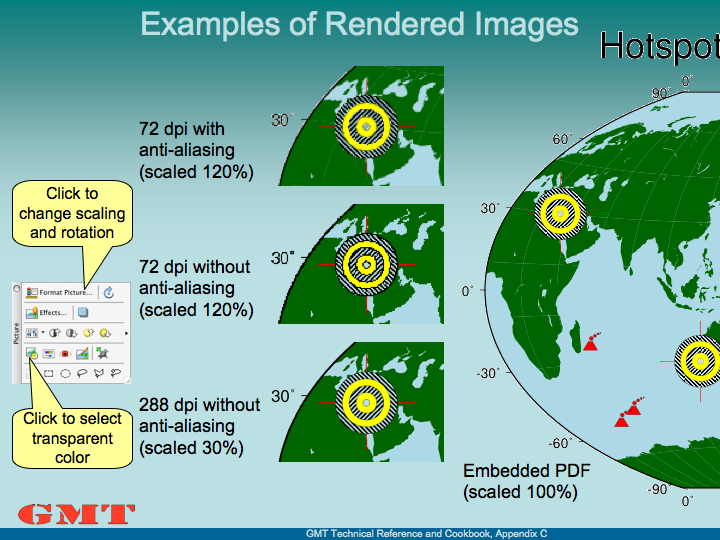
\includegraphics[width=\textwidth,bb=0 0 720 540]{ppt/rendering.png}
   \caption{Examples of rendered images in a \progname{PowerPoint} presentation.}
   \label{fig:rendering}
\end{figure}
\begin{figure}[b]
   \centering
   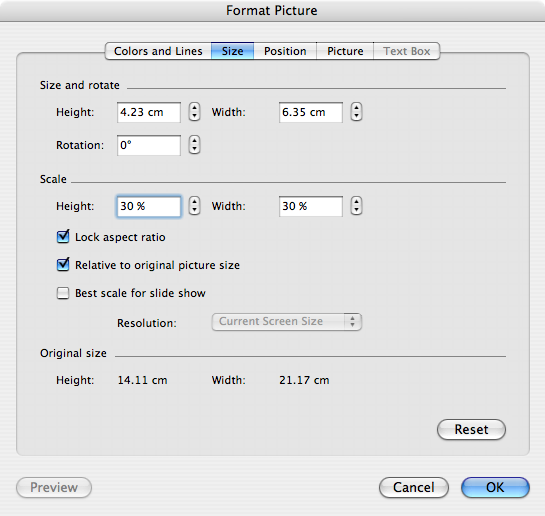
\includegraphics[width=0.6\textwidth,bb=0 0 545 516]{ppt/formatpicture.png}
   \caption{\progname{PowerPoint}'s ``Format Picture'' dialogue to set scale and rotation.}
   \label{fig:formatpicture}
\end{figure}

In Figure~\ref{fig:rendering} we have attempted to include Figure~\ref{fig:GMT_example_20} into a \progname{PowerPoint} presentation. First the \PS\ file was converted to PDF (using \GMTprog{ps2raster}), then loaded into \progname{PowerPoint} and the white background color was made transparent using the formatting toolbar (shown on the left side of Figure~\ref{fig:rendering}). Clearly, when we let \progname{PowerPoint} do the rendering, we do not get the best result:
\begin{enumerate}
\item The anti-aliasing causes the tiles that make up the land to stand out. This is because the anti-aliasing algorithm blurs all edges, even when the tiles join seamlessly.
\item The background color was assumed to be white, hence the text is ``smoothed'' using gray shades. Instead, shades of blue which would be appropriate for the background we are using.
\end{enumerate}

On the central column of Figure~\ref{fig:rendering} we have included PNG versions of a portion of the same example. This shows the workings of anti-aliasing and different resolutions. All samples were obtained with \progname{convert}. The one on the top uses all default settings, resulting in an anti-aliased image at 72 dpi resolution (very much like the PDF included directly into \progname{PowerPoint}).

Just switching anti-aliasing off (middle) is clearly not an option either. It is true that we got rid of the gray blurring and the seams between the tiles, but without anti-aliasing the image becomes very blocky. The solution is to render the image at a higher resolution (e.g., 300 dpi) without anti-aliasing and then shrink the image to the appropriate size (bottom of the central column in Figure~\ref{fig:rendering}). The scaling, rotation as well as the selection of the transparent color can be accomplished through the ``Formatting'' tool bar and the ``Format Picture'' dialogue box of \progname{PowerPoint} (Figure~\ref{fig:formatpicture}), which can be found by double clicking the included image (or selecting and right-clicking or control-clicking on a one-button mouse).

\section{Concluding remarks}

These examples do not constitute endorsements of the products mentioned above; they only represent our limited experience with adding \PS\ to various types of documents.  For other solutions and further help, please post messages to
\htmladdnormallink{gmt-help@hawaii.edu}{mailto:gmt-help@hawaii.edu}.

%------------------------------------------
%	$Id$
%
%	The GMT Documentation Project
%	Copyright (c) 2000-2011.
%	P. Wessel, W. H. F. Smith, R. Scharroo, and J. Luis
%------------------------------------------
%
\chapter{Availability of \gmt\ and related code}
\label{app:D}
\index{GMT@\GMT!obtaining}
\thispagestyle{headings}

\section{Source distribution}
All the source code, support data, PDF
and HTML versions of all documentation (including \UNIX\
manual pages) can be obtained by anonymous
ftp from several mirror sites.  We also maintain a \GMT\
page on the World Wide Web (http://\GMTSITE);
see this page for installation directions 
which allow for a simplified, automatic install procedure
(for the purchase of CD-R and DVD-R media, see \htmladdnormallink{http://www.geoware-online.com}{http://www.geoware-online.com}.)

The \GMT\ compressed tar archives requires \progname{bzip2} to expand.  If this utility
is not installed on your system, you must obtained it by your system's package manager
or install it separately\footnote{http://www.bzip.org}.
The GMT archives are as follows:

\begin{description}

\item[gmt-\GMTDOCVERSION.tar.bz2] Contains all \GMT\ and supplemental source code needed for compilation, support files
	needed at run-time (cpt files, symbols and \PS\ patterns), and all documentation
	(man pages, Cookbook and Technical Reference, and the tutorial), the data files
	used in the tutorial, and all the shell scripts and support data used in the Cookbook section.

\item[gshhs-\GSHHSVERSION.tar.bz2] Contains all resolutions (full, high, intermediate,
low, and crude) of the GSHHS coastline database.  Required to run \GMT.

\end{description}

\index{netCDF, obtaining}

The netCDF library that makes up the backbone of the grid file
i/o operations can be obtained from Unidata by downloading he file
\filename{netcdf.tar.Z} from the anonymous FTP directory of
\underline{unidata.ucar.edu}.

\index{GMT@\GMT!subversion install}
\section{Install via subversion}

The \GMT\ development tree can be installed via subversion.  Simply run
\begin{verbatim}
	svn checkout svn://gmtserver.soest.hawaii.edu/gmt5
\end{verbatim}

\index{GMT@\GMT!binaries for Win32}
\section{Pre-compiled Executables}

For Windows users who just want executables we have three Windows installers available.  Choose one
of the first two and \emph{optionally} the third:

\begin{description}

\item[gmt-\GMTDOCVERSION\_install32.exe] The 32-bit install with all \GMT\ executables (including supplements),
the netCDF DLL, the complete set of GSHHS coastlines, rivers, and borders, the example batch scripts and data, and all documentation in HTML format.

\item[gmt-\GMTDOCVERSION\_install64.exe] The 64-bit install with all \GMT\ executables (including supplements),
the netCDF DLL, the complete set of GSHHS coastlines, rivers, and borders, the example batch scripts and data, and all documentation in HTML format.

\item[gmt-\GMTDOCVERSION\_pdf\_install.exe] Installer for the optional \GMT\ documentation in PDF format.

\end{description}
Usually, only one of the 32- or 64-bit installers will be needed.


%------------------------------------------
%       $Id: GMT_Appendix_E.tex,v 1.9 2005-12-17 05:59:21 pwessel Exp $
%
%       The GMT Documentation Project
%       Copyright 2000-2006.
%       Paul Wessel and Walter H. F. Smith
%------------------------------------------
%
\chapter{Predefined bit and hachure patterns in \gmt}
\label{app:E}
\index{Attributes!fill!pattern}
\index{Fill!attributes!pattern}
\index{Pattern}
\thispagestyle{headings}

\GMT\ provides 90 different bit and hachure patterns that can be
selected with the \Opt{Gp} or \Opt{GP} option in most plotting programs.
The left side of each image was created using \Opt{Gp}, the right side
shows the inverted version using \Opt{GP}.
These patterns are reproduced below at 300 dpi.

\begin{center}
%\epsfig{figure=eps/GMT_App_E.eps}
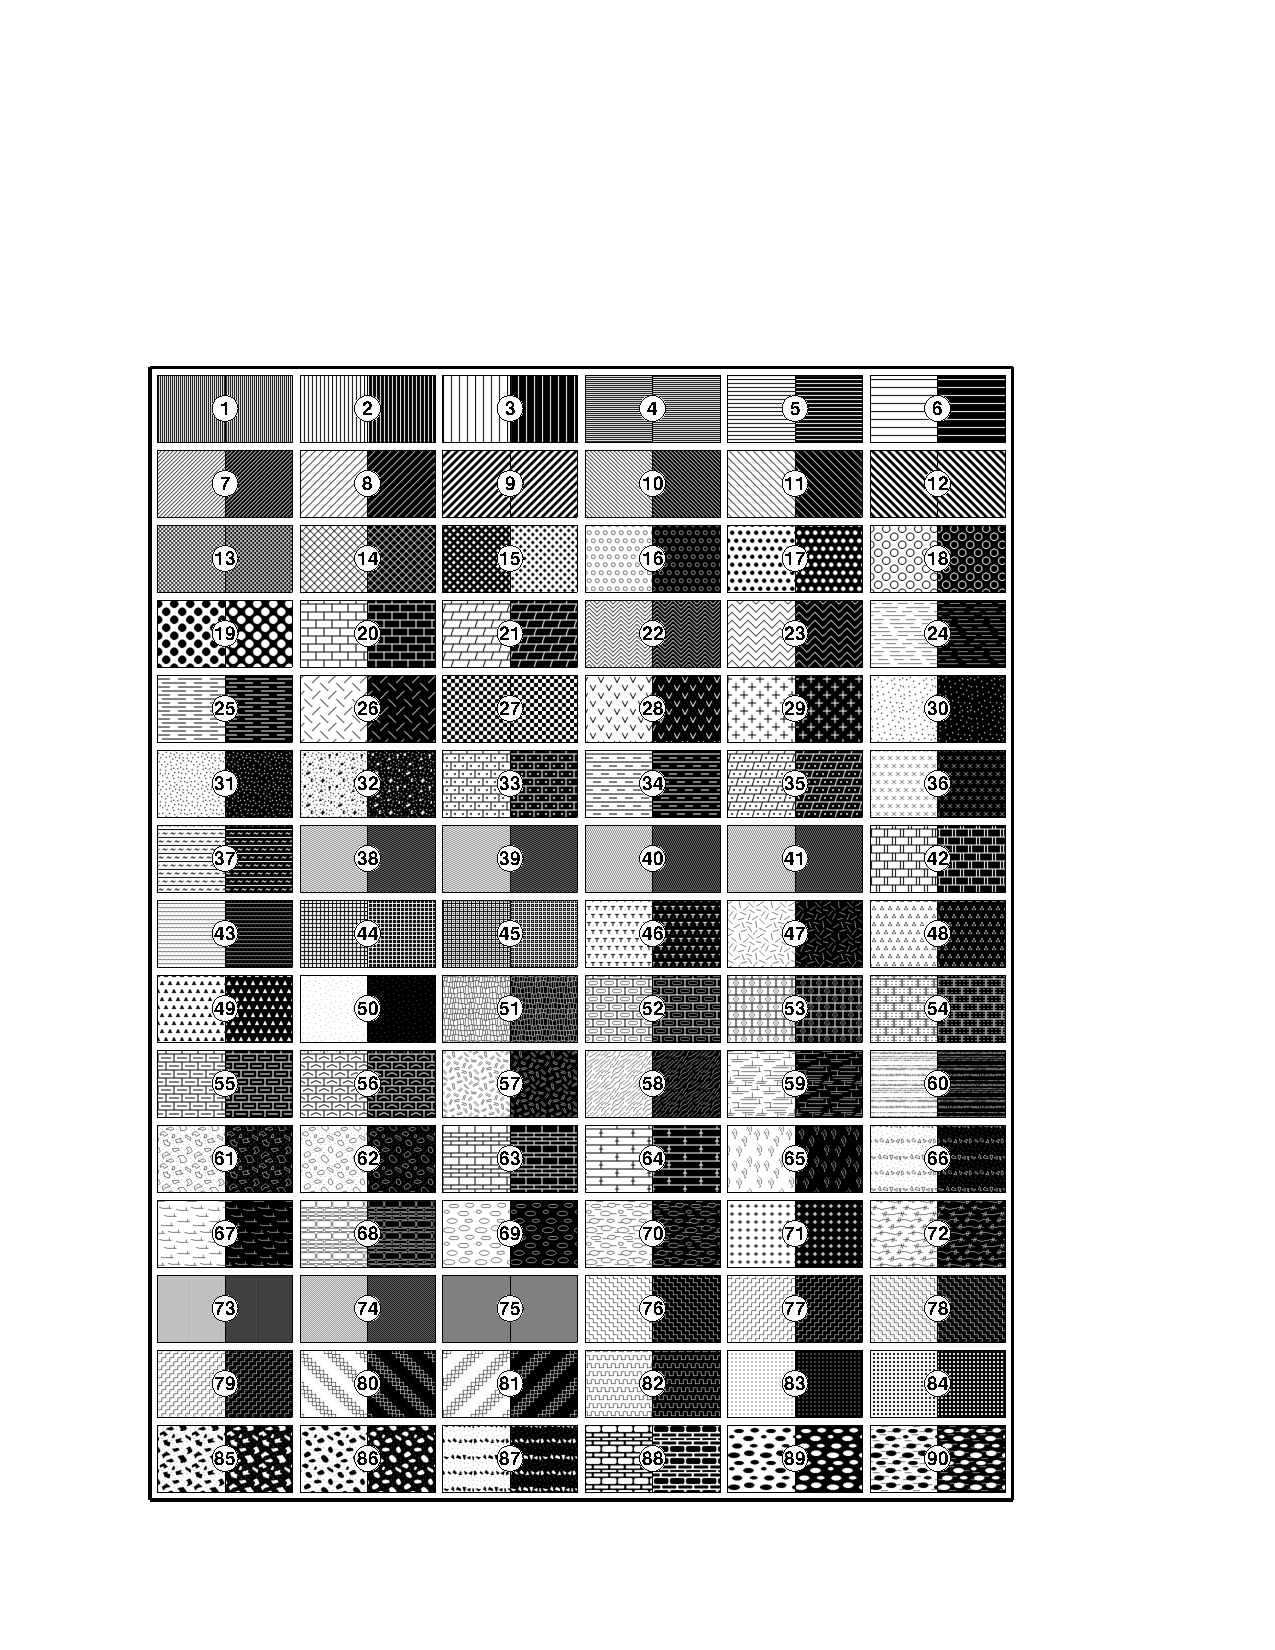
\includegraphics{eps/GMT_App_E}
\end{center}

%------------------------------------------
%	$Id: GMT_Appendix_F.tex,v 1.4 2003-01-14 02:38:03 pwessel Exp $
%
%	The GMT Documentation Project
%	Copyright 2000-2003.
%	Paul Wessel and Walter H. F. Smith
%------------------------------------------
%
\chapter{Chart of octal codes for characters}
\index{Characters!octal}
\index{Octal characters}
\thispagestyle{headings}

\GMTfig[h]{GMT_App_F_stand+}{Octal codes and corresponding symbols for StandardEncoding fonts}

The characters and their octal codes in the Standard encoded fonts
are shown in Figure~\ref{fig:GMT_App_F_stand+}, while the characters and their octal codes in the ISOLatin1
encoded fonts are shown in Figure~\ref{fig:GMT_App_F_iso+}.   Dark gray areas signify codes reserved for
control characters.  In order to use all the extended characters (shown in the light gray boxes) you need to
set {\bf CHAR\_ENCODING} to Standard+ or ISOLatin1+ in your \filename{.gmtdefaults} file\footnote{If you chose
SI units during the installation then the default encoding is ISOLatin1+, otherwise it is Standard+.}.
The chart for the Symbol (\GMT\ font number 12) character
sets are presented in Figure~\ref{fig:GMT_App_F_symbol} below. The octal code is obtained by appending the
column value to the $\backslash$?? value, e.g., $\partial$ is
$\backslash$266 in the Symbol font.  The euro currency symbol is $\backslash$240 in the Symbol font and will
print if your printer supports it (older printer's firmware will not know about the euro).

\GMTfig[h]{GMT_App_F_iso+}{Octal codes and corresponding symbols for ISOLatin1Encoding fonts}

\index{Symbol font}
\index{Font!symbol}

\GMTfig[h]{GMT_App_F_symbol}{Octal codes and corresponding symbols for the Symbol font}

The Pifont ZapfDingbats is available as \GMT\ font number 34 and
can be used for special symbols not listed above.  The various
symbols are illustrated in Figure~\ref{fig:GMT_App_F_dingbats}.

\GMTfig[h]{GMT_App_F_dingbats}{Octal codes and corresponding symbols for ZapfDingbats font}

%------------------------------------------
%	$Id: GMT_Appendix_G.tex,v 1.13 2008-01-23 03:22:47 guru Exp $
%
%	The GMT Documentation Project
%	Copyright 2000-2008.
%	Paul Wessel and Walter H. F. Smith
%------------------------------------------
%
\chapter{\PS\ fonts used by \gmt}
\label{app:G}
\index{Font!standard}
\thispagestyle{headings}

\GMT\ uses the standard 35 fonts that come with most
\PS\ laserwriters.  If your printer does not support
some of these fonts, it will automatically substitute the
default font (which is usually Courier).  The following is
a list of the \GMT\ fonts: \\ 

\GMTfig[h]{GMT_App_G}{The standard 35 \PS\ fonts recognized by \gmt.}

For the special fonts Symbol (12) and ZapfDingbats (34), see the
octal charts in Appendix~F.  When specifying fonts in \GMT, you can
either give the entire font name \emph{or} just the font number listed in
this table.  To change the fonts used in plotting basemap frames, see the man
page for \GMTprog{gmtdefaults}.  For direct plotting of text-strings,
see the man page for \GMTprog{pstext}.  To add additional fonts that you
may have purchased or that are available at your institution, see instructions
in the \filename{CUSTOM\_font\_info.d} under the \filename{share/pslib} directory.

%------------------------------------------
%	$Id$
%
%	The GMT Documentation Project
%	Copyright (c) 2000-2012.
%	P. Wessel, W. H. F. Smith, R. Scharroo, J. Luis and F. Wobbe
%------------------------------------------
%
\chapter{Problems with display of \gmt\ \PS}
\label{app:H}
\thispagestyle{headings}

\GMT\ creates valid (so far as we know) Adobe \PS\
Level 2.  It does not use operators specific to Level 3 and
should therefore produce output that should print on all \PS\ printers\footnote{Note, however, that the \Opt{Q} option in \GMTprog{grdimage}
will exercise a \PS\ Level 3 feature called colormasking.}.  Sometimes unexpected things
happen when \GMT\ output is sent to certain printers or displays.
This section lists some things we have learned from experience,
and some work-arounds.  Note that many of these lessons are now rather old so hopefully
these workarounds no longer apply to anybody...

\section{\PS\ driver bugs}
\index{PostScript@\PS!driver bugs}

When you try to display a \PS\ file on a device,
such as a printer or your screen, then a program called a
\PS\ device driver has to compute which device
pixels should receive which colors (black or white in the case
of a simple laser printer) in order to display the file.  At
this stage, certain device-dependent things may happen.  These
are not limitations of \GMT\ or \PS, but of the
particular display device.  The following bugs are known to us
based on our experiences:

\begin{enumerate}
\index{PostScript@\PS!Sun SPARCprinter bug}

\item 	Early versions of the Sun SPARCprinter software
caused linewidth-dependent path displacement.  We reported
this bug and it has been fixed in newer versions of the software.
Try using \GMTprog{psxy} to draw $y = f(x)$ twice, once with a
thin pen (\Opt{W}1) and once with a fat pen (\Opt{W}10);
if they do not plot on top of each other, you have this kind
of bug and need new software.  The problem may also show up
when you plot a mixture of solid and dashed (or dotted) lines
of various pen thickness

\index{PostScript@\PS!HP Laserjet 4M bug}

\item The first version of the HP Laserjet 4M (prior to Aug--93)
had bugs in the driver program.  The old one was
\PS\ SIMM, part number C2080-60001; the new one
is called \PS\ SIMM, part number C2080-60002.
You need to get this one plugged into your printer if you have
an HP LaserJet 4M.

\index{PostScript@\PS!limitations|(}

\item Apple Laserwriters with the older versions of Apple's
\PS\ driver will give the error ``limitcheck''
and fail to plot when they encounter a path exceeding about
1000--1500 points.  Try to get a newer driver from Apple, but
if you can't do that, set the parameter MAX\_L1\_PATH to
1000--1500 or even smaller in the file \filename{src/pslib\_inc.h}
and recompile \GMT.  The number of points in a \PS\
path can be arbitrarily large, in principle; \GMT\ will only
create paths longer than MAX\_L1\_PATH if the path represents
a filled polygon or clipping path.  Line-drawings (no fill)
will be split so that no segment exceeds MAX\_L1\_PATH.
This means \GMTprog{psxy} \Opt{G} will issue a warning when you
plot a polygon with more than MAX\_L1\_PATH points in it.  It is
then your responsibility to split the large polygon into several
smaller segments.  If \GMTprog{pscoast} gives such warnings and the
file fails to plot you may have to select one of the lower
resolution databases  The path limitation exemplified by these
Apple printers is what makes the higher-resolution coastlines
for \GMTprog{pscoast} non-trivial:  such coastlines have to be
organized so that fill operations do not generate excessively
large paths.  Some HP \PS\ cartridges for the
Laserjet III also have trouble with paths exceeding 1500
points; they may successfully print the file, but it can take
all night!
\index{PostScript@\PS!limitations|)}

\index{PostScript@\PS!Sun pageview}

\item 8-bit color screen displays (and programs which use only
8-bits, even on 24-bit monitors, such as Sun's \progname{pageview} under
OpenWindows) may not dither cleverly, and so the color they show you
may not resemble the color your \PS\ file is asking
for.  Therefore, if you choose colors you like on the screen,
you may be surprised to find that your plot looks different on
the hardcopy printer or film writer.  The only thing you can
do is be aware of this, and make some test cases on your hardcopy
devices and compare them with the screen, until you get used
to this effect.  (Each hardcopy device is also a little
different, and so you will eventually find that you want to
tune your color choices for each device.)  The rgb color cube
in example 11 may help.

\item Some versions of Sun's OpenWindows program \progname{pageview}
have only a limited number of colors available; the number
can be increased somewhat by starting \progname{openwin} with the
option ``\texttt{openwin -cubesize large}''.

\item Finally, \progname{pageview} seem to have problems understanding
the \texttt{setpagedevice} operator.  We recommend you only use
\progname{pageview} on EPS files or use \progname{ghostview} instead.

\index{PostScript@\PS!CMYK and RGB|(}

\item Many color hardcopy devices use CMYK color systems. \GMT\
\PS\ uses RGB (even if your CPT files are using HSV).
The three coordinates of RGB space can be mapped into three
coordinates in CMY space, and in theory K (black) is superfluous.
But it is hard to get CMY inks to mix into a good black or gray,
so these printers supply a black ink as well, hence CMYK.  The
\PS\ driver for a CMYK printer should be smart
enough to compute what portion of CMY can be drawn in K, and
use K for this and remove it from CMY; however, some of them
aren't.

\item In early releases of \GMT\ we always used the \PS\
command \texttt{r g b setrgbcolor} to specify colors, even if the color
happened to be a shade of gray ($r=g=b$) or black ($r=g=b=0$).  One
of our users found that black came out muddy brown when he used
\progname{FreedomOfPress} to make a Versatec plot of a \GMT\ map.
He found that if he used the \PS\ command \texttt{g setgray} (where $g$
is a graylevel) then the problem went away.
Apparently, his installation of \progname{FreedomOfPress} uses only CMY with
the command \texttt{setrgbcolor}, and so \texttt{0 0 0 setrgbcolor}
tries to make black out of CMY instead of K.  To fix this, in
release 2.1 of \GMT\ we changed some routines in \filename{pslib.c}
to check if ($r=g$ and $r=b$), in which case \texttt{g setgray} is
used instead of \texttt{r g b setrgbcolor}.

\item Recent experience with some Tektronix Phaser printers and
with commercial printing shops has shown that this substitution
creates problems precisely opposite of the problems our Versatec
user has.  The Tektronix and commercial (we think it was a Scitex)
machines do not use K when you say \texttt{0 setgray} but they do when
you say \texttt{0 0 0 setrgbcolor}.  We believe that these problems are
likely to disappear as the various software developers make their
codes more robust.  Note that this is not a fault with \GMT:
$r = g = b = 0$ means black and should plot that way.
Thus, the \GMT\ source code as shipped to you checks whether $r=g$
and $r=b$, in which case it uses \texttt{setgray}, else \texttt{setrgbcolor}.
If your gray tones are not being drawn with K, you have two
work-around options: (1) edit the source for \filename{pslib.c}
or (2) edit your \PS\ file and try using \texttt{setrgbcolor}
in all cases.  The simplest way to do so is to redefine the
\texttt{setgray} operator to use \texttt{setrgbcolor}.
Insert the line \\

\indent \texttt{/setgray  \{dup dup setrgbcolor\} def} \\

immediately following the first line in the file (starts with
\%!PS.) 

\item Some color film writers are very sensitive to the brand
of film.  If black doesn't look black on your color slides, try
a different film.
\index{PostScript@\PS!CMYK and RGB|)}

\end{enumerate}

\section{European characters}
\index{Text!European}
\index{Characters!European}
Note for users of \progname{pageview} in Sun OpenWindows: \GMT\ now
offers some octal escape sequences to load European alphabet
characters in text strings (see Section~\ref{sec:escape}).  When
this feature is enabled, the header on \GMT\ \PS\ output includes
a section defining special fonts.  The definition is added to
the header whether or not your plot actually uses the fonts.

Users who view their \GMT\ \PS\ output using
\progname{pageview} in OpenWindows on Sun computers or user older
laserwriters may have difficulties with the European font
definition.  If your installation of OpenWindows followed
a space-saving suggestion of Sun, you may have excluded the
European fonts, in which case \progname{pageview} will fail
to render your plot.

Ask your system administrator about this, or run this simple
test: (1) View a \GMT\ \PS\ file with \progname{pageview}.
If it comes up OK, you will be fine.  If it comes up blank,
open the ``Edit PostScript'' button and examine the lower
window for error messages.  (The European font problem generates
lots of error messages in this window).  (2)  Verify that the
\PS\ file is OK, by sending it to a laserwriter
and making sure it comes out.  (3)  If the \PS\
file is OK but it chokes \progname{pageview}, then edit the \PS\
file, cutting out everything between the lines: \\

\noindent
\%\%\%\%\% START OF EUROPEAN FONT DEFINITION \%\%\%\%\% \\
$<$bunch of definitions$>$ \\
\%\%\%\%\% END OF EUROPEAN FONT DEFINITION \%\%\%\%\% \\

Now try \progname{pageview} on the edited version.  If it now comes
up, you have a limited subset of OpenWindows installed.  If
you discover that these fonts cause you trouble, then you can
edit your \filename{gmt.conf} file to set \textbf{PS\_CHAR\_ENCODING} = Standard,
which will suppress the printing of this definition in the
\GMT\ \PS\ header.  You can
make output which will be viewable in \progname{pageview} without
any editing.  However, you would have to reset this to TRUE
before attempting to use European fonts, and then the output will
become un-\progname{pageview}-able again.  If you try to
concatenate segments of \GMT\ \PS\ made with and without the
European fonts enabled, then you may find that you have problems,
either with the definition, or because you ask for something
not defined.

\section{Hints}
\index{PostScript@\PS!\GMT\ hints}

When making images and perspective views of large amounts of
data, the \GMT\ programs can take some time to run, the resulting
\PS\ files can be very large, and the time to display
the plot can be long.  Fine tuning a plot script can take lots
of trial and error.  We recommend using \GMTprog{grdsample} to make
a low resolution version of the data files you are plotting, and
practice with that, so it is faster; when the script is perfect,
use the full-resolution data files.  We often begin building a
script using only \GMTprog{psbasemap} or \GMTprog{pscoast} to get
the various plots oriented correctly on the page; once this works
we replace the \GMTprog{psbasemap} calls with the actually desired
\GMT\ programs.

If you want to make color shaded relief images and you haven't
had much experience with it, here is a good first cut at the
problem:  Set your \textbf{COLOR\_MODEL} to HSV using \GMTprog{gmtset}.  Use
\GMTprog{makecpt} or \GMTprog{grd2cpt} to make a continuous color
palette spanning the range of your data.  Use the \Opt{Nt}
option on \GMTprog{grdgradient}.  Try the result, and then play with
the tuning of the \filename{gmt.conf}, the CPT file, and
the gradient file.

%------------------------------------------
%	$Id$
%
%	The GMT Documentation Project
%	Copyright (c) 2000-2011.
%	P. Wessel, W. H. F. Smith, R. Scharroo, and J. Luis
%------------------------------------------
%
\chapter{Color Space: The final frontier}
\label{app:I}
\thispagestyle{headings}

\index{Color|(}
\index{Color!HSV system|(}
\index{Color!RGB system|(}

In this Appendix, we are going to try to explain the relationship
between the RGB, CMYK, and HSV color systems so as to (hopefully) make
them more intuitive.  \GMT\ allows users to specify colors in CPT
files in either of these three systems. Interpolation between colors is performed in either RGB or HSV, depending on the specification in the CPT file. Below, we will explain why this all matters.

\section{RGB color system}
Remember your (parents') first color television set? Likely it had three little bright colored squares on it: red, green, and blue. And that is exactly what each color on the tube is made of: varying levels of red, green and blue light. Switch all of them off, $r=g=b=0$, then you have black. All of them at maximum, $r=g=b=255$, creates white. Your computer screen works the same way.

A mix of levels of red, green, and blue creates basically any color imaginable. In \GMT\ each color can be represented by the triplet $r$/$g$/$b$. For example, 127/255/0 (half red, full green, and no blue) creates a color called chartreuse. The color sliders in the graphics program \progname{GIMP} are an excellent way to experiment with colors, since they show you in advance how moving one of the color sliders will change the color. As Figure~\ref{fig:gimp}\emph{a} shows: increase the red and you will get a more yellow color, while lowering the blue level will turn it into brown.

\begin{figure}[b]
   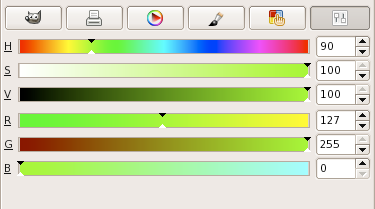
\includegraphics[width=0.47\textwidth,bb=0 0 375 209]{gimp-sliders.png}~\emph{a}\hfill
   \emph{b}~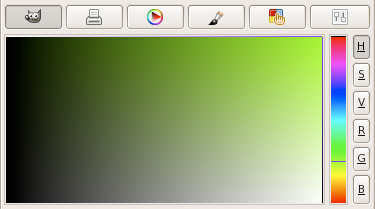
\includegraphics[width=0.47\textwidth,bb=0 0 375 209]{gimp-panel.png}
   \caption{Chartreuse in \protect\progname{GIMP}. (\emph{a}) Sliders indicate how the color is altered when changing the H, S, V, R, G, or B levels. (\emph{b}) For a constant hue (here 90\DS) value increases to the right and saturation increases up, so the ``pure'' color is on the top right.}
   \label{fig:gimp}
\end{figure}

Is chocolate your favorite color, but you do not know the RGB equivalent values? Then look them up in Figure~\ref{fig:RGBchart} or type \progname{man gmtcolors} for a full list. It's 210/105/30. But \GMT\ makes it easy on you: you can specify pen, fill, and palette colors by any of the more than 500 unique colors found in that file.

Are you very web-savvy and work best with hexadecimal color codes as they are used in HTML? Even that is allowed in \GMT. Just start with a hash mark (\texttt{\#}) and follow with the 2 hexadecimal characters for red, green, and blue. For example, you can use \texttt{\#79ff00} for chartreuse, \texttt{\#D2691E} for chocolate.

\begin{figure}
   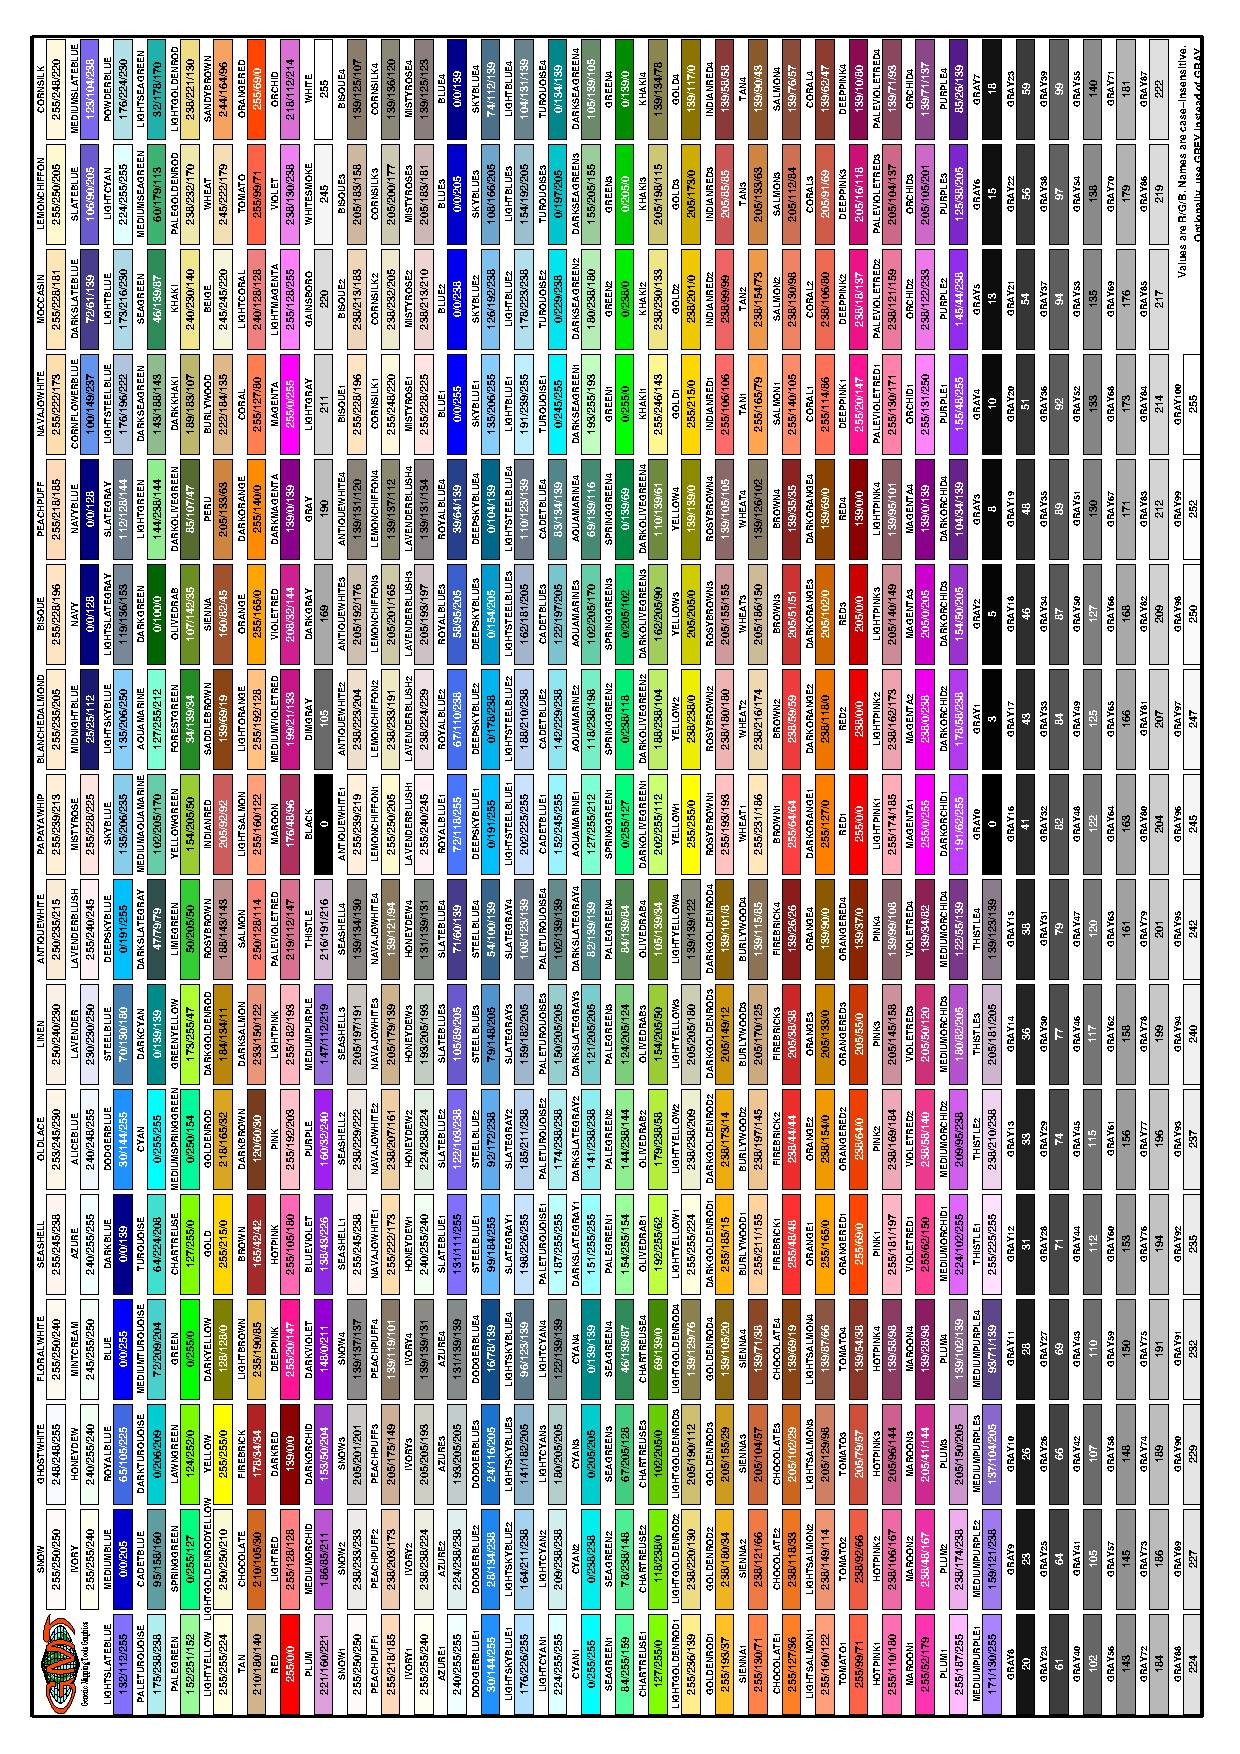
\includegraphics[angle=90,width=\textwidth]{GMT_RGBchart_a4}
   \caption{The 555 unique color names that can be used in GMT. Lower, upper, or mixed cases, as well as the british
   spelling of ``grey'' are allowed. A4, Letter, and Tabloid sized versions of this RGB chart can be found in the
   GMT documentation directory.}
   \label{fig:RGBchart}
\end{figure}

\section{HSV color system}
If you have played around with RGB color sliders, you will have noticed that it is not intuitive to make a chosen color lighter or darker, more saturated or more gray. It would involve changing three sliders. To make it easier to manipulate colors in terms of lightness and saturation, another coordinate system was invented: HSV (hue, saturation, value). Those terms can be made clear best by looking at the color sliders in Figure~\ref{fig:gimp}\emph{a}. Hue (running from 0\DS\ to 360\DS) gives you the full spectrum of saturated colors. Saturation (from 0 to 1, or 100\%) tells you how `full' your color is: reduce it to zero and you only have gray scales. Value (from 0 to 1, or 100\%) will bring you from black to a fully saturated color. Note that ``value'' is not the same as ``intensity'', or ``lightness'', used in other color geometries. ``Brilliance'' may be the best alternative word to describe ``value''. Apple calls it as ``brightness'', and hence refers to HSB for this color space.

Want more chartreuse or chocolate? You can specify them in \GMT\ as 90-1-1 and 25-0.86-0.82, respectively.

\section{The color cube}
We are going to try to give you a geometric picture of color
mixing in RGB and HSV by means of a tour of the RGB cube depicted in Figure~\ref{fig:GMT_example_11}.  The geometric
picture is most helpful, we think, since HSV are not orthogonal
coordinates and not found from RGB by a simple algebraic transformation.
So here goes: Look at the
cube face with black, red, magenta, and blue corners.
This is the $g$ = 0 face.  Orient the cube so that you are
looking at this face with black in the lower left corner.  Now
imagine a right-handed cartesian ($r$,$g$,$b$) coordinate system
with origin at the black point; you are looking at the $g = 0$
plane with $r$ increasing to your right, $g$ increasing
away from you, and $b$ increasing up.  Keep this sense of
($r$,$g$,$b$) as you look at the cube.

Now tip the cube such that the black corner faces down and the white corner up. When looking from the top, you can see the hue, contoured in gray solid lines, running around in 360\DS\ counter-clockwise. It starts with shades of red (0\DS), then goes through green (120\DS) and blue (240\DS), back to red.

On the three faces that are now on the lower side (with the white print) one of ($r$,$g$,$b$) is equal to 0. These three faces meet at the black corner, where $r = g = b = 0$. On these three faces the colors are fully saturated: $s$ = 1. The dashed white lines indicate different levels of $v$, ranging from 0 to 1 with contours every 0.1.

On the upper three faces (with the black print), one of ($r$,$g$,$b$) is equal to the
maximum value.  These three faces meet at the white corner, where
$r = g = b = 255$.  On these three faces value is at
its maximum: $v$ = 1 (or 100\%). The dashed black lines indicate varying levels of saturation: $s$ ranges from 0 to
1 with contours every 0.1.

Now turn the cube around on its vertical axis (running from the black to the white corner). Along the six edges that zigzag around the ``equator'', both saturation and value are maximum, so $s = v = 1$. Twirling the cube around and tracing the zigzag, you will visit six of the eight corners of the
cube, with changing hue ($h$):  red (0\DS), yellow (60\DS), green
(120\DS), cyan (180\DS), blue (240\DS), and magenta
(300\DS). Three of these are the RGB colors; the other three
are the CMY colors which are the complement of RGB and are used in many
color hardcopy devices (see below).  The only cube
corners you did not visit on this path are the black and white corners.
They lie on the vertical axis where hue is undefined and $r = g = b$. Any point on this axis is a shade of gray.

Let us call the points where $s = v = 1$ (points along the RYGCBM path described above) the ``pure'' colors.  If we start at a pure color
and we want to whiten it, we can keep $h$ constant and $v = 1$
while decreasing $s$; this will move us along one of the cube
faces toward the white point.  If we start at a pure color and we want
to blacken it, we can keep $h$ constant and $s = 1$ while decreasing
$v$; this will move us along one of the cube faces toward the black
point.  Any point in ($r$,$g$,$b$) space which can be thought of as a
mixture of pure color + white, or pure color + black, is on a face of
the cube.

The points in the interior of the cube are a little harder to describe.
The definition for $h$ above works at all points in (non-gray)
($r$,$g$,$b$) space, but so far we have only looked at ($s$,
$v$) on the cube faces, not inside it.  At interior points, none
of ($r$,$g$,$b$) is equal to either 0 or 255.  Choose such a point,
not on the gray axis.  Now draw a line through your point so that the
line intersects the gray axis and also intersects the RYGCBM path of
edges somewhere.  It is always possible to construct this line, and
all points on this line have the same hue.  This construction shows
that any point in RGB space can be thought of as a mixture of a pure
color plus a shade of gray.  If we move along this line away from the
gray axis toward the pure color, we are ``purifying'' the color by
``removing gray''; this move increases the color's saturation.  When
we get to the point where we cannot remove any more gray, at least one
of ($r$,$g$,$b$) will have become zero and the color is now fully
saturated; $s = 1$.  Conversely, any point on the gray axis is
completely undersaturated, so that $s = 0$ there.  Now we see that
the black point is special, $s$ is both 0 and 1 at the same time. In other words, at the black point saturation in undefined (and so is hue). The convention is to use $h = s = v = 0$ at this point.

It remains to define value. To do so, try this:
Take your point in RGB space and construct a line through it so that
this line goes through the black point; produce this line from black
past your point until it hits a face on which $v = 1$.  All points
on this line have the same hue.  Note that this line and the line we
made in the previous paragraph are both contained in the plane whose
hue is constant.  These two lines meet at some arbitrary
angle which varies depending on which point you chose.  Thus HSV is
not an orthogonal coordinate system.  If the line you made in the
previous paragraph happened to touch the gray axis at the black point,
then these two lines are the same line, which is why the black point
is special.  Now, the line we made in this paragraph illustrates the
following:  If your chosen point is not already at the end of the
line, where $v = 1$, then it is possible to move along the line in
that direction so as to increase ($r$,$g$,$b$) while keeping the
same hue.  The effect this has on a color monitor is to make the
color more ``brilliant'', your hue will become ``stronger''; if you are already on a plane where
at least one of ($r$,$g$,$b$) = 255, then you cannot get a stronger
version of the same hue.  Thus, $v$ measures brilliance or strength.  Note that
it is not quite true to say that $v$ measures distance away from
the black point, because $v$ is not equal to $\sqrt{r^2 + g^2 + b^2}/255$.

Another representation of the HSV space is the color cone illustrated in Figure~\ref{fig:hsv-cone}.

\begin{figure}[h]
   \parbox[b]{0.54\textwidth}{``Pure'' colors are around the edge of the circular surface at the top. Hue runs counter-clockwise. Saturation decreases to the center. Value increases from zero (black) at the bottom to 1 at the top. Gray shades are along the vertical axis.}%
   \hfill%
   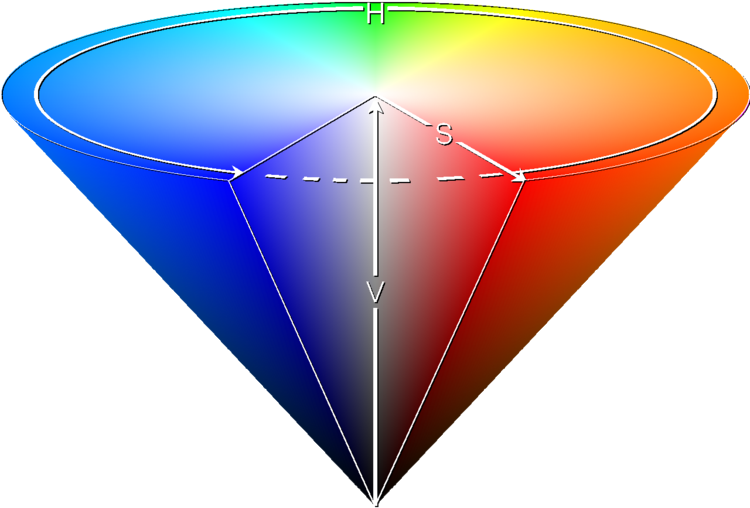
\includegraphics[width=0.45\textwidth,bb=0 0 750 508]{hsv-cone.png}%
   \caption{The HSV color space.}
   \label{fig:hsv-cone}
\end{figure}

\section{Color interpolation}
\index{Color!interpolation}
From studying the RGB cube, we hope you will have understood that there are different routes to follow between two colors, depending whether you are in the RGB or HSV system. Suppose you would make an interpolation between blue and red. In the RGB system you would follow a path diagonally across a face of the cube, from 0/0/255 (blue) via 127/0/127 (purple) to 255/0/0 (red). In the HSV system, you would trace two edges, from 240-1-1 (blue) via 300-1-1 (magenta) to 360-1-1 (red). That is even assuming software would be smart enough to go the shorter route. More likely, red will be recorded as 0-1-1, so hue will be interpolated the other way around, reducing hue from 240\DS\ to 0\DS, via cyan, green, and yellow.

Depending on the design of your color palette, you may want to have it either way. By default, \GMT\ interpolates in RGB space, even when the original color palette is in the HSV system. However, when you add the line \texttt{\#COLOR\_MODEL=+HSV} (with the leading `+' sign) in the header of the color palette file, \GMT\ will not only read the color representation as HSV values, but also interpolate colors in the HSV system. That means that H, S, and V values are interpolated linearly between two colors, instead of their respective R, G, and B values.

The top row in Figure~\ref{fig:GMT_color_interpolate} illustrates two examples: a blue-white-red scale (the \textsf{polar} palette in Appendix~\ref{app:M}) interpolated in RGB and the \textsf{rainbow} palette interpolated in HSV. The bottom row of the Figure demonstrates how things can go terribly wrong when you do the interpolation in the other system.

\begin{figure}[h]
   \centering
   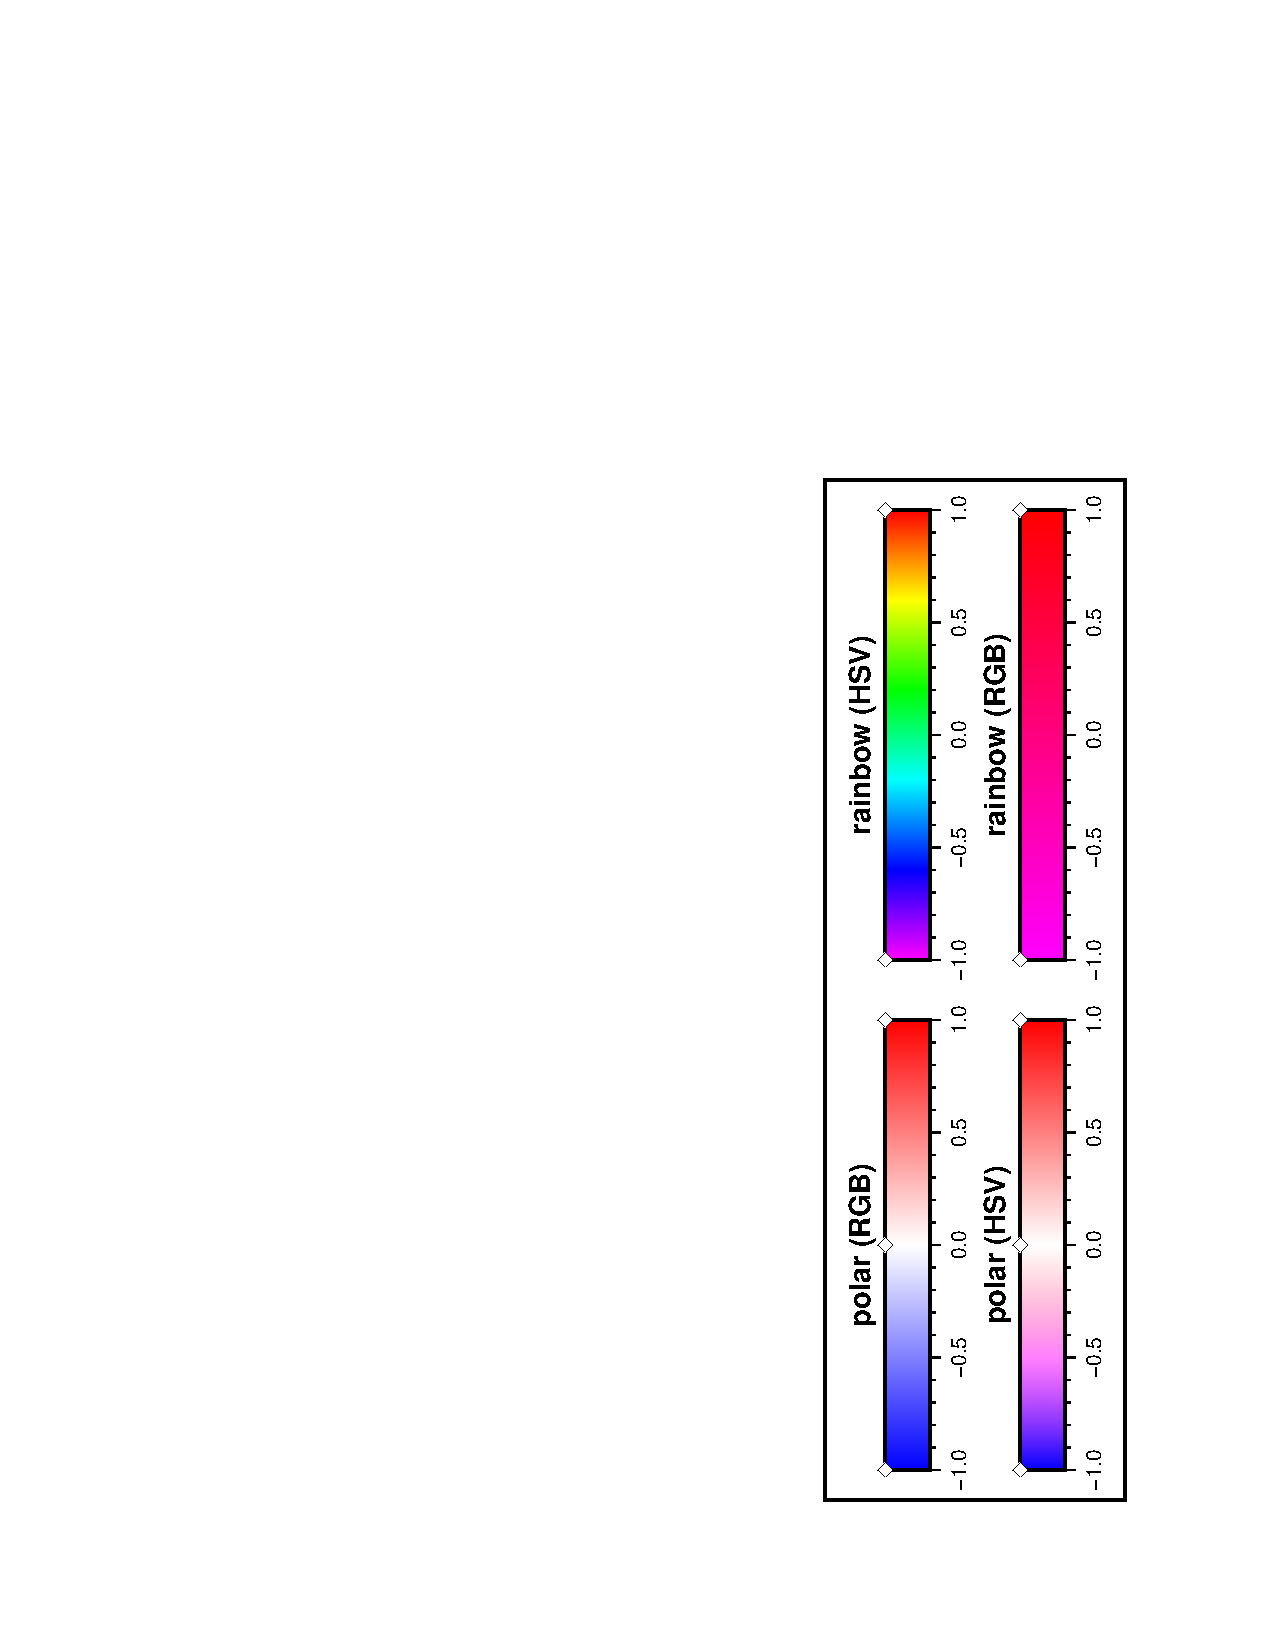
\includegraphics[width=0.80\textwidth]{GMT_color_interpolate}%
   \caption{When interpolating colors, the color system matters. The polar palette on the left needs to be interpolated in RGB, otherwise hue will change between blue (240\DS) and white (0\DS). The rainbow palette should be interpolated in HSV, since only hue should change between magenta (300\DS) and red (0\DS). Diamonds indicate which colors are defined in the palettes; they are fixed, the rest is interpolated.}
   \label{fig:GMT_color_interpolate}
\end{figure}

\section{Artificial illumination}
\index{Illumination, artificial}
\index{Artificial illumination}
\GMT\ uses the HSV system to
achieve artificial illumination of colored images (e.g. \Opt{I}
option in \GMTprog{grdimage}) by changing the saturation \emph{s} and value \emph{v}
coordinates of the color.  When the intensity is zero (flat illumination), the data
are colored according to the CPT file.  If the intensity is
non-zero, the color is either lightened or darkened depending on the illumination.
The color is first converted to HSV (if necessary) and then
darkened by moving ($s$,$v$) toward (\textbf{COLOR\_HSV\_MIN\_S},
\textbf{COLOR\_HSV\_MIN\_V}) if the intensity is negative, or lightened by sliding ($s$,$v$) toward
(\textbf{COLOR\_HSV\_MAX\_S}, \textbf{COLOR\_HSV\_MAX\_V}) if the illumination is positive.
The extremes of the $s$ and $v$ are defined in the \filename{gmt.conf} file and are usually
chosen so the corresponding points are nearly black ($s$ = 1,
$v$ = 0) and white ($s$ = 0, $v$ = 1).
The reason this works is that the HSV system allows movements in
color space which correspond more closely to what we mean by
``tint'' and ``shade''; an instruction like ``add white'' is
easy in HSV and not so obvious in RGB.

\section{Thinking in RGB or HSV}
The RGB system is understandable because it is cartesian, and we all
learned cartesian coordinates in school.  But it doesn't help us
create a tint or shade of a color; we cannot say, ``We want orange,
and a lighter shade of orange, or a less vivid orange''.  With HSV we
can do this, by saying, ``Orange must be between red and yellow, so
its hue is about $h$ = 30\DS; a less vivid orange has a lesser
$s$, a darker orange has a lesser $v$''.  On the other hand,
the HSV system is a peculiar geometric construction, more like a cone (Figure~\ref{fig:hsv-cone}). It is not an
orthogonal coordinate system, and it is not found by a matrix
transformation of RGB; these make it difficult in some cases too.
Note that a move toward black or a move toward white will change both
$s$ and $v$, in the general case of an interior point in the
cube. The HSV system also doesn't behave well for very dark colors,
where the gray point is near black and the two lines we constructed
above are almost parallel.  If you are trying to create nice colors
for drawing chocolates, for example, you may be better off guessing
in RGB coordinates.
\index{Color!HSV system|)}
\index{Color!RGB system|)}

\section{CMYK color system}
\index{Color!CMYK system}
Finally, you can imagine that printers work in a different way: they mix different paints to make a color. The more paint, the darker the color, which is the reverse of adding more light. Also, mixing more colored paints does not give you true black, so that means that you really need four colors to do it right. Open up your color printer and you'll probably find four cartridges: cyan, magenta, yellow (often these are combined into one), and black. They form the CMYK system of colors, each value running from 0 to 1 (or 100\%). In \GMT\ CMYK color coding can be achieved using $c$/$m$/$y$/$k$ quadruplets.

Obviously, there is no unique way to go from the 3-dimensional RGB system to the 4-dimensional CMYK system. So, again, there is a lot of hand waving applied in the transformation. Strikingly, CMYK actually covers a smaller color space than RGB. We will not try to explain you the details behind it, just know that there is a transformation needed to go from the colors on your screen to the colors on your printer. It might explain why what you see is not necessarily what you get. If you are really concerned about how your color plots will show up in your PhD thesis, for example, it might be worth trying to save and print all your color plots using the CMYK system. Letting \GMT\ do the conversion to CMYK may avoid
some nasty surprises when it comes down to printing. To specify the color space of your \PS\ file, set \textbf{PS\_COLOR\_MODEL}
in the \filename{gmt.conf} file to RGB, HSV, or CMYK.
\index{Color|)}

%------------------------------------------
%	$Id: GMT_Appendix_J.tex,v 1.7 2005-07-12 04:13:24 pwessel Exp $
%
%	The GMT Documentation Project
%	Copyright 2000-2005.
%	Paul Wessel and Walter H. F. Smith
%------------------------------------------
%
\chapter{Filtering of data in \gmt}
\thispagestyle{headings}

The \GMT\ programs \GMTprog{filter1d} (for tables of data indexed
to one independent variable) and \GMTprog{grdfilter} (for data
given as 2-dimensional grids) allow filtering of data by a
moving-window process.  (To filter a grid by Fourier transform use
\GMTprog{grdfft}.)  Both programs use an argument
\Opt{F}$<${\it type}$><${\it width}$>$ to specify the type of
process and the window's width (in 1-d) or diameter (in 2-d).
(In \GMTprog{filter1d} the width is a length of the time or
space ordinate axis, while in \GMTprog{grdfilter} it is the
diameter of a circular area whose distance unit is related to
the grid mesh via the \Opt{D} option). If the process is a
median or mode estimator then the window 
output cannot be written as a convolution and the filtering
operation is not a linear operator.  If the process is a weighted
average, as in the boxcar, cosine, and gaussian filter types, 
then linear operator theory applies to the filtering process.
These three filters can be described as convolutions with an
impulse response function, and their transfer functions 
can be used to describe how they alter components in the input
as a function of wavelength.

Impulse responses are shown here for the boxcar, cosine, and
gaussian filters.  Only the relative amplitudes of the filter
weights shown; the values in the center of the window have 
been fixed equal to 1 for ease of plotting.  In this way the
same graph can serve to illustrate both the 1-d and 2-d impulse
responses; in the 2-d case this plot is a diametrical
cross-section through the filter weights (Figure~\ref{fig:GMT_App_J_1}).

\GMTfig[H]{GMT_App_J_1}{Impulse responses for \gmt\ filters.}

Although the impulse responses look the same in 1-d and 2-d,
this is not true of the transfer functions; in 1-d the transfer
function is the Fourier transform of the impulse response, 
while in 2-d it is the Hankel transform of the impulse response.
These are shown in Figures~\ref{fig:GMT_App_J_2} and
\ref{fig:GMT_App_J_3}, respectively.  Note that in 1-d the boxcar transfer
function has its first zero crossing at $f = 1$, while in 2-d 
it is around $f \sim 1.2$.  The 1-d cosine transfer function
has its first zero crossing at $f = 2$; so a cosine filter needs
to be twice as wide as a boxcar filter in order to zero the same
lowest frequency.  As a general rule, the cosine and gaussian
filters are ``better'' in the sense that they do not have the
``side lobes'' (large-amplitude oscillations in the transfer
function) that the boxcar filter has.  However, they are
correspondingly ``worse'' in the sense that they require more
work (doubling the width to achieve the same cut-off wavelength).

\clearpage

\GMTfig[H]{GMT_App_J_2}{Transfer functions for 1-D \gmt\ filters.}

One of the nice things about the gaussian filter is that its
transfer functions are the same in 1-d and 2-d.  Another nice
property is that it has no negative side lobes.  There are many 
definitions of the gaussian filter in the literature (see page
7 of Bracewell\footnote{R. Bracewell, \emph{The Fourier Transform
and its Applications}, McGraw-Hill, London, 444p., 1965.}).  We
define $\sigma$ equal to 1/6 of the filter width, and the impulse
response proportional to $\exp[-0.5(t/\sigma)^2)$.  With this
definition, the transfer function is $\exp[-2(\pi\sigma f)^2]$
and the wavelength at which the transfer function equals 0.5 is 
about 5.34 $\sigma$, or about 0.89 of the filter width.

\GMTfig[H]{GMT_App_J_3}{Transfer functions for 2-D (radial) \gmt\ filters.}

%------------------------------------------
%	$Id: GMT_Appendix_K.tex,v 1.5 2004-01-02 22:45:12 pwessel Exp $
%
%	The GMT Documentation Project
%	Copyright 2000-2004.
%	Paul Wessel and Walter H. F. Smith
%------------------------------------------
%
\chapter{The \gmt\ High-Resolution Coastline Data}
\index{GMT@\GMT!coastlines|(}
\index{Coastlines!preprocessing|(}
\thispagestyle{headings}

Starting with version 3.0, \GMT\ use a completely new coastline
database and the \GMTprog{pscoast} utility was been completely
rewritten to handle the new file format.  Many users have asked
us why it has taken so long for \GMT\ to use a high-resolution
coastline database; after all, such data have been available in
the public domain for years.  To answer such questions we will
take you along the road that starts with these public domain
data sets and ends up with the database used by \GMT.

\section{Selecting the right data} 
\index{World Data Bank II}
\index{CIA Data Bank}
\index{World Vector Shoreline}
\index{WVS}
\index{WDB}

There are two well-known public-domain data sets that could be
used for this purpose.  Once is known as the World Data Bank II
or CIA Data Bank (WDB) and contains coastlines, lakes, political
boundaries, and rivers.  The other, the World Vector Shoreline
(WVS) only contains shorelines between saltwater and land (i.e.,
no lakes).  It turns out that the WVS data is far superior to the
WDB data as far as data quality goes, but as noted it lacks lakes,
not to mention rivers and borders.  We decided to use the WVS
whenever possible and supplement it with WDB data.  We got these
data over the Internet; they are also available on CD-ROM from
the National Geophysical Data Center in Boulder, Colorado\footnote{
www.ngdc.noaa.gov}.

\section{Format required by \gmt} 

In order to paint continents or oceans it is necessary that the
coastline data be organized in polygons that may be filled.
Simple line segments can be used to draw the coastline, but for
painting polygons are required.  Both the WVS and WDB data
consists of unsorted line segments: there is no information
included that tells you which segments belong to the same
polygon (e.g., Australia should be one large polygon).
In addition, polygons enclosing land must be differentiated from
polygons enclosing lakes since they will need different paint.
Finally, we want \GMTprog{pscoast} to be flexible enough that it can
paint the land \emph{or} the oceans \emph{or} both.
If just land (or oceans) is selected we do not want to paint
those areas that are not land (or oceans) since previous plot
programs may have drawn in those areas.  Thus, we will need to
combine polygons into new polygons that lend themselves to fill
land (or oceans) only (Note that older versions of \GMTprog{pscoast}
always painted lakes and wiped out whatever was plotted beneath).

\section{The long and winding road} 

The WVS and WDB together represent more than 100 Mb of binary
data and something like 20 million data points.  Hence, it
becomes obvious that any manipulation of these data must be
automated.  For instance, the reasonable requirement that no
coastline should cross another coastline becomes a complicated
processing step.

\begin{enumerate} 

\item To begin, we first made sure that all data were ``clean'',
i.e. that there were no outliers and bad points.  We had to
write several programs to ensure data consistency and remove
``spikes'' and bad points from the raw data.  Also, crossing
segments were automatically ``trimmed'' provided only
a few points had to be deleted.  A few hundred more complicated
cases had to be examined semi-manually.

\item Programs were written to examine all the loose segments
and determine which segments should be joined to produce
polygons.  Because not all segments joined exactly (there were
non-zero gaps between some segments) we had to find all possible
combinations and choose the simplest combinations.
The WVS segments joined to produce more than 200,000 polygons,
the largest being the Africa-Eurasia polygon which has 1.4
million points.  The WDB data resulted in a smaller data base
($\sim$25\% of WVS).

\item We now needed to combine the WVS and WDB data bases.
The main problem here is that we have duplicates of polygons:
most of the features in WVS are also in WDB.  However, because
the resolution of the data differ it is nontrivial to figure
out which polygons in WDB to include and which ones to ignore.
We used two techniques to address this problem.
First, we looked for crossovers between all possible pairs of
polygons.  Because of the crossover processing in step 1 above we know
that there are no remaining crossovers within WVS and WDB; thus
any crossovers would be between WVS and WDB polygons.  Crossovers
could mean two things: (1) A slightly misplaced WDB polygon
crosses a more accurate WVS polygon, both representing the same
geographic feature, or (2) a misplaced WDB polygon (e.g. a small
coastal lake) crosses the accurate WVS shoreline.  We distinguished
between these cases by comparing the area and centroid of the two
polygons.  In almost all cases it was obvious when we had
duplicates; a few cases had to be checked manually.  Second,
on many occasions the WDB duplicate polygon did not cross its
WVS counterpart but was either entirely inside or outside the
WVS polygon.  In those cases we relied on the area-centroid tests.

\item While the largest polygons were easy to identify by visual
inspection, the majority remain unidentified.  Since it is
important to know whether a polygon is a continent or a small
pond inside an island inside a lake we wrote programs that would
determine the hierarchical level of each polygon.  Here, level~=~1
represents ocean/land boundaries, 2 is land/lakes borders, 3 is
lakes/islands-in-lakes, and 4 is islands-in-lakes/ponds-in-islands-in-lakes.
Level 4 was the highest level encountered in the data.
To automatically determine the hierarchical levels we wrote
programs that would compare all possible pairs of polygons
and find how many polygons a given polygon was inside.  Because
of the size and number of the polygons such programs would
typically run for 3 days on a Sparc-2 workstation.

\item Once we know what type a polygon is we can enforce a
common ``orientation'' for all polygons. We arranged them so
that when you move along a polygon from beginning to end, your
left hand is pointing toward ``land''.  At this step we also
computed the area of all polygons since we would like the
option to plot only features that are bigger than a minimum
area to be specified by the user.

\item Obviously, if you need to make a map of Denmark then
you do not want to read the entire 1.4 million points making
up the Africa-Eurasia polygon.  Furthermore, most plotting
devices will not let you paint and fill a polygon of that size
due to memory restrictions.  Hence, we need to partition the
polygons so that smaller subsets can be accessed rapidly.
Likewise, if you want to plot a world map on a letter-size paper
there is no need to plot 10 million data points as most of them
will plot several times on the same pixel and the operation
would take a very long time to complete.  We chose to make 5
versions on the database, corresponding to different resolutions.
The decimation was carried out using the Douglas-Peucker (DP)
line-reduction algorithm\footnote{Dougles, D.H., and T. K. Peucker,
1973, Algorithms for the reduction of the number of points
required to represent a digitized line or its caricature,
{\it Canadian Cartographer}, 10, 112--122.}.  We chose the
cutoffs so that each subset was approximately 20\% the size of
the next higher resolution.  The five resolutions are called
{\bf f}ull, {\bf h}igh, {\bf i}ntermediate, {\bf l}ow, and
{\bf c}rude; they are accessed in \GMTprog{pscoast}, \GMTprog{gmtselect},
and \GMTprog{grdlandmask} with the \Opt{D} option�\footnote{ The full
and high resolution files are in separate archives because of their
size.  Not all users may need these files as the intermediate data
set is better than the data provided with version 2.1.4.}.  For each of
these 5 data sets ({\bf f}, {\bf h}, {\bf i}, {\bf l}, {\bf c})
we specified an equidistant grid (1\DS, 2\DS, 5\DS,
10\DS, 20\DS) and split all polygons into line-segments
that each fit inside one of the many boxes defined by these grid
lines.  Thus, to paint the entire continent of Australia we
instead paint many smaller polygons made up of these line
segments and gridlines.  Some book-keeping has to be done since
we need to know which parent polygon these smaller pieces came
from in order to prescribe the correct paint or ignore if the
feature is smaller than the cutoff specified by the user.  The
resulting segment coordinates were then scaled to fit in short
integer format to preserve precision and written in netCDF format
for ultimate portability across hardware platforms\footnote{
If you need complete polygons in a simpler format, see the article
on GSHHS\index{GSHHS} (Wessel, P., and W. H. F. Smith, 1996, A Global, self-consistent, hierarchical, high-resolution shoreline database,
{\it J. Geophys. Res. 101}, 8741--8743).}.

\item While we are now back to a file of line-segments we are in
a much better position to create smaller polygons for painting.
Two problems must be overcome to correctly paint an area:

\begin{itemize}

\item We must be able to join line segments and grid cell borders
into meaningful polygons; how we do this will depend on whether
we want to paint the land or the oceans.

\item We want to nest the polygons so that no paint falls on areas
that are ``wet'' (or ``dry''); e.g., if a grid cell completely on
land contains a lake with a small island, we do not want to paint
the lake and then draw the island, but paint the annulus or ``donut''
that is represented by the land and lake, and then plot the island.

\end{itemize}

\GMT\ uses a polygon-assembly routine that carries out these
tasks on the fly.
\index{GMT@\GMT!coastlines|)}
\index{Coastlines!preprocessing|)}

\end{enumerate} 

\section{The Five Resolutions} 

We will demonstrate the power of the new database by starting with
a regional hemisphere map centered near Papua New Guinea and zoom
in on a specified point.  The map regions will be specified in
projected km from the projection center, e.g., we may want the
map to go from \mbox{-2000} km to \mbox{+2000} km in the longitudinal direction
and \mbox{-1500} km to +1500 km in the latitudinal direction.
However, \GMT\ programs expects degrees in the \Opt{R} option that
specifies the desired region.  Given the chosen map projection we
can automate this process by using a simple cshell script that we
call \progname{getbox}:

\input{getbox} 

Also, as we zoom in on the projection center we want to draw the
outline of the next map region on the plot.  To do that we need
the geographical coordinates of the four corners of the region
rectangle.  Again, we automate this task by adding the simple
script \progname{getrect}:

\input{getrect} 

\subsection{The crude resolution (\Opt{Dc})} 
\index{Coastlines!resolution!crude|(}

We begin with an azimuthal equidistant map of the hemisphere
centered on 130\DS 21'�E, 0\DS 12'�S, which is slightly west
of New Guinea, near the Strait of Dampier.  The edges of the
map are all 9000 km true distance from the projection center.
At this scale (and for global maps) the crude resolution data
will usually be adequate to capture the main geographic features.
To avoid cluttering the map with insignificant detail we only
plot features (i.e., polygons) that exceed 500 km$^2$ in area.
Smaller features would only occupy a few pixels on the plot and
make the map look ``dirty''.  We also add national borders to
the plot.  The crude database is heavily decimated and simplified
by the DP-routine: The total file size of the coastlines, rivers,
and borders is only 286 Kbytes.  The plot is produced by the
command (the box indicates the outline of the next map):

\input{scripts/GMT_App_K_1} 

\GMTfig{GMT_App_K_1}{Map using the crude resolution coastline data}

Here, the \progname{egrep} command was used to remove some longitudinal
annotations near the poles that otherwise would overprint\footnote{%
If this is confusing, remove the \progname{egrep} command and view the result.}.

\index{Coastlines!resolution!crude|)}

\subsection{The low resolution (\Opt{Dl})} 
\index{Coastlines!resolution!low|(}

We have now reduced the map area by zooming in on the map center.
Now, the edges of the map are all 2000 km true distance from
the projection center.  At this scale we choose the low resolution
data that faithfully reproduce the dominant geographic features
in the region.  We cut back on minor features less than 100 km$^2$
in area.  We still add national borders to the plot.  The low
database is less decimated and simplified by the DP-routine: The
total file size of the coastlines, rivers, and borders combined
grows to 876 Kbytes; it is the default resolution in \GMT.  The
plot is generated by the command:

\input{scripts/GMT_App_K_2} 

\GMTfig{GMT_App_K_2}{Map using the low resolution coastline data}

\index{Coastlines!resolution!low|)}

\subsection{The intermediate resolution (\Opt{Di})} 
\index{Coastlines!resolution!intermediate|(}

We continue to zoom in on the map center.  In this map, the
edges of the map are all 500 km true distance from the projection
center.  We abandon the low resolution data set as it would look
too jagged at this scale and instead employ the intermediate
resolution data that faithfully reproduce the dominant geographic
features in the region.  This time, we ignore features less than
20 km$^2$ in area.  Although the script still asks for national
borders none exist within our region.  The intermediate database
is moderately decimated and simplified by the DP-routine: The
combined file size of the coastlines, rivers, and borders now
exceeds 3.28 Mbytes.  The plot is generated by the commands:

\input{scripts/GMT_App_K_3} 

\GMTfig{GMT_App_K_3}{Map using the intermediate resolution coastline data}

\index{Coastlines!resolution!intermediate|)}

\subsection{The high resolution (\Opt{Dh})} 
\index{Coastlines!resolution!high|(}

The relentless zooming continues!  Now, the edges of the map
are all 100 km true distance from the projection center.  We
step up to the high resolution data set as it is needed to
accurately portray the detailed geographic features within the
region.  Because of the small scale we only ignore features less
than 1 km$^2$ in area.  The high resolution database has undergone
minor decimation and simplification by the DP-routine: The
combined file size of the coastlines, rivers, and borders now
swells to 12.2 Mbytes.  The map and the final outline box are
generated by these commands:

\input{scripts/GMT_App_K_4} 

\GMTfig{GMT_App_K_4}{Map using the high resolution coastline data}

\index{Coastlines!resolution!high|)}

\subsection{The full resolution (\Opt{Df})} 
\index{Coastlines!resolution!full|(}

We now arrive at our final plot, which shows a detailed view of
the western side of the small island of Waigeo.  The map area
is approximately 40 by 40 km.  We call upon the full resolution
data set to portray the richness of geographic detail within this
region; no features are ignored.  The full resolution has
undergone no decimation and it shows: The combined file size of
the coastlines, rivers, and borders totals a hefty 55.7 Mbytes.
Our final map is reproduced by the single command:

\input{scripts/GMT_App_K_5} 

\GMTfig{GMT_App_K_5}{Map using the full resolution coastline data}

We hope you will study these examples to enable you to make
efficent and wise use of this vast data set.
\index{Coastlines!resolution!full|)}

%------------------------------------------
%	$Id: GMT_Appendix_L.tex,v 1.22 2009-01-09 04:02:32 guru Exp $
%
%	The GMT Documentation Project
%	Copyright 2000-2009.
%	Paul Wessel and Walter H. F. Smith
%------------------------------------------
%
\chapter{\gmt\ on non-\UNIX\ platforms}
\label{app:L}
\thispagestyle{headings}

\section{Introduction}
\index{GMT@\GMT!on non-\UNIX\ platforms}
\index{GMT@\GMT!Macs running MkLinux}
\index{GMT@\GMT!Macs running MachTen}
\index{GMT@\GMT!PCs running Interix}
\index{GMT@\GMT!PCs running Linux}

While \GMT\ can be ported to non-\UNIX\ systems such as
Windows, it is also true that one of the
strengths of \GMT\ lies its symbiotic relationship with
\UNIX.  We therefore recommend that \GMT\ be installed in
a POSIX-compliant \UNIX\ environment such as traditional \UNIX-systems, Linux,
or Mac OS X.  If abandoning your non-\UNIX\ operating system
is not an option, consider one of these solutions:

\begin{description}
\item [WINDOWS:] Choose among these four possibilities:

\begin{enumerate}

\item Install \GMT\ under Cygwin (A GNU port to Windows). 

\item Install \GMT\ under SFU (Windows Services for \UNIX); a free download from
Microsoft\footnote{Microsoft Services for \UNIX\ is formerly known as Interix, in the distant past known as OpenNT.}.

\item Install \GMT\ under DJGPP (another GNU port to Windows/DOS).

\item Install \GMT\ in Windows using Microsoft C/C++ or other
compilers.  Unlike the first three, this option will not provide you with any
\UNIX\ tools so you will be limited to what you can do with
DOS batch files.

\index{GMT@\GMT!compile with Microsoft C/C++}

\end{enumerate}

\item [MAC OS9:] Here your choice is a commercial offering called MachTen\footnote{www.tenon.com}.
\end{description}

\section{Cygwin and \gmt}
\index{GMT@\GMT!under Cygwin|(}
\index{Cygwin|(}

Because \GMT\ works best in conjugation with \UNIX\ tools we
suggest you install \GMT\ using the Cygwin product from
Cygnus (now assimilated by Redhat, Inc.).  This free version works on any Windows version
and it comes with both the Bourne Again shell \progname{bash} and the \progname{tcsh}.
You also have access to most standard GNU development tools such
as compilers and text processing tools (\progname{awk},
\progname{grep}, \progname{sed}, etc.).  Note that executables prepared for Windows
will also run under Cygwin.

Follow the instructions on the Cygwin page\footnote{cygwin.com} on how
to install the package; note you must explicitly add all the development tool
packages (e.g., \progname{gcc} etc) as the basic installation does not include them by default.
Once you are up and running under Cygwin, you may install \GMT\ 
the same way you do under any other \UNIX\ platform by either
running the automated install via \progname{install\_gmt} or manually
running configure first, then type make all.  If you intsall via the
web form, make sure you save the parameter file without DOS CR/LF
endings.  Use \progname{dos2unix} to get rid of those if need be.

Finally, from Cygwin's User Guide: By default, no Cygwin program
can allocate more than 384 MB of memory (program and data).
You should not need to change this default in most circumstances. However, if you need
to use more real or virtual memory in your machine you may add an entry in either the
{\bf HKEY\_LOCAL\_MACHINE} (to change the limit for all users) or {\bf HKEY\_CURRENT\_USER} (for just
the current user) section of the registry.  Add the DWORD value {\bf heap\_chunk\_in\_mb} and set
it to the desired memory limit in decimal Mb.  It is preferred to do this in Cygwin
using the \progname{regtool} program included in the Cygwin package. (For more information about
\progname{regtool} or the other Cygwin utilities, see the Section called Cygwin Utilities in
Chapter 3 of the Cygwin's User Guide or use the \-\-help option of each utility.) You should always be careful
when using \progname{regtool} since damaging your system registry can result in an unusable system.
This example sets the local machine memory limit to 1024 Mb:
\begin{verbatim}
regtool -i set /HKLM/Software/Cygnus\ Solutions/Cygwin/heap_chunk_in_mb 1024
regtool -v list /HKLM/Software/Cygnus\ Solutions/Cygwin
\end{verbatim}
For more installation details see the general README file.

\index{GMT@\GMT!under Cygwin|)}
\index{Cygwin|)}

\section{SFU and \gmt}
\index{GMT@\GMT!under SFU|(}
\index{SFU (Windows Services for \UNIX)|(}

SFU\footnote{See www.microsoft.com/technet/interopmigration/unix/sfu for details.} is also similar to Cygwin
in that it provides precompiled \UNIX\ tools for DOS/WIN32,
including the \progname{sh} and \progname{csh} shells.
\index{GMT@\GMT!under SFU|)}
\index{SFU (Windows Services for \UNIX)|)}

\section{DJGPP and \gmt}
\index{GMT@\GMT!under DJGPP|(}
\index{DJGPP|(}

DJGPP\footnote{See www.gnu.org for details.} is similar to Cygwin
in that it provides precompiled \UNIX\ tools for DOS/WIN32,
including the \progname{bash} shell.  At the time of this writing we
have not been successful in compiling netCDF in this
environment.  This is fully due to our limited understanding
of the innards of the netCDF installation whose configure
script did not work for us.  As soon as this problem is
overcome we expect a smooth install similar to that of Cygwin.
\index{GMT@\GMT!under DJGPP|)}
\index{DJGPP|)}

\section{WIN32 and \gmt}
\index{GMT@\GMT!under Win32|(}
\index{Win32 and \GMT|(}

\GMT\ will compile and install using the Microsoft Visual C/C++
compiler.  We expect other WIN32 C compilers to give similar
results.  Since \progname{configure} cannot be run you
must manually rename \filename{gmt\_notposix.h.in} to
\filename{gmt\_notposix.h}.  The netCDF home page gives full
information on how to compile and install netCDF; precompiled
libraries are also available.  At present we simply have a lame \filename{gmtinstall.bat}
file that compiles the entire \GMT\
package, and \filename{gmtsuppl.bat} which compiles most of the
supplemental programs.  If you just need to run \GMT\ and do not want to mess with compilations,
get the precompiled binaries from the \GMT\ ftp sites.

\index{GMT@\GMT!under Win32|)}
\index{Win32 and \GMT|)}

\section{OS/2 and \gmt}
\index{GMT@\GMT!under O/S2}
\index{O/S2 and \GMT}

\GMT\ has been ported to OS/2 by \htmladdnormallinkfoot{Allen Cogbill}{mailto:ahc@lanl.gov},
Los Alamos National Laboratory.
One must have \htmladdnormallinkfoot{EMX}{ftp://ftp.geophysics.lanl.gov/pub/EES3/pub/gmt/emxrt.zip}
installed in order to use the executables.  All features 
that are present in the \UNIX\ version of \GMT\ are available in the OS/2 version.
All executables may be obtained using links in the following
\htmladdnormallinkfoot{document}{ftp://ees.lanl.gov/pub/EES3/pub/gmt/gmt4os2.html},
which provides more detail on the port.

\section{Mac OS and \gmt}
\index{GMT@\GMT!under Mac OS}
\index{Mac OS and \GMT}

\GMT\ has not been ported to the classical Macintosh platform
(i.e. Mac OS 9.x or earlier).  For that OS your only option is MachTen.
However, \GMT\ will install directly under Mac OS X.


\printindex

\end{document}
